% !TeX program = xelatex

\documentclass[type = bachelor]{whu-thesis}

\whusetup{
	info = {
		title      = {纯旋量超弦},
		title*     = {Pure Spinor Superstring Theory},
		department = {物理科学与技术学院},
		department* = {School of Physics and Technology},
		author     = {郑卜凡},
		author*    = {Bufan Zheng},
		student-id = {2021302022016},
		supervisor = {杜一剑},
		supervisor* = {Yi-jian Du},
		supervisor-outer = {},
		academic-title = {副教授},
		academic-title* = {},
		academic-title-outer = {},
		subject = {},
		major   = {物理学},
		major* = {Physics},
		research-area = {理论物理},
		research-area* = {},
		year = 2025,
		keywords = {超弦理论,散射振幅,纯旋量,色运动学对偶,量子场论},
		keywords* = {Superstring Theory,Scattering Amplitudes,Pure Spinor,Color-Kinematic Duality, Quantum Field Theory},
		month = 4,
		clc = O175.29,
		udc = 517.9,
	},
	style = {
		% footnote-style = libertinus-sans,
		font = times,
		math-font = default,
		cjk-font = windows,
		% library,
		% cjk-fakefont = true,
		bib-backend = bibtex,
		% bib-style = numerical,
		bib-resource = {ref/bachelor-refs},
		bachelor-encover = true, % 显示英文封面
		license = false
	}
}

% 宏包引入
\usepackage{physics}
\usepackage{amsmath}
%% 允许公式换页
\allowdisplaybreaks[4]
\usepackage{extarrows}
\usepackage{annotate-equations}
\usepackage{cancel}
\usepackage{slashed}
\usepackage{tcolorbox}
\usepackage{shuffle}
\usepackage{simpler-wick}


%自定义命令
%% 实现双重尖括号
\makeatletter
\newsavebox{\@brx}
\newcommand{\llangle}[1][]{\savebox{\@brx}{\(\m@th{#1\langle}\)}%
	\mathopen{\copy\@brx\kern-0.5\wd\@brx\usebox{\@brx}}}
\newcommand{\rrangle}[1][]{\savebox{\@brx}{\(\m@th{#1\rangle}\)}%
	\mathclose{\copy\@brx\kern-0.5\wd\@brx\usebox{\@brx}}}
\makeatother
%% 重要定理框注
\newenvironment{boxedtext}[1][定理] % 定义带参数的环境,参数数量为1(定理名称)
{
	\begin{tcolorbox}[
		colback=gray!10,                % 灰色背景
		colframe=black,                 % 黑色边框
		arc=1mm,                        % 圆角弧度
		auto outer arc,                 % 自动外弧
		boxrule=0.5pt,                  % 边框线宽
		title={\bfseries #1},           % 定理名称参数(加粗显示)
		coltitle=white,                 % 标题文字白色
		colbacktitle=black!70,          % 标题背景深灰色(非纯黑)
		]
	}
	{
	\end{tcolorbox}
}

\begin{document}
	%生成目录
	\tableofcontents
	% \listoffigures
	% \listoftables
	% 正文
	\mainmatter
	\chapter{引言}
弦理论是量子引力理论的重要候选者之一,有望统一四大基本相互作用。对弦论的研究最早起源于对强相互作用的研究,1968年,Veneziano给出了强子散射的经验公式,这被认为是弦理论的第一个公式,现代语境下其描述开弦四快子振幅。从某种角度上来说对弦论的研究起源于对弦振幅的研究。而且目前弦论只有微扰意义上的定义,所以弦振幅的研究尤其重要\cite{berkovits2022snowmasswhitepaperstring}。

最早被发展的弦理论是不含费米子谱的玻色弦理论,为了能够描述费米子并消除不稳定真空,需要引入超对称研究超弦理论。由于弦理论本身可以看作是世界面上的共形场论,所以引入超对称最简单的方式是直接引入世界面场论,利用二维$\mathcal{N}=1$ 超对称共形场论来构造超弦,这便是Ramond-Neveu-Schwarz(RNS)超弦。但最终弦振幅的结果和世界面没有关系,真正需要的超对称构造是靶空间超对称,在RNS超弦中这通过GSO投影实现。由于弦振幅本身是具有靶空间超对称而不是世界面超对称的物理量,所以直接使用RNS超弦计算振幅会十分复杂。比如两圈四点RNS超弦振幅计算,D'Hoker和Phong用了六篇论文才完全解决\cite{DHoker:2001kkt,DHoker:2001qqx,DHoker:2001foj,DHoker:2001jaf,DHoker:2005dys,DHoker:2005vch,DHoker:2002hof}。

虽然超弦已经经历过两次革命,但关于保持靶空间超对称的超弦理论的寻找还是个难题。最早Green-Schwarz超弦\cite{Green:1983wt,Green:1983sg}实现了靶空间超对称,但是只能在非协变的光锥坐标下量子化。后续Siegle改进了这一形式\cite{Siegel:1985xj}但最终被发现与RNS形式不等价,所以无法得到正确的弦振幅。本世纪初,Nathan Berkovits在Siegle超弦形式下成功发展出了能够协变量子化的保持靶空间超对称的超弦\cite{Berkovits:2000fe}。由于Berkovis的构造依赖于一种特殊的靶空间旋量——纯旋量,所以这一形式也被称为纯旋量超弦。

利用这一形式,原本在RNS超弦中难以计算的弦振幅被大大简化,比如利用纯旋量超弦计算两圈四点振幅要容易得多\cite{Berkovits:2005df},后来这也被证明与RNS超弦的计算结果等价\cite{Berkovits:2005ng}。利用纯旋量超弦,Berkovits的学生Mafra,和Schlotterer、Stieberger合作给出了任意点开弦无质量态盘面振幅的一般公式\cite{Mafra:2011nv,Mafra:2011nw}:
\begin{equation}
	\mathcal{A}_{n}(P)=(2\alpha^{\prime})^{n-3}\int d\mu_{P}^{n}\left[\prod_{k=2}^{n-2}\sum_{m=1}^{k-1}\frac{s_{mk}}{z_{mk}}A^{\text{SYM}}_{n}(1,2,\ldots,n)+\mathrm{perm}(2,3,\ldots,n-2)\right]
\end{equation}
这是本论文的核心,本论文将聚焦于弦论盘面振幅的计算,尤其是如何从纯旋量超弦导出此公式。下面我将给出本论文的行文结构,方便读者阅读。

第\ref{chap:2}章首先介绍了玻色弦理论,特别是正则量子化、路径积分量子化和BRST量子化三种后面会经常用到的量子化方法;第\ref{chap:3}章介绍RNS超弦和GSO投影,详细构造了RNS超弦无质量顶角算符。这两章可以看作是对弦理论的简介,本文仅仅假设读者对量子场论和场论中的散射振幅有基本的了解。

由于弦振幅涉及到黎曼曲面模空间的计算,所以第\ref{chap:4}章首先简短的从数学上介绍黎曼曲面及其模空间。不过本论文主要考虑球面和盘面振幅,所以模空间是计算是平凡的。为了完整性,在第四章依旧介绍了玻色弦任意圈弦振幅的数学形式,虽然本论文主要考虑超弦振幅,但了解玻色弦振幅的数学形式对理解超弦振幅是必不可少的。可惜由于超弦圈级振幅计算极其复杂,所以本论文并未讨论其一般形式。文献\cite{Witten:2012bh,DHoker:2002hof}中有较为细致的考虑。本章还利用RNS超弦进行了一些具体计算,给出了球面和盘面弦振幅之间的Kawai-Lewellen-Tye关系以及盘面振幅满足的单值关系。

第\ref{chap:5}章是本文主要工具纯旋量超弦的介绍,从Brink-Schwarz超对称粒子出发指出GW形式不可协变量子化的问题,然后启发性(自上而下)地构造出了纯旋量超弦。从历史的角度(自下而上)出发构造纯旋量超弦可见文献\cite{Berkovits:2002zk,Mafra:2008gkx}。

第\ref{chap:6}章则是本论文的主要结论,利用纯旋量超弦导出了任意点无质量态开弦盘面振幅的一般形式,并且讨论了其场论极限,十维超对称Yang-Mills理论振幅。由于纯旋量超弦的计算中会自然涌现出自由李代数结构,这一结构非常容易帮助讨论规范理论的色-运动学对偶,所以在本章最后讨论了如何构造满足色-运动学对偶的Bern-Carrasco-Johanson分子\cite{Mafra:2011kj}。

最后,本论文还给出了两个方便于实际计算的附录,附录\ref{appendix:A}给出了本论文主要使用到的算符乘积展开,在正文中将不再重复提及;纯旋量超弦计算涉及到大量有关$\gamma$矩阵的恒等式,这被囊括在附录\ref{appendix:B}中。另外,本论文还有一些标有$*$号的章节,这表示其脱离于本论文主线但是在本论文正文中有所提及,为了完整性而包括在内,略过并不影响对本文主要结论的理解。

本论文同时也是作者对过去半年多时间学习弦理论的总结,若存在疏漏之处,恳请学界同仁不吝指正!
	\chapter{玻色弦及其量子化}
\label{chap:2}
本章简要回顾玻色弦的量子化,虽然玻色弦有诸如真空不稳定以及没有费米子激发等问题,但对玻色弦的研究有助于理解超弦的相关问题。这里只做简要的回顾,更多相关细节读者可以参考\cite{Polchinski:1998rq,Blumenhagen:2013fgp,Becker:2006dvp},另外我们将使用更现代的共形场论的语言,相关细节可以在\cite{DiFrancesco:1997nk,Blumenhagen:2009zz}中找到。

\section{正则量子化}
弦论量子化其实是约束体系量子化问题,利用正则量子化并不能很好地解决,但是正则量子化的好处是能看出弦论的粒子谱。
\subsection{Nambu-Goto 作用量}
自由点粒子的作用量正比于其世界线场,受此启发可以立刻写下弦的作用量:
\begin{equation}
	S_{\text{NG}}=-\frac{1}{2\pi\alpha^\prime}\int_M d\tau d\sigma \left(\det h_{ab}\right)^{1/2},\quad h_{ab}:=\partial_a X^\mu \partial_b X_\mu
\end{equation}
由于作用量中包含根号,更利于量子化的方式是引入辅助场$\gamma_{ab}$
\begin{equation}
	\label{eq:2.2}
	S_\mathrm{P}[X,\gamma]=-\frac{1}{4\pi\alpha^{\prime}}\int_Md\tau d\sigma\left(-\gamma\right)^{1/2}\gamma^{ab}\partial_aX^\mu\partial_bX_\mu
\end{equation}
上述作用量有全局庞加莱对称性:
\begin{equation}
	\begin{aligned}&X^{\prime\mu}(\tau,\sigma)=\Lambda_{\nu}^{\mu}X^{\nu}(\tau,\sigma)+a^{\mu},\\&\gamma_{ab}^{\prime}(\tau,\sigma)=\gamma_{ab}(\tau,\sigma).\end{aligned}
\end{equation}
以及局域规范对称性$\mathrm{diff}\times\mathrm{Weyl}$:
\begin{equation}
	\begin{aligned}
		X^{\prime}{}^{\mu}(\tau^{\prime},\sigma^{\prime})&=X^{\mu}(\tau,\sigma),\\ \frac{\partial\sigma^{\prime c}}{\partial\sigma^a}\frac{\partial\sigma^{\prime a}}{\partial\sigma^b}\gamma_{cd}^{\prime}(\tau^{\prime},\sigma^{\prime})&=\gamma_{ab}(\tau,\sigma),
	\end{aligned}
\end{equation}
	
\begin{equation}
	\begin{aligned}
		X^{\prime\mu}(\tau,\sigma)&=X^\mu(\tau,\sigma),\\\gamma_{ab}^{\prime}(\tau,\sigma)&=\exp(2\omega(\tau,\sigma))\gamma_{ab}(\tau,\sigma),
	\end{aligned}
\end{equation}
由于$\gamma_{ab}$没有动力学,其运动方程将在量子化时作为约束引入:
\begin{equation}
	\label{eq:2.6}
	\frac{\delta S_\mathrm{P}}{\delta \gamma_{ab}}\sim T^{ab}=0
\end{equation}
同时不难验证弦经典运动方程为一维波动方程:
\begin{equation}
		\frac{\delta S_\mathrm{P}}{\delta X^\mu}\sim\left(\frac{\partial^2}{\partial\sigma^2}-\frac{\partial^2}{\partial\tau^2}\right)X^\mu=0
\end{equation}
由于一维弦的非平凡拓扑,若加入周期性边界条件则为闭弦:
\begin{equation}
	\label{eq:2.8}
	X^\mu(\tau,\sigma+\ell) = X^\mu(\tau,\sigma)
\end{equation}
而开弦端点上可以引入两种不同的边界条件:
\begin{equation}
	\label{eq:2.9}
	\begin{aligned}
	&	\left.n^a\partial_aX_\mu\right|_{\partial M}=0\quad \text{(Neumann)}\\
	&	X^\mu(\tau,0)=X^\mu(\tau,\ell)=x_0\quad \text{(Dirichlet)}
	\end{aligned}
\end{equation}
表面上看似乎只有第一种边界条件才不会破坏庞加莱对称性,Dirichlet边界条件其实相当于要求开弦端点依附于D膜上。而超弦中D膜其实可以作为BPS态稳定存在,所以D膜作为靶空间的非平凡缺陷也应当看作弦论自由度的一部分,这意味着Dirichlet边界条件也是可行的。

弦论中可以通过Chan-Paton因子引入$U(N)$规范对称性\footnote{非定向弦对应$SO(N)$和$Sp(N)$对称性},具体体现在开弦端点带上$U(1)\times \bar U(1)$荷,其可以解释为开弦端点依附的D膜指标:
\begin{equation}
	|N;k;a\rangle=\sum_{i,j=1}^n|N;k;ij\rangle\lambda_{ij}^a,\quad \lambda\in \mathfrak{u}(N)
\end{equation}
\subsection{光锥量子化}
正则量子化的核心是将力学量量子化为算符,泊松括号替换为狄拉克括号。但是量子化还要满足约束\ref{eq:2.6}。光锥量子化思路是取光锥规范定下$\mathrm{diff}\times\mathrm{Weyl}$规范对称性,类似在库伦规范下量子化$U(1)$Yang-Mills理论得到量子电动力学:
\begin{equation}
	\begin{gathered}
		X^\pm=2^{-1/2}(X^0\pm X^1),\quad X^i,i=2,\ldots,D-1\\
		X^+=\tau,\quad\partial_\sigma\gamma_{\sigma\sigma}=0,\quad\det\gamma_{ab}=-1
	\end{gathered}
\end{equation}
在这一规范选取下,$X^{+}$不再拥有动力学演化,而$X^{-}$可以完全由横向$\alpha^i$模展开,所以$\alpha^-$也不用考虑。以Neumann边界条件开弦为例,仅剩下非平凡的$X^i$模展开:
\begin{equation}
	\label{eq:2.12}
	X^i(\tau,\sigma)=x^i+\frac{p^i}{p^+}\tau+i(2\alpha^{\prime})^{1/2}\sum_{n=-\infty}^\infty\frac{1}{n}\alpha_n^i\exp\left(-\frac{\pi in\tau}{\ell}\right)\cos\frac{\pi n\sigma}{\ell}
\end{equation}
这里$x$可以理解为弦的质心动量,$p,\Pi$是相应的共轭动量:
\begin{equation}
	\begin{gathered}
		x^-(\tau)=\frac{1}{\ell}\int_0^\ell d\sigma X^-(\tau,\sigma)\\
		p_-=-p^+=\frac{\partial L}{\partial(\partial_\tau x^-)}=-\frac{\ell}{2\pi\alpha^{\prime}}\gamma_{\sigma\sigma}\\
		\Pi^i=\frac{\partial L}{\partial(\partial_\tau X^i)}=\frac{1}{2\pi\alpha^{\prime}}\gamma_{\sigma\sigma}\partial_\tau X^i=\frac{p^+}{\ell}\partial_\tau X^i
		x^i(\tau)=\frac{1}{\ell}\int_0^\ell d\sigma X^i(\tau,\sigma),\\p^i(\tau)=\int_0^\ell d\sigma\Pi^i(\tau,\sigma)=\frac{p^+}{\ell}\int_0^\ell d\sigma\partial_\tau X^i(\tau,\sigma)
	\end{gathered}
\end{equation}
然后取等时对易子进行标准正则量子化操作:
\begin{equation}
	\begin{aligned}
		[x^-,p^+]&=i\eta^{-+}=-i ,\\
		[X^i(\sigma),\Pi^j(\sigma^{\prime})]&=i\delta^{ij}\delta(\sigma-\sigma^{\prime}) 
	\end{aligned}
	\quad\Rightarrow\quad
	\begin{aligned}
		[x^i,p^j]&=i\delta^{ij} ,\\
		[\alpha_m^i,\alpha_n^j]&=m\delta^{ij}\delta_{m,-n}
	\end{aligned}
\end{equation}
不难看出上面模展开具有谐振子代数,所以弦的粒子谱可以看作不同振动模式激发:
\begin{equation}
	|N;k\rangle=\left[\prod_{i=2}^{D-1}\prod_{n=1}^\infty\frac{(\alpha_{-n}^i)^{N_{in}}}{(n^{N_{in}}N_{in}!)^{1/2}}\right]|0;k\rangle
\end{equation}
其中$\ket{0,k}$是真空态,且由于$p^i$为好量子数而带有背景动量。利用黎曼Zeta正规化$\zeta(-1)=-\frac{1}{12}$可以推出点粒子激发质量谱为:
\begin{equation}
	\label{eq:2.16}
	m^2_\mathrm{op}=\frac{1}{\alpha^{\prime}}\left(N+\frac{2-D}{24}\right),\quad N:=\sum_{i=2}^{D-1}\sum_{n=1}^{\infty}nN_{in}
\end{equation}
但是光锥量子化方法明显地破坏了庞加莱对称性,为了理论自洽,必须要求玻色弦定义在$26$维靶空间:
\begin{equation}
	\boxed{
		D_{\text{boson}}=26
	}
\end{equation}
这其实是第一激发态处于$SO(D-2)$小群表示的必然结果。注意到弦真空是质量平方负定的快子态:
\begin{equation}
	|0;k\rangle\Leftrightarrow m^2=-\frac{1}{\alpha^\prime}
\end{equation}
闭弦也可以同样处理,只是分为左右模,而开弦左右模叠加成为驻波\ref{eq:2.12},闭弦有如下模展开:
\begin{equation}
	\label{eq:2.19}
	\begin{aligned}X^i(\tau,\sigma)&=x^i+\frac{p^i}{p^+}\tau+i\left(\frac{\alpha^{\prime}}{2}\right)^{1/2}\\&\times\sum_{n=-\infty}^\infty\left\{\frac{\alpha_n^i}{n}\exp\left[-\frac{2\pi in(\sigma+\tau)}{\ell}\right]+\frac{\tilde{\alpha}_n^i}{n}\exp\left[\frac{2\pi in(\sigma-\tau)}{\ell}\right]\right\}\end{aligned}
\end{equation}
可以看到相当于两个开弦谱的叠合。同样正则量子化得到弦激发粒子谱:
\begin{equation}
	|N,\tilde{N};k\rangle=\left[\prod_{i=2}^{D-1}\prod_{n=1}^\infty\frac{(\alpha_{-n}^i)^{N_{in}}(\tilde{\alpha}_{-n}^i)^{\tilde{N}_{in}}}{(n^{N_{in}}N_{in}!n^{\tilde{N}_{in}}\tilde{N}_{in}!)^{1/2}}\right]|0,0;k\rangle
\end{equation}
闭弦周期性边界条件要求左右模满足$N=\tilde{N}$\footnote{注意这一条件并非总是满足,对于T紧致化后的靶空间,左右模间可以相差缠绕数。}。同样可以得到闭弦质量谱:
\begin{equation}
	m^2_{\mathrm{cl}}=\frac{2}{\alpha^\prime}(N+\tilde{N}-2)=\frac{4}{\alpha^\prime}(N-1)
\end{equation}
本论文主要考察无质量激发态,也就是开弦闭弦第一激发态,事实上更高激发态在$\alpha^\prime\to0$的场论极限下会被压低。从上面的弦粒子谱不难看出开弦第一激发态对应无质量规范玻色子,而闭弦第一激发态对应引力子,伸缩子以及$B$-场。
\subsection{协变量子化}
光锥量子化相当于先取规范使用约束条件后量子化,协变量子化相当于先量子化后使用约束条件,好处是明显地保留了庞加莱对称性。下面仍以开弦为例,好处是左右模重合。

类似QED中的Gupta-Bleule量子化方法\cite{Peskin:1995ev},要求$T_{ab}=0$从物理上看应当是要求其作用于量子化后的希尔伯特空间上是零算子:
\begin{equation}
	\label{eq:2.22}
	T_{ab}=0\xrightarrow{\text{量子化}} T_{ab}\ket{\psi}=0\Rightarrow L_n^m\ket{\psi}\sim0
\end{equation}
其中$L_n$是能动张量模展开后的Virasoro代数生成元:
\begin{equation}
	L_m=\frac{1}{2}\sum_{n=-\infty}^{+\infty}\alpha_{m-n}\cdot\alpha_n
\end{equation}
上述条件相当于要求物理态为Virasoro最高权态\footnote{$A$是待定常数,不少文献称为正规排序常数,计算上来源于NOP序和产生湮灭算符排序之间相差的常数。本质上来源于真空能贡献。}:
\begin{equation}
	\label{eq:2.23}
	(L_n^\mathrm{~m}+A\delta_{n,0})|\psi\rangle=0\quad\mathrm{for~}n\geq0
\end{equation}
由于不用选取光锥规范,\ref{eq:2.12}\ref{eq:2.19}中模展开应当将指标$i$替换为一般的$\mu$,现在态空间由$\alpha^\mu$生成。\ref{eq:2.23}的限制并不够,因为$\mathscr{H}_{\mathrm{phys}}$中还包含一些零模态,与物理态均正交,张成的希尔伯特空间记为$\mathscr{H}_{\mathrm{null}}$,所以和物理过程是解耦的,应当看作是规范变换的生成元,所以应当有下面的等价关系:
\begin{equation}
	\ket\psi \sim \ket\psi +\ket\chi,\quad \forall\psi\in\mathscr{H}_{\mathrm{phys}},\chi\in\mathscr{H}_{\mathrm{null}}
\end{equation}
最终我们得到协变微扰论的态空间:\footnote{这里似乎很像BRST量子化\ref{eq:2.48},但是由于我们并没有直接考虑鬼场,所以无法写下一个分次链复形}
\begin{equation}
	\label{eq:2.26}
	\mathscr{H}_{\mathrm{CQ}}\simeq\frac{\mathscr{H}_{\mathrm{phys}}}{\mathscr{H}_{\mathrm{null}}}
\end{equation}
计算此商空间便得到弦的激发态,而且自洽性自然要求$A=-1,D=26$,开弦快子态和无质量激发态构造如下:
\begin{equation}
	\begin{gathered}
		|0;k\rangle,\quad m^2=-\frac{1}{\alpha^{\prime}};\\e_{\mu}\alpha_{-1}^\mu|0;k\rangle,\quad m^2=0,k^\mu e_{\mu}=0,\\e_{\mu}\cong e_{\mu}+c k_\mu.
	\end{gathered}
\end{equation}
同时叠合关系给出闭弦激发态为:
\begin{equation}
	\begin{gathered}
		|0;k\rangle,\quad m^2=-\frac{4}{\alpha^{\prime}};\\e_{\mu\nu}\alpha_{-1}^\mu\tilde{\alpha}_{-1}^\nu|0;k\rangle,\quad m^2=0,k^\mu e_{\mu\nu}=k^\nu e_{\mu\nu}=0,\\e_{\mu\nu}\cong e_{\mu\nu}+a_\mu k_\nu+k_\mu b_\nu,a\cdot k=b\cdot k=0.
	\end{gathered}
\end{equation}
好处是态的构造明显保留庞加莱对称性,从而为计算Lorentz不变的弦振幅带来了方便。
\section{路径积分量子化}
不同于量子场论,弦论的相互作用并不需要在作用量中引入新的项来实现,而是直接由不同的世界面拓扑来实现。
\subsection{Polyakov路径积分}
为了使路径积分良定,先利用Wick转动将世界面度规从$(-,+)$的二维闵氏度规$\gamma_{ab}$转为$(+,+)$的二维欧式度规$g_{ab}$。单纯从$\mathrm{diff}\times\mathrm{Weyl}$不变性出发可以在\ref{eq:2.2}基础上额外引入一项正比于:
\begin{equation}
	\chi=\frac{1}{4\pi}\int_Md^2\sigma\mathrm{~g}^{1/2}R+\frac{1}{2\pi}\int_{\partial M}dsk
\end{equation}
其中$k$是测地曲率,利用Gauss-Bonnet定理不难看出这一项正是欧拉示性数。由于二维几何均共形平坦,所以可以选取等温坐标使得:
\begin{equation}
	\label{eq:2.30}
	g = \mathrm{e}^{2\omega} dz d\bar z
\end{equation}
再利用Weyl不变性可以将其变为平坦欧氏度规,也即选取共形规范。在这一规范下\footnote{用$\hat g$表示对应的规范固定选取。},利用Faddeev–Popov方法引入费米统计的$b,c$鬼场消去$\mathrm{diff}\times\mathrm{Weyl}$规范冗余,弦论配分函数可以写作:
\begin{equation}
	\label{eq:2.31}
	Z\left[\hat{g}\right]=\sum_{\substack{\text{worldsheet}\\\text{topologies}}}\frac{1}{V_{\mathrm{CKG}}}\int\mathcal{D}X\mathcal{D}[b\tilde{b}]\mathcal{D}[c\tilde{c}]\exp(-S_m-S_\mathrm{g})
\end{equation}
这里物质场和鬼场作用量分别为:
\begin{equation}
	\label{eq:2.32}
	\begin{aligned}
		S_m&=\frac{1}{2\pi\alpha^{\prime}}\int d^2z\mathrm{~}\partial X^\mu\bar{\partial}X_\mu,\quad
		S_g&=\frac{1}{2\pi}\int d^2z\left(b\bar\partial c+\tilde b\partial \tilde c\right)
	\end{aligned}
\end{equation}
注意$\mathrm{diff}\times\mathrm{Weyl}$规范固定后其实还剩下共形规范自由度没有消去\footnote{对高亏格曲面其实还会有额外的零模鬼场插入,这里留待第\ref{chap:4}章讨论},所以这时$S_m$和$S_g$都对应二维共形场论。所以弦论问题就被转化为了二维共形场论问题。而且可以看到弦论中的展开不同于量子场论中按照顶点数目展开,弦论是按照拓扑展开,相互作用系数有如下关系:
\begin{equation}
	g_0^2\thicksim g_c\thicksim e^\lambda
\end{equation}

注意,对于开弦,由于端点的世界线会构成世界面的边界,所以开弦实际上需要使用边界共形场论进行研究。此时左右模均定义在上半复平面上,而且Neumann边界条件\footnote{鬼场也会有类似的限定}体现在实轴上左右模的对应:
\begin{equation}
	T(z)=\tilde{T}(\bar{z}),\quad c(z)=\tilde{c}(\bar{z}),\quad b(z)=\tilde{b}(\bar{z}),\quad\operatorname{Im}z=0
\end{equation}
这时只能在上复平面讨论共形场论,不过可以用加倍技巧将上复平面右模的信息转移到下复平面左模场的定义:
\begin{equation}
	\label{eq:2.35}
	T(z):= \tilde T({z}^{\prime}),b(z):= \tilde b({z}^{\prime}),c(z):= \tilde c({z}^{\prime})\quad z^\prime = \bar z,\mathrm{Im}z<0
\end{equation}
对左模场延拓\footnote{这种延拓技巧在数学上依赖于Schwarz反射原理}之后左模场已然包含右模场的所有信息,所以可以转换为在整个复平面上仅仅讨论左模场的共形场论。下面的简单例子便能说明加倍技巧:
\begin{equation}
	\begin{aligned}
		L_m&=\frac{1}{2\pi i}\int_C\left(dzz^{m+1}T(z)-d\bar{z}\bar{z}^{m+1}\tilde{T}(\bar z)\right)
		\\&=\frac{1}{2\pi i}\oint dzz^{m+1}T(z)
	\end{aligned}
\end{equation}
开弦左右模重叠,围道积分由于边界的限制只能在上复平面进行。利用加倍技巧将右模的信息转换为左模在下复平面上的信息,从而将边界共形场论转换为一般的共形场论,而且只剩下左模场参与计算。所以闭弦和开弦的计算是一样的,只需要注意开弦只保留左模,或者简单认为左右模场此时相等\footnote{但是注意严谨来讲边界条件只给出实轴上相等,是利用加倍技巧之后才在复平面上等同,而且这种分析技巧只适用于复平面,对于本文主要讨论的树级振幅已足够。}。

另外,根据二维闭曲面分类定理,对世界面拓扑求和也可以是不可定向曲面,对不可定向曲面求和意味着我们将世界面宇称$\sigma^{\prime}=\ell-\sigma^2$作为规范对称性引入。这时的弦论成为不可定向弦。考虑世界面宇称变换由$\Omega$算符生成,对于开弦有:
\begin{equation}
	\Omega\alpha_n^\mu\Omega^{-1}=(-1)^n\alpha_n^\mu
\end{equation}
而对于闭弦则会左右模互换:
\begin{equation}
	\Omega\alpha_n^\mu\Omega^{-1}=\tilde\alpha_n^\mu,\quad \Omega\tilde\alpha_n^\mu\Omega^{-1}=\alpha_n^\mu
\end{equation}
且假设真空态$\Omega=+1$,在这一约定下,自洽的弦相互作用要求不可定向弦只剩下$\Omega=+1$的激发态。本论文主要考虑可定向弦的树级振幅计算。
\subsection{弦振幅}
类似量子场论中振幅依赖于渐进态的定义,弦论中我们提到振幅都是指无穷远处的弦激发态演化后的相互作用关联函数。取等温坐标后,利用共形场论的态算符对应,无穷远处的激发态相当于世界面某个点上插入对应的顶角算符$\mathscr{V}$,用图示来看这个过程相当于图\ref{fig:1}。
\begin{figure}[htbp]
	\centering
	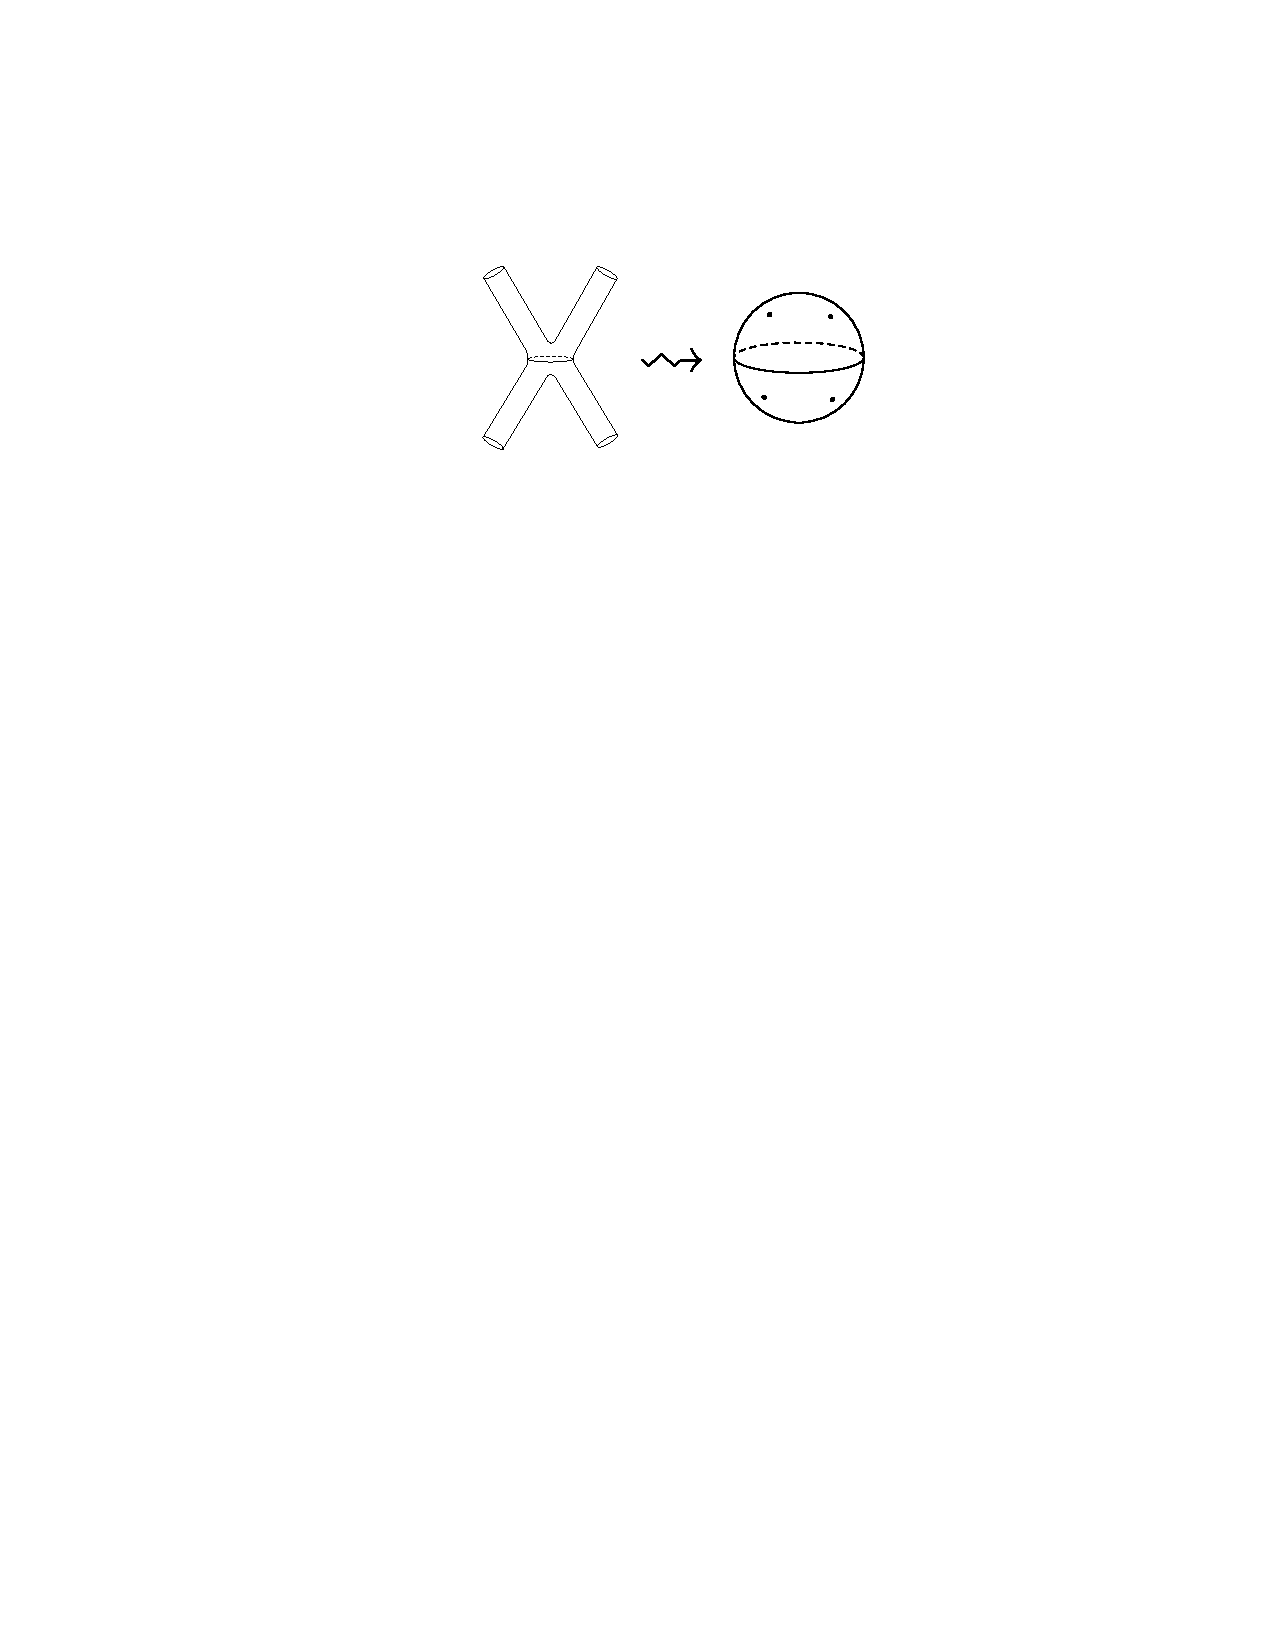
\includegraphics{figs/fig1.pdf}
	\caption{态算符对应与弦振幅}
	\label{fig:1}
\end{figure}
受前面配分函数的启发,由此可以写下弦振幅\footnote{也称作弦的S矩阵。}:
\begin{equation}
	\label{eq:2.39}
	\begin{aligned}
		S_{j_1...j_n}(k_1,\ldots,k_n)&=\llangle[\Big]\prod_{i=1}^n\int d^2\sigma_ig(\sigma_i)^{1/2}\mathscr{V}_{j_i}(k_i,\sigma_i)\rrangle[\Big]
		\\&=\sum_{\substack{\text{worldsheet}\\\text{topologies}}}\mathrm{e}^{-\lambda \chi}\int\frac{\mathcal{D}X\mathcal{D}g}{V_{\mathrm{diff}\times\mathrm{Weyl}}}\mathrm{e}^{-S_m}\prod_{i=1}^n\int d^2\sigma_ig(\sigma_i)^{1/2}\mathscr{V}_{j_i}(k_i,\sigma_i)
	\end{aligned}
\end{equation}
上式中我们使用$\llangle\bullet\rrangle$是为了提醒读者规范固定时可能的零模鬼场插入。而且上式我们并没有利用鬼场进行规范固定,这个问题我们留待到第\ref{chap:4}章解决。
\subsection{顶角算符}
利用前面正则量子化得到的激发态,只需要做如下替换便可以得到对应的顶角算符:
\begin{equation}
	\alpha_{-m}^\mu\to i\left(\frac{2}{\alpha^{\prime}}\right)^{1/2}\frac{1}{(m-1)!}\partial^mX^\mu(0),\quad
	|0;k\rangle\rightarrow e^{ik\cdot X(0,0)}
\end{equation}
由于算符乘积展开(OPE)在插入点相同时奇异,所以替换完成后还需要对算符取正规排序乘积(NOP)保证非奇异。这其实相当于一种重整化的选取,本论文均采用共形场论的NOP技术来重整化。

一般我们把上述构造的算符与世界面上积分$\int d\sigma^2$\footnote{注意开弦由于插入点在边界上,所以积分在边界上进行。}共同称作积分顶角算符,记作$U$,积分的存在使得顶角算符整体共形权为$0$,从而最终的振幅具有共形不变性。
\section{BRST量子化}
本节的核心目标是使用BRST量子化方法给出后续振幅计算中规范固定需要引入的无积分顶角算符。

考虑关于物质场$\phi_i$的某个一般性量子理论,$i$以及后续讨论涉及到的指标可以连续或离散,连续部分标记场的坐标依赖,离散部分则标记场的种类。假设所考虑体系的规范对称性生成元$\delta_\alpha$具有类似李代数的结构:
\begin{equation}
	\label{eq:2.41}
	[\delta_\alpha,\delta_\beta]=f_{\alpha\beta}^\gamma\delta_\gamma
\end{equation}
利用FP方法引入鬼场进行规范固定,规范选取为:
\begin{equation}
	F^A(\phi)=0
\end{equation}
则配分函数计算为:
\begin{equation}
	\int\frac{[d\phi_i]}{V_{\mathrm{gauge}}}\exp(-S_1)\to\int[d\phi_idB_Adb_Adc^\alpha]\exp(-S_m-S_g-S_f)
\end{equation}
这里新引入了鬼场$S_g$和规范固定项$S_f$:\footnote{前面\ref{eq:2.31}没有$S_f$是因为规范选取完全消除了$g$的规范冗余,不难看到$B_A$积分后的效果是引入$\delta(F^A(\phi))$,所以对$g$再次进行路径积分便完全移除了这一项。}
\begin{equation}
	S_g=b_Ac^\alpha\delta_\alpha F^A(\phi),\quad S_f=-iB_AF^A(\phi)
\end{equation}
以上无非是FP鬼场的一般做法,重点在于上述体系存在一个全局对称性:
\begin{equation}
	\begin{aligned}
		\delta_{\mathbf{B}}\phi_i 
		&= -i\epsilon c^\alpha\delta_\alpha\phi_i,  
		& \quad \delta_{\mathbf{B}}B_A 
		&= 0, \\
		\delta_{\mathbf{B}}b_{A} 
		&= \epsilon B_A,  
		& \quad \delta_{\mathbf{B}}c^{\alpha} 
		&= \frac{i}{2}\epsilon f^\alpha{}_{\beta\gamma} c^\beta c^\gamma.
	\end{aligned}
\end{equation}
对应的Noether荷记作$Q_B$,其中$\epsilon$是格拉斯曼变量。$c$的鬼数为$+1$,$b$和$\epsilon$鬼数为$-1$。所以$Q_B$具有$+1$的鬼数,而且具有幂零性:
\begin{equation}
	Q_{\mathrm{B}}^2=0
\end{equation}
考虑物质场和鬼场共同生成的希尔伯特空间,以鬼数为分次可以立即写下BRST上链复形$C^{\bullet}_{\mathrm{BRST}}$:
\begin{equation}
	\cdots\longrightarrow\mathscr{H}_{g-1}\xrightarrow{Q_{g-1}}\mathscr{H}_g\xrightarrow{Q_g}\mathscr{H}_{g+1}\longrightarrow\cdots
\end{equation}
BRST量子化则是要求物理态处于鬼数为0的上同调群中\footnote{对于无积分顶角算符则是要求在鬼数为1的上同调群中,而且额外要求是共形不变的,也就是限制在共形权为0的子复形中讨论上同调。},这其实是要求可观测量具有BRST不变性:\footnote{准确来说$\ket{\text{phys}}\in Z$,闭链要求给出BRST不变性,而模掉边缘链$B$(物理上也称$B$中的态为BRST恰当)意味着$B$中的态都是和物理态脱耦的,类似\ref{eq:2.26}}
\begin{equation}
	\label{eq:2.48}
	\mathscr{H}_{\mathrm{BRST}}\cong H^0(C^\bullet_{\mathrm{BRST}}):=Z(C^\bullet_{\mathrm{BRST}})/B(C^\bullet_{\mathrm{BRST}})
\end{equation}

接下来我们将上面一般性的方法应用到弦论中,BRST荷有如下形式:
\begin{equation}
	\label{eq:2.49}
	Q_B=\frac{1}{2\pi i}\oint(\operatorname{d}zj_B-\operatorname{d}\overline{z}\tilde{j}_B),\quad
	j_{\mathrm{B}}:=cT^m+:bc\partial c:+\frac{3}{2}\partial^2c
\end{equation}
$Q_B^2=0$要求$\{Q_B,Q_B\}=0$,这对应$j_B$OPE的一阶奇点:\footnote{这些复杂的OPE计算可以使用笔者编写的程序完成:\url{https://github.com/WHUZBF/MMA/tree/main/OPE}}
\begin{equation}
	j_B(z)j_B(w)\sim-\frac{c^m-18}{2(z-w)^3}c\partial c(w)-\frac{c^m-18}{4(z-w)^2}c\partial^2c(w)-\frac{c^m-26}{12(z-w)}c\partial^3c(w)
\end{equation}
由此可以看出自洽量子化要求$c^m=26$,也即靶空间维数为$26$。另外,物理态在壳要求:
\begin{equation}
	\label{eq:2.51}
	L_0|\psi\rangle=\{Q_B,b_0\}|\psi\rangle=0\Rightarrow b_0\ket{\psi}=0
\end{equation}
为了构造无质量态无积分顶角算符,首先使用$bc$鬼场物质场$\partial^n X$以及平面波$\mathrm{e}^{ip\cdot X}$构造出最一般的共形权为$0$的顶角算符:\footnote{注意我们这里忽视了鬼数为1这个条件,后面会在求BRST恰当项中引入。也可以先引入这个条件使得计算更加简便,但我们这里考虑最一般的构造帮助读者熟悉OPE计算。}
\begin{equation}
	V_{\text{general}}=:\left(\alpha\partial c+\beta c\partial^2c+\gamma c\partial c\partial^2c+\epsilon_\mu c\partial X^\mu+\zeta_\mu c\partial c\partial X^\mu+\lambda\right)e^{ip\cdot X}:
\end{equation}
上述对态的要求可以转化为对算符的要求:\footnote{这里我们利用了$Q$的定义含围道积分,对易子的计算可以转换为被积算符OPE的计算}
\begin{equation}
	Q_B\ket{\psi}=0\Leftrightarrow [Q_B,V] = 0 \Leftrightarrow Q_B V\sim 0
\end{equation}
首先作用在壳条件得到:
\begin{equation}
	\begin{aligned}
		&\begin{aligned}
		b_0V_{\text{general}}&=\oint\frac{\mathrm{d}z}{2\pi i}zb:\left(\alpha\partial c+\beta c\partial^2c+\gamma c\partial c\partial^2c+\epsilon_\mu c\partial X^\mu+\zeta_\mu c\partial c\partial X^\mu+\lambda\right)e^{ip\cdot X}:\\
		&=\oint\frac{\mathrm{d}z}{2\pi i}:\left(\frac{\alpha}{z}-\frac{\gamma c\partial^2c}{z}-\frac{\zeta_\mu(c\partial X^\mu)}{z}\right)e^{ip\cdot X}:=0\\
	\end{aligned}\\
	&\Rightarrow\alpha,\gamma,\zeta^\mu = 0
	\end{aligned}
\end{equation}
剩下的可能的顶角算符形式为:
\begin{equation}
	V_{\text{general}}\to V_1=:\left(\beta c\partial^2c+\epsilon_\mu c\partial X^\mu+\lambda\right)e^{ip\cdot X}:
\end{equation}
继续作用式\ref{eq:2.49},注意这里考虑开弦,只有左模:
\begin{equation}
	\begin{aligned}
		&Q_BV_1=\oint\frac{\mathrm{d}z}{2\pi i}\left[-\frac{i\alpha^{\prime}}{4z}\epsilon\cdotp:\partial^2ce^{ip\cdot X}c:+\frac{\lambda}{z}c\partial e^{ip\cdot X}\right]=0\\
	&\Rightarrow\lambda=0,\quad\epsilon\cdot p=0
	\end{aligned}
\end{equation}
注意到BRST算符并不改变共形权,所以BRST恰当部分应当也由$V_{\text{general}}$中的项生成,另外注意到鬼数为1的恰当项应当由鬼数为0的部分生成,而鬼数为零的算符只有平面波,所以我们立刻写下:
\begin{equation}
	Q_B\lambda :\mathrm{e}^{ip\cdot X}: = i\lambda:cp\cdot\partial Xe^{ip\cdot X}:
\end{equation}
这给出限制$\epsilon\cong\epsilon+p$,另外回到我们所关注的鬼数$1$上同调群,$c\partial^2 c$鬼数为$2$可以扔掉\footnote{凑巧它其实也是BRST恰当的},最终得到顶角算符:
\begin{equation}
	V_{\text{phys}}=:\epsilon_\mu c\partial X^\mu e^{ip\cdot X}:,\quad \epsilon\cdot p = 0,\epsilon^\mu\cong\epsilon^\mu+p^\mu
\end{equation}

上述计算推广到一般的态是显然的,开弦态只使用了左模场,闭弦态只需要额外使用右模场构造$V$即可。另外,虽然看似无积分顶角算符关联函数明显依赖于世界面坐标,后面会发现这一点被$V_{\mathrm{CKG}}$消除。

不难看出无积分顶角算符和积分顶角算符的联系为$V=cU$\footnote{如果是闭弦则是$V=c\tilde{c}U$},这是$bc$鬼场的性质,即便是RNS超弦这一点也成立,更重要的是这一联系也可以用BRST荷表述为:
\begin{equation}
	\label{eq:UV}
	[Q_B, U]\sim Q_B U= \partial V
\end{equation}
这在后面构造纯旋量超弦的积分顶角算符中非常重要。而且上式立刻说明了$\int\mathrm{d}z U(z)$ BRST闭,所以这也能看出$cU\leftrightarrow\int\mathrm{d}z U$。
\section{鬼场的真空}
现在我们来简要讨论上述结果的物理意义,这对后面构造RNS超弦顶角算符具有很大的意义。首先我们需要区分一下共形场论中的$SL(2,\mathbb{C})$不变真空$\ket{1}$。以及物理上关注的真空$\ket{0}$。对于共形权为$h$的主场,其$SL(2,\mathbb{C})$不变真空定义为:
\begin{equation}
	\phi_{n>-h}\ket{1}=0
\end{equation}
而物理上真空态要求能量最低,$H\sim L_0$而且注意到$[L_n,\phi_m]=[(h-1)n-m]\phi_m$,所以一切$\phi_{m>0}$都会降低能量(共形权),所以:
\begin{equation}
	\phi_{n>0}\ket{0}=0
\end{equation}
不难看出两者一般而言是不同的,这一点对于鬼场这种中心荷为负数的奇异系统尤为显著。由于$c$鬼场共形权为$-1$,所以我们能够构造能量低于$SL(2,\mathbb{C})$不变真空的真空态:
\begin{equation}
	\label{eq:2.62}
	\left|c\right\rangle=c_{1}\left|1\right\rangle,\quad\left|(\partial c)c\right\rangle=c_{0}c_{1}\left|1\right\rangle
\end{equation}
而\ref{eq:2.51}中$b_0$的要求相当于选取$\ket{c}$而不是$\ket{(\partial c) c}$作为微扰展开的鬼场真空。这样我们就能将$V$中出现的$c$自然解释为鬼场真空的贡献。而且$c$的出现是必然的,$bc$鬼场$U(1)$对称性给出下面的Noether流:
\begin{equation}
	\label{eq:2.63}
	j_{b,c}(z)=-:b(z)c(z):
\end{equation}
由此可以用下面的OPE定义算符$\mathcal{O}_q$的鬼数$q$:
\begin{equation}
	j_{b,c}(z)\mathcal{O}_q(w)\sim\frac{q\mathcal{O}_q(w)}{z-w}\Leftrightarrow j_0\ket{q} = q\ket{q}
\end{equation}
而$j_g$其实不是主场,其存在共形反常,可以由下面OPE看出:
\begin{equation}
	T_{b,c}(z)j_{b,c}(w)\sim\frac{-3}{(z-w)^3}+\frac{j_{b,c}(w)}{(z-w)^2}+\frac{\partial j_{b,c}(w)}{z-w}
\end{equation}
所以$bc$鬼系统具有背景鬼数$Q_{b,c}=-3$,这给出厄米共轭修正$j_n^\dagger=(-1)^{\delta_{n,0}}j_{-n}-Q_{b,c}\delta_{n,0}$。这要求只有当关联函数的鬼数(考虑真空背景后)为$0$时关联函数才不为$0$。所以关联函数中出现带$c$的无积分顶角算符是必然的。后面会看到对真空背景鬼数的补偿相当于路径积分中插入一些鬼场零模,Riemann-Roch定理指出鬼场零模插入有如下关系:
\begin{equation}
	\label{eq:2.66}
	N_c-N_b=3-3g
\end{equation}
对于$g=0$的球面情况,注意到$b$鬼数为$-1$,$c$鬼数为$+1$,这正好补偿了$Q_{b,c}=-3$。更高亏格的情况会在第\ref{chap:4}章详细说明。

而前面我们提到过积分顶角算符$U$和无积分顶角算符$V$在振幅计算中都非常重要,具体来说$\int d\sigma U$和$cV$对应同一个态的不同版本的顶角算符。为了补偿鬼场真空背景荷,在球面上就必须选取三个积分顶角算符替换为积分顶角算符,从而才能得到非零的振幅。后面第\ref{chap:4}章会从路径积分的角度直接看出这一点。
\section{*BV形式}
BRST量子化方法适用的前提是规范对称性满足\ref{eq:2.41}的结构,但如果这一结构不满足,比如结构常数不再是常数,而与场本身有关,而且不再是李代数闭的。BRST量子化就需要被扩充为更一般的Batalin–Vilkovisky量子化。更多细节可以在\cite{Weinberg:1996kr,Erbin:2021smf,Henneaux:1994lbw}中找到。

现在考虑下面更一般的规范对称性满足的代数:
\begin{equation}
	\label{eq:2.59}
	[\delta_a,\delta_b]=F_{ab}^c(\phi)\delta_c+\lambda_{ab}^i\frac{\delta S_m}{\delta \phi^i}
\end{equation}
后面一项意味着在壳情况下规范对称性还是闭的,这是物理上的要求,要求在壳时对称性构成一个群。BV形式的核心思想是把鬼场不单单看作是人为引入的消去规范的场,而是看作与物质场同等地位。因为对于更复杂的规范对称性的情况,可能$\delta_a$(第零级规范)之间不是独立的,也就是说\ref{eq:2.59}是一个可约代数\footnote{$p$-形式规范对称性就是个很好的例子,因为$d^2=0$,所以规范参数之间亦有规范不变性,而Yang-Mills理论是$1$-形式的理论,所以用BRST方法就能很好地处理。}。也就是说即便是规范对称性的参数之间仍有规范不变性(第一级规范),这意味着为了消去规范对称性引入鬼场,而为了消去规范对称性参数之间的对称性又要引入鬼场的鬼场,如此循环往复,直到消到第$\ell$级规范时\ref{eq:2.59}不可约。上述过程可以用图表\ref{tab:1}描述。
\begin{table}[htbp]
	\centering
	\begin{tabular}{ccc}
		\hline % 顶部粗线(可选)
		level $0$ & $\delta\phi^i=\epsilon_0^{a_0}R_{a_0}^i(\phi^i)$ & $c_0^{a_0}$ \\ 
		\hline % 中等粗细线
		level $1$ & $\delta c_0^{a_0}=\epsilon_1^{a_1}R_{a_1}^{a_0}(\phi^i,c^{a_0})$ & $c_1^{a_1}$ \\ 
		\hline
		$\cdots$ & $\cdots $ & $\cdots$\\
		\hline
		level $n+1$ & $\delta c_n^{a_n}=\epsilon_{n+1}^{a_{n+1}}R_{a_{n+1}}^{a_n}(\phi^i,c_0^{a_0},\ldots,c_n^{a_n})$ & $c_{n+1}^{a_{n+1}}$ \\ 
		\hline % 底部粗线(可选)
	\end{tabular}
	\caption{BV形式的鬼场}
	\label{tab:1}
\end{table}

现在把所有的鬼场和物质场看作同等地位:
\begin{equation}
	\psi^r=\{c_n^{a_n}\}_{n=-1,...,\ell},\quad c_{-1}:=\phi
\end{equation}
第$0$级物质场鬼数为$0$,且格拉斯曼偶宇称,每向上一级鬼数增加$1$,且格拉斯曼反宇称。同时引入对应的反场$\psi^*_r$\footnote{注意这里我们使用$\bullet^*$而不是$\tilde\bullet$,因为前面$\tilde b$虽然我们称为“反鬼场”,但其实只是鬼场的右模部分。}。和对应的“正”场之间格拉斯曼宇称相反,且鬼数相加为$-1$,反场由反括号诱导的对偶空间定义:
\begin{equation}
	(A,B)=\frac{\partial_RA}{\partial\psi^r}\frac{\partial_LB}{\partial\psi_r^*}-\frac{\partial_RA}{\partial\psi_r^*}\frac{\partial_LB}{\partial\psi^r},\quad \partial_R:=\overset{\rightarrow}{\partial},\partial_L:=\overset{\leftarrow}{\partial}
\end{equation}
量子化后的路径积分表示为:
\begin{equation}
	Z=\int\mathrm{d}\psi^r\mathrm{d}\psi_r^*\mathrm{e}^{-W[\psi^r,\psi_r^*]/\hbar}
\end{equation}
推广的BRST对称性由下式生成:
\begin{equation}
	\delta_\epsilon F=\epsilon\mathcal{Q}_B F=(W,F)-\hbar\Delta F,\quad \Delta:=\frac{\partial_R}{\partial\psi_r^*}\frac{\partial_L}{\partial\psi^r}
\end{equation}
为了自洽地量子化,必须要求$\delta_\epsilon W =0$,这相当于:
\begin{equation}
	(W,W)-2\hbar\Delta W=0
\end{equation}
上式常被称为量子主方程,此方程用于将$S_m$扩充为更一般的满足推广的BRST对称性的作用量$W$从而进行量子化。$\mathcal{Q}_B$依旧是幂零算符,计算其上同调便可得到可观测量,这一点与BRST形式是一致的。
	\chapter{Ramond-Neveu-Schwarz超弦}
\label{chap:3}
本章平行于上一章的结构,利用正则量子化给出具有世界面超对称的RNS超弦理论的激发粒子谱以及对应的顶角算符,特别是通过引入GSO投影消去了快子态、得到了费米自由度和玻色自由度相匹配的粒子谱。为了后续计算的方便,本章使用了更为现代的超对称共形场论(SCFT)的语言,更多细节详见\cite{Green:2012oqa,Green:2012pqa,Polchinski:1998rr}。
\section{世界面超场}
考虑世界面超对称,Polyakov作用量\ref{eq:2.2}中为$X$引入世界面自旋$\frac12$超伴场$\Psi$,为$\gamma$引入世界面自旋$\frac32$超伴场$\chi$,他们都是世界面上的二维旋量。在世界面Wick转动后,RNS超弦作用量为\footnote{$\rho$是二维gamma矩阵。}:
\begin{equation}
	\begin{aligned}
		S_{\mathrm{RNS}}[X,\Psi,g,\chi]=&\frac1{4\pi}\int\mathrm{d}^2\sigma\sqrt{-g}\Big[-\frac1{\alpha^{\prime}}g^{\alpha\beta}\partial_\alpha X^\mu\partial_\beta X_\mu+\overline{\Psi}^\mu\rho^\alpha\nabla_\alpha\Psi_\mu\\&+(\overline{\chi}_\alpha\rho^\beta\rho^\alpha\Psi^\mu)\Big(\frac1{\sqrt{2\alpha^{\prime}}}\partial_\beta X_\mu+\frac18\overline{\chi}_\beta\Psi_\mu\Big)\Big]
	\end{aligned}
\end{equation}
对于闭弦,上述作用量的超对称荷有左右模部分,所以实际上是$\mathcal{N}=2$超对称,而超弦只有左模有贡献,所以是$\mathcal{N}=1$超对称。后面将会看到他们低能极限下的谱分别是$\mathcal{N}=2$超引力以及$\mathcal{N}=1$超对称Yang-Mills理论。

现在$\mathrm{diff}\times\mathrm{Weyl}$不变性被提升为$\mathrm{Super\mbox{-}diff}\times\mathrm{Super\mbox{-}Weyl}$不变性,类似\ref{eq:2.30}取等温坐标到共形规范下消去$g$,这里我们可以取超共形规范消去$\chi$,并且将Majorana旋量\footnote{二维情况下总可以选取$\rho$的实表示从而要求$\Psi$为实的,这在二维情况下意味着是Majorana旋量}$\Psi$分解成左右手Weyl旋量$\psi/\bar\psi$。最终得到世界面上的超对称共形场论的物质项:
\begin{equation}
	S=\frac{1}{2\pi}\int\mathrm{d}^2z\left(\frac{2}{\alpha^{\prime}}\partial X^\mu\overline{\partial}X_\mu+\psi^\mu\overline{\partial}\psi_\mu+\overline{\psi}^\mu\partial\overline{\psi}_\mu\right)
\end{equation}
同时可以引入玻色鬼场$bc$以及费米鬼场$\beta\gamma$:
\begin{equation}
	S_{\mathrm{gh}}=\frac{1}{2\pi}\int\mathrm{d}^2z\left(b\overline{\partial}c+\overline{b}\partial\overline{c}+\beta\overline{\partial}\gamma+\overline{\beta}\partial\overline{\gamma}\right)
\end{equation}
共形变换以及相应的超共形变换的能动张量为:
\begin{equation}
	\label{eq:3.4}
	\begin{gathered}
		\frac{\delta S_m}{\delta g}\sim T^\mathrm{m}(z)=-\frac{1}{\alpha^{\prime}}:\partial X\cdot\partial X:-\frac{1}{2}:\psi\cdot\partial\psi:\\
		\frac{\delta S_m}{\delta\chi}\sim G^\mathrm{m}(z)=i\sqrt{\frac{2}{\alpha^{\prime}}}\psi^\mu\partial X_\mu
	\end{gathered}
\end{equation}
由于$g,\chi$都没有动力学,$T^m,G^m$应当为$0$类似\ref{eq:2.22}作为约束出现。另外$bc\beta\gamma$鬼场总共对中心荷贡献$-15$,而玻色场贡献$D$,费米场贡献$\frac{D}{2}$,所以共形反常消去必须要求:
\begin{equation}
	\boxed{D_{\mathrm{super}}=10}
\end{equation}

后面的讨论主要针对左模。类似开弦边界条件\ref{eq:2.9}的边界条件选取消去作用量泛函导数的边界项贡献,最终加倍技巧后体现为左右模相等\ref{eq:2.35}。而对RNS超弦,类似的条件会导致世界面超场左右模之间相差正负号,从而给出两种不同的超场模展开:
\begin{equation}
	\psi_{\mathrm{NS}}^\mu(z)=\sum_{r\in\mathbb{Z}+\frac{1}{2}}\psi_r^\mu z^{-r-\frac{1}{2}},\quad\psi_{\mathrm{R}}^\mu(z)=\sum_{n\in\mathbb{Z}}\psi_n^\mu z^{-n-\frac{1}{2}}
\end{equation}
世界面超场应当看作是在复平面的双覆盖黎曼面上定义。世界面超流$G$以及$\beta\gamma$鬼场同样可以分为NS和R两个部分,只是$z$的指数依赖要根据共形权重写。后面会看到$R$部分负责产生费米子,NS部分负责产生玻色子。对于闭弦,边界条件\ref{eq:2.8}变化为超场可以满足周期性或者反周期性。左右模部分可以分别处于NS,R部分,所以总共有四个部分。

最后来讨论一下费米物质场的真空。玻色场的真空由$\alpha^\mu_{n\geq 1}$湮灭的$\ket{0;p^\mu}$生成,其中$p^\mu\propto\alpha^\mu_0$用来标记真空动量$p^\mu$。类似的,费米物质场真空也由对应的湮灭算符产生:
\begin{equation}
	\psi_{r\geq\frac12}^\mu\left|0,p\right\rangle_{\mathrm{NS}}=0,\quad \psi_{n\geq1}^\mu\left|0,p\right\rangle_{\mathrm{R}}=0
\end{equation}
$\psi_0$类似$\alpha_0$既不是产生也不是湮灭算符,而是用于标记简并的真空态。不过$\psi_0$只存在于R部分真空,所以NS部分的真空依旧直接是$\ket{0}_{\mathrm{NS}}$,而且这也正是$\frac12$共形权的$\psi$场的$SL(2,\mathbb{C})$不变真空。注意到$\psi_0$之间满足:
\begin{equation}
	[\psi_0^\mu,\psi_0^\nu]=\eta^{\mu\nu}
	\xleftrightarrow{\Gamma\sim\sqrt{2}\psi_0} [\Gamma^\mu,\Gamma^\mu]=2\eta^{\mu\nu}
\end{equation}
也就是说R部分真空应当处于$SO(9,1)$的旋量表示也就是十维Clifford代数表示中,是具有$2^5=32$个分量的Dirac旋量$\left|A^{\prime}\right\rangle_{\mathrm{R}}=\left|A\right\rangle\oplus|\dot A\rangle$,现在考虑$G^m=0$的限制要求,类似\ref{eq:2.23},对R部分有:
\begin{equation}
	G^m_{n\geq0}\left|\mathrm{phys}\right\rangle_{\mathrm{R}}=\sum_{m\in\mathbb{Z}}\alpha_m\cdot\psi_{m-n}\left|\mathrm{phys}\right\rangle_{\mathrm{R}}=0
\end{equation}
这个时候由于\ref{eq:3.4}中$G^m$部分$\psi$与$\partial X$之间OPE正则,量子化时顺序无关紧要,所以不需要引入类似\ref{eq:2.23}的正规排序常数\footnote{这其实也是因为鬼场和物质场对R真空的总真空能贡献为0。}。考虑$n=0$时类似$L_0=0$的质量在壳条件,物质场超流要求的在壳条件可以改写为下面的Dirac-Ramond方程:
\begin{equation}
	\label{eq:3.10}
	\left(p\cdot\Gamma+\frac{2\sqrt{2}}{\ell}\sum_{n=1}^\infty(\alpha_{-n}\cdot \psi_n+\psi_{-n}\cdot\alpha_n)\right)\left|\mathrm{phys}\right\rangle_{\mathrm{R}}=0
\end{equation}
上述方程对真空态退化为$p\cdot\Gamma\ket{0}=0$即Dirac方程。这一方程将每个Weyl分量从$16$缩减到$8$。后面GSO投影会对这一自由度再次进行修正。

NS真空是$SL(2,\mathbb{C})$不变真空,而R真空实际上可以看作是NS真空的激发态,自旋场\footnote{其本质来源于$\psi$的玻色化\cite{Blumenhagen:2013fgp,Schlotterer:2012zz},不过后续计算我们并不会过多使用$S_A$。}将这两个真空联系起来:
\begin{equation}
	\left|A^{\prime}\right\rangle_{R}=\lim_{z\to 0}S_{{A^{\prime}}}(z)\left|0\right\rangle_{NS},\quad 
	{}_R\left\langle A^{\prime}\right|=\lim_{z\to\infty}{}_{NS}\left\langle0\right|S_{{A^{\prime}}}(z)z^{D/8}
\end{equation}
$z^{D/8}$的出现是BPZ共轭的要求\cite{itocft},$S_A$的共形权为$\frac{D}{16}=\frac58$,其来自于R部分物质场真空能贡献,相应的NS部分物质场真空能贡献为0:
\vspace{1.5em}% 这里需要调
\begin{equation}
	\label{eq:3.12}
	a^{\mathrm{m}}_R=
	\eqnmarkbox[blue]{node1}{\frac{1}{24}c^{\mathrm{m}}}+
	\left(\eqnmark[red]{node2}{-\frac{1}{24}}+\tikzmarknode{node3}{\frac{1}{24}}\right)D=\frac{1}{16}D
\end{equation}
\annotate[yshift=1em]{right}{node1}{能动张量非初级场,共形变换贡献}
\annotate[yshift=-0.5em]{below,left}{node2}{玻色场贡献}
\annotate[yshift=-1em]{below,label below}{node3}{费米场贡献}
%\vspace{1em}
\section{正则量子化}
本节首先使用光锥量子化处理RNS超弦,好处是规范完全固定,正则量子化能方便看出粒子谱及其的超对称性。后面再使用BRST量子化来构造协变的顶角算符,后面的讨论以开弦为例。

玻色场的光锥规范依旧和第\ref{chap:2}章的讨论相同,费米场NS部分的光锥规范有如下的简单形式:
\begin{equation}
	\psi^+ = 0
\end{equation}
R部分同上式一样,唯一不同是保留零模,用于生成简并R真空。而$\psi^-$部分同样也可以用横向振动激发描述。所以$\psi^\pm$不再拥有动力学,我们只需要关注横向振动激发。粒子谱由$\psi^i_\bullet,\alpha^i_\bullet$作用在R和NS真空上得到。

NS部分的质量谱可以从$L_0^m$最高权限制给出的在壳条件推出:
\begin{equation}
	\label{eq:3.14}
	\alpha^{\prime}m^2_{NS}=\sum_{n=1}^\infty\alpha_{-n}^i\alpha_n^i+\sum_{r=1/2}^\infty r\psi_{-r}^i\psi_r^i-\frac{1}{2}
\end{equation}
这里$-\frac12$来源于\ref{eq:3.12}类似的计算,注意还要加上鬼场的贡献,同理R部分有:
\begin{equation}
	\alpha^{\prime}m^2_{R}=\sum_{n=1}^\infty\alpha_{-n}^i\alpha_n^i+\sum_{n=1}^\infty n\psi_{-n}^i \psi_n^i
\end{equation}
不过从\ref{eq:3.14}能看出NS部分依旧存在快子态。同样,也可以先量子化再引入限制条件进行协变量子化,约束条件为:
\begin{equation}
	\text{NS: }\begin{cases}
		\left(L_{0}-a_{{\mathrm{NS}}}\right)|\text{phys}\rangle_{{\mathrm{NS}}}=0,\\
		L_{n>0}\left|\text{phys}\right\rangle_{\mathrm{NS}}=0,\\
		G_{r\geq\frac12}\left|\text{phys}\right\rangle_{\mathrm{NS}}=0
	\end{cases}
	\quad
	\text{R: }
	\begin{cases}
		\left(L_0-a_\mathrm{R}\right)|\text{phys}\rangle_\mathrm{R}=0,\\
		L_{n>0}\left|\text{phys}\right\rangle_{\mathrm{R}}=0,\\
		G_{n\geq0}\left|\text{phys}\right\rangle_{\mathrm{R}}=0
	\end{cases}
\end{equation}
类似$\S$\ref{sec:2.1.3}的论断得到正规排序常数为:
\begin{equation}
	a_{\mathrm{NS}} = \frac12,\quad a_{\mathrm{R}}=0
\end{equation}
类似$\S$\ref{sec:2.1.3}的推导可以导出态空间$\mathscr{H}_{\mathrm{OCQ}}$,前面\ref{eq:3.10}我们其实已经用了协变量子化的思想给出费米子波函数的限制,这里不再赘述。由于我们的目标是弦振幅的计算,所以对正则量子化的讨论这里是相当简略的,细节可参阅\cite{Green:2012pqa}。
\section{GSO投影}
RNS形式只保证了世界面上的超对称性,而我们更应当要求保留十维靶空间的超对称性。这一点需要在量子化的基础上剔除一些态。定义如下的G宇称算符:
\begin{equation}
\begin{aligned}
		G_{NS}&=(-1)^{F+1}=(-1)^{\sum_{r=1/2}^\infty \psi_{-r}^i\psi_r^i+1}\\
	G_R&=\Gamma_{11}(-1)^{\sum_{n=1}^\infty \psi_{-n}^i\psi_n^i}
\end{aligned}
\end{equation}
其中$\Gamma_{11}=\Gamma_{0}\Gamma_{1}\ldots\Gamma_{9}$。GSO投影要求NS部分的态满足$G_{NS}=+1$,显然快子态不满足这一要求,所以被剔除了,基态变为无质量矢量玻色子激发$\psi^i_{-1/2}\ket{0}_{NS}$。对于R部分,为了要求处于$G_R$本征态,则是要求剔除掉一般的手征。也就是说如果我们选取$\ket{\alpha;+}_R$\footnote{其实记号$\alpha$就已经表明了$\Gamma_{11}=+1$,这里后面加个$+$只是为了符号更加清晰。}作为基态,那么投影到$G_R=+1$,反之投影到$G_R=-1$。也就是说在GSO投影下,R部分基态从$8\oplus 8$破缺成了仅含一个手征$8$。对于开弦来说,取左右手征完全只是人为约定。

但是对于闭弦,左右模的R部分真空完全可以取相同或者相反手征,然后再把两部分GSO投影后的谱拼起来,这就得到了表\ref{tab:2}所示两种不同的自洽的闭弦构造。
\begin{table}[htbp]
	\centering
	\begin{tabular}{c|cc}
		\hline
		 &Type IIA &Type IIB\\
		 \hline
		$m^2=0$ 
		&\(\displaystyle
			\begin{gathered}
				|\dot\alpha;-\rangle_{\mathrm{R}}\otimes|\alpha;+\rangle_{\mathrm{R}}\\\tilde{\psi}_{-1/2}^i|0\rangle_{\mathrm{NS}}\otimes \psi_{-1/2}^j|0\rangle_{\mathrm{NS}}\\\tilde{\psi}_{-1/2}^i|0\rangle_{\mathrm{NS}}\otimes|\alpha;+\rangle_{\mathrm{R}}\\|\dot\alpha;-\rangle_{\mathrm{R}}\otimes \psi_{-1/2}^i|0\rangle_{\mathrm{NS}}
			\end{gathered}
		\)
		&\(\displaystyle
		\begin{gathered}
			|\alpha;+\rangle_{\mathrm{R}}\otimes|\alpha;+\rangle_{\mathrm{R}}\\\tilde{\psi}_{-1/2}^i|0\rangle_{\mathrm{NS}}\otimes \psi_{-1/2}^j|0\rangle_{\mathrm{NS}}\\\tilde{\psi}_{-1/2}^i|0\rangle_{\mathrm{NS}}\otimes|\alpha;+\rangle_{\mathrm{R}}\\|\alpha;+\rangle_{\mathrm{R}}\otimes \psi_{-1/2}^i|0\rangle_{\mathrm{NS}}
		\end{gathered}
		\)\\
		\hline
	\end{tabular}
	\caption{Type IIA/B超弦}
	\label{tab:2}
\end{table}

他们是可定向的闭弦理论,本身构造是不包含超弦的,为了引入开弦可以通过额外引入D膜。现在来观察无质量谱构成的超多重态:
\begin{equation}
	\text{type IIA: }(\mathbf{8_v}+\mathbf{8_c})\otimes(\mathbf{8_v}+\mathbf{8_s}),\quad \text{type IIB: }(\mathbf{8_v}+\mathbf{8_c})\otimes(\mathbf{8_v}+\mathbf{8_c})
\end{equation}
\begin{itemize}
	\item[$\bullet$]NS-NS部分:A/B型弦论都是$\mathbf{8_v}\otimes\mathbf{8_v}=\mathbf{1}+\mathbf{28}+\mathbf{35}=\phi\oplus B_{\mu\nu}\oplus G_{\mu\nu}$,分解为伸缩子,反对称$B$-场以及引力子
	\item[$\bullet$]NS-R和R-NS部分:注意到$\mathbf{8_v}\otimes\mathbf{8_s}=\mathbf{8_c}\oplus\mathbf{56_s}$以及$\mathbf{8_v}\otimes\mathbf{8_c}=\mathbf{8_s}\oplus\mathbf{56_c}$。所以A/B型弦论的两个部分都给出伸缩超伴子和引力超伴子。但是A型超弦NS-R和R-NS的手性不一样,B型则相同
	\item[$\bullet$]R-R部分:对于A型超弦$\mathbf{8_c}\otimes\mathbf{8_s}=\mathbf{8_v}\oplus\mathbf{56_t}$,分解为1-形式(矢量场)规范场和3-形式规范场;对于B型超弦$\mathbf{8_c}\otimes\mathbf{8_c}=\mathbf{1}+\mathbf{2}\mathbf{8}+\mathbf{3}\mathbf{5_+}$,分解为0-形式(标量场)、2-形式和4-形式规范场。这些场统称为R-R形式场,类似Yang-Mills场作为1-形式场$A^\mu$在世界线上的拉回与点粒子相互作用,高形式场可以与更高维带R-R荷的D膜相互作用,这是D膜作为BPS态在超弦中稳定存在的关键。
\end{itemize}
而且不难看出费米子自由度和玻色子自由度至少在$m^2=0$层面上是吻合的。实际上GSO投影后,玻色子(NS部分生成)和费米子(R部分生成)生成函数为:
\begin{equation}
	\begin{gathered}
		f_{\mathrm{NS}}(w)=\frac{1}{2\sqrt{w}}\left[\prod_{m=1}^{\infty}\left(\frac{1+w^{m-1/2}}{1-w^m}\right)^8-\prod_{m=1}^{\infty}\left(\frac{1-w^{m-1/2}}{1-w^m}\right)^8\right]=\frac{\vartheta_3^4(\tau)-\vartheta_4^4(\tau)}{2\eta^{12}(\tau)}\\
	f_{\mathrm{R}}(w)=8\prod_{m=1}^\infty\left(\frac{1+w^m}{1-w^m}\right)^8=\frac{\vartheta_2^4(\tau)}{2\eta^{12}(\tau)}
	\end{gathered}
\end{equation}
其中$\vartheta_k(\tau)|_{w:=\mathrm{e}^{2\pi\mathrm{i}\tau}}$是Jacobi-$\theta$函数,$\eta(\tau)|_{w:=\mathrm{e}^{2\pi\mathrm{i}\tau}}$是Dedekind-$\eta$函数,定义可在\cite{Blumenhagen:2013fgp}中找到。利用$\vartheta^4_3-\vartheta^4_4=\vartheta^4_2$\cite{wzx,Hirschhorn2017}可立刻说明上述两生成函数等价,从而说明了在自由度层面靶空间超对称的保留。GSO投影本质其实来源于超弦圈级配分函数模不变性的要求。\cite{Polchinski:1998rr,Green:2012pqa,Blumenhagen:2013fgp}

本论文主要考虑开弦盘面振幅的计算,构造中即包含开弦谱的理论为I型超弦。其可以看作是由IIB型超弦将世界面宇称提升为规范对称性,从而取世界面$\mathbb{Z}_2$轨形投影得到,轨形不动点带来$O9$平面自然使得靶空间存在$D9$膜,而且由于需要消去引力反常,所以需要开弦带有$SO(32)$或$E_8\times E_8$对称性\footnote{利用Green-Schwarz机制消去反常还允许$E_8\times U(1)^{248}$和$U(1)^{496}$,不过\cite{PhysRevLett.105.071601}指出这两个李群其实无法自洽消去反常。},只有前者对应I型超弦,所以要求有32个$D9$膜存在,后者可以在杂交弦中发挥作用。这样得到的超弦也可以称作IB型超弦,IIA型超弦由于左右模手征不同,不存在世界面宇称对称性,所以无法直接通过轨形投影得到对应得I型超弦理论,但是可以先通过T对偶将IIA型超弦转换为IIB型超弦,再同时取世界面和靶空间$\mathbb{Z}_2$轨形投影得到IA型超弦。由于宇称作为规范对称性存在,所以I型超弦是非定向超弦。

本论文并不详细讨论自洽弦理论的构造问题,仅仅考虑弦论振幅本身的计算问题。

\section{RNS超弦顶角算符}
协变顶角算符的构造我们遵循\cite{Friedan:1985ge,Knizhnik:1985ke}给出的方案。
\subsection{超鬼场真空}
由于BRST量子化中鬼场也会同样贡献产生算符,前面玻色弦中$bc$鬼场真空存在一些问题,$\beta\gamma$鬼场则更加麻烦。在共形场论的语言下,OPE是最重要的东西,其地位等同于正则对易关系\footnote{其实最开始OPE就是作为场论量子化的替代途径引入的,后来由于CFT处于重整化群不动点,OPE形式简单,所以作为CFT的标准语言。},而玻色场OPE一般是$\ln(z-w)$形式,费米场OPE一般是$(z-w)^{-1}$的形式。玻色化和费米化的想法就是将玻色场分解为费米场,费米场满足某个OPE,但最终得到的玻色场OPE不变。而对于树图,或者说球面,OPE决定关联函数的奇异部分,但球面上全纯函数只能是个常函数,这意味着玻色化和费米化后不会改变关联函数,这为求解问题带来了极大的方便!利用这一思想我们将$\beta\gamma$进行费米化,然后将一个费米自由度再进行玻色化:
\begin{equation}
	\label{eq:3.19}
	\beta(z)=:\mathrm{e}^{-\phi(z)}:\partial\xi(z),\quad\gamma(z)=:\mathrm{e}^{\phi(z)}:\eta(z)
\end{equation}
详细的OPE见附录\ref{appendix:A}。类似$bc$鬼场$c$共形权$-1$带来的问题,$\gamma$鬼场共形权$-\frac12$导致$\gamma_{1/2}$作用于$SL(2,\mathbb{C})$上降低共形权但不将其湮灭。$bc$鬼场由于费米性带来的泡利不相容原理最多也只能允许作用一个$c_1$,但是$\gamma$满足玻色统计,这意味着真空共形权可以无限降低。另外对于R部分,$\beta\gamma$零模也会带来无穷多简并的真空,如何理解这一点是本节的核心。

利用\ref{eq:3.19}我们可以先给出一个临时的办法,也就是构造出一个基态,NS部分被$\gamma_{1/2}$湮灭,R部分被$\gamma_1$湮灭:\footnote{这一选取常常称为正则绘景。}
\begin{equation}
	\label{eq:3.20}
	\text{NS: }\left|q=-1\right\rangle_{\beta,\gamma}=:e^{-\phi(0)}:\left|0\right\rangle,\quad \text{R: }\left|q=-1/2\right\rangle_{\beta,\gamma}=:e^{-\phi(0)/2}:\left|0\right\rangle
\end{equation}
$:e^{q\phi}:$便会类似$c$一样出现在RNS无积分顶角算符中。类似\ref{eq:2.63},可以定义如下超鬼数流:
\begin{equation}
	\label{eq:3.21}
	j_{\beta,\gamma}(z)=-:\beta(z)\gamma(z):
\end{equation}
$\beta$鬼数$-1$,$\gamma$鬼数$+1$,$\mathrm{e}^{q\phi}$鬼数为$q$。
$\mathrm{e}^{q\phi}$超鬼数为$q$,其实在经过\ref{eq:3.19}的变换后,$\xi,\eta,\phi$系统存在一个新的守恒荷,称为绘景数:
\begin{equation}
	N_p=\oint\frac{dz}{2\pi i}(\xi\eta-\partial\phi)
\end{equation}
$\beta\gamma$本身的绘景数为$0$,所以用$\beta,\gamma$作用于真空上生成态空间不会改变绘景数。$\xi$鬼数为$+1$,$\eta$为$-1$,$\mathrm{e}^{q\phi}$为$q$。\ref{eq:3.20}相当于选取了一个“海拔最高”的真空,那么其它的更低能量的真空如何理解?类似Dirac当年为了解释反粒子引入费米子海的概念,这里我们应当引入玻色子海,认为所有低能量的真空都被完全填充,而且由于$\beta\gamma$鬼场是自由CFT,所以也不会造成真空不稳定衰变到其它真空的问题。从群表示的观点看,绘景数$q$相当于给出了不同的$\beta\gamma$鬼场的表示,而$:\mathrm{e}^{q\phi}:$沟通了这些不同真空。不同的真空上产生出的希尔伯特空间应当认为描述的是同一个态空间,只是他们带有不同的绘景数。

就像是$bc$鬼场对真空的影响,导致积分顶角算符和无积分顶角算符之间可以相互转换用于描述同一个物理态从而抵消$Q_{b,c}$。同样的,我们应该预期$\beta\gamma$也会有零模的插入,实际上\ref{eq:3.21}也不是共形初级场:
\begin{equation}
	T_{\beta,\gamma}(z)j_{\beta,\gamma}(w)\sim\frac{+2}{(z-w)^3}+\frac{j_{\beta,\gamma}(w)}{(z-w)^2}+\frac{\partial j_{\beta,\gamma}(w)}{z-w}
\end{equation}
真空带有背景超鬼数$Q_{\beta\gamma}=+2$,对于更一般的黎曼面有类似\ref{eq:2.66}:
\begin{equation}
	Q_{\beta,\gamma} = N_{\gamma}-N_{\beta}=2-2g
\end{equation}
注意到绘景数来源于$:\mathrm{e}^{q\phi}:$,其鬼数和绘景数都是$q$,所以背景超鬼数的补偿也可以看作是要求关联函数绘景数为$-2$。也就是说一个物理态会对应到多个不同绘景数的顶角算符,只要绘景数之和为$-2$,计算出来的弦振幅就是一样的。树级振幅只需要直到$-1\leq q\leq+\frac{1}{2}$的顶角算符便可以始终构造非零的关联函数,更高圈振幅需要更大绘景数的顶角算符。
\subsection{BRST量子化}
BRST流形式为:
\begin{equation}
	j_B=c\left(T+\frac{T_{b,c}+T_{\beta,\gamma}}{2}\right)-\gamma\left(G^m+\frac{G^{\mathrm{gh}}}{2}\right)
\end{equation}
其中$G^{gh}\sim\frac{\delta S_{gh}}{\delta\chi}$是鬼场超流,具体形式见附录\ref{appendix:A}。BRST荷可以利用超鬼荷分为三个部分:\footnote{但是总的鬼数还是$1$。}
\begin{equation}
	\begin{aligned}
		Q_{\mathrm{BRST}}&=\oint\frac{\mathrm{d}z}{2\pi i}j_{\mathrm{B}}(z)=Q_0+Q_1+Q_2\\Q_{0}&=\oint\frac{\mathrm{d}z}{2\pi i}\left(c(T+T_{\beta,\gamma})+:bc\partial c:\right)\\Q_{1}&=-\oint\frac{\mathrm{d}z}{2\pi i}:\gamma G^m:=-\oint\frac{\mathrm{d}z}{2\pi i}:\mathrm{e}^\phi\eta G^m:\\Q_{2}&=-\frac{1}{4}\oint\frac{\mathrm{d}z}{2\pi i}:b\gamma^2:=-\frac{1}{4}\oint\frac{\mathrm{d}z}{2\pi i}:b\mathrm{e}^{2\phi}\eta\partial\eta:
	\end{aligned}
\end{equation}
分成三部分原因是超鬼数作为守恒荷,最终BRST闭的态应当对每个鬼数的BRST算符分别闭,后面的计算会简便一些。剩下的就是利用$S_\alpha,\psi,X,b,c,\beta,\gamma$构造BRST闭的顶角算符,而且在顶角算符层面,NS部分只能含有奇数个$\psi$,R部分只能含有偶数个$\psi$而且自旋矩阵只能带手征Weyl指标,这些可以从关联函数单值性的要求看出。而且算符应当有$c:\mathrm{e}^{q\phi}:\Phi$的形式,记相应的积分顶角算符为$U:=:\mathrm{e}^{q\phi}:\Phi$。后面的讨论都在积分顶角算符下讨论,$Q_1,Q_2$的计算与$c$无关,而$Q_0$闭的要求转化为要求结果为全导数。\footnote{因为$cU(z)\leftrightarrow\int \mathrm{d}z U(z)$}计算下面的OPE:
\begin{equation}
	Q_0:cU: \sim (h_U-1):\partial c c U:
\end{equation}
所以$Q_0$闭仅仅要求$U$的共形权为$1$这相当于要求整体顶角算符共形权为$0$,利用$\mathrm{e}^{q\phi}$共形权为$-\frac{q^2}{2}-q$可以写下$\Phi$的共形权。考虑下面的$q=-1,-\frac12$绘景的顶角算符以及$q=0,\frac12$绘景的顶角算符:
\begin{equation}
	U^{q=-1,-\frac12} = \begin{cases}
		\Phi_{h=1/2}^{\mathrm{NS}}(z)\mathrm{e}^{-\phi(z)}\\
		\Phi_{h=5/8}^{\mathrm{R}}(z)\mathrm{e}^{-\phi(z)/2}
	\end{cases},\quad 
	U^{q=0,+\frac12} = \begin{cases}
		\Phi_{h=1}^{\mathrm{NS}}(z)\mathrm{e}^{0\phi(z)}\\
		\Phi_{h=13/8}^{\mathrm{R}}(z)\mathrm{e}^{+\phi(z)/2}
	\end{cases}
\end{equation}
上面左右两边描述不同绘景下的同一个物理态。事实上,绘景之间的变换有下面的关系:
\begin{equation}
	\label{eq:PCO}
	U^{(q+1)}=\mathcal{P}U^{(q)}=2[Q_{\mathrm{BRST}},\xi U^{(q)}]=2\oint_{\mathcal{C}(w)}\frac{\mathrm{d}z}{2\pi i }j_B(z)\left(\xi(w)U^{(q)}(w)\right)
\end{equation}

注意到$Q_{\mathrm{BRST}}$绘景数为$0$,$\xi$绘景数为$+1$,所以从绘景数的意义上上式良定义。另外,似乎构造出来的新算符是BRST恰当的,但是注意到$\xi$共形权为$0$,所以插入$\xi(z)$从算符对应的角度看相当于在态层面上插入$\xi_0$。注意到\ref{eq:3.19}中的构造,$\xi$始终是以$\partial\xi$的形式出现,类似于自由玻色场中$X$总是以$\partial X$的形式出现。这时$X$的零模$\alpha_0$不作为激发模式的生成元,而是作为真空态的好量子数,显然$\ket{0;k}$不会被看作是一个BRST恰当的态。同理$\xi_0$也只是用来沟通不同绘景,所以\ref{eq:3.19}虽然具有BRST恰当的形式,但本质上并没有与物理态脱耦。上式联系不同绘景等同于$bc$鬼场中联系积分和无积分顶角算符的\ref{eq:UV}。

下面来考虑无质量顶角算符的具体构造,后面我们不再使用上标区分NS和R部分,他们分别对应绘景数为$\mathbb{Z}$和$\mathbb{Z}+1/2$。考虑如下$q=-1$的顶角算符的构造:\footnote{后面提到顶角算符,都是在NOP的意义下定义的,后面省略符号$:\bullet:$。}\footnote{似乎到了RNS超弦,顶角算符鬼数明显不为$0$,这种超鬼数的非零复杂性可以从BRST算符可以分解为$Q_{0,1,2}$一瞥。但是最终可观测的关联函数保证无鬼。}
\begin{equation}
	\label{eq:3.30}
	U^{(-1)}(z)=\epsilon_\mu\psi^\mu(z)\mathrm{e}^{-\phi(z)}\mathrm{e}^{ik\cdot X(z)}
\end{equation}
$Q_0$由于共形权为$0$自动满足,计算$Q_1$:
\begin{equation}
	Q_1(z)U^{(-1)}(0)\sim \epsilon\cdot k\sqrt{\frac{\alpha^\prime}{2}}\oint \frac{\mathrm{d}z}{2\pi i}\frac{\eta(0)}{z^2}:\mathrm{e}^{ik\cdot X(z)}:\Rightarrow \epsilon\cdot k = 0
\end{equation}
另外注意到:
\begin{equation}
	Q_{\mathrm{BRST}}:\mathrm{-2\phi}\partial \xi\mathrm{e}^{ik\cdot X}:\sim k_\mu:\psi^\mu\mathrm{e}^{-\phi}\mathrm{e}^{ik\cdot X}:
\end{equation}
所以$\epsilon\cong\epsilon+k$。同样可以验证$R$部分有顶角算符:
\begin{equation}
	\label{eq:3.33}
	U^{(-\frac{1}{2})}(z)=u^\alpha S_\alpha(z)e^{-\frac{1}{2}\phi(z)}e^{ik\cdot X(z)}
\end{equation}
利用$\ref{eq:PCO}$可以得到更高绘景的顶角算符:
\begin{equation}
	\label{eq:3.34}
	\begin{aligned}
		U^{(+\frac{1}{2})}
		=&[Q_1+Q_0+Q_2,2\xi U^{(-\frac{1}{2})}]\\
		=&\frac{1}{\sqrt{\alpha^{\prime}}}u^\alpha\left\{e^{\frac{1}{2}\phi}(i\partial X^\mu+\frac{\alpha^{\prime}}{8}(k\cdot\psi)\psi^\mu)(\Gamma_\mu)_\alpha^{\dot{\beta}}S_{\dot\beta}\right\}e^{ik\cdot X}\\
		&\eqnmarkbox[blue]{node}{-2\partial(\xi cU^{(+\frac{1}{2})})+\frac{1}{2}b\eta e^{\frac{3}{2}\phi}u^\alpha S_\alpha e^{ik\cdot X}}\\
		\cong& U^{(-\frac12)}
	\end{aligned}
\end{equation}
\annotate[yshift=0em]{below,label above}{node}{decoupled}

最后两项的解耦性(至少在树图的解耦性),第一个是因为全导数在世界面积分后无贡献,第二个是因为树图不含$b$零模的插入。BRST闭要求费米子波函数满足Weyl方程$\slashed{p}u=0$。对于NS部分:
\begin{equation}
	\label{eq:3.35}
	U^{(0)}=\sqrt{\frac{2}{\alpha^{\prime}}}\epsilon_\mu\left(i\partial X^\mu+\frac{\alpha^{\prime}}{2}(k\cdot\psi)\psi^\mu\right)e^{ik\cdot X}\cong U^{(-1)}
\end{equation}

式\ref{eq:3.30},\ref{eq:3.33},\ref{eq:3.34}以及\ref{eq:3.35}构成了树图计算所需的全部顶角算符。它们对应的无积分顶角算符可以作用$c$得到,上面推导只是左模部分,对于右模部分只需要把左右模乘起来就好了比如$U^{(-1,0)}=U^{(-1)}\otimes \tilde U^{(0)}\cong U^{(0,0)}$,对应的无积分顶角算符可以作用$c\tilde{c}$得到。而IIA型和IIB型的区别体现在左右模顶角算符费米子波函数$u_A$带的Weyl指标是相同手征还是反手征。有质量态的顶角算符构造可以在\cite{Schlotterer:2012zz}中找到。

另外说一句,上面都是在升高$q$,反过来也可以问能不能找到$q<-1$,在作用绘景变换算符后得到$q\leq -1$。计算表明这样的顶角算符是解耦的,与任何物理态之间的关联函数都是0。正如前面所说$\ket{q=-1,-\frac12}$是“最高海拔”的真空。

现在来讨论绘景变换算符\ref{eq:PCO}形式的原因。通过计算不难发现$q=-1,0$绘景下的$\Phi^{\text{NS}}$之间有如下OPE:
\begin{equation}
	G^m(z)\Phi_h^{\text{NS}}(w)\sim\frac{\frac12\Phi_{h+\frac12}^{\text{NS}}}{z-w}
\end{equation}
从这里可以看出$(\Phi^{\text{NS}}_h,\Phi^{\text{NS}}_{\text{NS}})$构成超共形初级场对,他们由世界面超对称联系起来。提取上式的一阶极点留数有:
\begin{equation}
	\Phi_{h+1/2}^{\mathrm{NS}}(w)\mathrm{e}^{0\phi(w)}=2\oint\frac{\mathrm{d}z}{2\pi i}G^m(z)\Phi_h^{\mathrm{NS}}(w)=2(G^m_{-1/2}\Phi_h^{\mathrm{NS}})(w)
\end{equation}
所以绘景变换算符$\mathcal{P}$的作用可以看作是作用$G^m_{-r}$,R部分同样有此性质。也就是说绘景变换无非是世界面上的超对称变换,而RNS超弦天然保留世界面超对称性,所以从这个角度上不难理解不同绘景下的顶角算符在关联函数的意义上等价,所以在计算散射振幅时描述同一个物理态。也可以直接代入\ref{eq:PCO}进行验证,即证明下式:
\begin{equation}
		\langle\ldots V_i^{(q_i+1)}(z_i)\ldots V_j^{(q_j)}(z_j)\ldots\rangle\overset{?}{\operatorname*{\operatorname*{=}}}\langle\ldots V_i^{(q_i)}(z_i)\ldots V_j^{(q_j+1)}(z_j)\ldots\rangle
\end{equation}
插入绘景变换算符:
\begin{equation}
\begin{aligned}
		\bigg\langle\ldots\oint_{z_i}\frac{\mathrm{d}w}{2\pi i}j_{\mathrm{B}}(w)&\xi(z_i)V_i^{(q_i)}(z_i)V_j^{(q_j)}(z_j)\ldots\bigg\rangle\\&\overset{?}{\operatorname*{=}}
		\bigg\langle\ldots V_i^{(q_i)}(z_i)\oint_{z_j}\frac{\mathrm{d}w}{2\pi i}j_{\mathrm{B}}(w)\xi(z_j)V_j^{(q_j)}(z_j)\ldots\bigg\rangle
\end{aligned}
\end{equation}
这里就相当于在\ref{eq:4.21}中消除$V_{\text{CKG}}$插入$c$零模的处理,只是这里插入的是$\xi_0$,类似关联函数与$c$的插入点无关,$\xi$的插入点也可以随便更换:
\begin{equation}
\begin{aligned}
		\text{LHS} &= \sum_{k}\left\langle\ldots\oint_{\{z_k\neq z_i\}}\frac{\mathrm{d}w}{2\pi i}j_{\mathrm{B}}(w)V_i^{(q_i)}(z_i)\xi(z_j)V_j^{(q_j)}(z_j)\ldots\right\rangle\\
		&=\sum_{k}\left\langle\ldots\oint_{z_j}\frac{\mathrm{d}w}{2\pi i}j_{\mathrm{B}}(w)V_i^{(q_i)}(z_i)\xi(z_j)V_j^{(q_j)}(z_j)\ldots\right\rangle=\text{RHS}\\
\end{aligned}
\end{equation}
这里第一个等号利用了柯西定理更换围道,第二个等号利用了BRST闭的特性,如图\ref{fig:2}。
\begin{figure}[htbp]
	\centering
	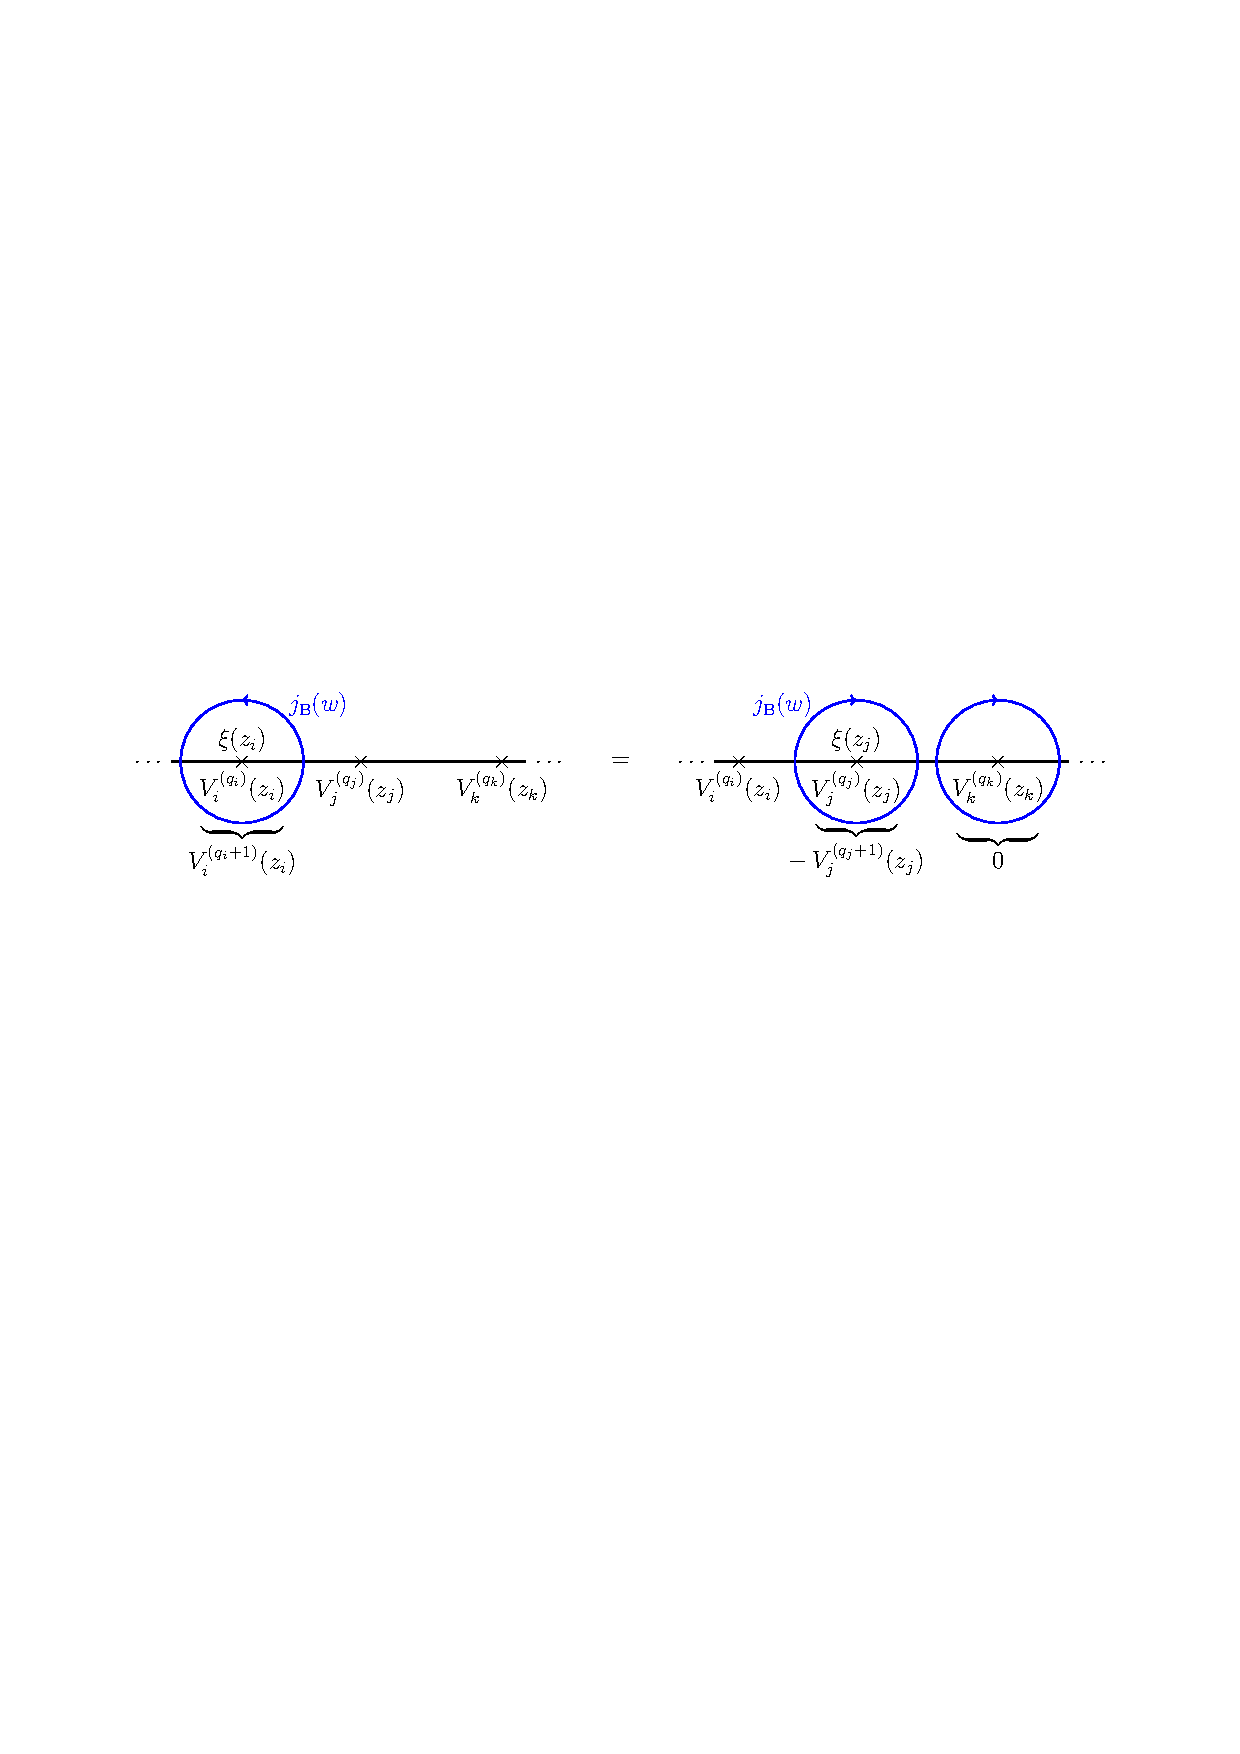
\includegraphics[width=\linewidth]{figs/fig2.pdf}
	\caption{围道替换}
	\label{fig:2}
\end{figure}

至此我们便完全说清了绘景变换对振幅无影响,在圈级振幅这对应一些绘景变换算符(Picture Changing Operator)的插入,同样可以进行类似讨论。\cite{Polchinski:1998rr}

	\chapter{弦微扰论}
\label{chap:4}
本节核心是将\ref{eq:2.39}的规范固定于黎曼曲面模空间相联系,并利用鬼场进行计算。弦微扰论目前前沿研究方向可见\cite{berkovits2022snowmasswhitepaperstring},超弦的规范固定比较复杂,详细可见\cite{Witten:2012bh}。本节还给出了一些玻色弦和超弦振幅的计算例子,以及Kawai-Lewellen-Tye关系\cite{Kawai:1985xq}和单值关系\cite{Bjerrum-Bohr:2009ulz}。

\section{模空间测度}
\ref{eq:2.39}的路径积分是对所有$\text{diff}\times\text{Weyl}$二维闭曲面等价类($\mathcal{D}g$)以及到靶空间的嵌入($\mathcal{D}X$)的求和。在数学上,$\text{diff}$的等价类由黎曼流形描述,多模去$\text{Weyl}$的等价类则由一维复流形,也就是黎曼曲面描述。我们首先从数学上对此进行叙述,这是代数几何中标准的内容\cite{forster2012lectures,schlichenmaier2010introduction,griffiths2014principles},我们选用更容易接受的物理些的讲法\cite{Giacchetto:2024aka,Staessens:2010vi}。
\subsection{黎曼曲面模空间}
黎曼曲面本身的定义是不含度规的,但是考虑在二维曲面$M$上加入不同的度规结构$[g]_{\text{diff}}$使之称为黎曼流形。下标$\text{diff}$提醒度量本身与坐标卡选取无关\footnote{在物理上微分同胚变换总是用不严谨的坐标变换替代,而数学上更偏向使用坐标无关的语言。}。可以证明任意一个度规结构$g$都给定了$M$上的复结构,而且此复结构仅仅依赖于度规的共形结构,也就是等价类$[g]_{\text{diff}\times\text{Weyl}}$,反过来,任意一个黎曼曲面都存在唯一一个与复结构相容的共形结构$[g]$。这样我们就把${\mathcal{D}[g]_{\text{diff}\times\text{Weyl}}}$的计算彻底与黎曼曲面上的复结构关联起来了。

类似微分同胚的定义,可以给出黎曼曲面之间全纯同构(共性等价)的概念,全纯同构对黎曼曲面进行了非常强的划分:

\begin{boxedtext}[单值化定理]
任何黎曼曲面$M$都共形等价于$\hat{M}/\pi_1(M)$,其中$\hat{M}$为$M$的泛覆叠空间,有下面几种情况:
\begin{equation*}
	\hat{M}=\left\{\begin{array}{c}\mathbb{C}\cup\{\infty\}\cong\mathbb{CP}^1\\\mathbb{C}\\\mathbb{H}\end{array}\right.
\end{equation*}
其中$\mathbb{H}$是上半复平面。
\end{boxedtext}

但是我们真正希望考虑的是复结构,复结构对黎曼曲面的刻画比全纯同构细的多。或者说不同的复结构之间可以是全纯同构的。而复结构的刻画就依赖于黎曼曲面的模空间,记为$\mathfrak{M}_g$,下标$g$表示亏格。而亏格为$g$的黎曼面上的所有度量结构记作$\mathcal{M}_g$。

上面的叙述似乎较为抽象,更加具体的方法是利用复结构与$[g]$的一一对应:
\begin{equation}
	\label{eq:4.1}
	\delta g_{ab}=\mathrm{diff}\oplus\mathrm{weyl}\oplus\mathrm{moduli}=-2(P_1\delta\sigma)_{ab}+(2\delta\omega-\nabla\cdot\delta\sigma)g_{ab}+\sum_{k=1}^{\dim\mathfrak{M}_g}\delta t^k\partial_{t^k}\hat{g}_{ab}
\end{equation}
这里利用了$n$阶对称无迹张量$v$到$n+1$阶对称无迹张量$u$的算符$P_n$:\footnote{这里$|b|$表示$b$不参与下标对称化。}
\begin{equation}
	(P_nv)_{a_1\cdots a_{n+1}}\equiv\nabla_{(a_1}v_{a_2\cdots a_{n+1})}-\frac{n}{n+1}g_{(a_1a_2}\nabla_{|b|}v_{a_3\cdots a_{n+1})}^b
\end{equation}
且此算符是唯一的,其共轭算符$P_n^T$定义为:
\begin{equation}
	(P_n^Tu)_{a_1\cdot\cdot\cdot a_n}\equiv-\nabla_bu^b{}_{a_1\cdot\cdot\cdot a_n}
\end{equation}
式\ref{eq:4.1}中$\mathrm{diff}\oplus\mathrm{weyl}$是规范冗余,是等价类$[g]$内部的映射,而$\mathrm{moduli}$则是黎曼面上不同的复结构,是等价类之间的变换,$t^k$用来标记不同复结构。计算$\mathcal{D}[g]$首先要选取一个规范固定$\hat{g}$,然后利用$\mathrm{diff}\oplus\mathrm{weyl}$规范变换积分掉整个等价类$[\hat{g}]$,与$V_{\mathrm{diff}\times\mathrm{weyl}}$抵消,然后在模空间上进行积分跑遍所有的等价类$[g]$。先取规范固定,然后积分掉规范自由度的过程,可以用图\ref{fig:3}表示。思想其实和Yang-Mills理论一样,但是弦论中选取一个规范固定无法用规范变换$\zeta$跑遍所有的$\mathcal{D}g$,所以还需要最后用模空间积分遍历。
\begin{figure}[htbp]
	\centering
	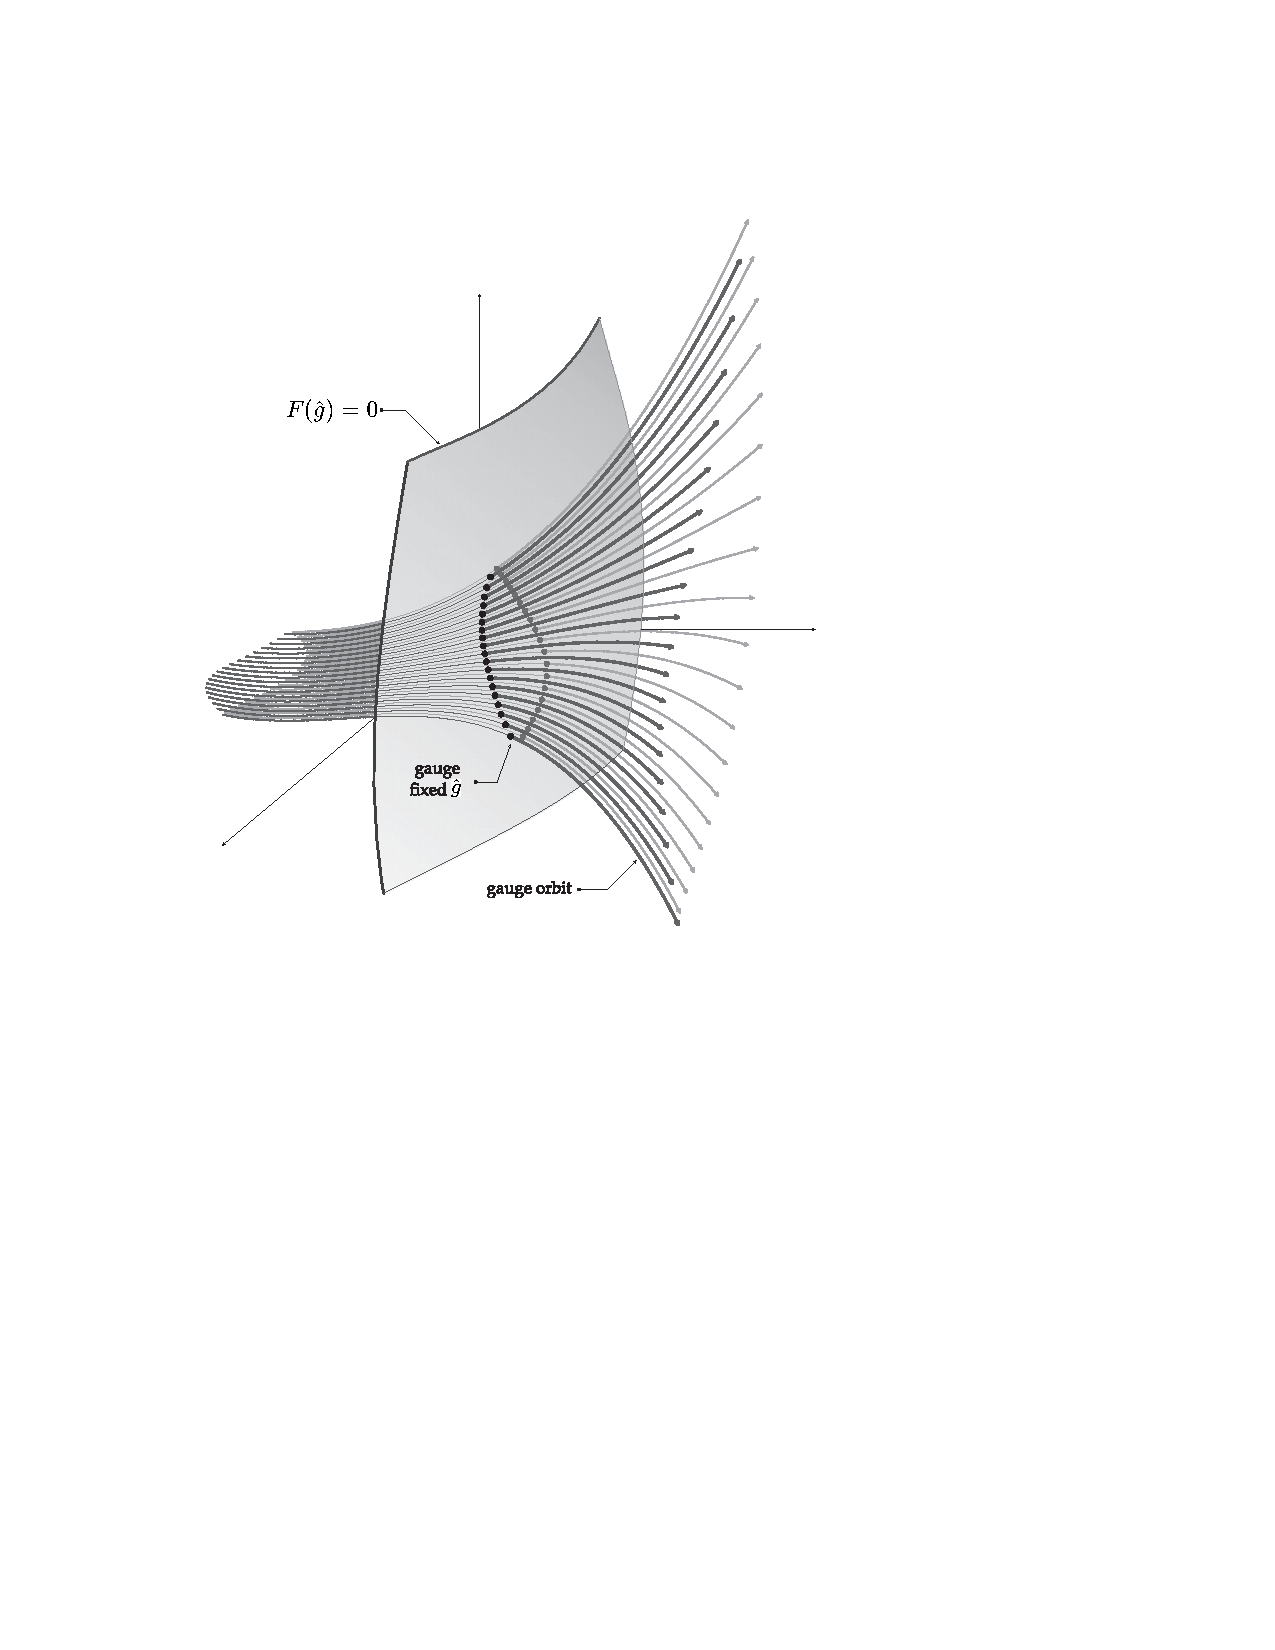
\includegraphics[width=0.5\linewidth]{figs/fig3.pdf}
	\caption{规范固定}
	\label{fig:3}
\end{figure}

虽然前面把$[g]$和复结构对应起来了,这告诉我们路径积分包含模空间的积分,但是为了对$\mathrm{diff}\oplus\mathrm{weyl}$积分,取规范固定$\hat{g}$后完全定下规范了吗?或者说我们建立了和规范变换$\zeta$和$[\hat g]$内元素的一一对应吗?这样$\int [\mathcal{D}\zeta]$才等于$V_{\mathrm{diff}\times\mathrm{weyl}}$从而完全消去规范冗余。但显然不是的,从前面光锥规范就能看出,单纯取等温坐标固定$g$没有完全定下规范,还又共形变换作为$\mathrm{diff}\oplus\mathrm{weyl}$的子群没有固定。同样的,规范变换$\zeta$跑遍了$[\hat g]$中的元素,但是$\mathrm{diff}\oplus\mathrm{weyl}$变换的子群CKG变换$\hat g$后仍得到$\hat g$,也就是说在规范固定点$\hat g$处仍有冗余的规范$V_{\mathrm{CKG}}$没有被消除。在数学上与之相关的群被称为黎曼曲面的自同胚群$\operatorname{Aut}(M)$。如果这个群是离散群,那么只需要除去$n_R=|\operatorname{Aut}(M)|$就可以消去规范,但是如果这个群是连续李群,这对应黎曼曲面$\pi_1(M)$是阿贝尔群的情况\footnote{对应的黎曼曲面称为例外黎曼面。},CKG的消去可以通过固定黎曼面上的某几个点来消去,也就是说规范选取变成了$(\hat g,\hat\sigma_{i\in\mathcal{F}})$,可以解释为固定了其中几个顶角算符的插入点\footnote{本文不考虑顶角算符个数不足以固定插入点的情况。},具体是固定哪几个顶角算符以及固定点的坐标$z_{i\in\mathcal{F}}$并不会影响最终的关联函数结果。自然联想到这种顶角算符的固定是通过积分顶角算符到无积分顶角算符之间的转换实现的,后面会看到的确如此。

上面规范固定的过程可以看作是下面的积分测度变换:
\begin{equation}
	\label{eq:4.4}
	\mathcal{D}gd^{2n}\sigma\to|J|\mathcal{D} \zeta d^{\mu}td^{2n-\kappa}\sigma
\end{equation}
其中$|J|$是变换的雅可比行列式。其中$\mu = \dim\mathfrak{M}_{g,n}$,$\kappa$则是CKG生成元个数。注意,在黎曼曲面上固定一个点需要一个“复”的CKG生成元,也就是一对实的CKG生成元来固定,例外是对于开弦顶角算符,由于其插入点在盘面边界圆周$\operatorname{Re}z=0$,所以只需要一个实的CKG生成元就能固定。后面谈到维数均指复维数。下面来计算几个简单黎曼面的自同胚群。

\begin{boxedtext}[黎曼曲面自同胚群]
	黎曼曲面$M$的自同胚群可以利用其基本群在其泛覆叠空间$\hat M$中的正规化子计算:
	\begin{equation*}
		\operatorname{Aut}(M)\cong N(\pi_1(M))/\pi_1(M),\quad N(G):=\{h\in \operatorname{Aut}(\hat{M})|hGh^{-1}=G\}
	\end{equation*}
\end{boxedtext}
所以首先要对三种不同的泛覆叠空间的自同胚群进行计算,结果如下:
\begin{equation}
	\operatorname{Aut}(\mathbb{CP}^1)\cong PSL(2,\mathbb{C}),\quad
	\operatorname{Aut}(\mathbb{C})\cong \operatorname{Aff}(1,\mathbb{C}),\quad
	\operatorname{Aut}(\mathbb{H})\cong PSL(2,\mathbb{R})
\end{equation}
注意到比如$\mathbb{CP}^1$和$\mathbb{H}$的自同胚群都包含两个连通分支,其中单位元存在的连通分支$\operatorname{Aut}_0(M)$才生成CKG。闭弦树级振幅涉及到球面,对应$\operatorname{Aut}_0(S^2)=SL(2,\mathbb{C})$,其有三个复自由度,所以可以固定球面上三个点。一圈振幅对应环面$\operatorname{Aut}_0(T^2)=\mathcal{T}_\mathbb{C}$,即由复平面上的平移群生成,所以可以在环面上固定一个点。同时离散对称性$\sigma^a\to -\sigma^a$同样不会改变环面上的$\hat{g}$,这个$\mathbb{Z}_2$对称性给出$n_R=2$。开弦树级振幅对应盘面也即上半复平面,对应CKG为$\operatorname{Aut}_0(D_2)\cong SL(2,\mathbb{R})$,有三个实自由度,所以同样可以固定盘面边界上三个顶角算符插入点。

模去共形Killing群后,我们考虑的黎曼曲面$\mathcal{M}_g$变成了带标记点的黎曼曲面$\mathcal{M}_{g,n}$,现在来关注其模空间$\mathfrak{M}_{g,n}$。注意到$\delta_m g_{ab}$与$\mathrm{diff\times weyl}$正交:
\begin{equation}
	\begin{aligned}
		0&=\int d^2\sigma g^{1/2}\delta_mg_{ab}\left[-2(P_1\delta\sigma)^{ab}+(2\delta\omega-\nabla\cdot\delta\sigma)g^{ab}\right]\\
		&=\int d^2\sigma g^{1/2}\left[-2(P_1^T\delta^{\prime}g)_a\delta\sigma^a+\delta_mg_{ab}g^{ab}(2\delta\omega-\nabla\cdot\delta\sigma)\right]\\
		&\Rightarrow  g^{ab}\delta_m g_{ab} =0,\quad (P^T_1\delta_m g)_a=0
	\end{aligned}
\end{equation}
第一个无迹条件自动满足,迹包含在Weyl变换项中,第二个条件说明模空间对应$\ker P^T_1$。另外CKG生成元满足的共形Killing方程可以写为:
\begin{equation}
	(P_1\delta\sigma)_{ab}=0
\end{equation}
所以CKG对应$\ker P_1$,模空间维数与CKG维数之间有如下公式:
\begin{boxedtext}[Riemann-Roch公式]
	\begin{equation}
		\label{eq:4.8}
		\dim\ker P_n-\dim\ker P_n^T=(n+\frac12)\chi=(2n+1)(1-g)
	\end{equation}
\end{boxedtext}
上式\ref{eq:4.8}只是Riemann-Roch定理的一个特例。注意到$\kappa$正好对应黎曼曲面上固定点的个数,所以上述结果可以推广到固定点任意多的黎曼曲面模空间:
\begin{boxedtext}[模空间维数]
	亏格为$g$且带$n$个标记点的黎曼曲面模空间是一个连通光滑的复轨形,维数为:
	\begin{equation}
		\label{eq:4.9}
		\dim\mathfrak{M}_{g,n} = 3 g - 3 + n
	\end{equation}
	且我们考虑$2g-2+n>0$情况,这对应$\operatorname{Aut}(M_{g,n})$是有限群,也即固定点后完全模去了CKG。
\end{boxedtext}
模空间是一个复轨形来源于其有如下的计算方式\footnote{考虑不带标记点的简单情况。}:
\begin{boxedtext}[Teichm\"uller空间]
	$\mathrm{Diff}^+$表示保定向的微分同胚变换,$\mathrm{Diff}_0$表示与单位映射同伦的微分同胚。则定义模群$\Gamma_g$\footnote{也常称为Mapping Class Group。}和Teichm\"uller空间$\mathfrak{T}_g$:
	\begin{equation*}
		\Gamma_\mathrm{g}:=\mathrm{Diff}^+(M)/\mathrm{Diff}_0(M),\quad \mathfrak{T}_\mathrm{g}\equiv\frac{\mathcal{M}_g}{\mathrm{Weyl}(M)\times\mathrm{Diff}_0(M)}
	\end{equation*}
	黎曼曲面模空间有如下轨形形式:
	\begin{equation}
		\label{eq:4.10}
		\mathfrak{M}_\mathrm{g}=\mathfrak{T}_\mathrm{g}/\Gamma_\mathrm{g}
	\end{equation}
\end{boxedtext}
利用\ref{eq:4.9}计算发现球面$g=0,n=3$情况模空间平凡,所以树图振幅不涉及模空间积分的计算。第一个非平凡的例子是环面$g=1,n=1$,模空间维数为$1$,环面上的复结构由下面的格生成:
\begin{equation}
	\Gamma:=\mathbb{Z}\alpha_1+\mathbb{Z}\alpha_2=\{n\alpha_1+m\alpha_2:n,m\in\mathbb{Z}\}
\end{equation}
$T^2 \cong  \mathbb{C}/\Gamma$,$\alpha_{1,2}\in\mathbb{C}$。不同复结构由$SL(2,\mathbb{Z})$意义下不同构的格生成。两个复自由度$\alpha_1,\alpha_2$约化为一个。在\ref{eq:4.10}的观点下,环面的模空间为:
\begin{equation}
	\mathfrak{M}_{1,1}=\mathbb{H}/PSL(2,\mathbb{Z})
\end{equation}
所以模空间参数$\tau$可以通过模群限制在图\ref{fig:5}所示的阴影部分中,即模空间积分范围为:
\begin{equation}
	\mathscr{F}:=\left\{\tau\in\mathscr{H}:-\frac{1}{2}\leq\mathrm{Re}(\tau)\leq\frac{1}{2},|\tau|\geq1\right\}
\end{equation}
这种模空间边界的自然存在性,或者说因为模不变性,让弦论自然拥有一个截断,从而是紫外有限的理论。\cite{Witten:2015mec}
\begin{figure}[htbp]
	\centering
	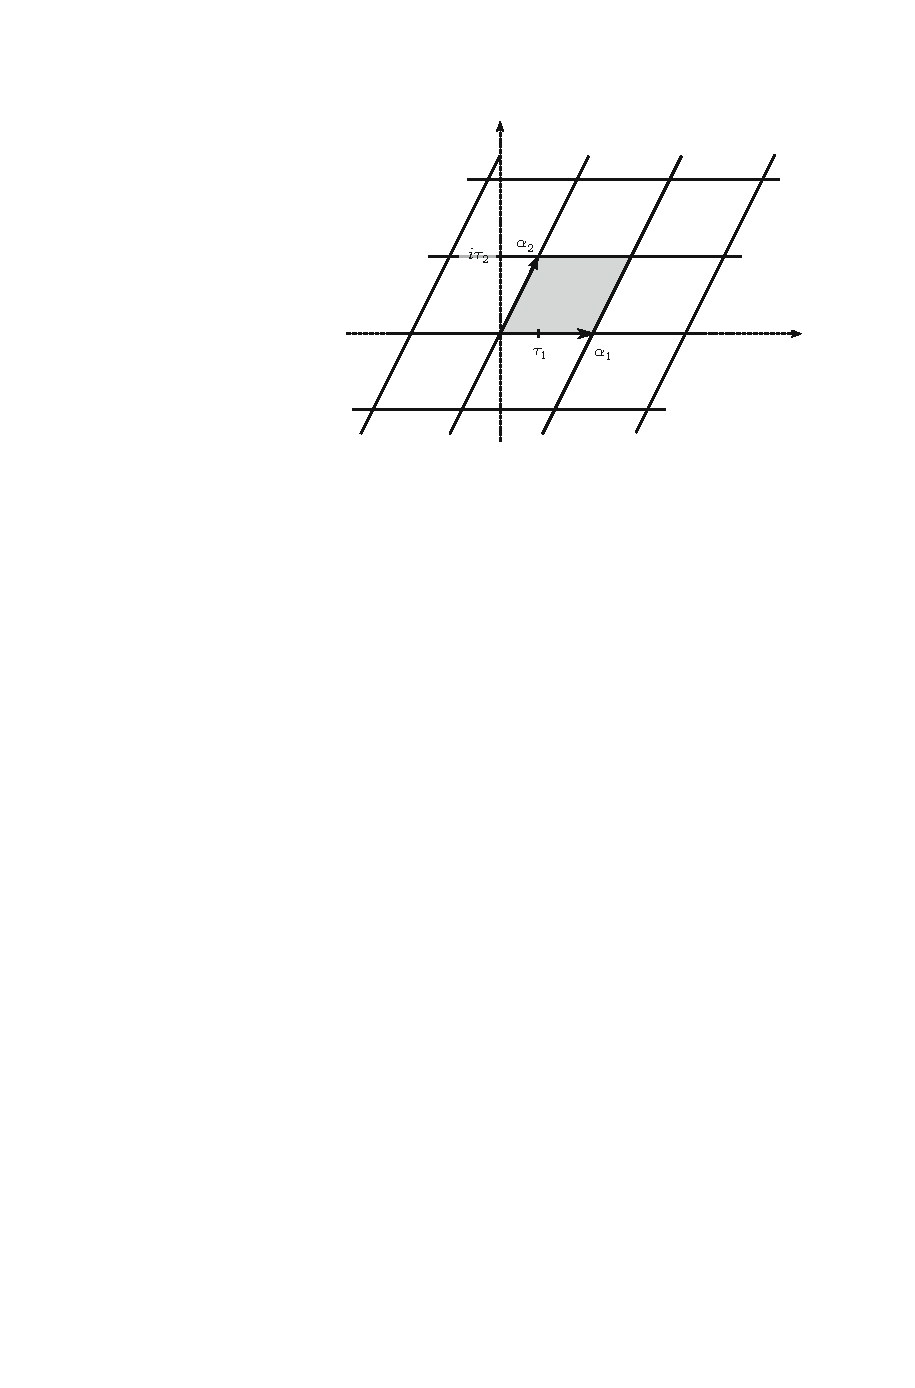
\includegraphics{figs/fig4.pdf}
	\caption{环面上不同的复结构,在$SL(2,\mathbb{Z})$同构的意义下,取$(\alpha_1,\alpha_2)=(1,\tau)$}
	\label{fig:4}
\end{figure}
\begin{figure}[htbp]
	\centering
	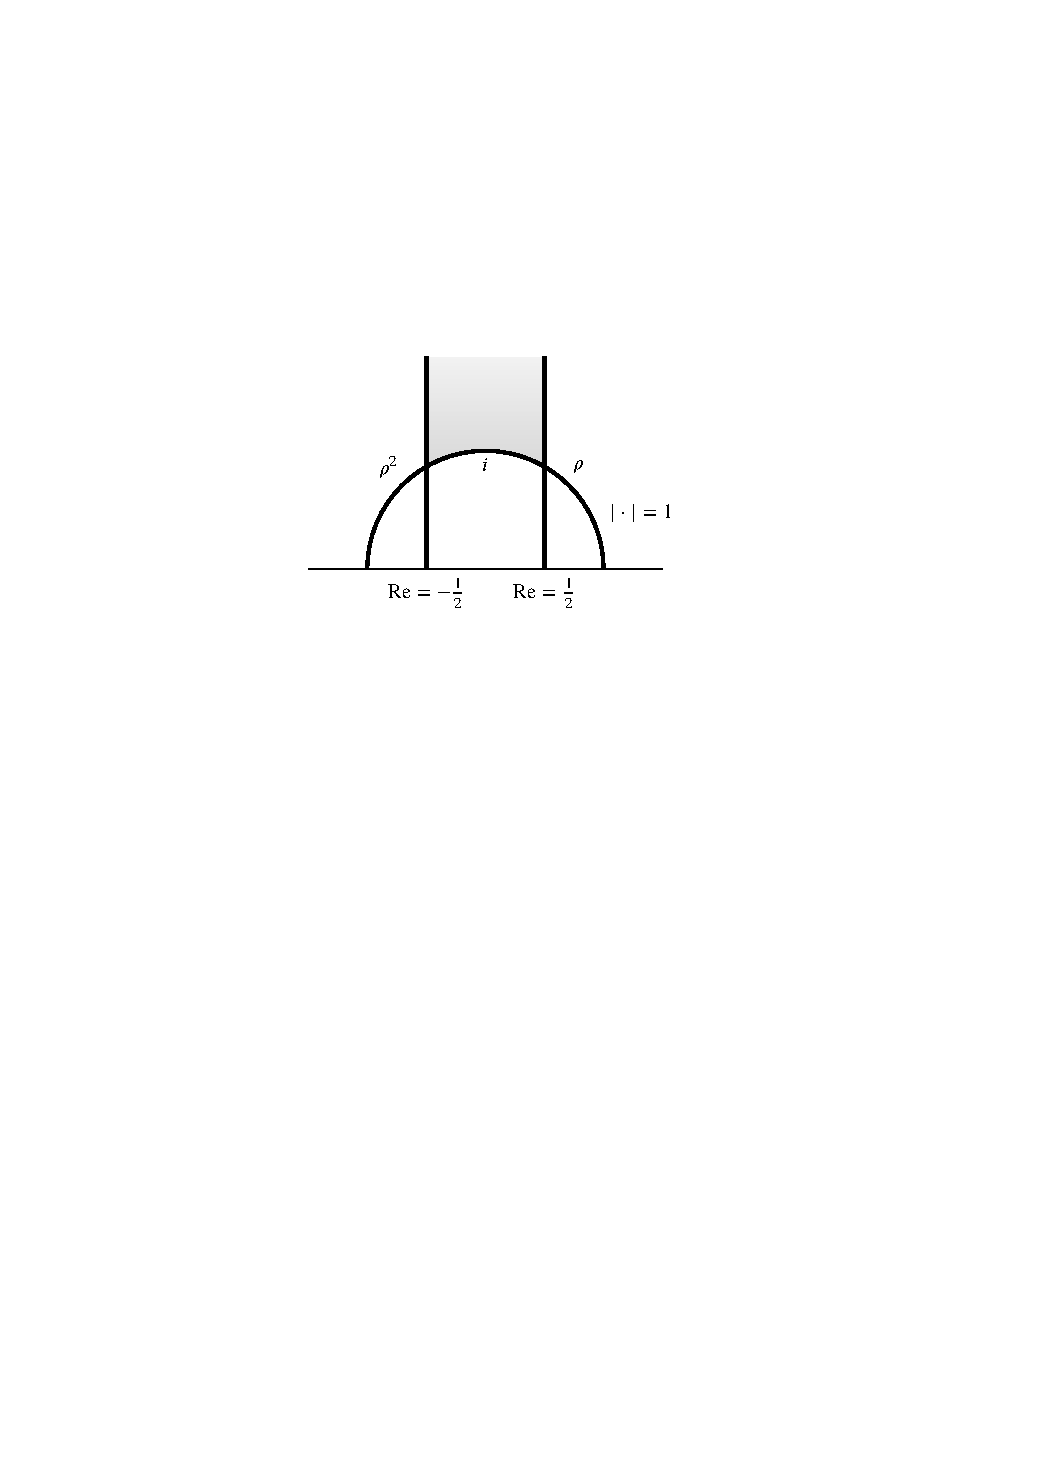
\includegraphics{figs/fig5.pdf}
	\caption{环面模空间的基本域,$\rho:=e^{2\pi i/6}$}
	\label{fig:5}
\end{figure}

在黎曼面上积分的想法近年来也从弦论渗透到了场论振幅计算中,Cachazo-He-Yuan形式给了场论振幅利用带标记点黎曼面上积分的统一形式\cite{Cachazo:2013iea,Cachazo:2013hca}:
\begin{equation}
	\mathcal{A}_{n}^\text{tree}=\int d\mu_{n}\mathcal{I}_{n}^L\mathcal{I}_{n}^R,\quad d\mu_{n}=\frac{d^{n}\sigma}{\mathrm{volSL}(2,\mathbb{C})}{\prod_{a}}^{\prime}\delta{\left(\sum_{b\neq a}\frac{s_{ab}}{\sigma_{ab}}\right)}
\end{equation}
不同场论的区别在于CHY被积函数$\mathcal{I}$,但是树级振幅都有上述的统一形式!
\subsection{FP量子化}
现在来计算\ref{eq:4.4}中的Jacobi行列式,这个积分测度变换对应插入:
\begin{equation}
	1=\Delta_{\mathrm{FP}}(g,\sigma)\int_\mathfrak{M}d^\mu t\int_\mathrm{diff\times Weyl}\mathcal{D}\zeta\delta(g-\hat{g}(t)^\zeta)\prod_{(a,i)\in \mathcal{F}}\delta(\sigma_i^a-\hat{\sigma}_i^{\zeta a})
\end{equation}
利用\ref{eq:4.1}以及标准的FP鬼场方法计算得到:
\begin{equation}
	\label{eq:4.16}
	\Delta_{\text{FP}}=\frac{1}{n_R}\int\mathcal{D}b_{ab}\mathcal{D}c^a\exp(-S_g)\prod_{k=1}^\mu\frac{1}{4\pi}(b,\partial_{t^k}\hat{g})\prod_{(a,i)\in \mathcal{F}}c^a(\hat{\sigma}_i),\quad S_g=\frac{1}{2\pi}\left(b,(\hat{P}_1c)\right)
\end{equation}
当$\hat g$取共形规范时$b_{ab}$和$c^a$退化为全纯和反全纯左右模,也即\ref{eq:2.32}形式。这里涉及到对称无迹张量之间的内积,定义为:
\begin{equation}
	\label{eq:4.17}
	(t,t^\prime)_{\hat g}:=\int d\sigma^a {\hat g}^{\frac{1}{2}} (t\cdot t^\prime)
\end{equation}
这里$\cdot$表示对所有指标缩并。\ref{eq:2.39}规范固定后的形式为:
\begin{equation}
	\label{eq:4.18}
	\begin{aligned}
		S_{j_1...j_n}(k_1,\ldots,&k_n)=\sum_{\substack{\text{worldsheet}\\\text{topologies}}}\int_{\mathfrak{M}}\frac{d^\mu t}{n_R}\mathcal{D}X\mathcal{D}b\mathcal{D}c\exp(-S_\mathrm{m}-S_\mathrm{g}-\lambda\chi)\\&\times\prod_{(a,i)\notin \mathcal{F}}\int d\sigma_i^a\prod_{k=1}^\mu\frac{1}{4\pi}(b,\partial_{t^k}\hat{g})\prod_{(a,i)\in\mathcal{F}}c^a(\hat{\sigma}_i)\prod_{i=1}^n\hat{g}(\sigma_i)^{1/2}U_{j_i}(k_i,\sigma_i)
	\end{aligned}
\end{equation}
由此可见固定顶角算符插入点确实相当于将无积分顶角算符换为积分顶角算符。现在对$bc$进行模展开,将上式与$bc$鬼场零模的插入联系起来。
\begin{equation}
	\label{eq:4.19}
	\begin{gathered}
		c^a(\sigma)=\sum_Jc_J\mathsf{C}_J^a(\sigma),\quad b_{ab}(\sigma)=\sum_Kb_K\mathsf{B}_{Kab}(\sigma)\\
		P_1^TP_1\mathsf{C}_J^a=\mu_J^{2}\mathsf{C}_J^a,\quad P_1P_1^T\mathsf{B}_{Kab}=\nu_K^2\mathsf{B}_{Kab}
	\end{gathered}
\end{equation}
$\mathsf{C}_J$,$\mathsf{B}_{K}$在\ref{eq:4.17}内积的意义下正交归一。而且两者的非零模之间有一一对应:
\begin{equation}
	\mathsf{B}_{Jab}=\frac{1}{\nu_J}(P_1\mathsf{C}_J)_{ab},\quad\nu_J=\mu_J\neq0
\end{equation}
而且零模正好是$\ker P_1^T$和$\ker{P_1}$中的向量。FP行列式\ref{eq:4.16}路径积分可以直接用模展开得到:
\begin{equation}
	\label{eq:4.21}
	\begin{aligned}
		\Delta_{\text{FP}}=&\int\prod_{k=1}^\mu db_{0k}\prod_{j=1}^\kappa dc_{0j}\prod_Jdb_Jdc_J\exp\left(-\frac{\nu_Jb_Jc_J}{2\pi}\right)\prod_{m=1}^\mu\frac{1}{4\pi}(b,\partial_{t^{m}}\hat{g})\prod_{(a,i)\in\mathcal{F}}c^a(\sigma_i)\\
		=&\int\prod_{k=1}^\mu db_{0k}\prod_{m=1}^\mu\left[\sum_{k^{\prime}=1}^\mu\frac{b_{0k^{\prime}}}{4\pi}\left(\mathrm{B}_{0k^{\prime\prime}},\partial_{t^m}\hat{g}\right)\right]
		\int\prod_{j=1}^\kappa dc_{0j}\prod_{(a,i)\in\mathcal{F}}\left[\sum_{j^{\prime}=1}^\kappa c_{0j^{\prime}}\mathsf{C}_{0j^{\prime}}^a(\sigma_i)\right]
		\\
		&\times\int\prod_Jdb_Jdc_J\exp\left(-\frac{\nu_Jb_Jc_J}{2\pi}\right)\\
		=&\det\frac{(\mathsf{B}_{0k},\partial_{t^m}\hat{g})}{4\pi}{\det}\mathsf{C}_{0j}^a(\sigma_i){\det}^{\prime}\left(\frac{P_1^TP_1}{4\pi^2}\right)^{1/2}
	\end{aligned}
\end{equation}
第二个等号利用了格拉斯曼变量积分的性质,只有在被积函数为积分变量的最高形式时才不为零。最后一个等号中${\det}^\prime$表示不考虑零模贡献,否则显然$\det=0$。由上式不难看出规范固定的过程正是插入$bc$鬼场零模,而Riemann-Sroch定理$\mu-\kappa$给出的正是鬼数补偿,其正好补偿背景鬼数\ref{eq:2.66}。

虽然鬼场方法是极具物理思想的方法,但是其推导出来的结果右有非常清晰的物理解释。\ref{eq:4.21}中第三项可以看作是一个归一化系数不用过多考虑,第二项$c$鬼场零模正好对应CKG生成元,第一项在数学上相当于插入一些Beltrami微分,是复结构的体现。而且,单纯从形式上来说\ref{eq:4.18}有下面更简单的形式:

注意我们将所有的顶角算符插入点全部固定,而增加了Beltrami微分,这也是鬼数补偿的要求。相当于考虑亏格相同,但是固定点更多的模空间:
\begin{equation}
	\mathfrak{M}_{g,n+n_c+n_o},\quad \dim\mathfrak{M} = -\frac32 \chi + \frac12 n_o+n_c
\end{equation}
固定点的信息被转移到了模空间中去。但是从计算的角度上看依旧是\ref{eq:4.18}更方便,因为模空间积分计算比较复杂。

前面都是对玻色弦考虑的,超弦的情况要复杂得多。对于本篇论文,只要知道树图是平凡的,我们只需要关注物质场关联函数计算以及$c$鬼场的插入即可。RNS超弦唯一多要求绘景数求和为$2$。
\section{树级关联函数计算}
本节计算树级物质场和鬼场的关联函数,直接从路径积分出发计算,并说明此结果于OPE计算得到的结果相同。这里我们只对玻色部分物质场进行计算,本章最后计算超弦振幅时会直接使用OPE计算费米部分关联函数。

观察玻色弦顶角算符,需要计算如下物质场关联函数:
\begin{equation}
	\label{eq:4.23}
	\left\langle\prod_{i=1}^n:e^{ik_i\cdot X(z_i,\bar{z}_i)}:\prod_{j=1}^p\partial X^{\mu_j}(z_j^{\prime})\prod_{k=1}^q\bar{\partial}X^{\nu_k}(\bar{z}_k^{\prime\prime})\right\rangle
\end{equation}
注意到:
\begin{equation}
	\label{eq:4.24}
	i\rho_j\cdot\partial Xe^{ik_j\cdot X(z_j)}=\left.\exp\bigg(i[k_j\cdot X(z_j)+\rho_j\cdot\partial X(z_j)]\bigg)\right|_{\text{linear in }\rho_j}
\end{equation}
所以我们只需要计算下面的关联函数即可得到\ref{eq:4.23}:
\begin{equation}
	\label{eq:4.25}
	\left\langle\prod_i:\exp\bigg(i\left[k_{i\mu}X^\mu(z_i)+\rho_{i\mu}\partial X^\mu(z_i)\right]\bigg):\right\rangle
\end{equation}
不妨考虑下面更一般的配分函数计算,$J=0$时即为真空配分函数:
\begin{equation}
	\label{eq:4.26}
	Z\left[J\right]=\left\langle\exp\left(i\int d^2\sigma J(\sigma)\cdot X(\sigma)\right)\right\rangle
\end{equation}
利用类似\ref{eq:4.19}的模展开技巧计算$\mathcal{D}X$:
\begin{equation}
	\begin{gathered}
		X^\mu(\sigma)=\sum_Ix_I^\mu\mathsf{X}_I(\sigma),\quad\nabla^2\mathsf{X}_I=-\omega_I^2\mathsf{X}_I,\quad \mathsf{X}_0=\left(\int d^2\sigma g^{1/2}\right)^{-1/2}\\ \left(\mathsf{X}_I,\mathsf{X}_J\right)=\delta_{IJ},\quad
	\mathsf{J}_I^\mu:=\int d^2\sigma J^\mu(\sigma)\mathsf{X}_I(\sigma)
	\end{gathered}
\end{equation}
带入到\ref{eq:4.26}得到:
\begin{equation}
	\label{eq:4.28}
\begin{aligned}
		Z\left[J\right]=&\prod_{I,\mu}\int dx_I^\mu\exp\left(-\frac{\omega_I^2x_I^\mu x_{I\mu}}{4\pi\alpha^{\prime}}+ix_I^\mu J_{I\mu}\right)\\
	=&i(2\pi)^d\delta^d(\mathsf{J}_0)\prod_{I\neq0}\left(\frac{4\pi^2\alpha^{\prime}}{\omega_I^2}\right)^{d/2}\exp\left(-\frac{\pi\alpha^{\prime}\mathsf{J}_I\cdot \mathsf{J}_I}{\omega_I^2}\right)\\
	=&i(2\pi)^d\delta^d(\mathsf{J}_0)\left({\det}^{\prime}\frac{-\nabla^2}{4\pi^2\alpha^{\prime}}\right)^{-d/2}\exp\left(-\frac{1}{2}\int d^2\sigma d^2\sigma^{\prime}J(\sigma)\cdot J(\sigma^{\prime})G^{\prime}(\sigma,\sigma^{\prime})\right)
\end{aligned}
\end{equation}
其中$G'$表示略去零模贡献的$X^\mu$格林函数:\footnote{对$\mathsf{X}_0$比较形象的解释源于世界面紧致,来源于传播带来的背景荷。}
\begin{equation}
	\label{eq:4.29}
	\begin{gathered}
		G^{\prime}(\sigma_1,\sigma_2)=\sum_{I\neq0}\frac{2\pi\alpha^{\prime}}{\omega_I^2}\mathsf{X}_I(\sigma_1)\mathsf{X}_I(\sigma_2)\\
	-\frac{1}{2\pi\alpha^{\prime}}\nabla^2G^{\prime}(\sigma_1,\sigma_2)=\sum_{I\neq0}\mathsf{X}_I(\sigma_1)\mathsf{X}_I(\sigma_2)=g^{-1/2}\delta^2(\sigma_1-\sigma_2)-\mathsf{X}_0^2
	\end{gathered}
\end{equation}
\ref{eq:4.28}计算中,$x^0_I$应当Wick转动到欧氏空间给出收敛的高斯积分,另外物质场零模需要单独处理,给出$\delta$函数,后面会进一步解释。注意,上面的计算结果原则上可以应用到任意世界面拓扑,只是格林函数有所不同。上式中取:
\begin{equation}
	\label{eq:4.30}
	J(\sigma)=\sum_{i=1}^n\left(k_i-\rho^a_i\partial_a\right)\delta^2(\sigma-\sigma_i)
\end{equation}
便得到了\ref{eq:4.25},但是去掉NOP。加上NOP的过程其实就是重整化的过程,注意到$G'(\sigma,\sigma)\to\infty$,记其不发散的全纯部分为$G^\prime_r$。\ref{eq:4.28}积分中$\sigma=\sigma'$时存在发散,将其重整化为$G^\prime_r(\sigma,\sigma)$发散便消除了。从共形场论的观点来看$G'(\sigma_i,\sigma_j)$是在计算$V_i,V_j$之间的缩并,而$G'(\sigma_i,\sigma_i)$是在计算$V_i$内部的缩并,显然发散,但顶角算符本身是定义在NOP意义下。所以把$G'$替换为$G'_r$就是将OPE重整化为NOP,去掉奇异项就是在去掉NOP内部的缩并。\footnote{回忆在计算NOP的缩并时,等价于不考虑NOP内部缩并,从而去除发散。}下面以球面上的计算为例说明这样做的后果。

取共形规范,在球面上求解\ref{eq:4.29}得到:
\begin{equation}
\begin{gathered}
	\label{eq:4.31}
		G^{\prime}_{S^2}(\sigma_1,\sigma_2)=-\frac{\alpha^{\prime}}{2}\ln|z_{12}|^2+f(z_1,\bar{z}_1)+f(z_2,\bar{z}_2)\\
	f(z,\bar{z})=\frac{\alpha^{\prime}\mathsf{X}_0^2}{4}\int d^2z^{\prime}\ln|z-z^{\prime}|^2+\mathrm{const}
\end{gathered}
\end{equation}
显然$G'$被分为奇异部分和全纯部分$G'_r$,为了简单起见取$\ref{eq:4.30}$中$\rho = 0$:
\begin{equation}
	\label{eq:4.32}
\begin{aligned}
		&\left\langle:e^{ik_1\cdot X(\sigma_1)}::e^{ik_2\cdot X(\sigma_2)}:\ldots:e^{ik_n\cdot X(\sigma_n)}:\right\rangle_\mathrm{S_2}\\
	=&iC_{S_2}^X(2\pi)^d\delta^d(\sum_ik_i)\times\exp\left(-\frac12\sum_{\substack{i,j=1\\i\neq j}}^nk_i\cdot k_jG^{\prime}(\sigma_i,\sigma_j)-\frac{1}{2}\sum_{i=1}^nk_i^2G_r^{\prime}(\sigma_i,\sigma_i)\right)
\end{aligned}
\end{equation}
不难发现物质场零模积分给出的$\delta$函数正好就是动量守恒,其中归一化常数将$\delta(\mathsf{J}_0)$的Jacobi行列式吸收后定义为:
\begin{equation}
	C_{S_2}^X=\mathsf{X}_0^{-d}\left({\det}^{\prime}\frac{-\nabla^2}{4\pi^2\alpha^{\prime}}\right)_{S_2}^{-d/2}
\end{equation}
这个归一化系数一般和模空间参数有关,而树图不涉及模空间积分,所以此归一化系数连带动量守恒$i(2\pi)^d\delta^d(\sum_i k_i)$在后续计算中全部略去。再利用$\ref{eq:4.31}$不难发现$f(z,\bar z)$贡献的项都$\propto\sum_i k_i$。从这个例子可以看出,在重整化加上NOP之后,只有格林函数的奇异部分会对关联函数有贡献,且求和时抛去$\sigma=\sigma'$的奇异项。而格林函数的奇异部分又正好对应OPE,也就是说(至少对于树图)关联函数的非零模部分积分可以直接由OPE计算奇异部分给出,而非奇异部分给出动量守恒$\delta$函数。这与球面上亚纯函数只与奇异性有关相吻合。前面计算是左右模共同的结果,球面上左右模独立传播,取全纯部分给出\ref{eq:4.25}结果:
\begin{equation}
	\label{eq:4.34}
	\prod_{i<j}(z_i-z_j)^{\frac{\alpha^{\prime}}{2}k_i\cdot k_j}\exp\left\{\frac{\alpha^{\prime}}{2}\sum_{i<j}\frac{\rho_i\cdot\rho_j}{(z_i-z_j)^2}+\frac{\alpha^{\prime}}{2}\sum_{i\neq j}\frac{k_j\cdot\rho_i}{(z_i-z_j)}\right\}
\end{equation}
乘上厄米共轭便得到左右模共同贡献,即关联函数:
\begin{equation}
	\left\langle\prod_i:\exp\bigg(i\left[k_{i\mu}X^\mu(z_i,\bar z_i)+\rho_{i\mu}\partial X^\mu(z_i)+\bar\rho_{i\mu}\bar\partial X^\mu(\bar z_i)\right]\bigg):\right\rangle
\end{equation}
利用\ref{eq:4.24}的技巧便可以得到振幅计算中物质场关联函数。同样的思路,下面考虑盘面情况。现在需要在有$\operatorname{Im} z = 0$的边界范围内求解\ref{eq:4.29},可以利用电像法求解,$\mathsf{X}_0$零模只贡献给非奇异部分,对最终关联函数无影响,可以扔掉:\footnote{这里使用$\sim$是为了指出格林函数原本应当还包含非奇异部分。}
\begin{equation}
	G^{\prime}_{D^2}(\sigma_1,\sigma_2)\sim-\frac{\alpha^{\prime}}{2}\ln|z_1-z_2|^2-\frac{\alpha^{\prime}}{2}\ln|z_1-\overline{z}_2|^2\overset{\operatorname{Im} z = 0}{\sim} -2\alpha^\prime \ln|y_1-y_2|
\end{equation}
\begin{figure}[htbp]
	\centering
	\caption{电像法计算格林函数}
	\label{fig:6}
\end{figure}
类似\ref{eq:4.32}的计算并注意到顶角算符均在实轴上插入:
\begin{equation}
	\label{eq:4.37}
	\begin{aligned}
		&\left\langle\prod_{i=1}^n :\exp\bigg(i\left[k_i\cdot X(y_i)+\rho_{i\mu}\partial X^{\mu}(y_i)\right]\bigg):\right\rangle_{D_2}\\
	=&\prod_{i<j}(y_i-y_j)^{2{\alpha^{\prime}}k_i\cdot k_j}\exp\left\{2{\alpha^{\prime}}\sum_{i<j}\frac{\rho_i\cdot\rho_j}{(y_i-y_j)^2}+2\alpha^{\prime}\sum_{i\neq j}\frac{k_j\cdot\rho_i}{(y_i-y_j)}\right\}
	\end{aligned}
\end{equation}
和\ref{eq:4.34}差别仅是$\alpha^\prime\to4\alpha^\prime$,$z\to y$。\ref{eq:4.34}和\ref{eq:4.37}指数项前面的因子是单纯平面波插入的关联函数,称为Koba-Nielsen因子。正如前面强调的,这些关联函数也可以直接从OPE出发计算。

剩下的就是鬼场关联函数,其实\ref{eq:4.21}就是在算剩下的鬼场关联函数,虽然从OPE来看非零模部分(如果没有$b$插入)无贡献,但是零模部分贡献非平凡。球面上\ref{eq:4.21}第一项由于模空间平凡所以无贡献,第三项是个归一化系数,记作$C^g_{S^2}$,所以只有$c$鬼场零模有贡献:
\begin{equation}
\begin{aligned}
		&\left\langle c(z_1)c(z_2)c(z_3)\tilde{c}(\bar{z}_4)\tilde{c}(\bar{z}_5)\tilde{c}(\bar{z}_6)\right\rangle_{S_2}\\
	\sim&\det\begin{vmatrix}1&1&1\\z_1&z_2&z_3\\z_1^2&z_2^2&z_3^2\end{vmatrix}\det\begin{vmatrix}1&1&1\\\bar{z}_4&\bar{z}_5&\bar{z}_6\\\bar{z}_4^2&\bar{z}_5^2&\bar{z}_6^2\end{vmatrix}=z_{12}z_{13}z_{23}\bar{z}_{45}\bar{z}_{46}\bar{z}_{56}
\end{aligned}
\end{equation}
上式可推广到球面上任意多个$b,c$鬼场插入:
\begin{equation}
	\left\langle\prod_{i=1}^{p+3}c(z_i)\prod_{j=1}^pb(z_j^{\prime})\cdot\widetilde{(\bullet)}\right\rangle_{S_2}=C^g_{S^2}\prod_{\substack{i,i^{\prime}=1\\i<i^{\prime}}}^{p+3}z_{ii^{\prime}}\prod_{\substack{j,j^{\prime}=1\\j<j^{\prime}}}^pz_{jj^{\prime}}^{\prime}\prod_{i=1}^{p+3}\prod_{j=1}^p(z_i-z_j^{\prime})^{-1}
\end{equation}
不难看到分母对应OPE给出非零模积分贡献,分子则来源于$c$鬼场零模贡献。对于开弦,左右模非独立传播,取上式的全纯部分即可。至此,我们已得到计算树级玻色弦振幅所需的所有关联函数,而超弦树级振幅关联函数由于涉及到自旋场还要麻烦些。

最后再来看另外一种计算鬼场关联函数的方法,这种视角在后面考虑纯旋量超弦时很有用,这里单纯以左模为例。前面\ref{eq:2.62}对鬼场真空进行了修正,在计算真空关联函数时,都要对真空泡泡图归一化,比如$SL(2,\mathbb{C})$真空$\braket{1}=1$。但是对于鬼场关联函数,必须要对真空背景鬼数进行补偿,所以其实$\braket{1}=0$,而鬼场修正后的真空应当归一化为$\braket{0}=1$。但是\ref{eq:2.62}给出了两个真空,应当归一化哪一个?其实无所谓,因为他们两个是厄米共轭的,也就是说:
\begin{equation}
	(c_1|1\rangle)^\dagger=\ket{c}^\dagger = \bra{(\partial c c)}=\langle1|c_{-1}c_0
\end{equation}
这是前面提到的鬼数流反常带来的效应,只有这样,合起来补偿鬼数$+3$,关联函数才不为零。那么,鬼场真空归一化应当表示:
\begin{equation}
	-\left\langle (c\partial c\partial^2c)(0)\right\rangle = \bra{1}c_{-1}c_0c_1\ket{1}=1
\end{equation}
由此便可以计算:
\begin{equation}
\begin{aligned}
		\left\langle c(z_1)c(z_2)c(z_3)\right\rangle &= \left\langle \left(\sum_{n=0}^\infty \frac{\partial^nc(0)}{n!}z_1^n\right) \left(\sum_{n=0}^\infty \frac{\partial^nc(0)}{n!}z_2^n\right)\left(\sum_{n=0}^\infty \frac{\partial^nc(0)}{n!}z_3^n\right)\right\rangle\\
		&=\left(z_1^2 z_2 - z_1 z_2^2 - z_1^2 z_3 + z_2^2 z_3 + z_1 z_3^2 - z_2 z_3^2\right)\cdot \left(-\frac12\left\langle (c\partial c\partial^2c)(0)\right\rangle\right)\\
	&= z_{12}z_{13}z_{23}\cdot\left(-\frac12\left\langle (c\partial c\partial^2c)(0)\right\rangle\right)\sim z_{12}z_{13}z_{23}
\end{aligned}
\end{equation}
差一个归一化常数,只需要更改一下真空归一化即可,这是无关紧要的。
\section{玻色弦振幅}
下文中用$\mathcal{A}$表示开弦树级振幅,$A$表示其色序振幅,$\mathcal{M}$表示闭弦树级振幅。类似Yang-Mills理论,Chan-Paton因子给出开弦树级振幅的色分解:
\begin{equation}
	\mathcal{A}_n=\sum_{\rho\in S_{n-1}}\mathrm{Tr}(\lambda^{a_{\rho(1)}}\lambda^{a_{\rho(2)}}\ldots \lambda^{a_{\rho(n-1)}}\lambda^{a_{n}})\times A(\rho(1),\rho(2),\ldots,\rho(n-1),n)
\end{equation}
色排序振幅指对世界面坐标积分时的某个顺序的贡献,比如$A(1,2,\ldots,n)$就代表$z_1<z_2<\cdots<z_n$的积分贡献。后面我们取规范固定$\{z_1,z_{n-1},z_n\}=\{0,1,\infty\}$,但是这不足以在$SL(2,\mathbb{R})$变换后得到所有色序,因为$SL(2,\mathbb{R})$变换保色序。比如上面的规范固定就一定是$z_1<z_{n-1}<z_n$\footnote{注意由于积分在盘面上,而不是真正在实轴上积分,或者说积分是在一维实射影空间中进行,所有的$<$都要在模去轮换的意义下理解。}。但显然还有$z_{n-1}<z_1<z_n$这种顺序,在这种色序下,取规范固定$\{z_1,z_{n-1},z_n\}=\{1,0,\infty\}$。闭弦规范固定就不涉及到这种顺序性,直接取$\{z_1,z_{n-1},z_n\}=\{0,1,\infty\}$即可。
\subsection{Veneziano 振幅}
考虑四快子振幅,其包含六个色序,如图\ref{fig:7}:
\begin{figure}[htbp]
	\centering
	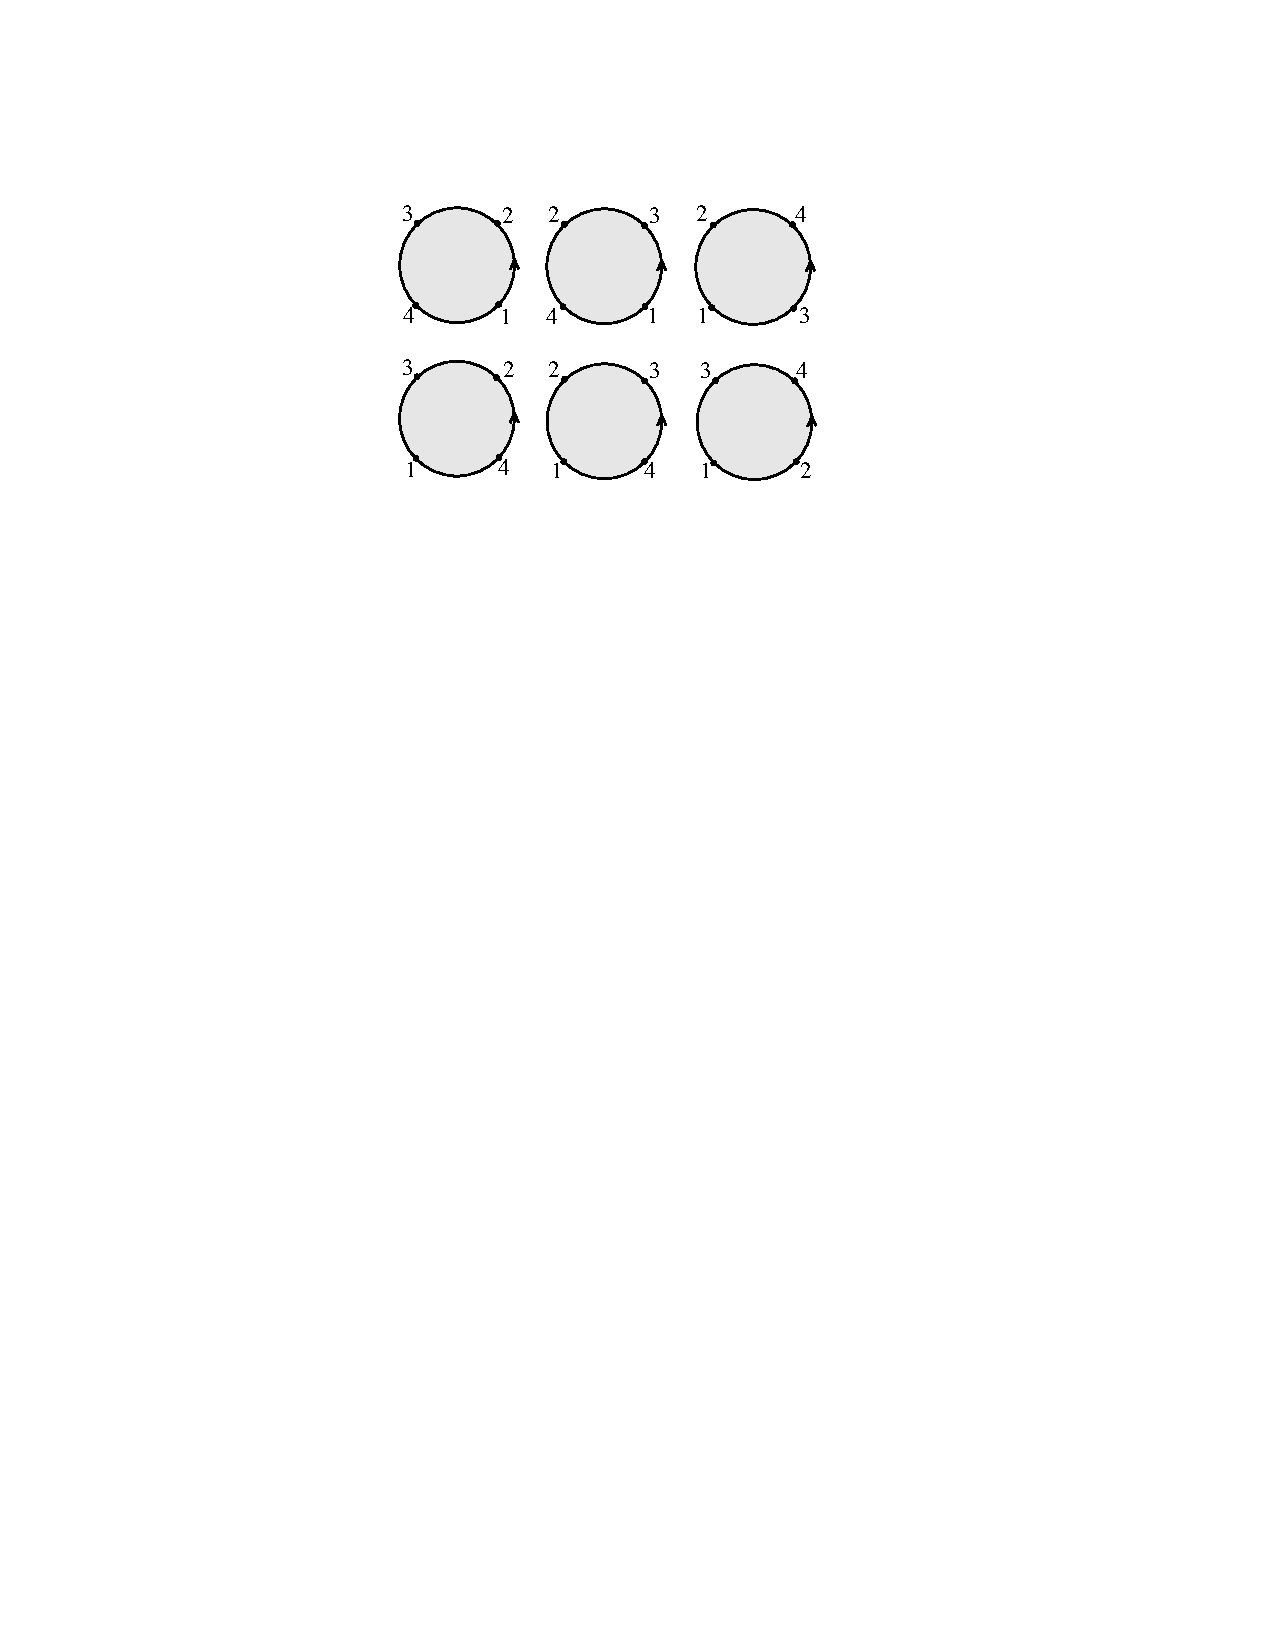
\includegraphics{figs/fig7.pdf}
	\caption{Veneziano振幅的六种色排序,上面三种取$\{z_1,z_{3},z_4\}=\{0,1,\infty\}$,下面三种取$\{z_1,z_3,z_4\}=\{1,0,\infty\}$。箭头方向表示正方向,越过$4$时由$+\infty\to - \infty$}
	\label{fig:7}
\end{figure}
\begin{equation}
\begin{aligned}
		&\mathcal{A}_4(\{T,a\}) \sim \left\langle\prod_{i=1,3,4}: c(y_i)e^{ik_i\cdot X(y_i)}:\int dy_2 e^{ik_2\cdot X(y_2)}\right\rangle\otimes \text{Chan-Paton}\\
	\sim&\int_{0}^1dy_2\mathcal{K}(\{0,1,\infty\};y_2)\operatorname{Tr}\left(\lambda^{a_1a_2a_3a_4}\right)+\int_{1}^\infty dy_2\mathcal{K}(\{0,1,\infty\};y_2)\operatorname{Tr}\left(\lambda^{a_1a_3a_2a_4}\right)\\
	&+\int_{-\infty}^0dy_2\mathcal{K}(\{0,1,\infty\};y_2)\operatorname{Tr}\left(\lambda^{a_2a_1a_3a_4}\right)+\int_{-\infty}^0 dy_2\mathcal{K}(\{1,0,\infty\};y_2)\operatorname{Tr}\left(\lambda^{a_2a_3a_1a_4}\right)\\
	&+\int_{0}^1dy_2\mathcal{K}(\{1,0,\infty\};y_2)\operatorname{Tr}\left(\lambda^{a_2a_3a_1a_4}\right)+\int_{1}^\infty dy_2\mathcal{K}(\{1,0,\infty\};y_2)\operatorname{Tr}\left(\lambda^{a_3a_1a_2a_4}\right)\\
\end{aligned}
\end{equation}
其中$\lambda^{abcd}:=\lambda^a\lambda^b\lambda^c\lambda^d$:
\begin{equation}
	\label{eq:4.42}
	\mathcal{K}(\{a_1,a_2,a_3\};y_2):=\lim_{\{y_1,y_3,y_4\}\to\{a_1,a_2,a_3\}}|y_{13}y_{14}y_{34}|\prod_{i<j}|y_{ij}|^{2\alpha^{\prime}k_i\cdot k_j}
\end{equation}
代入规范固定直接计算得到:
\begin{equation}
	\label{Veneziano}
\begin{aligned}
		\mathcal{A}_4(\{T,a\}) \sim&
	\operatorname{Tr}\left(\lambda^{a_1}\lambda^{a_2}\lambda^{a_4}\lambda^{a_3}+\lambda^{a_1}\lambda^{a_3}\lambda^{a_4}\lambda^{a_2}\right)B(-\alpha_0(s),-\alpha_0(t))\\
	&+\operatorname{Tr}\left(\lambda^{a_1}\lambda^{a_3}\lambda^{a_2}\lambda^{a_4}+\lambda^{a_1}\lambda^{a_4}\lambda^{a_2}\lambda^{a_3}\right)B(-\alpha_0(t),-\alpha_0(u))\\
	&+\operatorname{Tr}\left(\lambda^{a_1}\lambda^{a_2}\lambda^{a_3}\lambda^{a_4}+\lambda^{a_1}\lambda^{a_4}\lambda^{a_3}\lambda^{a_2}\right)B(-\alpha_0(s),-\alpha_0(u))
\end{aligned}
\end{equation}
其中$B$是Beta函数:
\begin{equation}
\begin{gathered}
		B(a,b)=\int_0^1dyy^{a-1}(1-y)^{b-1},\quad \alpha_o(x):= 1+\alpha' x\\
	s=-(k_1+k_2)^2,\quad t=-(k_1+k_3)^2,\quad u=-(k_1+k_4)^2
\end{gathered}
\end{equation}
\ref{Veneziano}就是Veneziano振幅\footnote{原始版本的不带色序,上式中所有迹贡献$1$。}。它是弦理论的第一个公式,原本是强相互作用的经验公式,后面才发现与快子振幅相关\cite{limiao}。早期这个公式有一个与场振幅截然不同的性质,对场振幅而言,四点树级振幅应当是s,t,u三个衰变道的求和。但弦振幅中不涉及到这种求和,换句话说,\ref{Veneziano}可以按照s,t或u的极点展开,极点位置正好是中间传播子在壳即满足\ref{eq:2.16}。但这三个道的展开是一样的,并不像场论中是不一样的展开,求和之后才是完整的振幅。所以弦振幅计算免去了场振幅中对所有费曼图求和的步骤,或者说弦振幅只需要计算一张图就可以了\footnote{当然这张图的计算麻烦得多。},一张图就包含了低能有效场论所有费曼图求和的信息。自然弦振幅也不涉及到场振幅中不同费曼图之间紫外发散的抵消。
\subsection{Virasoro-Shapiro振幅}
Virasoro-Shapiro振幅就是闭弦四快子振幅:
\begin{equation}
	\label{eq:4.45}
	\mathcal{M}_4(\{T\}) \sim \frac{2\pi\Gamma(-\frac{s}{4}-1)\Gamma(-\frac{u}{4}-1)\Gamma(-\frac{t}{4}-1)}{\Gamma(2+\frac{s}{4})\Gamma(2+\frac{u}{4})\Gamma(2+\frac{t}{4})}
\end{equation}
计算中需要用到如下公式:
\begin{equation}
	\int d^2_\mathbb{C}z|z|^{2a-2}|1-z|^{2b-2}=\frac{2\pi\Gamma(a)\Gamma(b)\Gamma(c)}{\Gamma(1-a)\Gamma(1-b)\Gamma(1-c)},\quad a+b+c=1
\end{equation}

现实世界不存在快子态,第一个非平凡的例子是三胶子振幅,其$\operatorname{Tr}(\lambda^{a_1}\lambda^{a_2}\lambda^{a_3})$的色序振幅有如下形式:
\begin{equation}
	\label{eq:4.47}
	A_3^{\text{gluon}}(1,2,3)\sim[(\varepsilon_1\cdot\varepsilon_2)(\varepsilon_3\cdot p_1)+\operatorname{cyc}(1,2,3)]+2\alpha^{\prime}(\varepsilon_1\cdot p_2)(\varepsilon_2\cdot p_3)(\varepsilon_3\cdot p_1)
\end{equation}
显然在$\alpha'\to 0$时就是Yang-Mills理论中(色序)三顶角费曼规则,$\alpha'$的存在暗示弦论的低能有效作用量中存在$\operatorname{Tr}(F^{n>2})$的高阶相互作用量。利用振幅的$\alpha'$展开计算弦论低能有效作用量也是目前弦振幅研究的重要前沿问题。而且由于弦振幅涉及到众多解析数论中的特殊函数,所以这一研究也和数学有很深刻的联系\cite{10.1007/978-3-030-37031-2_4,Stieberger:2016xhs}。

类似的,也可以有开弦闭弦混合振幅,开弦顶角算符在盘面边界圆周上插入,闭弦顶角算符在盘面内部插入,内部插入点积分范围为$|z|<1$。本文主要考虑纯开弦或纯闭弦振幅。文献\cite{dyj,Stieberger:2009hq}考虑了盘面开弦闭弦混合振幅及其与纯开弦振幅的关系。

\section{弦振幅之间的关系}
\subsection{单值关系}
开弦的色序振幅显然有轮换对称性以及:
\begin{equation}
	A_n^{\text{tree}}(1,2,\ldots,n)=(-1)^nA_n^{\text{tree}}(n,\ldots,2,1)
\end{equation}
本节的目的是给出非平凡的色序振幅之间的关系。而且单值关系完全只依赖于Koba-Nielsen因子的解析性质,和具体的顶角算符贡献无关。考虑四点情况,六种色序中有三种拥有相同的Koba-Nielsen因子\ref{eq:4.42},取$\{y_1,y_3,y_4\}={0,1,\infty}$,得到\footnote{也可以选$\{y_1,y_3,y_4\}={1,0,\infty}$规范固定下的另外三种色序得到额外的关系。}:
\begin{equation}
\begin{aligned}
	A_4(1,2,3,4)&=\int_0^1dy_2~|y_2|^{2\alpha^{\prime}k_1\cdot k_2}|1-y_2|^{2\alpha^{\prime}k_2\cdot k_3}\mathcal{V}_4(y_2)\\
	A_4(1,3,2,4)&=\int_1^\infty dy_2~|y_2|^{2\alpha^{\prime}k_1\cdot k_2}|1-y_2|^{2\alpha^{\prime}k_2\cdot k_3}\mathcal{V}_4(y_2)\\
	A_4\left(2,1,3,4\right)&=\int_{-\infty}^{0}dy_2~|y_2|^{2\alpha^{\prime}k_{1}\cdot k_{2}}|1-y_2|^{2\alpha^{\prime}k_{2}\cdot k_{3}}\mathcal{V}_4(y_2)
\end{aligned}
\end{equation}
这里$\mathcal{V}$表示顶角算符插入的贡献\footnote{这里利用了一个技巧,对于快子,前面的因子是正确的,但对于一般的顶角算符,由于固定点的位置完全是任意的,所以应当会贡献$|y_4|^\#$与Koba-Nielsen因子中的$|y_4|$幂次相抵消。否则$|y_4|\to\infty$时奇异。}。由于$\mathcal{V}$极点都在实轴上,而且按照大圆弧引理无穷远处围道贡献为$0$,得到:
\begin{equation}
\begin{aligned}
		0&=\lim_{\epsilon\to0^+}\int_{-\infty+i\epsilon}^{+\infty+i\epsilon}dy_2|y_2|^{2\alpha^{\prime}k_1\cdot k_2}|1-y_2|^{2\alpha^{\prime}k_2\cdot k_3}\mathcal{V}_4(y_2)\\
	&=\left(e^{2\pi i \alpha' k_1\cdot k_2}\int_{-\infty}^0+\int_0^1+e^{-2\pi i \alpha' k_2\cdot k_3}\int_1^\infty\right)\mathrm{d}y_2|y_2|^{2\alpha^{\prime}k_1\cdot k_2}|1-y_2|^{2\alpha^{\prime}k_2\cdot k_3}\mathcal{V}_4(y_2)\\
	&= e^{2\pi i \alpha' k_1\cdot k_2}A_4(2,1,3,4)+A_4(1,2,3,4)+e^{-2\pi i \alpha' k_2\cdot k_3}A_4(1,3,5,4)
\end{aligned}
\end{equation}
这里利用了绝对值在复平面上是多值函数,$\mathrm{e}^{-i\pi}$是因为$|1-y_2|$中$y_2$前的负号,所以相对$y_2$而言$(1,+\infty)$的积分是从实轴下面绕的。更一般的单值关系为:
\begin{equation}
	\label{eq:4.51}
\begin{gathered}
		A_n(\beta,1,\alpha,n)=(-1)^{|\beta|}\operatorname{Re}\left[\prod_{1\leq i<j\leq |\beta|}e^{2i\pi\alpha^{\prime}(k_{\beta_i}\cdot k_{\beta_j})}\sum_{\sigma\in\alpha\shuffle \beta^T}\prod_{i=0}^{|\alpha|}\prod_{j=1}^{|\beta|}e_\sigma^{(\alpha_i,\beta_j)}A_n(1,\sigma,n)\right]\\
	0=\operatorname{Im}\left[\prod_{1\leq i<j\leq |\beta|}e^{2i\pi\alpha^{\prime}(k_{\beta_i}\cdot k_{\beta_j})}\sum_{\sigma\in\alpha\shuffle \beta^T}\prod_{i=0}^{|\alpha|}\prod_{j=1}^{|\beta|}e_\sigma^{(\alpha_i,\beta_j)}\mathcal{A}_n(1,\sigma,n)\right]
\end{gathered}
\end{equation}
其中,定义:
\begin{equation}
	e^{(\alpha,\beta)}_{\sigma}:=\begin{cases} e^{2i\pi\alpha^{\prime}(k_\alpha\cdot k_\beta)},\alpha\succ_\sigma\beta\\1\end{cases}
\end{equation}
$\succ_{\sigma}$表示在排序$\sigma$中的先后顺序。$a\shuffle b$表示洗牌序,也就是$a$和$b$并起来排序,但是排序时保持$a$,$b$各自内部元素的相对顺序。由于$A_n$是盘面上实轴积分,所以总可以选取振幅前的相位因子使其为实数,利用这一点我们将\ref{eq:4.51}拆分为了实虚两部分,在场论极限下,前者对应Kleiss-Kuijf关系\cite{Kleiss:1988ne,DelDuca:1999rs}。后者对应Bern-Carrasco-Johansson关系\cite{Bern:2008qj},这一关系也可以直接从场论中利用Britto-Cachazo-Feng-Witten递推关系\cite{Britto:2004ap,Britto:2005fq}导出\cite{Chen:2011jxa}。单值关系可以将色序振幅$A_n$的独立个数降低到$(n-3)!$个。
\subsection{KLT关系}
无论是闭弦谱和开弦谱之间的关系,还是格林函数由于电像法带来的双倍关系。都不禁让人思考开弦与闭弦振幅之间是否存在联系?实际上,在树图层面上闭弦球面振幅和开弦盘面振幅之间由下面的KLT关系联系:
\begin{equation}
	\mathcal{M}_n\sim\sum_{\rho,\tau\in S_{n-3}}A_n(1,\rho,n-1,n)S_{\alpha^{\prime}}(\rho|\tau)\tilde A_n(1,\tau,n,n-1)
\end{equation}
注意色序振幅根据上一节的单值关系只有$(n-3)!$个独立的项,在KLT关系这里也有体现,这里$S[\sigma|\tau]$称为KLT核或动量核。此KLR关系在$\alpha^\prime\to 0$的情况下得到胶子振幅与引力子振幅之间的KLT关系,动量核退化为:
\begin{equation}
	\mathcal{S}[\alpha|\beta]=\prod_{i=2}^{n-2}\left(s_{1,\alpha(i)}+\sum_{j=2}^{i-1}\theta(\alpha(j),\alpha(i)|\beta) s_{\alpha(j),\alpha(i)}\right),\quad s_{ab}:=2k_a\cdot k_b
\end{equation}
$\theta\left(i,j|\beta\right)$当且仅当$(i,j)$在$\alpha$和$\beta$内的顺序不同时取$1$,否则取$0$。由于场论中KLT动量核的计算用CHY形式计算正好对应双自伴随标量场理论的双色序振幅的逆\cite{Cachazo:2013gna,Cachazo:2013iea,Cachazo:2013hca},所以场论中KLT关系常表示为:
\begin{equation*}
	\text{Gravity}=\frac{\text{Yang-Mills}^2}{\text{bi-adjoint scalar}}
\end{equation*}
在弦论也类似,可以用$\alpha^\prime$-修正的双自伴随标量场计算KLT核的逆矩阵$m_{\alpha'}(\alpha|\beta)$\cite{Mizera:2016jhj,Mizera:2017cqs,Massidda:2024krv}。其计算过程可以用类似费曼图的组合图形形象表示\footnote{这部分脱离本论文主线,但是其与代数几何中的相交理论等有很深刻的联系,所以作者认为非常有趣,值得介绍。},下面取符号约定$s_{\mathcal{I}}=\frac{\pi\alpha'}{2}\sum_{i\in\mathcal{I}}p_i$:
\begin{equation}
	m_{\alpha'}(\mathbb{I}_6|126435)\, = \parbox[c]{6.5em}{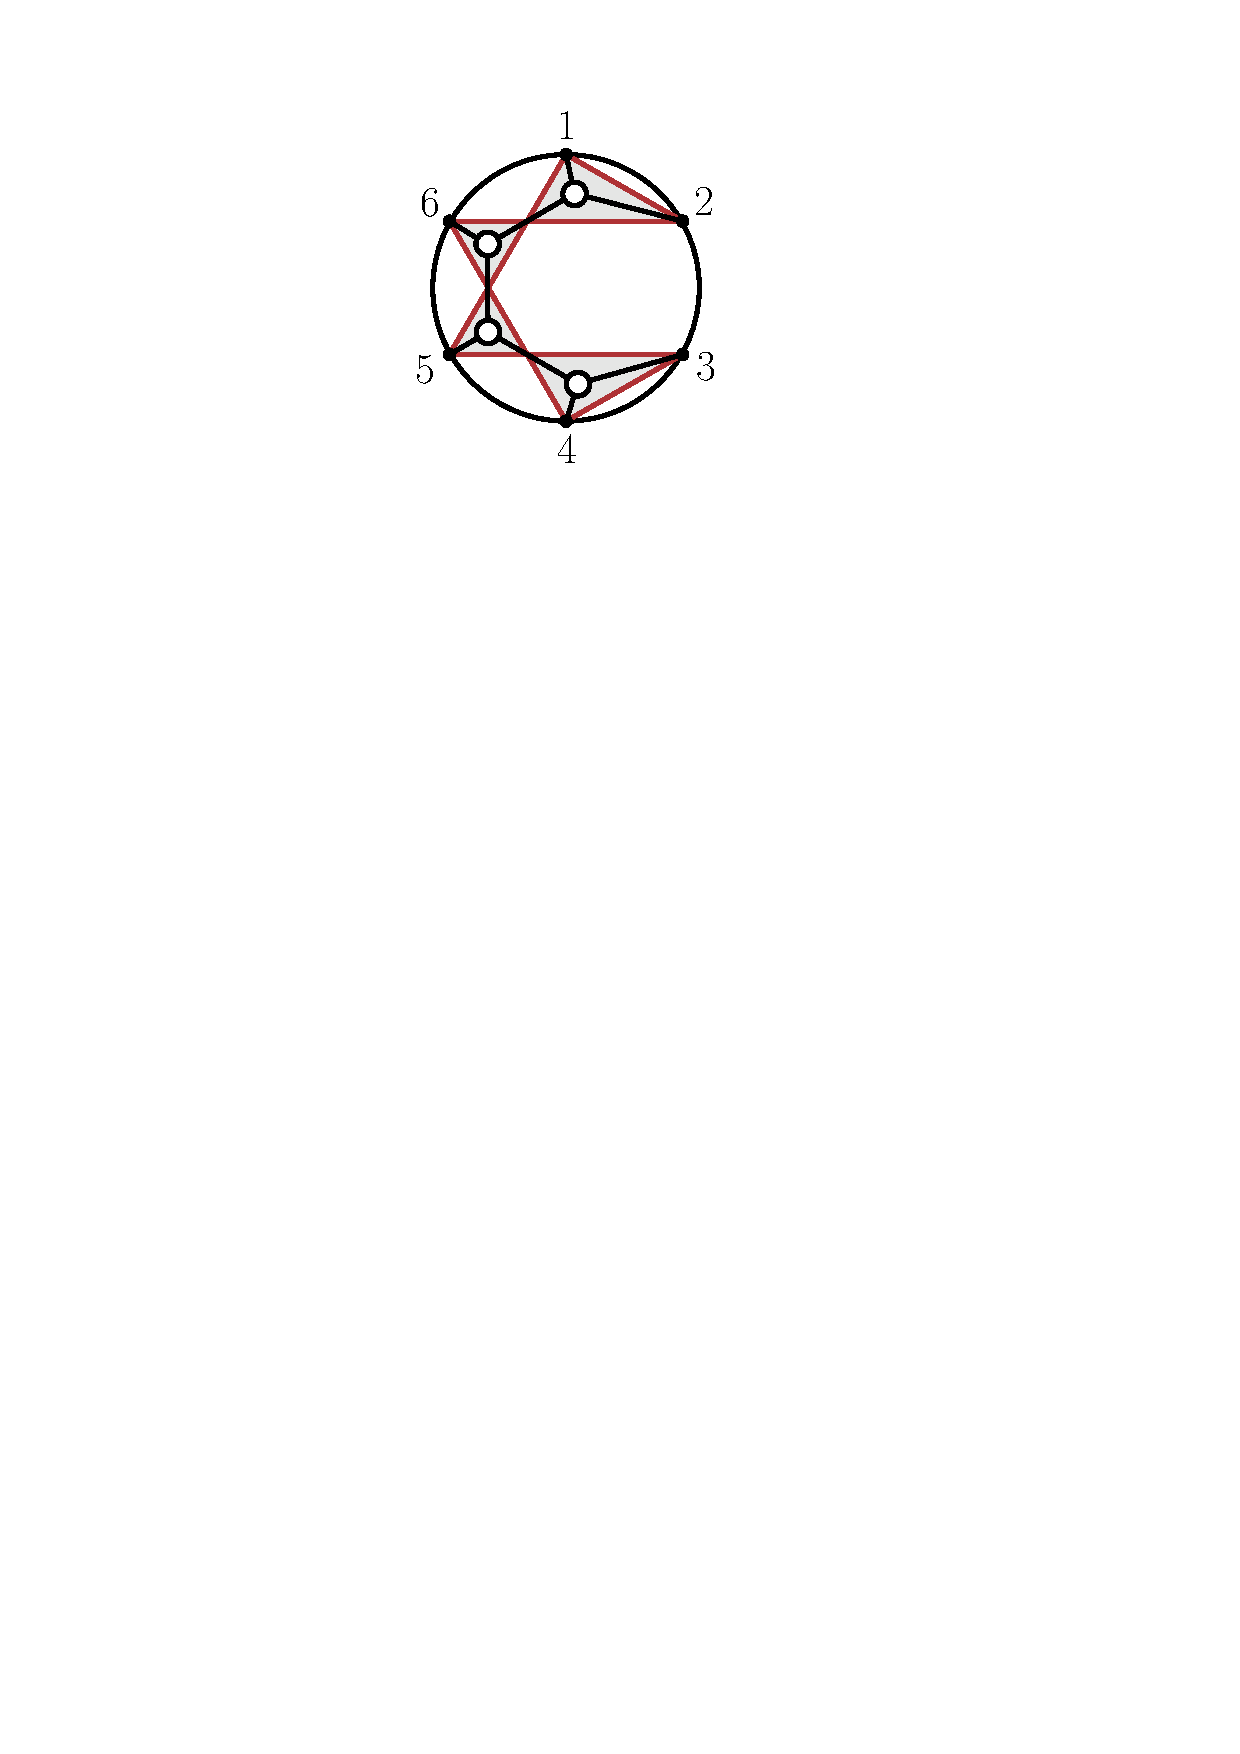
\includegraphics[scale=.5]{figs/eqfig1.pdf}} =\, \frac{1}{\sin s_{12} \,\sin s_{34} \,\sin s_{345}}
\end{equation}
\begin{equation}
\begin{aligned}
		m_{\alpha'}(\mathbb{I}_6|126345)\, &= \parbox[c]{6.5em}{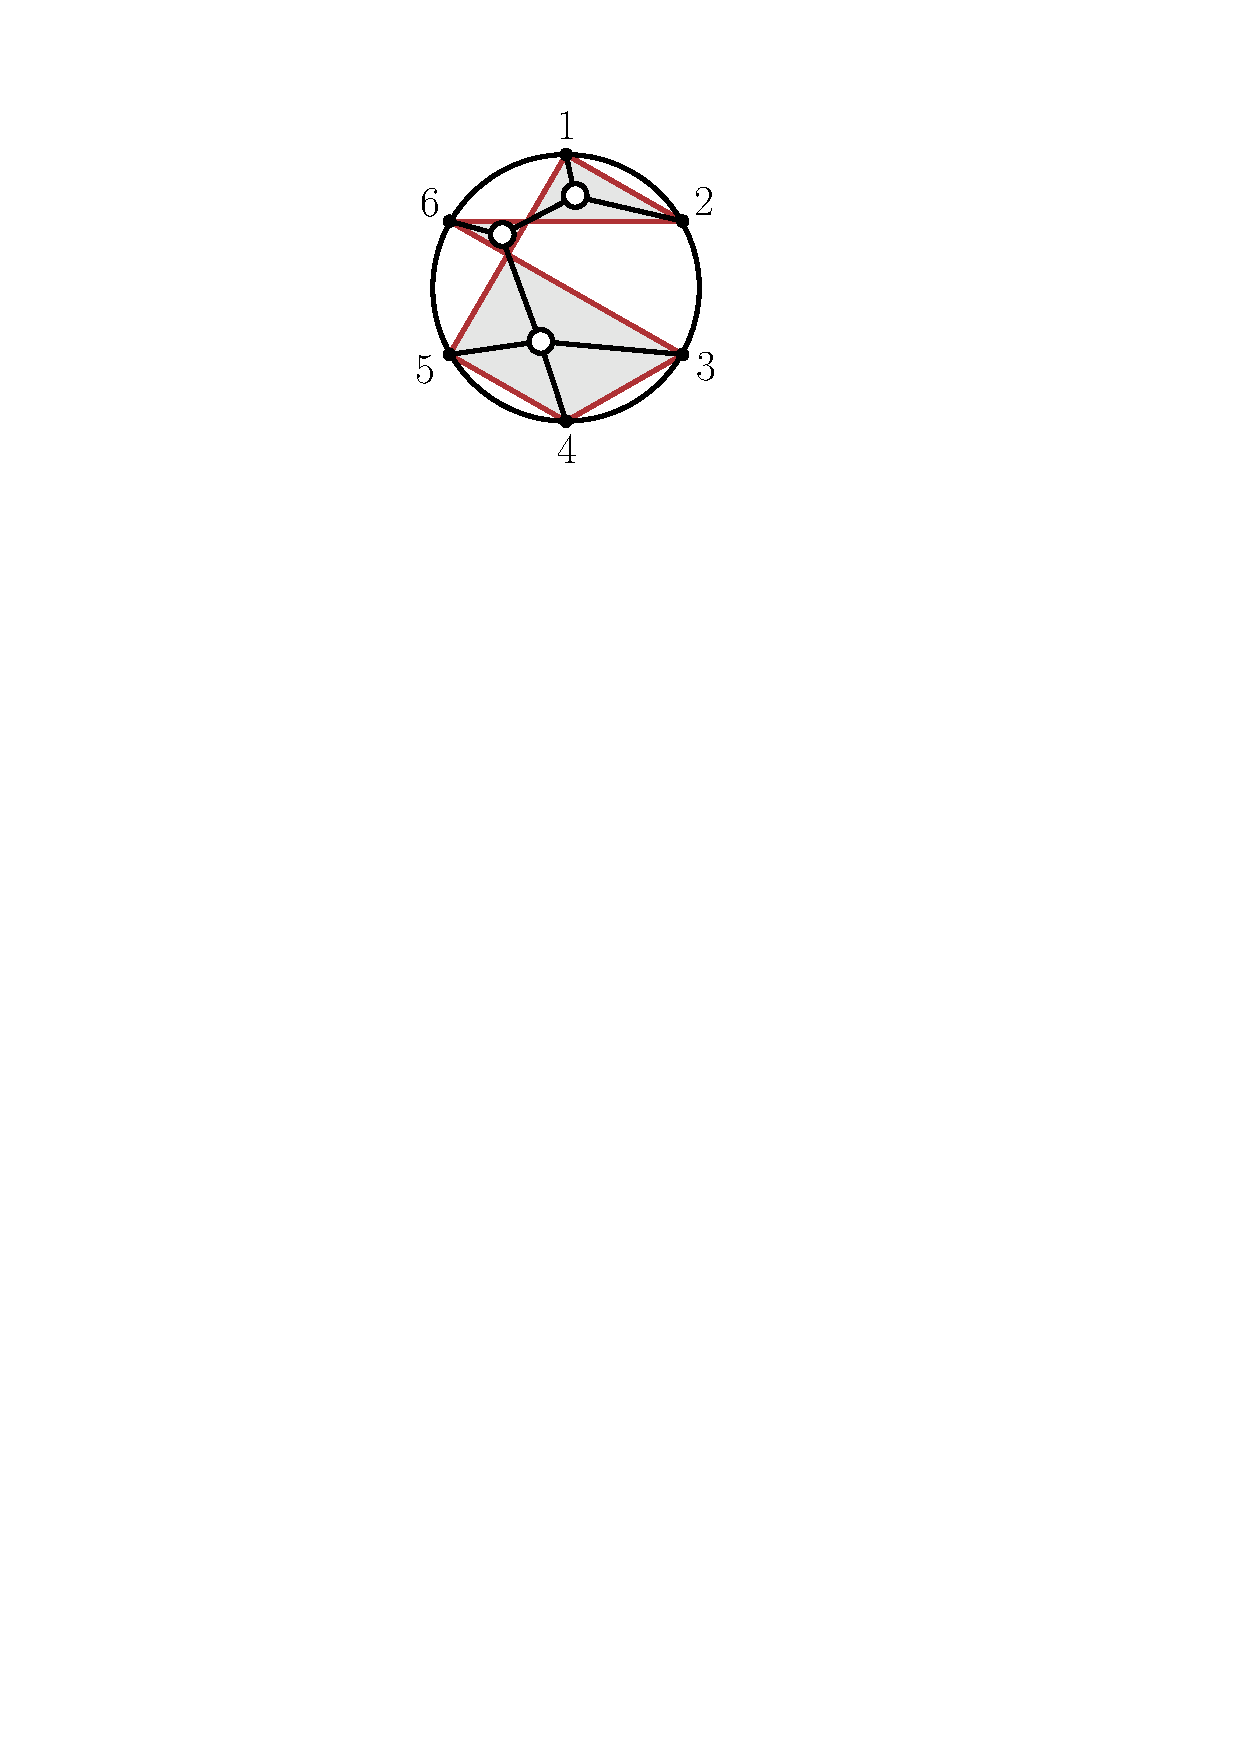
\includegraphics[scale=.5]{figs/m-123456-126345.pdf}} =\, -\frac{1}{\sin s_{12} \,\sin s_{612}} \times\!\!\! \parbox[c]{6.5em}{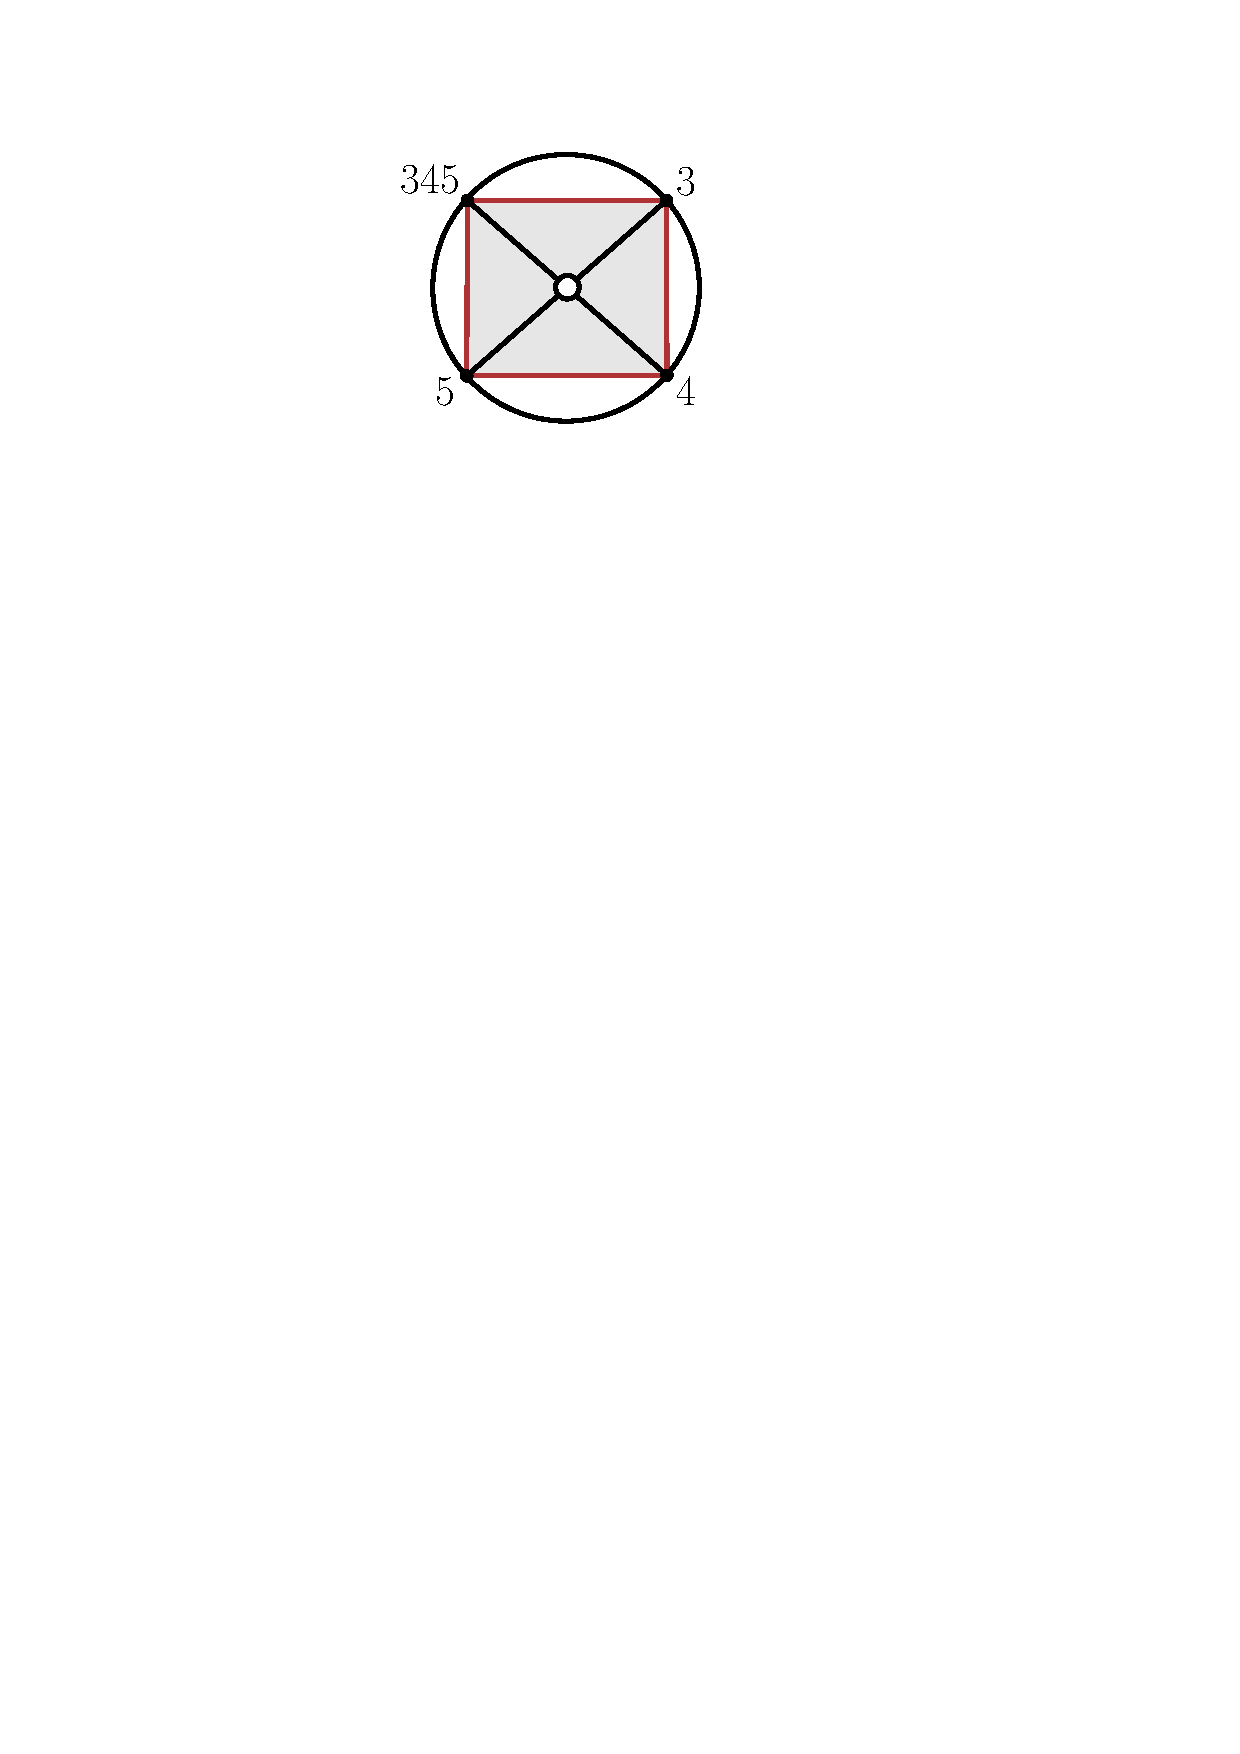
\includegraphics[scale=.5]{figs/m-123456-126345-small.pdf}}\\
	&=\, -\frac{1}{\sin s_{12} \,\sin s_{612}} \left(\frac{1}{\tan s_{34}} + \frac{1}{\tan s_{45}} \right)
\end{aligned}
\end{equation}

依赖上面两个式子我们来说明这一图形规则,首先计算$\alpha\neq\beta$,他们可以展开成$\alpha=\beta$的情况。展开方法就是先按照$\alpha$的顺序在盘面上把点标记出来,然后再按照$\beta$的顺序连接,也就是上图的红线,如果这一步给出的不是平面图,比如$m_{\alpha'}(12345|13524)$一样的五角星,那么就直接是$0$。这些红线会交出多边形,每个多边形内部画一个白点,白点之间连接,给出传播子$1/\sin(s_e)$,白点和多边形顶点相连,相当于动量外腿。每个多边形看作这种费曼规则的一个顶点,他们就贡献$m_{\alpha'}(\mathcal{E}|\mathcal{E})$,$\mathcal{E}$表示顶点边上动量外腿的集合。前面的正负号由缠绕数的计算给出$(-1)^{w(\alpha|\beta)+1}$:
\begin{equation}
	w(\mathbb{I}_6 | 126345)\, = \parbox[c]{6.5em}{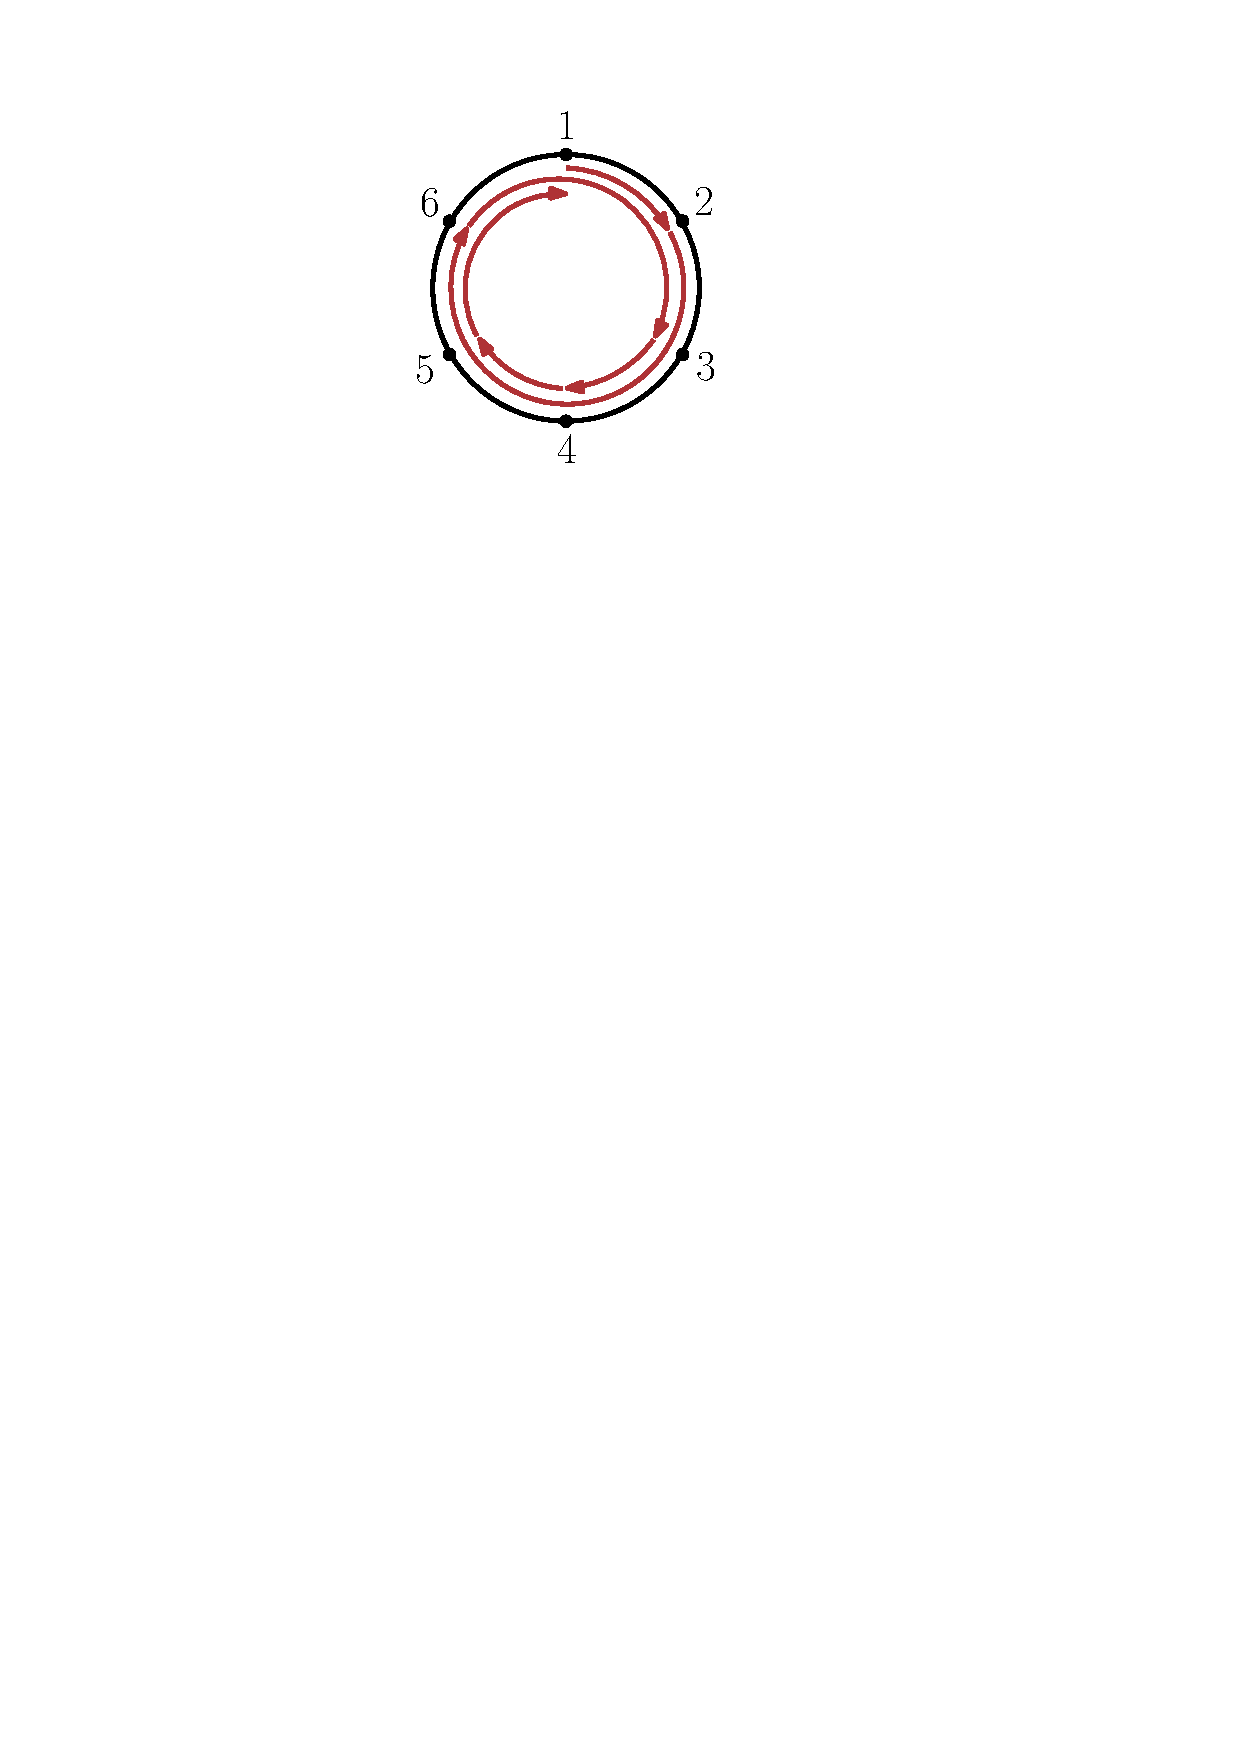
\includegraphics[scale=.5]{figs/wrapping.pdf}}\, =\, 2
\end{equation}
也就是说,缠绕数计算就是按照$\beta$的顺序缠绕$\alpha$得来。然后计算对角部分,也就是那些“顶点”项,以$\alpha=\beta=\mathbb{I}_n$为例,剩下的可以通过置换下标得到:
\begin{equation}
\begin{aligned}
		m_{\alpha'}(\mathbb{I}_5 | \mathbb{I}_5 )\, =\,& \parbox[c]{6.5em}{\vspace{-.5em}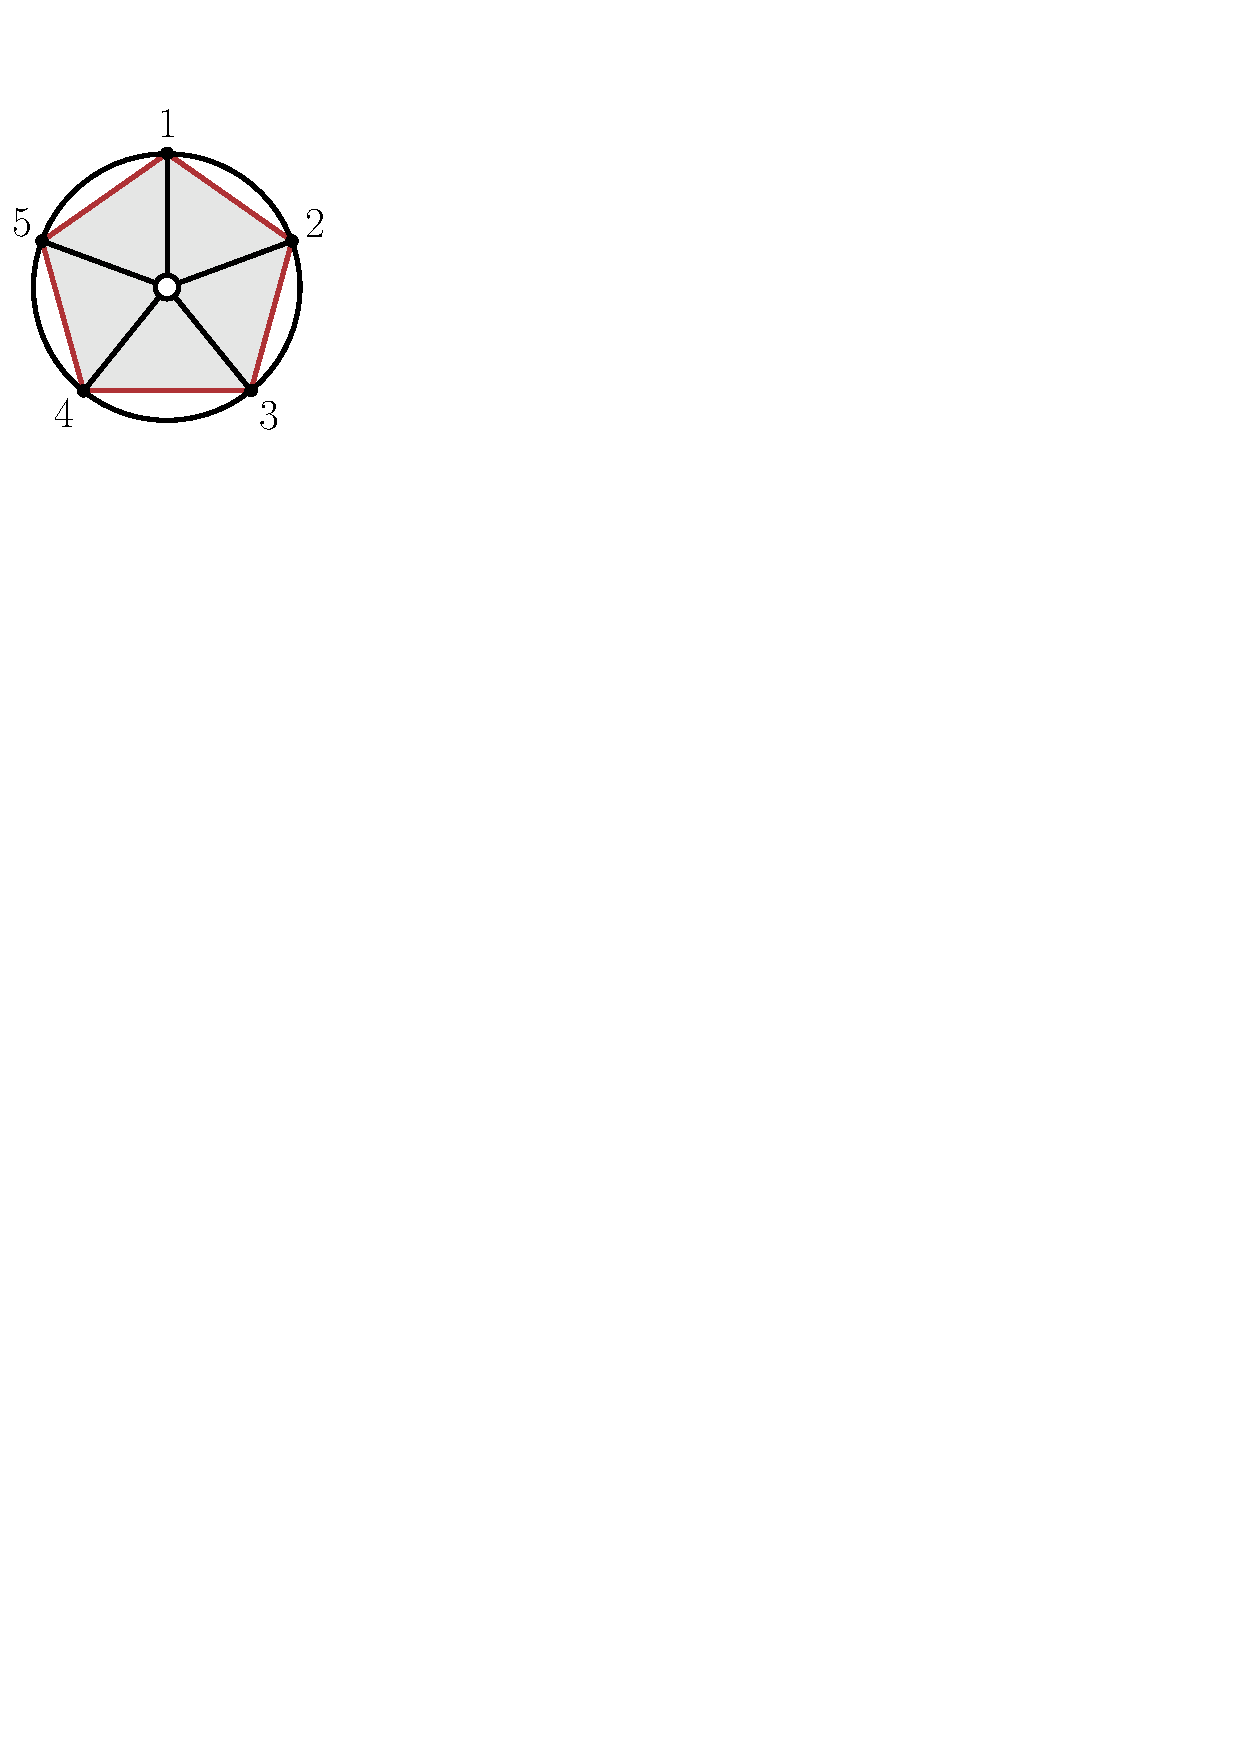
\includegraphics[scale=.5]{figs/m-12345-12345}}\, =\begin{aligned}
			\parbox[c]{6em}{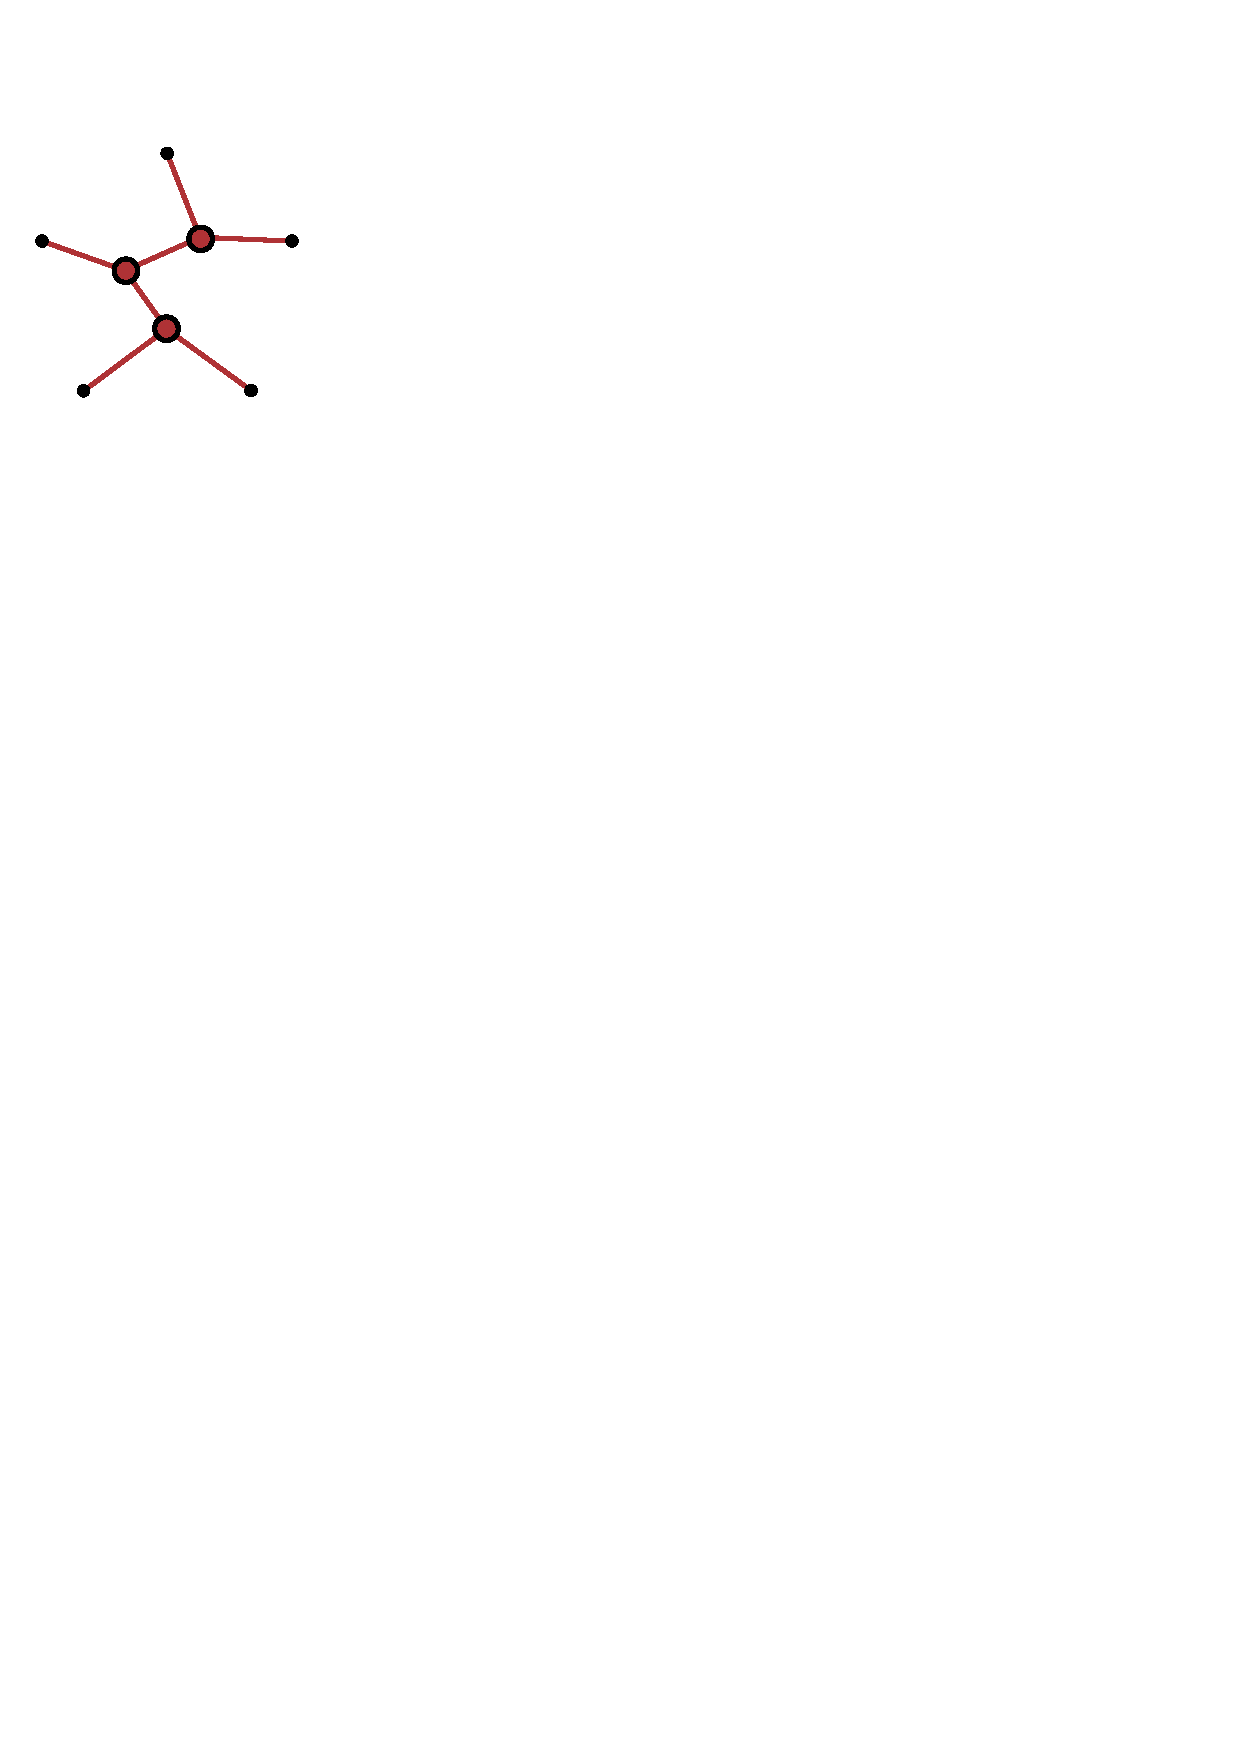
\includegraphics[scale=.5]{figs/m-12345-12345-a}}\, + \,\parbox[c]{6em}{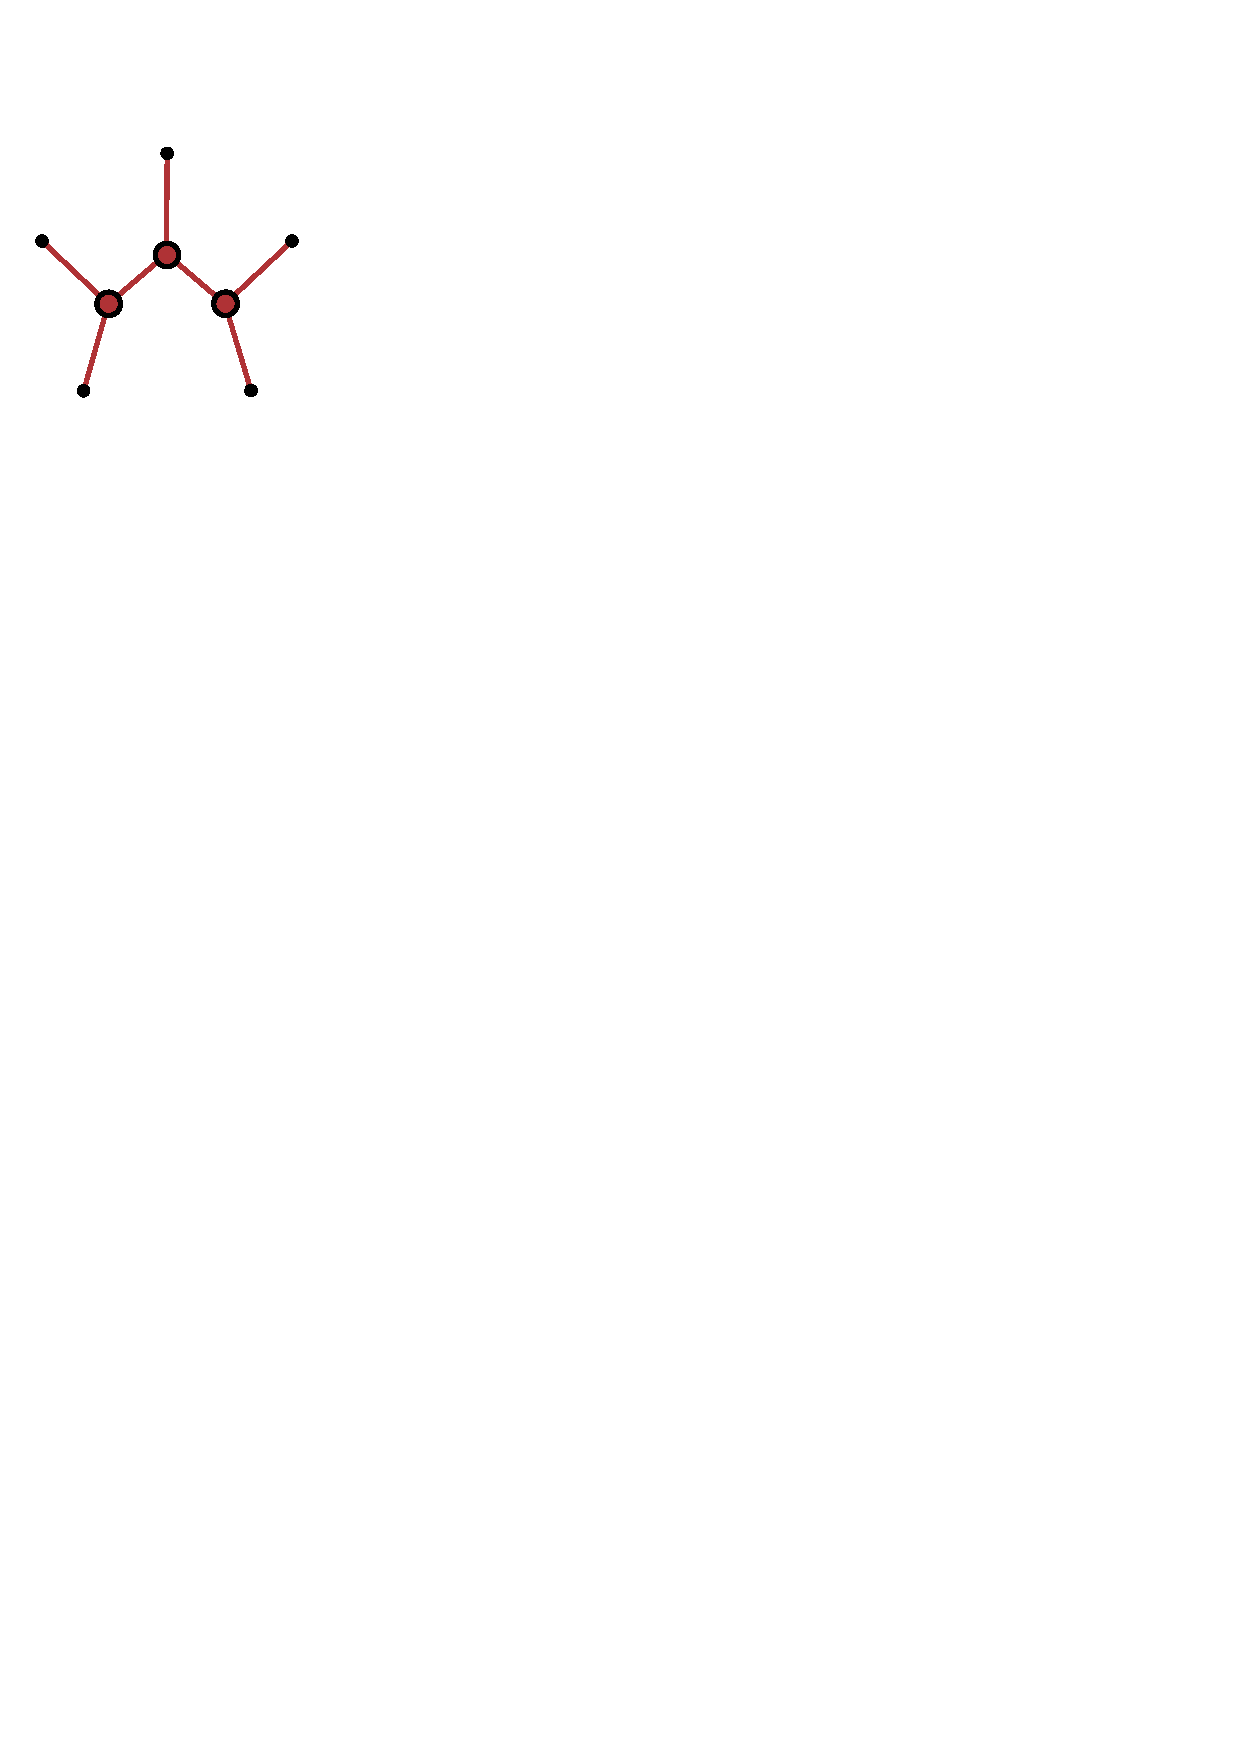
\includegraphics[scale=.5]{figs/m-12345-12345-b}}\, +\, \parbox[c]{6em}{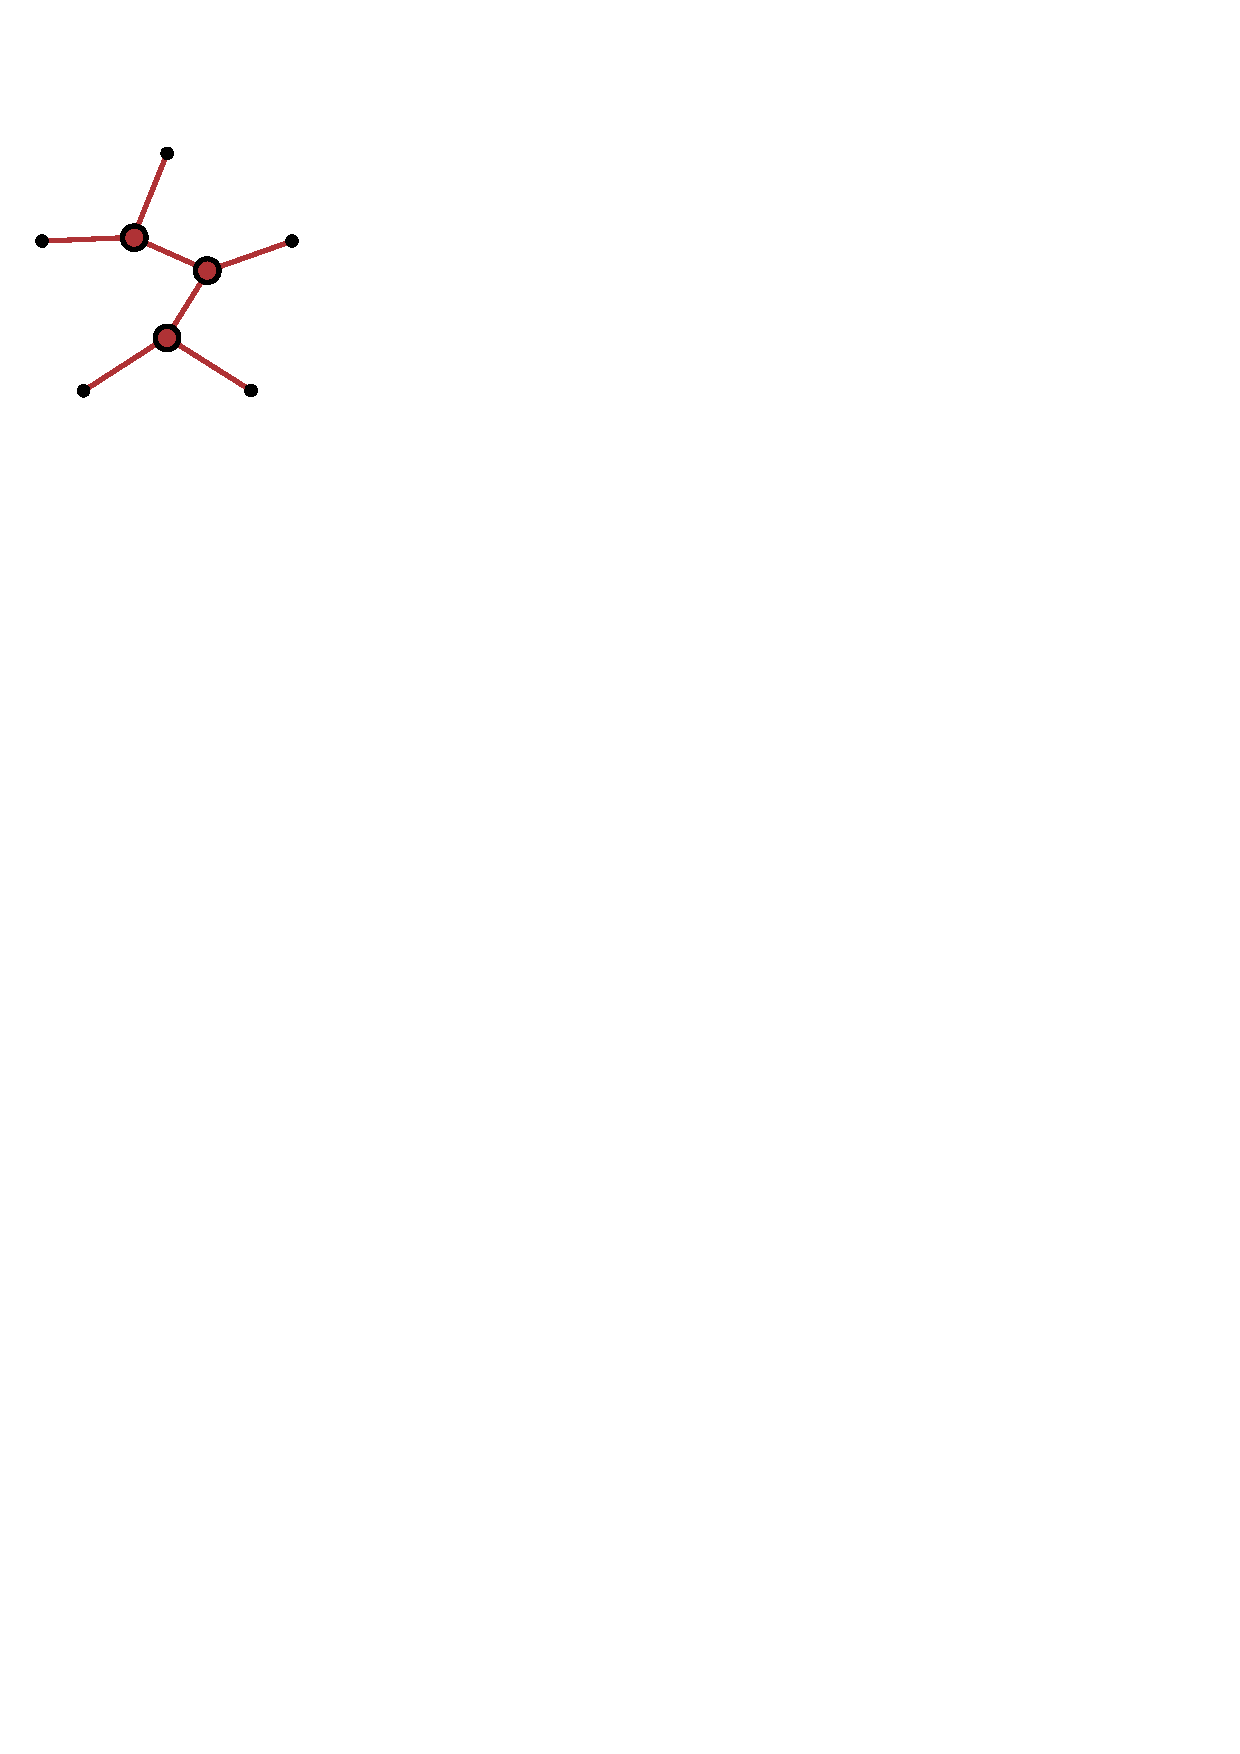
\includegraphics[scale=.5]{figs/m-12345-12345-c}} \\
			+\, \parbox[c]{6em}{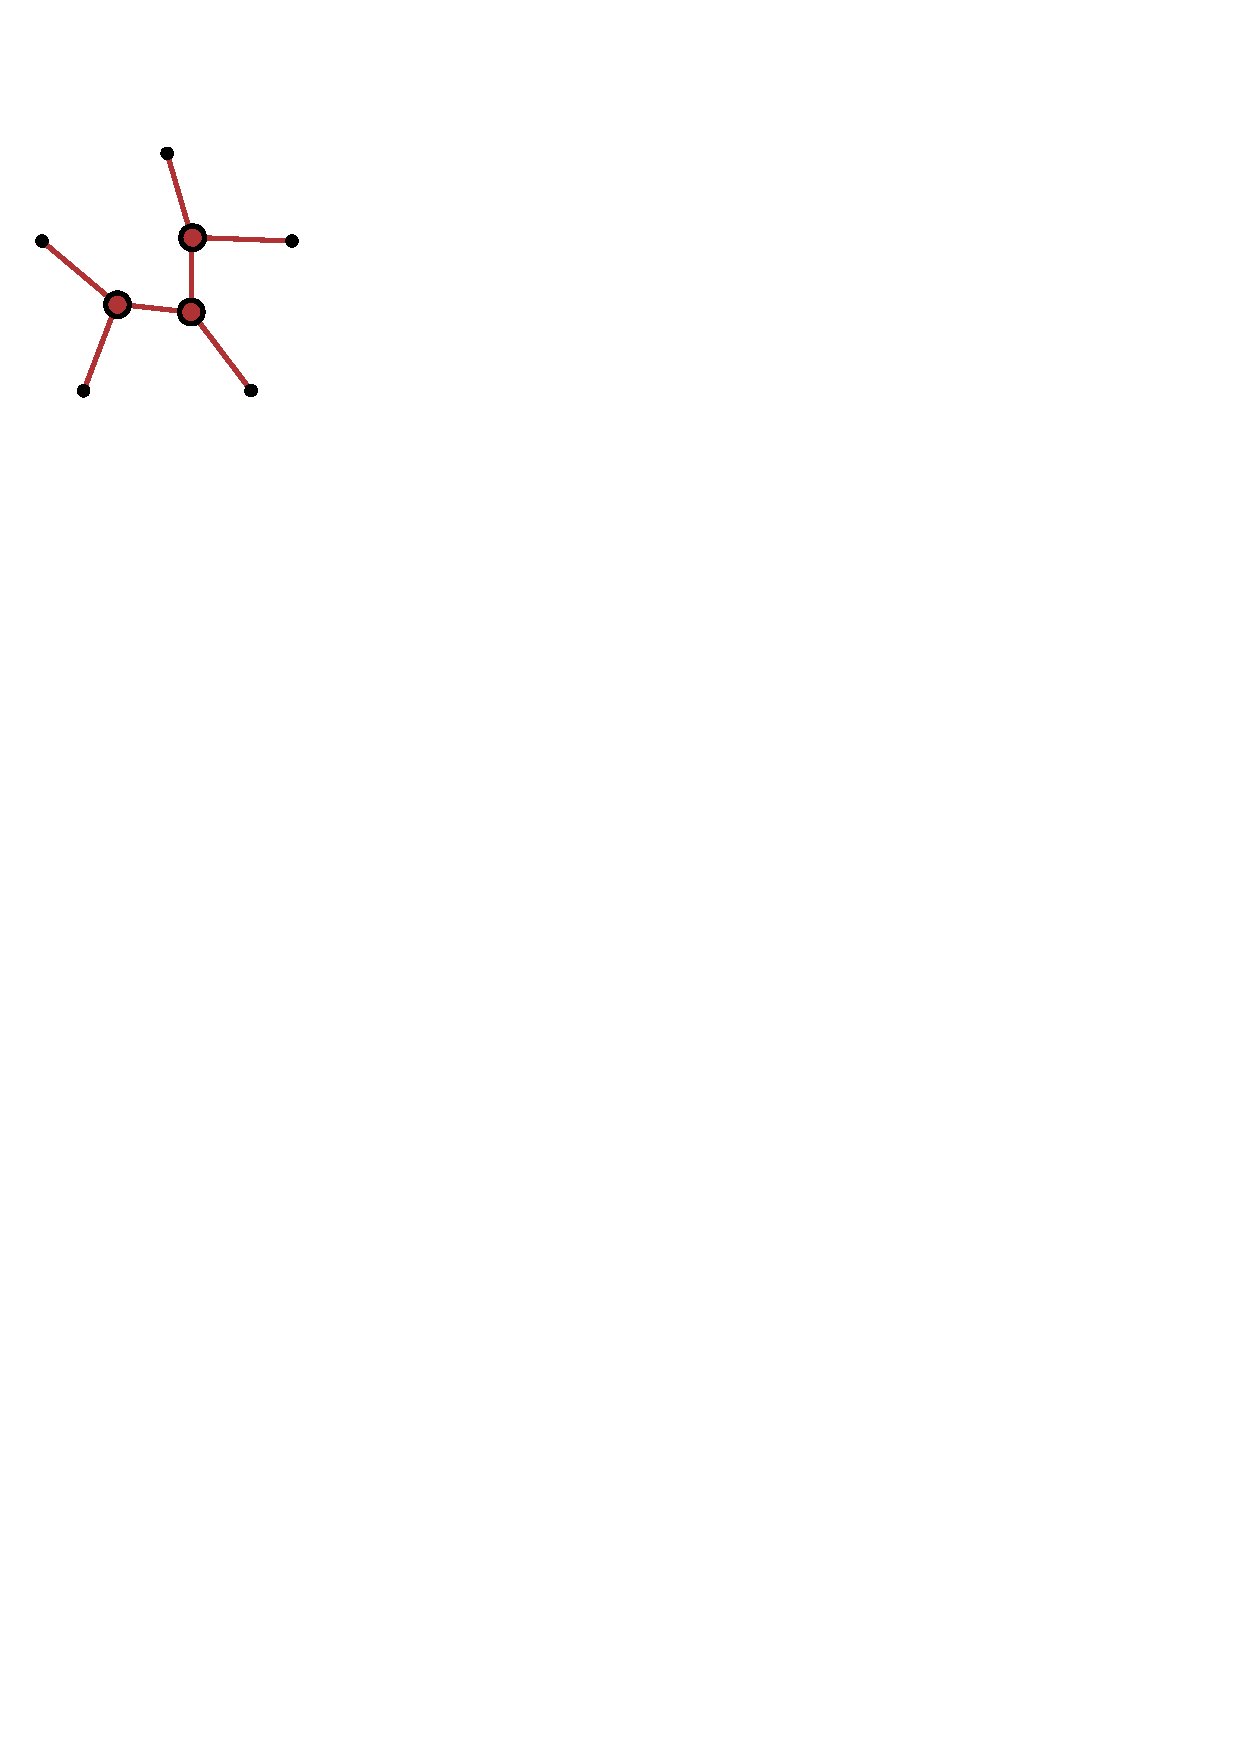
\includegraphics[scale=.5]{figs/m-12345-12345-d}}\, +\, \parbox[c]{6em}{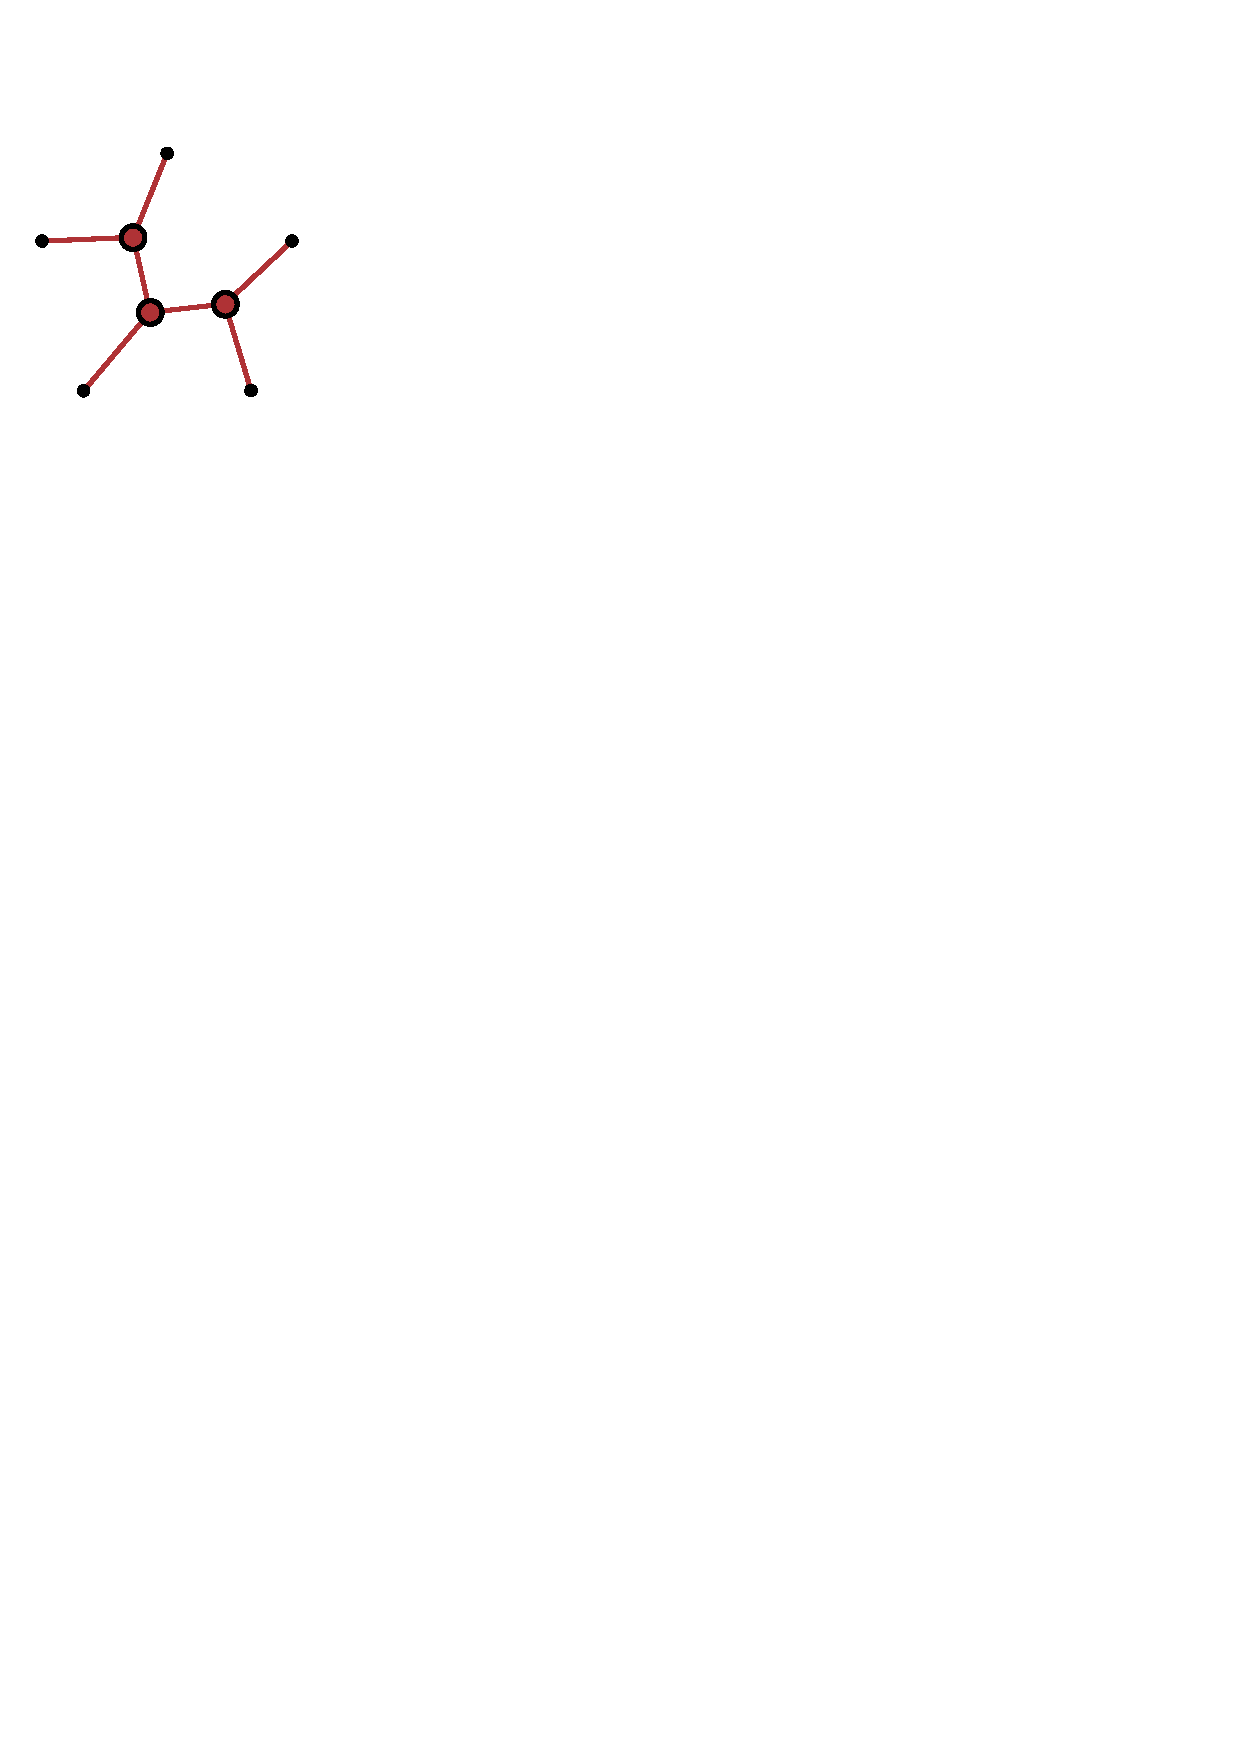
\includegraphics[scale=.5]{figs/m-12345-12345-e}} \,+\, \parbox[c]{6em}{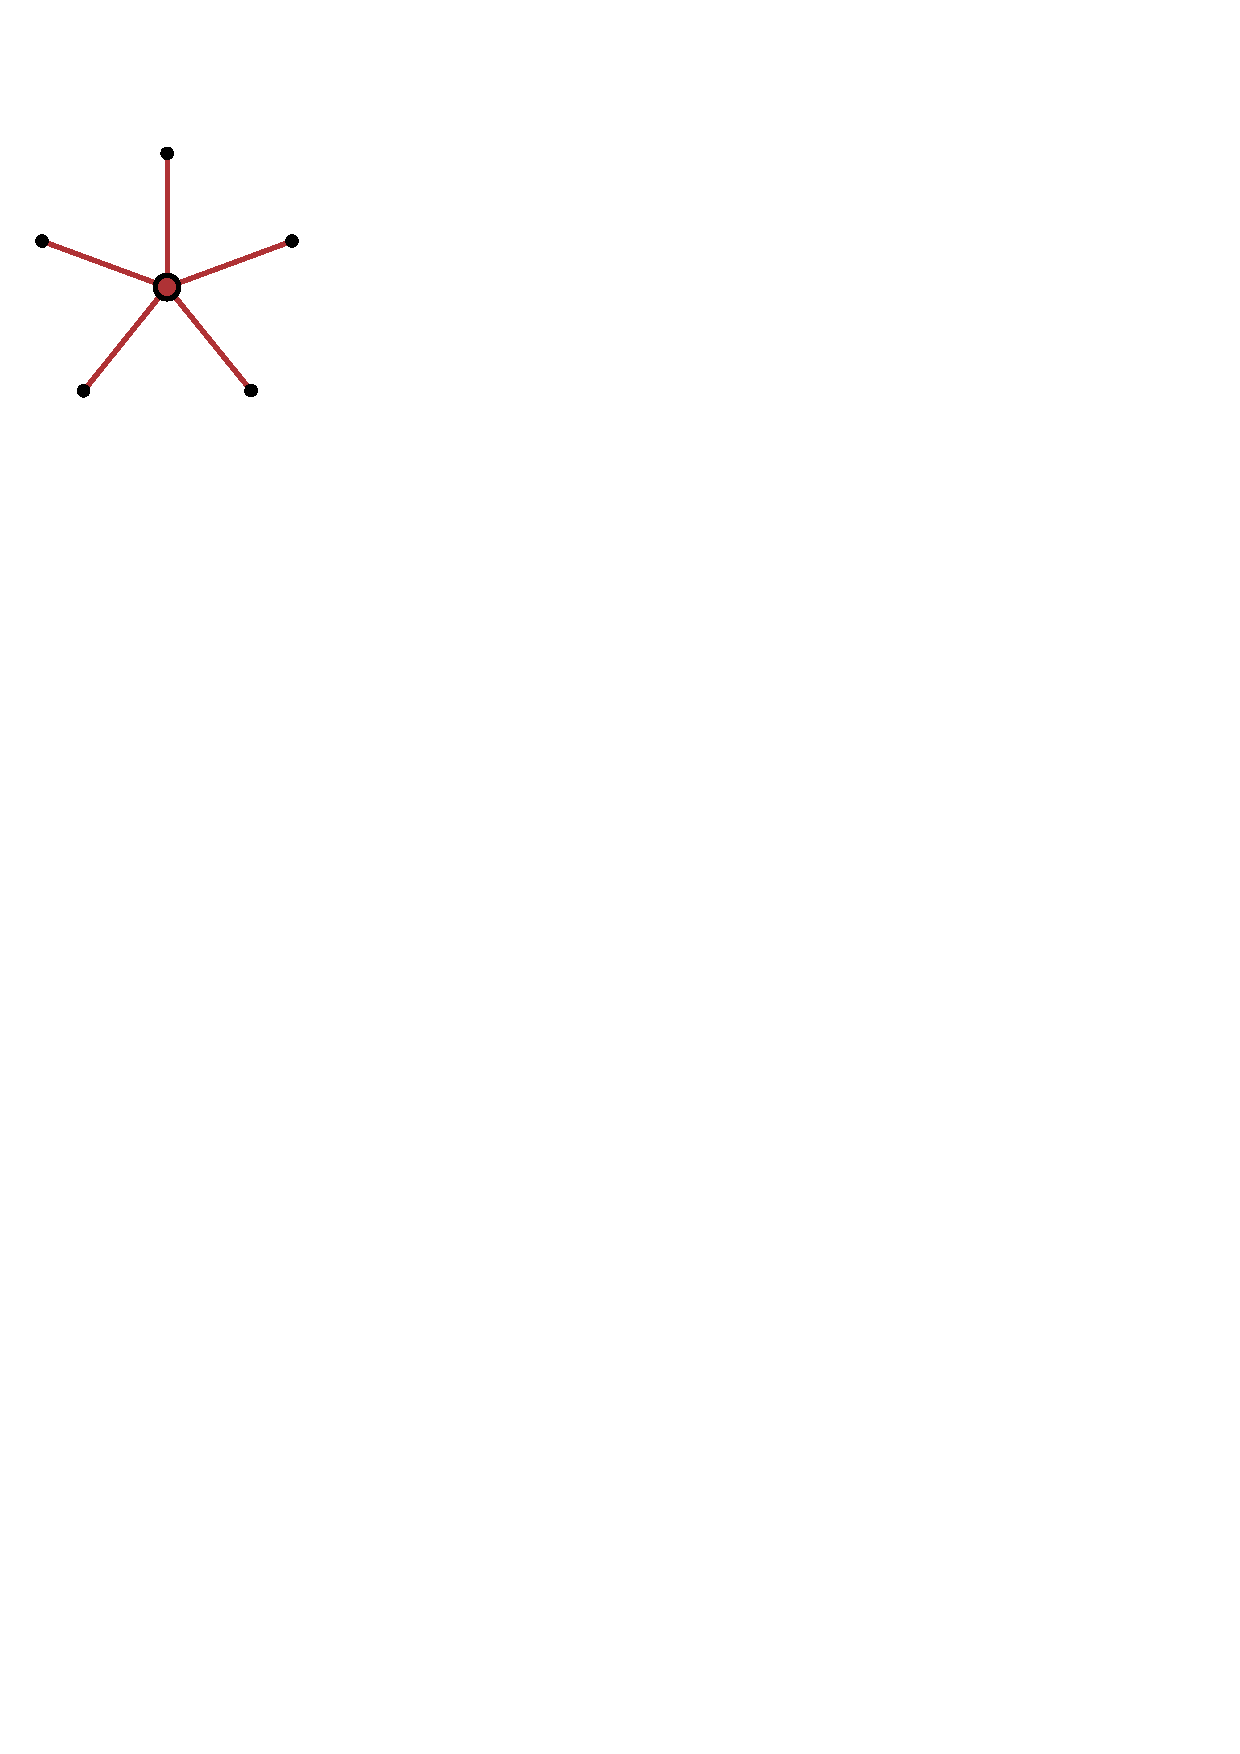
\includegraphics[scale=.5]{figs/m-12345-12345-f}} \\
		\end{aligned} \\
	=& \quad\frac{1}{\tan s_{12}\, \tan s_{34}} + \frac{1}{\tan s_{23}\, \tan s_{45}} + \frac{1}{\tan s_{34}\, \tan s_{51}} 
	 + \frac{1}{\tan s_{45}\, \tan s_{12}} \\
	 &+ \frac{1}{\tan s_{51}\, \tan s_{23}} + 1
\end{aligned}
\end{equation}
也就是说首先画出所有外腿顺序固定的所有用奇数外腿顶点构造的费曼图,每个顶点项贡献:
\begin{equation}
	\parbox[c]{8em}{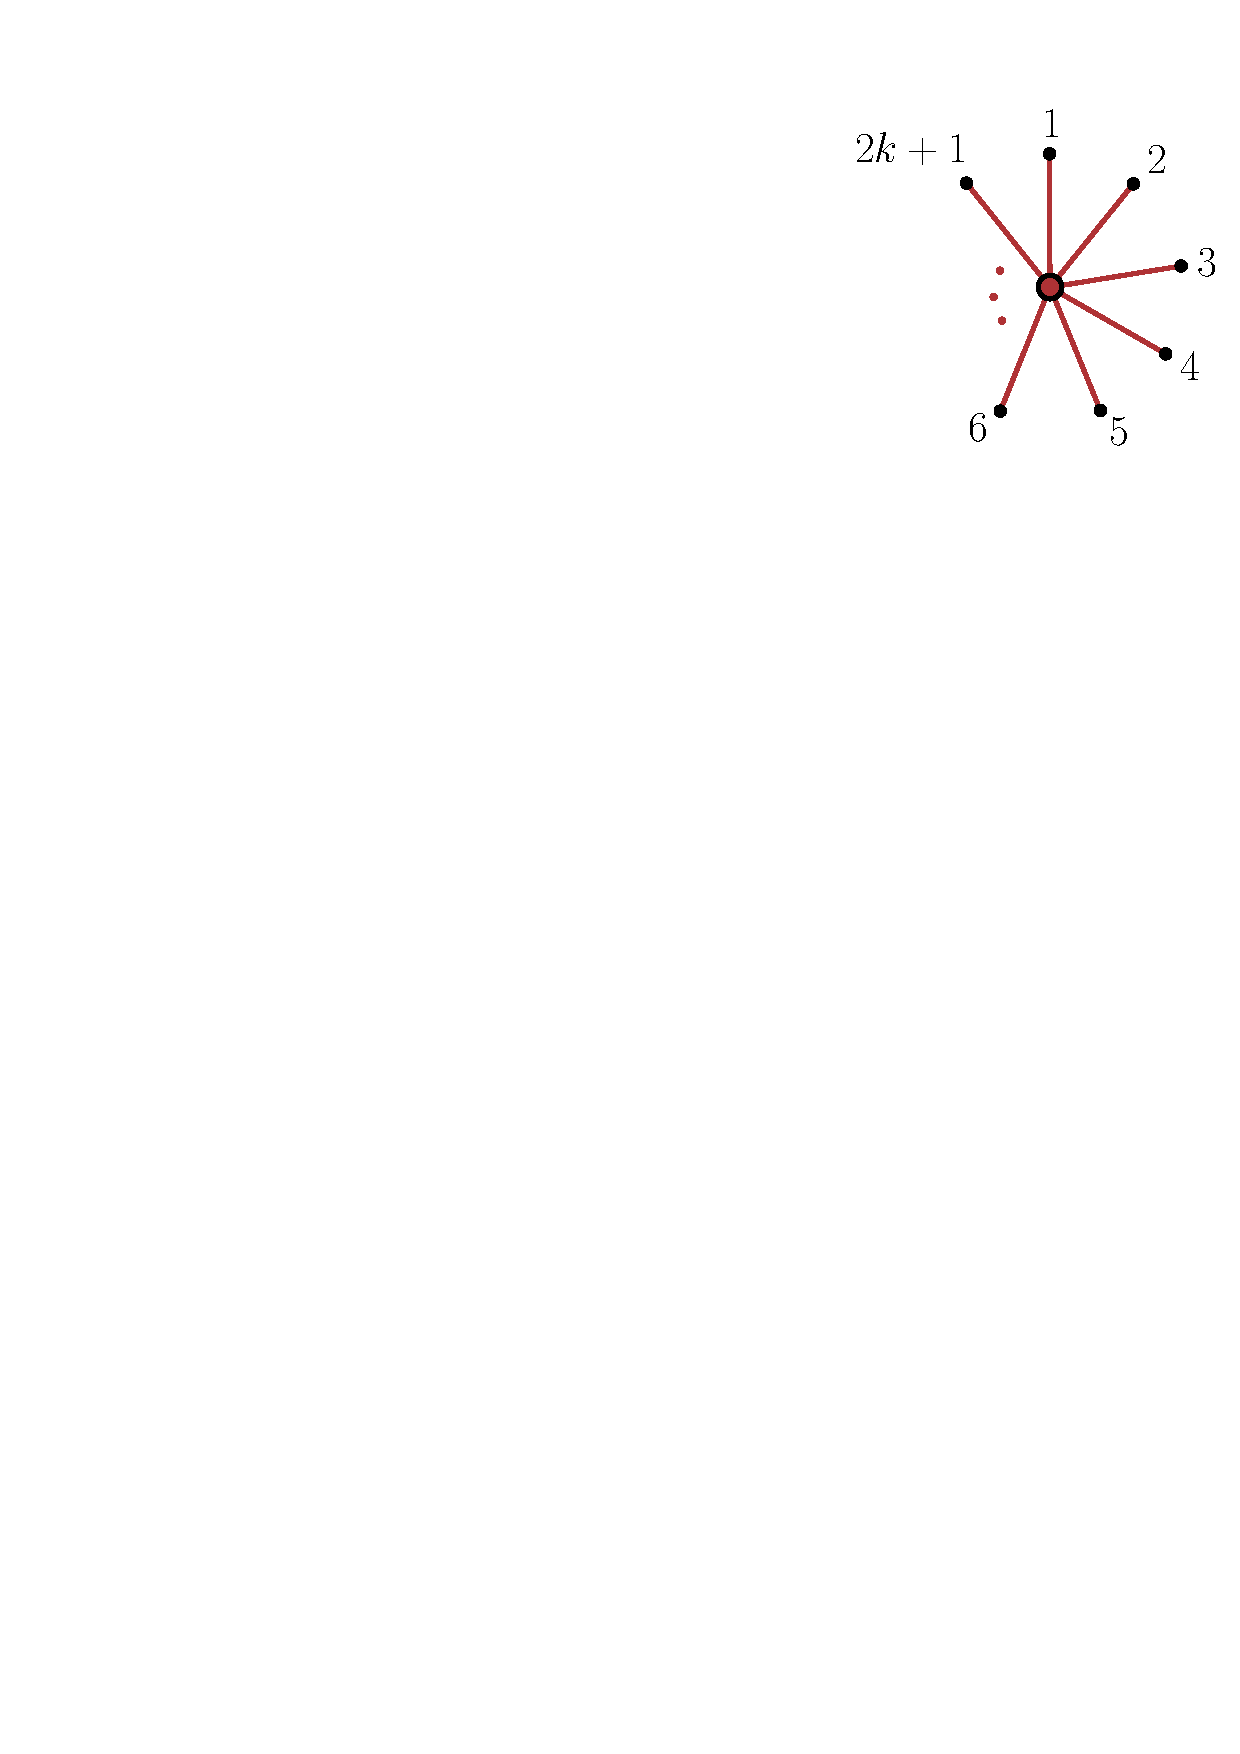
\includegraphics[scale=.5]{figs/m-vertex}}\; = \; C_{k-1}
\end{equation}
$C$是Catalan数。而每个传播子贡献$1/\tan(s_e)$。然后对$m_{\alpha'}$取逆矩阵就得到需要的KLT矩阵。上述色序振幅可以对应到一个场论,所以KLT关系实际上在说:
\begin{equation*}
	\text{Closed string}=\frac{\text{Open string}^2}{\alpha^{\prime}\text{-corrected bi-adjoint scalar}}
\end{equation*}

KLT关系实际上依赖于球面上左右模独立传播的特性,这一点在$\mathbb{RP}^2$上并不成立,所以无法分解为盘面振幅\cite{dyj}。文献\cite{Kawai:1985xq}中特别对四点情况KLT关系进行了详细论证。规范固定后四点KLT核只有一项,所以:
\begin{equation}
	\mathcal{M}_4 \sim-\frac{\sin(\pi s_{12})}{2\pi\alpha^{\prime}}A_4(1,2,3,4)\tilde A_4(1,2,4,3)
\end{equation}
不难发现这正是振幅\ref{Veneziano}和\ref{eq:4.45}之间的联系。\footnote{计算中需要用到$\sin(\pi x) = \frac{-\pi}{\Gamma(x+1)\Gamma(-x)}$。}
\section{RNS超弦振幅}
\subsection{自旋场关联函数}
在计算涉及R部分激发态时,会用到自旋场。回忆一下用OPE计算关联函数,首先用Wick定理计算多点OPE看出奇异性,而树图关联函数又只依赖于这种奇异性,所以可以直接用Wick收缩得到关联函数。但是,观察自旋场OPE,我们发现R部分并不是一个自由CFT,也就是说OPE得到的结果仍然包含场算符。对于非自由CFT,原先使用的Wick定理这些都失效了,本身关联函数相较于OPE也多了不少信息,但是,至少对于两个自旋场插入情况,我们可以利用OPE得知的关联函数奇异性信息完全从两点三点关联函数自举$n$点振幅。根据$\psi$和$S_A$都是共形主场,再根据他们的指标($SO(D-1,1)$表示)类型可以完全确定两点三点关联函数:
\begin{equation}
	\label{eq:4.61}
	\langle\psi^\mu(z_1)S_A(z_2)S_B(z_3)\rangle=\frac{(\Gamma^\mu\mathcal{C})_{AB}}{\sqrt{2}z_{12}^{1/2}z_{13}^{1/2}z_{23}^{D/8-1/2}},\quad \left\langle{S_{A}(z_1)S_{B}(z_2)}\right\rangle=\frac{\mathcal{C}_{AB}}{(z_1-z_2)^{D/8}}
\end{equation}
这是共形场论中熟知的结论,GSO投影将R部分真空投影到Weyl旋量,所以有如下的分解:\footnote{$\mathcal{C}_{AB}$的分解与时空维数有关,这里是$2\mod 4$的情况,而对$2\mod 4$,分解为$\mathcal{C}_{AB}=\begin{pmatrix}C_{\alpha\beta}&0\\0&C^{\dot{\alpha}\dot{\beta}}\end{pmatrix}$。}
\begin{equation}
	S_A=\begin{pmatrix}S_\alpha\\S^{\dot{\alpha}}\end{pmatrix},\quad(\Gamma^\mu)_A{}^B=\begin{pmatrix}0&\gamma_{\alpha\dot{\beta}}^\mu\\\bar{\gamma}^{\mu\dot{\alpha}\beta}&0\end{pmatrix},\quad \mathcal{C}_{AB}=\begin{pmatrix}0&{C_{\alpha}}^{\dot{\beta}}\\{C^{\dot{\alpha}}}_{\beta}&0\end{pmatrix}
\end{equation}
后面开弦计算只会用到其中一个手性,比如$S_\alpha$,$\gamma^\mu_{\alpha\dot\beta}$和$C_{\alpha}^{\dot\beta}$。我们以四点为例说明如何计算球面上的关联函数。首先根据其指标结构可以写下一般的拟设:
\begin{equation}
	\langle\psi^\mu(z_1)\psi^n(z_2)S_A(z_3)S_B(z_4)\rangle=\eta^{\mu\nu}\mathcal{C}_{AB}f(\mathbf{z})+\frac{1}{2}(\Gamma^\mu\Gamma^\nu\mathcal{C})_{AB}g(\mathbf{z})
\end{equation}
然后根据OPE领头阶得到如下奇异行为:
\begin{equation}
	\langle\psi^\mu(z_1)\psi^\nu(z_2)S_A(z_3)S_B(z_4)\rangle\to
	\begin{cases}\frac{\eta^{\mu\nu}}{z_m}\langle S_A(z_3)S_B(z_4)\rangle&, z_1\to z_2\\\frac{{{\Gamma^{\mu}}_A}^C}{\sqrt{2}z_{13}^{1/2}}\langle\psi^n(z_2)S_C(z_3)S_B(z_4)\rangle&, z_1\to z_3\\\frac{{{\Gamma^{\mu}}_B}^C}{\sqrt{2}z_{14}^{1/2}}\langle\psi^n(z_2)S_A(z_3)S_C(z_4)\rangle&, z_1\to z_4
	\end{cases}
\end{equation}
再利用关联函数\ref{eq:4.61}得到:
\begin{equation}
	\begin{aligned}
		&f(\mathbf{z})\to\begin{cases}z_{12}^{-1}z_{34}^{-D/8}&,z_1\to z_2\\\mathrm{regular}&,z_1\to z_3\\(z_{14}z_{23}z_{24})^{-1/2}z_{34}^{1/2-D/8}&,z_1\to z_4\end{cases}\\
		&g(\mathbf{z})\to\begin{cases}\mathrm{regular}&,z_1\to z_2\\(z_{13}z_{23}z_{24})^{-1/2}z_{34}^{1/2-D/8}&,z_1\to z_3\\(z_{14}z_{23}z_{24})^{-1/2}z_{34}^{1/2-D/8}&,z_1\to z_4\end{cases}
	\end{aligned}
\end{equation}
根据黎曼面上半纯函数都是有理形式,由上面奇异性直接得到:
\begin{equation}
	f(\mathbf{z})=\frac{z_{13}z_{24}}{z_{12}(z_{13}z_{14}z_{23}z_{24})^{1/2}z_{34}^{D/8}},\quad g(\mathbf{z})=\frac{1}{(z_{13}z_{14}z_{23}z_{24})^{1/2}z_{34}^{D/8-1}}
\end{equation}
从而有四点关联函数:
\begin{equation}
	\langle\psi^\mu(z_1)\psi^\nu(z_2)S_A(z_3)S_B(z_4)\rangle=\frac{z_{34}^{1-D/8}}{(z_{13}z_{14}z_{23}z_{24})^{1/2}}\left(\frac{z_{13}z_{24}}{z_{12}z_{34}}\eta^{\mu\nu}\mathcal{C}_{AB}+\frac{1}{2}(\Gamma^\mu\Gamma^\nu\mathcal{C})_{AB}\right)
\end{equation}
更高点的完全类似,只是拟设更为复杂,但是思想就是利用OPE读出奇异性,然后发现奇异性本身就足以和拟设一起完全确定关联函数。至于更高亏格以及更一般性的讨论详见文献\cite{Schlotterer:2012zz}及其所引文献。
\subsection{振幅的计算}
由于球面超弦振幅同样可以根据KLT关系用盘面超弦振幅表达,所以这里只计算一些简单的盘面超弦振幅。首先是三胶子振幅:
\begin{equation}
	\label{eq:4.71}
	\begin{aligned}
		A_3(\epsilon_1,\epsilon_2,\epsilon_3)=&|z_{12}z_{13}z_{23}|\langle U^{(0)}(z_1)U^{(-1)}(z_2)U^{(-1)}(z_3)\rangle\\
		\sim&|z_{12}z_{13}z_{23}|\langle:e^{-\phi(z_2)}::e^{-\phi(z_3)}:\rangle\epsilon_{1\mu}\epsilon_{2\nu}\epsilon_{3\lambda}\\
		&\times\left\{\left\langle :i\partial_{z_1}X^\mu(z_1)e^{ip_1\cdot X(z_1)}:\prod_{j=2}^3:e^{ip_j\cdot X(z_j)}: \right\rangle\left\langle\psi^\nu(z_2)\psi^\lambda(z_3)\right\rangle\right.\\
		&+2\alpha'\left\langle\prod_{j=1}^3:e^{ip_j\cdot X(z_j)}:\right\rangle p_{1\rho}\left\langle:\psi^\rho\psi^\mu(z_1):\psi^\nu(z_2)\psi^\lambda(z_3)\right\rangle\bigg\}\\
		\sim&\cancelto{-1}{\frac{|z_{12}z_{13}z_{23}|}{z_{12}z_{13}z_{23}}}\left[(p_2\cdot\epsilon_1)(\epsilon_2\cdot\epsilon_3)+(\epsilon_1\cdot\epsilon_2)(p_1\cdot\epsilon_3)-(\epsilon_1\cdot\epsilon_3)(p_1\cdot\epsilon_2)\right]\\
		=&A_{\mathrm{SYM}}(\epsilon_1,\epsilon_2,\epsilon_3)
	\end{aligned}
\end{equation}
注意这里$|z_{1,2,3}|/z_{1,2,3}$的项取$\pm1$和色序有关,另外一个$(132)$的色序给出$+1$\footnote{所以如果没有色序,其实三胶子振幅直接就是$0$,这对应QED中没有三光子顶点。}。其中玻色场关联函数已在\ref{eq:4.37}中给出,剩下的自由费米子关联函数直接用OPE计算全部外腿Wick缩并即可,比如:
\begin{equation}
\begin{aligned}
		\left\langle:\psi^\rho\psi^\mu(z_1):\psi^\nu(z_2)\psi^\lambda(z_3)\right\rangle 
	&=\wick{\left\langle:\c1\psi^\rho\c2\psi^\mu:\c1\psi^\nu\c2\psi^\lambda\right\rangle} +\wick{\left\langle:\c1\psi^\rho\c2\psi^\mu:\c2\psi^\nu\c1\psi^\lambda\right\rangle} \\
	&=\frac{\eta^{\mu\nu}\eta^{\rho\lambda}-\eta^{\mu\lambda}\eta^{\rho\nu}}{z_{12}z_{13}}
\end{aligned}
\end{equation}
这里$A_{\text{SYM}}$表示十维超对称Yang-Mills理论的色序振幅,由下面拉格朗日量计算,$C$是荷共轭矩阵,$[D_\mu,\chi]:=\partial_\mu\chi-[A_\mu,\chi]$:
\begin{equation}
	S_{\mathrm{SYM}}[A,\chi]\sim\int d^{10}X\operatorname{Tr}\left\{\frac{1}{4}F_{\mu\nu}F^{\mu\nu}+\chi^\alpha(\gamma^\mu C)_{\alpha\beta}[D_\mu,\chi^\beta]\right\}
\end{equation}
再比如一个胶子两个胶伴子的振幅:
\begin{equation}
	\begin{aligned}
		A_3(\epsilon_{1},u_{2},u_{3})\sim&|z_{12}z_{13}z_{23}|\langle U^{(-1)}(z_{1})U^{(-1/2)}(z_{2})U^{(-1/2)}(z_{3})\rangle\\
		=&|z_{12}z_{13}z_{23}|\langle:e^{-\phi(z_1)}::e^{-\phi(z_2)/2}::e^{-\phi(z_3)/2}:\rangle\langle\prod_{j=1}^3:e^{ip_j\cdot X(z_j)}:\rangle\\
		&\times\epsilon_1^\mu u_2^\alpha u_3^\beta\langle\psi_\mu(z_1)S_\alpha(z_2)S_\beta(z_3)\rangle\\
		\sim&\cancelto{-1}{\frac{|z_{12}z_{13}z_{23}|}{z_{12}z_{13}z_{23}}}\frac{1}{\sqrt{2}}\epsilon_1^\mu(u_2\gamma_\mu C u_3)\\
		=&A_{\text{SYM}}(\epsilon_1,u_2,u_3)
	\end{aligned}
\end{equation}

原则上来说,超对称理论的振幅应当是用格拉斯曼变量编码得到的超振幅,比如四维$\mathcal{N}=4$ SYM理论,超多重态自由度可以用格拉斯曼变量$\eta$编码到同一个波函数中表示,而分量振幅就根据超振幅的格拉斯曼变量次数来确定,比如:
\begin{equation}
\begin{gathered}
		A_n\left[S^{12}S^{34}3^-4^+\ldots n^+\right]=\left(\frac{\partial}{\partial\eta_{11}}\frac{\partial}{\partial\eta_{12}}\right)\left(\frac{\partial}{\partial\eta_{23}}\frac{\partial}{\partial\eta_{24}}\right)\left.\left(\prod_{A=1}^4\frac{\partial}{\partial\eta_{3A}}\right)\mathcal{A}_n[\Omega_1,\ldots,\Omega_n]\right|_{\eta_{kC}=0}\\
	\Omega=g^++\eta_A\lambda^A-\frac{1}{2!}\eta_A\eta_BS^{AB}-\frac{1}{3!}\eta_A\eta_B\eta_C\lambda^{ABC}+\eta_1\eta_2\eta_3\eta_4g^-
\end{gathered}
\end{equation}

因为胶子与胶伴子共同构成一个超多重态,而前面计算那些振幅都应当是整个超振幅的某个分量振幅。但是由于RNS形式没有靶空间超对称,所以没办法直接计算超振幅。而且从前面三点振幅计算也能看出,超弦振幅和SYM振幅之间无论取外腿为超多重态中的哪一个态(胶子/胶伴子),振幅之间的关系是不变的。而纯旋量超旋顶角算符直接对超多重态定义,所以可以直接计算得到超振幅,后面我们会用纯旋量超弦形式将任意多点盘面超弦超振幅表达为SYM超振幅。

另外对比玻色弦胶子振幅\ref{eq:4.47}和超弦胶子振幅\ref{eq:4.71},发现超弦振幅竟然更加简单,少了$\propto\alpha'$的项。缺少某一项从低能场论上看相当于低能场论缺少某个相互作用顶点。在场论中,超对称的引入一般能较好地改善理论的紫外行为,体现在超对称会直接否定某些抵消项的存在,比如在七圈以下修正,$\mathcal{N}=8$超引力只允许存在抵消项$R^4$,$D^4R^4$,$D^6R^4$\cite{Elvang:2015rqa}。这也是超弦振幅更加简单一些的一种解释。

	\chapter{Berkovits超弦}
本节介绍靶空间超对称的纯旋量超弦,由Berkovits在2000年发现\cite{Berkovits:2000fe}。从历史上看最早试图从靶空间超对称引入超弦的形式是Green-Schwarz超弦\cite{Green:1983wt,Green:1983sg},但是只能在非协变的光锥坐标下量子化。后来Siegle改进了这一形式但存在共形反常且与RNS形式不等价等诸多问题\cite{Siegel:1985xj}。Berkovits在Siegle的研究基础之上进行改进得到了纯旋量超弦。我们不打算沿用历史性的介绍\cite{Berkovits:2002zk,Mafra:2008gkx},而改用自上而下的方式。本章首先从更简单的超对称点粒子模型出发,然后推广得到纯旋量超弦的作用量,更多细节详见\cite{Berkovits:2017ldz,Mafra:2022wml}。

\section{Brink-Schwarz 超粒子}
本节目的是说明在引入靶空间旋量进行超对称化,会导致体系无法协变量子化,以更简单的点粒子模型来说明,弦论类似。靶空间超对称粒子作用量:\cite{Brink:1981nb,Ferber:1977qx}
\begin{equation}
	\label{eq:5.1}
	S_{\text{BS}}=\int d\tau\left(\Pi^\mu P_\mu+eP^\mu P_\mu\right),\quad\Pi^\mu:=\dot{X}^\mu-\frac{1}{2}\dot{\theta}^\alpha\gamma_{\alpha\beta}^\mu\theta^\beta
\end{equation}
这里旋量都是十维靶空间旋量,选取了Weyl基底\ref{eq:4.65},$P$是$X$共轭动量,且看作独立变量。$\mathcal{N}=1$超对称以及对应的超荷为:
\begin{equation}
	\label{eq:5.2}
	\begin{gathered}
		\delta\theta^\alpha=\epsilon^\alpha,\quad\delta X^\mu=\frac{1}{2}\theta^\alpha\gamma_{\alpha\beta}^\mu\epsilon^\beta,\quad\delta P^\mu=\delta e=0\\
		Q_\alpha:=p_\alpha-\frac{1}{2}\gamma_{\alpha\beta}^\mu\theta^\beta P_\mu,\quad p_\alpha:=\frac{\partial L}{\partial\dot{\theta}^\alpha}=-\frac{1}{2}\gamma_{\alpha\beta}^\mu\theta^\beta P_\mu
	\end{gathered}
\end{equation}
这一作用量其实是GS形式弦理论的无质量点粒子极限,GS形式下有额外的格拉斯曼奇的规范对称性,称为$\kappa$对称性:
\begin{equation}
	\delta\theta^\alpha=P^\mu\gamma_\mu^{\alpha\beta}\kappa_\beta,\quad\delta X^\mu=-\frac{1}{2}\theta^\alpha\gamma_{\alpha\beta}^\mu\delta\theta^\beta,\quad\delta P^\mu=0,\quad\delta e=\dot{\theta}^\alpha\kappa_\alpha
\end{equation}
再来看下该体系的约束,首先是$\delta S/\delta e$给出$P^2=0$的无质量约束,这类似前面能动张量给出的约束。另外引入了两对共轭变量$\{X,P\}$和$\{\theta,p\}$,前面一对可以看作是独立的,但是从$\ref{eq:5.2}$不难看出$p$的定义本身包含$\theta$,所以并不能看作完全独立,而是要求有下面的约束条件:
\begin{equation}
	d_\alpha:=p_\alpha+\frac{1}{2}\gamma_{\alpha\beta}^\mu\theta^\beta P_\mu=0
\end{equation}
利用共轭变量之间的泊松括号得到约束条件满足的代数结构:
\begin{equation}
	\label{eq:5.4}
	\{d_\alpha,d_\beta\}_{\mathrm{PB}}=-\gamma_{\alpha\beta}^\mu P_\mu
\end{equation}
对于无质量粒子取小群表示$P^\mu=(E,0,\ldots,E)$,并且取$X,P,\gamma$的光锥坐标得到:
\begin{equation}
	\label{eq:5.5}
	\{d_\alpha,d_\beta\}_{\mathrm{PB}}=-\gamma_{\alpha\beta}^-P^+\propto\begin{pmatrix}{1}_{8\times8}&{0}_{8\times8}\\{0}_{8\times8}&{0}_{8\times8}\end{pmatrix}
\end{equation}
由此发现\ref{eq:5.4}给出的约束条件包含八个第一类约束和八个第二类约束,而且只有在不协变的光锥规范下,两类约束才不会混合在一起。所以GS形式只能在光锥坐标下进行量子化。

第一类约束比如前面玻色弦和RNS超弦量子化中能动张量给出的约束可以在协变量子化框架中将约束看作是\ref{eq:2.23}来解决,但是第二类约束需要用到$\S$\ref{sec:5.2}中的式\ref{2nd}先替换掉泊松括号,然后再进行正则量子化。下面我们直接选取规范固定将第一类约束解除,然后处理第二类约束。

在光锥规范下可以固定$\kappa$规范对称性为$(\gamma^+\theta)_\alpha=0$,在这一规范固定下,作用量\ref{eq:5.1}改写为:\footnote{计算需要利用靶空间Majorana-Weyl旋量性质$\dot{\theta}\gamma^+\theta=\dot{\theta}\gamma^i\theta=0$。}
\begin{equation}
S_{\text{BS}}=\int d\tau\left(\dot{X}^\mu P_\mu-\frac{1}{2}\dot{S}_aS_a+eP^\mu P_\mu\right),\quad S^a:=2^{1/4}\sqrt{P^+}\theta^a
\end{equation}
这里利用了十维Weyl旋量可以进一步分解为Weyl和反Weyl旋量,$\theta$规范固定后还剩下一半的分量:\footnote{这是将十维Weyl旋量分解为了两个八维Weyl旋量,而且八维Weyl旋量升降指标的度量矩阵是$\delta^{ab}$单位阵,一般情况下利用荷共轭矩阵的分量来升降指标\cite{Freedman:2012zz},比如四维情况下一般取基底使得升降矩阵为Levi-Civita张量$\varepsilon^{ab}$。}
\begin{equation}
	\theta^\alpha=\begin{pmatrix}\theta^a\\\theta^{\dot{a}}\end{pmatrix},\quad a,\dot{a}=1,2,\ldots,8
\end{equation}
在这一规范固定下\ref{eq:5.5}剩下八个第二类约束:
\begin{equation}
	p_a:=\frac{\partial L}{\partial\dot{S}^a}=-\frac{1}{2}S_a,\quad \{d_a,d_b\}_{\mathrm{PB}}=-\delta_{ab}
\end{equation}
利用\ref{eq:2nd}得到:
\begin{equation}
	\label{eq:5.10}
	\begin{aligned}
		\{S_a,S_b\}_*&=\{S_a,S_b\}_{\mathrm{PB}}-\{S_a,d_c\}_{\mathrm{PB}}\{d^c,d^e\}_{\mathrm{PB}}^{-1}\{d_e,S_b\}_{\mathrm{PB}}\\&=0-(-\delta_{ac})(-\delta_{ce})(-\delta_{eb})\\&=\delta_{ab}
	\end{aligned}
\end{equation}
这正是$SO(8)$ Clifford代数,其存在八维Weyl旋量表示和八维矢量表示,正好对于十维SYM的八个胶子自由度和八个胶微子自由度。
\section{*约束哈密顿体系量子化}
\label{sec:5.2}
本节简要介绍约束体系正则量子化方法,更多细节详见\cite{lcb,dirac}。
\subsection{经典约束系统}
我们这里所说的约束并非$f(q,t)=0$的情况,这称为完整约束,这种约束总可以通过引入独立的广义坐标消去。从体系拉格朗日量出发:
\begin{equation}
	L=L(q,\dot q),\quad p:=\frac{\partial L}{\partial \dot q}
\end{equation}
为了正则量子化需要勒让德变换到哈密顿量,如果利用$p:={\partial L}/{\partial \dot q}$可以完全反解出$\dot q = \dot q(q,p)$,那么就称为正规哈密顿体系,哈密顿量和运动方程为:
\begin{equation}
	H(q,p) := p\dot{q}-L(q,\dot{q}),\quad \{f,H\}_{\text{PB}} = \frac{\mathrm{d} f}{\mathrm{d} t}
\end{equation}
这种体系可以直接进行正则量子化:
\begin{equation}
	\label{canonical}
	f\mapsto \hat f,\quad \{\bullet,\bullet\}_{\text{PB}}\mapsto \frac{1}{i\hbar} [\bullet,\bullet]^{\pm}_{\text{DB}}
\end{equation}
但是如果不能完全反解出$\dot q$,那么这时就称为约束哈密顿体系,这对应下面的雅可比矩阵$\rank J := R<N$,$N$是体系自由度:
\begin{equation}
	J_{ij}:=\frac{\partial P_i}{\partial \dot{q}^i}:=\frac{\partial^2 L}{\partial \dot{q}^i\partial \dot{q}^j}
\end{equation}
这时$N$个$\dot{q}^i$中只有$R$个可以被反解为$\dot{q}^i=\dot{q}^i(q,p;\dot{q}^j)$,$dot{q}^j$表示剩下的$N-R$个广义坐标,剩下的信息以约束的形式体现为:
\begin{equation}
	\phi_m(q,p)=0,\quad m = 1,\ldots,N-R 
\end{equation}
但是在变分原理导出哈密顿正则方程时需要$q,p$独立,现在不独立了,所以正则方程失效,需要用拉格朗日乘子法表达为:
\begin{equation}
	\frac{\mathrm{d}f}{\mathrm{d}t} = \{f,H\}_{\text{PB}}+\{f,\phi_m\}_{\text{PB}}\lambda^m,\quad 	\phi_m(q,p)\approx0
\end{equation}
这里$\lambda^m$是待定的拉格朗日乘子,注意上面我们对约束使用了$\approx$,这其实意味着它们是弱方程,这是为了强调只在约束面上为$0$,但计算与$f$的泊松括号时涉及到求导,也就是切空间上运算,所以只有在计算完全体泊松括号后才能用约束条件。

取上式中$f=\phi_m$得到:
\begin{equation}
	\label{consist}
	0\approx\dot{\phi}_m=\{\phi_m,H\}_{\text{PB}}+\{\phi_m,\phi_n\}_{\text{PB}}\lambda^n
\end{equation}
第一个弱等号是因为在壳演化时,必须时时刻刻有$\phi_m = 0$,所以演化自洽性要求$\dot{\phi}_m\approx 0$。而上式是个自洽方程,给了$\lambda$约束,也暗含对$H$选取时的约束,约束哈密顿体系的$H$实则不唯一,我们假设已经做到了这一点,否则无论$\lambda^m(t)$如何选取都无法满足自洽方程:
\begin{equation}
	\Phi_{mn}:=\{\phi_m,\phi_n\}_{\text{PB}},\quad h_m:=-\{\phi_m,H\}_{\text{PB}}\Rightarrow \Phi_{mn}\lambda^n\approx h_m
\end{equation} 
如果$\Phi$可逆,则$\lambda^m$完全被约束确定,并非自由。更常见的情况是不可逆,我们考虑下面的极端情况:
\begin{equation}
	\label{consist2}
	\Phi_{mn}\overset{\Gamma_1}{\approx} 0,\quad h_{mn}\overset{\Gamma_1}{\approx} 0
\end{equation}
这里$\Gamma_1\Gamma$,表示体系相空间$\Gamma$被约束到一个子流形上。这时无论$\lambda^m(t)$是怎样的函数,自洽方程\ref{consist}始终被满足,任意选取一个$\lambda^m(t)$后代入\ref{eq:5.16}得到唯一解$f(t)$,不同的$\lambda^m$给出不同的相空间演化曲线,他们应当解释为描述同一个体系同一个演化,只是不同规范下的相空间轨迹,也就是说$\lambda^m$这时可以被解释为规范自由度。

但是\ref{consist2}完全可以要求$h_{mn}\overset{\Gamma_2\subset\Gamma_1}{\approx} 0$。这个时候自洽性意味着相空间被约束到更小的流形$\Gamma_2$,这相当于引入了新的约束,而且注意到由于自洽方程本身是从在壳运动方程得来的,所以这种约束是在壳后才来的约束,表明$\Gamma_1$上并非所有点都有演化曲线经过。这种约束我们称为次级约束,而原先的$\Phi_{mn}\overset{\Gamma_1}{\approx} 0$称为初级约束。次级约束又会产生类似\ref{consist}的新的约束条件,而约束条件又会带来新的次级约束,如此反复,最终相空间被约束在$\Gamma'\subset \Gamma$上。

但是在量子化时,我们并不需要深究初级约束和次级约束的区别,把他们统称为约束。但是如果某个约束与其它所有约束的泊松括号都(弱)为$0$,那么就称为第一类约束,否则称为第二类约束。
\subsection{量子化}
从\ref{consist2}的讨论大致清楚第一类约束对应规范自由度,比如$P^2=\frac12\{P,P\}\approx 0$在壳约束就是第一类约束,这类约束量子化并不复杂,正如协变量子化那里做的一样,他们无非是在正则量子化\ref{canonical}后,额外对态空间施加算符约束:
\begin{equation}
	\label{eq:1st}
	\hat{\phi}_m\ket{\text{phys}} = 0
\end{equation}
第二类约束其实意味着某些自由度在体系的描述中是无关紧要的,但是在经典理论中,定义泊松括号是需要对所有的自由度求导来定义的,所以我们需要修改经典理论的泊松括号,使得其自然丢掉那些无关紧要的自由度,Dirac发现下面的修正:
\begin{equation}
	\label{eq:2nd}
	\{f,g\}_{*}:=\{f,g\}_{\mathrm{PB}}-\{f,\chi_m\}_{\mathrm{PB}}C_{mn}^{-1}\{\chi_n,g\}_{\mathrm{PB}},\quad C_{mn}:=\{\chi_m,\chi_n\}_\text{PB}
\end{equation}
这里$\chi_m$表示那些第二类约束。而且可以证明上式依然满足泊松括号所满足的李代数结构。考虑上式下面的特殊情况:
\begin{equation}
\begin{aligned}
		\{f,\chi_k\}_{*} &= \{f,\chi_k\}_{\mathrm{PB}} -\{f,\chi_m\}_{\mathrm{PB}}C_{mn}^{-1}\{\chi_n,\chi_k\}_{\mathrm{PB}}\\
	&=\{f,\chi_k\}_{\mathrm{PB}} -\{f,\chi_k\}_{\mathrm{PB}}=0
\end{aligned}
\end{equation}
这意味着在新的泊松括号定义下,约束$\chi_m$不再是弱方程,而是在可以求出泊松括号前就认为是$0$的强方程:
\begin{equation}
	\label{2nd}
	\chi_m = 0
\end{equation}
至此,我们可以给出约束哈密顿体系的量子化步骤:
\begin{itemize}
	\item[1.] 首先对约束$\phi_m$进行线性组合,使得尽可能多的约束落入第一类;
	\item[2.] 利用剩下的第二类约束$\chi_m$,修改经典泊松括号为\ref{eq:2nd};
	\item[3.] 采用标准的正则量子化步骤\ref{canonical},但是用修改后的泊松括号$\{\bullet,\bullet\}_*$代替$\{\bullet,\bullet\}_{\mathrm{PB}}$;
	\item[4.] 第一类约束的弱方程看作是加在态空间上的辅助方程\ref{eq:1st},而第二类约束的强方程\ref{2nd}看作是算符需要满足的方程$\hat{\chi}_m =0$。
\end{itemize}
\section{纯旋量超弦}
\subsection{超对称点粒子作用量}
Berkovits发现,可以通过引入额外的一组费米的共轭变量$(\theta^\alpha,p_\alpha)$\footnote{这里的记号有点容易混淆,这里$\theta$和$p$与前文提到的毫无关系,完全是新的独立变量,用这个记号主要是为了后续与文献中常用的纯旋量超弦的记号接轨。}使约束变为第一类:
\begin{equation}
\begin{gathered}
		S=\int d\tau\left(\dot{X}^\mu P_\mu-\frac{1}{2}\dot{S}_aS_a+eP^\mu P_\mu+\dot{\theta}^\alpha p_\alpha+f^\alpha\hat{d}_\alpha\right)\\
	\hat{d}_\alpha:=d_\alpha+\frac{1}{\sqrt{P^+}}P_\mu(\gamma^\mu\gamma^+S)_\alpha,\quad d_\alpha:=p_\alpha+\frac{1}{2}P_\mu(\gamma^\mu\theta)_\alpha
\end{gathered}
\end{equation}
利用\ref{eq:5.10}不难发现$\hat{d}_\alpha$满足代数结构:
\begin{equation}
	\{\hat{d}_\alpha,\hat{d}_\beta\}=-\frac{1}{2P^+}P^2(\gamma^+)_{\alpha\beta}\approx 0
\end{equation}
所以确实是第一类约束,第一类约束对应体系有规范对称性,可以利用引入鬼场消去。上式中有$e$和$f$两个拉格朗日乘子,$e$对应diff对称性可以直接通过引入$bc$鬼场消去,剩下的$f$对应的规范对称性可以通过引入玻色的鬼场$\{\hat\lambda,\hat w\}$消去,他们是十维Weyl旋量:
\begin{equation}
	\label{eq:5.14}
	S=\int d\tau\left(\dot{X}^\mu P_\mu-\frac{1}{2}\dot{S}_aS_a-\frac{1}{2}P^\mu P_\mu+\dot{\theta}^\alpha p_\alpha+\dot{c}b-\dot{\hat{\lambda}}^\alpha\hat{w}_\alpha\right)
\end{equation}
纯旋量形式量子化最常用的方法是BRST量子化,上面作用量的BRST荷为:
\begin{equation}
	\hat{Q}_B=\hat{\lambda}^\alpha\hat{d}_\alpha+cP^2+\frac{i}{4P^+}b(\hat{\lambda}\gamma^+\hat{\lambda})
\end{equation}
可以证明这个复杂的BRST上同调等价于下面的BRST算符的上同调:
\begin{equation}
	\label{eq:5.16}
	Q_B=\lambda^\alpha d_\alpha, \quad \lambda\gamma^\mu\lambda = 0
\end{equation}
$\lambda\gamma^\mu\lambda = 0$就是纯旋量条件。而且注意到,$Q_B$和$S_a,c$无关,也就是说最后量子化得到的结果与$bc$鬼场和$S_a$是否存在无关,所以\ref{eq:5.14}可以写作下面更加简单的形式:
\begin{equation}
	\label{eq:5.17}
	S_{\mathrm{PS}}=\int d\tau\left(\dot{X}^\mu P_\mu-\frac{1}{2}P^\mu P_\mu+\dot{\theta}^\alpha p_\alpha-\dot{\lambda}^\alpha w_\alpha\right)
\end{equation}
不同于RNS形式中的$bc$和$\beta\gamma$两套鬼场,纯旋量形式现在只剩下了一套$\lambda w$鬼场。剩下就是标准BRST量子化的方法,类似\ref{eq:4.75}将超多重态编码至一个超波函数中描述:
\begin{equation}
	\Omega(X,\theta,\lambda)=C(X,\theta)+\lambda^\alpha A_\alpha(X,\theta)+(\lambda\gamma^{\mu_1,\ldots,\mu_5}\lambda)A_{\mu_1,\ldots,\mu_5}^*(X,\theta)+\lambda^\alpha\lambda^\beta\lambda^\gamma C_{\alpha\beta\gamma}^*(X,\theta)+\cdots
\end{equation}
BRST算符作用在波函数上可以用正则量子化表示为算符:
\begin{equation}
	\label{eq:5.19}
	d_\alpha=p_\alpha+\frac{1}{2}P_\mu(\gamma^\mu\theta)_\alpha\to D_\alpha=\frac1i\frac{\partial}{\partial\theta^\alpha}+\frac{1}{2}(\gamma^\mu\theta)_\alpha\frac1i\frac{\partial}{\partial X^\mu}
\end{equation}
然后BRST闭给出超多重态中的胶子和胶微子波函数满足十维SYM运动方程,BRST恰当给出超规范对称性。
\subsection{超弦作用量}
利用$P^\mu$运动方程将\ref{eq:5.17}中的$P^\mu$提前积分掉得到:
\begin{equation}
	S_{\mathrm{PS}}=\int d\tau\left(\frac{1}{2}\dot{X}^\mu\dot{X}_\mu+\dot{\theta}^\alpha p_\alpha-\dot{\lambda}^\alpha w_\alpha\right)
\end{equation}
推广到弦只需要将世界线坐标扩充到世界面坐标,场算符因此扩充为左右模各一个:
\begin{equation}
	\begin{aligned}(\tau)&\to(z,\bar{z}),\\\{X(\tau),\theta(\tau),p(\tau),\lambda(\tau),w(\tau)\}&\to\{X(z,\overline{z}),\theta(z,\overline{z}),p(z,\overline{z}),\lambda(z,\overline{z}),w(z,\overline{z})\}\end{aligned}
\end{equation}
\begin{equation}
	\boxed{
	S_{\mathrm{PS}}=\frac{1}{2\pi\alpha^{\prime}}\int d^2z\left(\frac{1}{2}\partial X^\mu\overline{\partial}X_\mu+p_\alpha\overline{\partial}\theta^\alpha-w_\alpha\overline{\partial}\lambda^\alpha+\tilde{p}_\alpha\partial\tilde{\theta}^\alpha-\tilde{w}_\alpha\partial\tilde{\lambda}^\alpha\right)
}
\end{equation}
这里$\alpha$都是十维Weyl旋量指标,共$2^{\frac{10}{2}-1}=16$个分量,而左右模旋量的手征是否相同反映了II A/B型闭弦理论。对于开弦,边界条件同样同RNS超弦一样,在实轴上左右模相等,所以利用加倍技巧之后对于开弦我们只需要关注上式中不含右模的部分:
\begin{equation}
	\label{eq:5.23}
	S_{\mathrm{PS}}=\frac{1}{\pi}\int d^2z\left(\frac{1}{2}\partial X^\mu\overline{\partial}X_\mu+p_\alpha\overline{\partial}\theta^\alpha-w_\alpha\overline{\partial}\lambda^\alpha\right)
\end{equation}
这里以及之后的计算中,我们都假设闭弦$\alpha' = 2$,开弦$\alpha'=\frac12$,利用下面的质量量纲可以很快补写出任何等式中的$\alpha'$:
\begin{equation}
	[\alpha^{\prime}]=2,\quad[X^\mu]=1,\quad[\theta^\alpha]=[\lambda^\alpha]=\frac{1}{2},\quad[p_\alpha]=[w_\alpha]=-\frac{1}{2}
\end{equation}
同样有\ref{eq:5.19}的定义:
\begin{equation}
	\Pi^\mu=\partial X^\mu+\frac{1}{2}(\theta\gamma^\mu\partial\theta),\quad d_\alpha=p_\alpha-\frac{1}{2}{\left(\partial X^\mu+\frac{1}{4}(\theta\gamma^\mu\partial\theta)\right)}(\gamma_\mu\theta)_\alpha
\end{equation}
附录\ref{appendix:A}中给了纯旋量形式计算中的OPE。与RNS超弦对比,鬼场对应$\lambda w$,世界面上旋量$\psi$改为了与靶空间坐标$X$对应的超靶空间坐标$\theta$。利用BRST量子化,BRST算符依旧有\ref{eq:5.16}的形式:
\begin{equation}
	Q_B:=\oint dz\left(\lambda^\alpha d_\alpha\right),\quad \lambda\gamma^\mu\lambda=0
\end{equation}
利用BRST量子化以及$Q_B U = \partial V$可以给出无质量多重态的积分顶角算符$U$和无积分顶角算符$V$:
\begin{equation}
	\label{eq:5.39}
	U(z)=\partial\theta^\alpha A_\alpha(X,\theta)+A_\mu(X,\theta)\Pi^\mu+d_\alpha W^\alpha(X,\theta)+\frac{1}{2}N_{\mu\nu}F^{\mu\nu}(X,\theta)
\end{equation}
\begin{equation}
	\label{eq:5.40}
	V=\lambda^\alpha A_\alpha(X,\theta)
\end{equation}
注意这里就不像RNS超弦一样要区分玻色和费米部分了,所以纯旋量超弦直接计算的就是超振幅。另外由于保证了靶空间超对称,所以也不需要GSO投影。这里$A,W,F$都是十维SYM的线性化超场。对于闭弦则有:\footnote{这里使用$\otimes$而不是$\times$是为了提醒平面波不需要双复制,比如$V(z,\overline{z})=\mathrm{e}^{ik\cdot X}\lambda^\alpha\overline{\lambda}^\beta A_\alpha(\theta)\overline{A}_\beta(\theta)$}
\begin{equation}
	V(z,\bar z) = V(z)\otimes \tilde V(\bar z),\quad U(z,\bar z) = U(z)\otimes \tilde U(\bar z)
\end{equation}


\subsection{十维超对称Yang-Mills理论}
本节对上一节最后提到的十维SYM超场特别是其展开式进行一些总结。十维SYM粒子谱中只有胶子$\mathbb{A}_\alpha=\mathbb{A}_\alpha(X,\theta)$和胶微子$\mathbb{A}_\mu=\mathbb{A}_\mu(X,\theta)$,定义超协变导数和超空间导数:
\begin{equation}
	\nabla_\alpha = D_\alpha - \mathbb{A}_\alpha, \quad
	\nabla_\mu = \partial_\mu - \mathbb{A}_\mu, \quad
	D_\alpha = \frac{\partial}{\partial\theta^\alpha} + \frac{1}{2} (\gamma^\mu \theta)_\alpha \partial_\mu
\end{equation}
十维SYM场的运动方程可以表达为:
\begin{equation}
	\label{eq:5.43}
	\begin{aligned}
		\left\{\nabla_\alpha, \nabla_\beta\right\} 
		&= \gamma_{\alpha\beta}^\mu \nabla_\mu, \quad 
		& \left\{\nabla_\alpha, \nabla_\mu\right\} 
		&= -(\gamma_\mu \mathbb{W})_\alpha, \\
		\left\{\nabla_\alpha, \mathbb{W}^\beta\right\} 
		&= \frac{1}{4} (\gamma^{\mu\nu})_\alpha{}^\beta \mathbb{F}_{\mu\nu}, 
		& \left[\nabla_\alpha, \mathbb{F}^{\mu\nu}\right] 
		&= (\mathbb{W}^{[\mu} \gamma^{\nu]})_\alpha
	\end{aligned}
\end{equation}
其中:
\begin{equation}
		\mathbb{F}_{\mu\nu} := -\left[\nabla_\mu, \nabla_\nu\right], \quad \mathbb{W}_\mu^\alpha := \left[\nabla_\mu, \mathbb{W}^\alpha\right]
\end{equation}
丢去上面公式的所有非线性部分得到线性化超场的运动方程:
\begin{equation}
	\label{eq:5.45}
\begin{aligned}
	D_\alpha A_\beta^i + D_\beta A_\alpha^i 
	&= \gamma_{\alpha\beta}^\mu A_\mu^i, \quad 
	& D_\alpha A_\mu^i 
	&= (\gamma_\mu W_i)_\alpha + \partial_\mu A_\alpha^i, \\
	D_\alpha W_i^\beta 
	&= \frac{1}{4} (\gamma^{\mu\nu})_\alpha{}^\beta F_{\mu\nu}^i, \quad 
	& D_\alpha F_{\mu\nu}^i 
	&= \partial_{[\mu} (\gamma_{\nu]} W_i)_\alpha
\end{aligned}
\end{equation}
这里指标$i$是用来标记外腿粒子,对SYM超场本身来说这无关紧要,但后面会推广到多个粒子对应的超场。选取Harnad–Shnider规范$\theta^\alpha A_{\alpha} = 0$,求解上面的线性化超场运动方程得到\footnote{这里我们使用$\chi$而不是前面所用的$u$表示胶微子波函数}:\cite{Policastro:2006vt}
\begin{equation}
	\begin{aligned}
		&A_\alpha^{(n)} = \frac{1}{n+1} (\gamma^\mu \theta)_\alpha A_\mu^{(n-1)}, \\
		&A_\mu^{(n)} = \frac{1}{n} (\theta \gamma_\mu W^{(n-1)}), \\
		&W^{\alpha(n)} = -\frac{1}{2n} (\gamma^{\mu\nu} \theta)^\alpha \partial_\mu A_\nu^{(n-1)}
	\end{aligned}
\end{equation}
这里$K=\sum_n K^{(n)}$,比如:
\begin{equation}
	A_i^\mu(X,\theta)=\left\{{(\cosh\sqrt{O})^\mu}_\nu e_i^\nu+{\left(\frac{\sinh\sqrt{O}}{\sqrt{O}}\right)^m}_\nu(\theta\gamma^\nu\chi_i)\right\}e^{i k_i\cdot X},\quad {\mathcal{O}^\mu}_\nu=\frac{i}{2}(\theta{\gamma^\mu}_{\nu\rho}\theta)k_i^\rho
\end{equation}
对于纯旋量超弦的计算,只需要知道$\mathcal{O}(\theta^{n\leq 4})$的项,显式写出为:
\begin{equation}
	\label{eq:5.48}
\begin{aligned}
		A_\alpha^i&(X,\theta)=\left\{\frac{1}{2}(\theta\gamma_\mu)_\alpha e_i^\mu+\frac{1}{3}(\theta\gamma_\mu)_\alpha(\theta\gamma^\mu\chi_i)-\frac{i}{32}(\theta\gamma^\mu)^\alpha(\theta\gamma_{\mu\nu\rho}\theta)f_i^{\nu\rho}\right.\\
	&\left.+\frac{i}{60}(\theta\gamma^\mu)_\alpha(\theta\gamma_{\mu\nu\rho}\theta)k_i^\nu(\chi_i\gamma^\rho\theta)-\frac{1}{1152}(\theta\gamma^\mu)_\alpha(\theta\gamma_{\mu\nu\rho}\theta)(\theta{\gamma^\rho}_{\sigma\tau}\theta)k_i^\nu f_i^{\sigma\tau}+\cdots\right\}e^{ik_i\cdot X}
\end{aligned}
\end{equation}
\begin{equation}
	\label{eq:5.49}
	\begin{aligned}
		A_i^\mu&(X,\theta)=\left\{e_i^\mu+(\theta\gamma^\mu\chi_i)-\frac{i}{8}(\theta{\gamma^\mu}_{\nu\rho}\theta)f_i^{\nu\rho}+\frac{i}{12}(\theta{\gamma^\mu}_{\nu\rho}\theta)k_i^\nu(\chi_i\gamma^\rho\theta)\right.\\
		&\left.-\frac{1}{192}(\theta{\gamma^\mu}_{\nu\sigma}\theta)(\theta{\gamma^\sigma}_{\rho\tau}\theta)k_i^\nu f_i^{\rho\tau}+\frac{1}{480}(\theta{\gamma^\mu}_{\nu\sigma}\theta)(\theta{\gamma^\sigma}_{\rho\tau}\theta)k_i^\nu k_i^\rho(\chi_i\gamma^\tau\theta)+\cdots\right\}e^{ik_i\cdot X}
	\end{aligned}
\end{equation}
\begin{equation}
	\label{eq:5.50}
	\begin{aligned}
		&W_i^\alpha (X, \theta) =
		\left\{
		\chi_i^\alpha
		+ \frac{i}{4} (\theta \gamma_{\mu\nu})^\alpha f_i^{\mu\nu}
		- \frac{i}{4} (\theta \gamma_{\mu\nu})^\alpha k_i^\mu (\chi_i \gamma^\nu \theta)+\frac{1}{48}(\theta{\gamma_\mu}^\sigma)^\alpha(\theta\gamma_{\sigma\nu\rho}\theta)k^\mu_i f^{\nu\rho}_i\right.\\
		& \left.- \frac{1}{96} (\theta \gamma_\mu^{\phantom{\mu} \sigma})^\alpha (\theta \gamma_{\sigma\nu\rho} \theta) k_i^\mu k_i^\nu (\chi_i \gamma^\rho \theta)
		+ \frac{i}{1920} (\theta \gamma_\mu^{\phantom{\mu} \tau})^\alpha (\theta \gamma_{\nu\tau}^{\phantom{\nu\tau} \sigma} \theta) (\theta \gamma_{\sigma\rho\kappa} \theta) k_i^\mu k_i^\nu f_i^{\rho\kappa}
		+ \cdots
		\right\} e^{ik_i \cdot X}
	\end{aligned}
\end{equation}
\begin{equation}
	\label{eq:5.51}
	\begin{aligned}
		F_i^{\mu\nu} &(X, \theta) = i
		\left\{
		f_i^{\mu\nu}
		- k_i^{[\mu} (\chi_i \gamma^{\nu]} \theta)
		- \frac{1}{8} (\theta \gamma_{\rho\sigma}^{\phantom{\rho\sigma} [\mu} \theta) k_i^{\nu]} k_i^\rho f_i^{\rho\sigma}
		+ \frac{1}{12} (\theta \gamma_{\rho\sigma}^{\phantom{\rho\sigma} [\mu} \theta) k_i^{\nu]} k_i^\rho k_i^\sigma (\chi_i \gamma^\sigma \theta)\right.\\
		&\left.+\frac{1}{192}(\theta{\gamma_{\rho\phi}}^{[\mu}\theta)k_i^{\nu]}k_i^\rho f_i^{\sigma\tau}(\theta{\gamma^\phi}_{\sigma\tau}\theta)
		- \frac{1}{480} (\theta \gamma_{\rho\phi}^{\phantom{\rho\phi} [\mu} \theta) k_i^{\nu]} k_i^\rho k_i^\sigma(\chi_i\gamma^\tau\theta) (\theta \gamma_{\sigma\tau}^{\phantom{\sigma\tau} \phi} \theta)
		+ \cdots
		\right\} e^{ik_i \cdot X}
	\end{aligned}
\end{equation}
其中定义:
\begin{equation}
	f_i^{\mu\nu}:=k_i^\mu e_i^\nu-k_i^\nu e_i^\mu
\end{equation}
这些线性超场有如下的质量量纲:
\begin{equation}
	[A_\alpha]=\frac{1}{2},\quad[A_\mu]=0,\quad[W^\alpha]=-\frac{1}{2},\quad[F_{\mu\nu}]=-1
\end{equation}

这些线性超场的作用就相当于Yang-Mills理论中极化矢量的作用,费米子计算中费米波函数$u$的作用,从他们展开的最低阶也确实能看出这一点。
\subsection{*$U(5)$分解}
纯旋量约束导致纯旋量表述下的OPE不是自由的,比如:\footnote{关于式子中每项的解释请见\cite{Berkovits:2000fe}。}
\begin{equation}
	w_\alpha(y)\lambda^\beta(z)\sim(y-z)^{-1}\delta_\alpha^\beta-\frac{1}{2}(y-z)^{-1}\gamma_m^{\beta+}\xi e^{-\phi}(\gamma^m\lambda)_\alpha
\end{equation}
前面纯旋量的约束条件之间其实不是独立的,$U(5)$分解可以完全提取$\lambda^\alpha$的相互之间独立的分量,从而解掉纯旋量约束得到自由的CFT。但这么做也破坏了协变性,所以实践中很少直接用来计算。但是在纯旋量理论本身的发展中是必不可少的,Berkovits就是利用$U(5)$分解构造OPE改进了Siegle方法才得到纯旋量超弦。这里我们对$U(5)$分解本身做一些介绍。

OPE中涉及到的那些场都是$SO(1,9)$的矢量表示或旋量表示,假设我们做了Wick转动到$SO(10)$\footnote{这也是不少文献喜欢将$\eta^{\mu\nu}$写作$\delta^{mn}$的原因。},$U(5)\cong SU(5)\otimes U(1)$作为$SO(10)$的子群,我们希望计算$SO(10)$表示在其子群$U(5)$上的分导表示。在粒子物理唯象学上的大统一理论(Grand Unified Theory)其实就涉及到这种分解:\cite{Georgi:2000vve,Zee:2016fuk}
\begin{equation}
	E_8\to SO(16)\to SO(10)\to SU(5)\to SU(3)\otimes SU(2)\otimes U(1)
\end{equation}

分导表示的计算可以通过\texttt{Mathematica}程序包\texttt{LieART}\cite{FEGER2020107490}进行,比如一阶二阶张量分解:
\begin{equation}
	\begin{aligned}
		V^{m}&\to\upsilon^{a}\oplus\upsilon_{a}\quad&M^{mn}&\to m^{ab}\oplus m_{ab}\oplus m_{b}^{a}\oplus m\mathrm{~,}\\
		\mathbf{10}&\to\mathbf{5}_{-1}\oplus\mathbf{\overline{5}}_{1}\quad&\mathbf{45}&\to\mathbf{10}_{-2}\oplus\mathbf{\overline{10}}_{2}\oplus\mathbf{24}_{0}\oplus\mathbf{1}_{0}
		\end{aligned}
\end{equation}
这可以通过选取Cartan-Weyl基底具体实现:\cite{Nekrasov:2005wg}
\begin{equation}
	v^a=\frac{1}{\sqrt{2}}\left(V^a+iV^{a+5}\right),\quad v_a=\frac{1}{\sqrt{2}}\left(V^a-iV^{a+5}\right),\quad a=1,\ldots,5
\end{equation}
\begin{equation}
	\begin{aligned}
		m^{ab}&=\frac{1}{2}\left(M^{ab}+iM^{a(b+5)}+iM^{(a+5)b}-M^{(a+5)(b+5)}\right)\\
		m_{ab}&=\frac{1}{2}\left(M^{ab}-iM^{a(b+5)}-iM^{(a+5)b}-M^{(a+5)(b+5)}\right)\\
		m_b^a&=\frac{1}{2}\left(M^{ab}-iM^{a(b+5)}+iM^{(a+5)b}+M^{(a+5)(b+5)}\right)\\
		m&=\sum_{a=1}^5m_a^a=i\sum_{a=1}^5M^{(a+5)a}
	\end{aligned}
\end{equation}
对于旋量表示,这里考虑十维Weyl旋量,取:
\begin{equation}
	b^a=\frac{1}{2}\left(\Gamma^a+i\Gamma^{a+5}\right),\quad b_a=\frac{1}{2}\left(\Gamma^a-i\Gamma^{a+5}\right)
\end{equation}
在Cliford代数下$b$有下面的海森堡代数:
\begin{equation}
	\{b_a,b^b\}=\delta_a^b,\quad\{b_a,b_b\}=\{b^a,b^b\}=0
\end{equation}
那么左手($\Gamma_{11}=-1$)Weyl旋量$\ket{\lambda}$和右手($\Gamma_{11}=+1$)Weyl旋量$\ket{\Omega}$可以用下面的式子生成:
\begin{equation}
	\begin{aligned}
		\left|\lambda\right\rangle&=\lambda^+|0\rangle+\frac{1}{2}\lambda_{ab}b^bb^a|0\rangle+\frac{1}{4!}\lambda^a\epsilon_{abcde}b^eb^db^cb^b|0\rangle,\\\left|{\Omega}\right\rangle&=\frac{1}{5!}\omega_+\varepsilon_{abcde}b^ab^bb^cb^db^e\ket{0}+\frac{1}{2!3!}\omega^{ab}\varepsilon_{abcde}b^cb^db^e\ket{0}+\omega_ab^a\ket{0}
	\end{aligned}
\end{equation}
\begin{equation}
	\begin{aligned}
		\lambda^\alpha&\to(\lambda^+,\lambda_{ab},\lambda^a),\quad&\omega_{\dot\alpha}\to(\omega_+,\omega^{ab},\omega_a)\\\mathbf{16}&\to(\mathbf{1},\mathbf{\overline{10}},\mathbf{5}),\quad&\mathbf{16}^{\prime}\to(\mathbf{1},\mathbf{10},\mathbf{\overline{5}})
	\end{aligned}
\end{equation}
$U(5)$分解下荷共轭矩阵以及$\Gamma_{11}$可以表达为:
\begin{equation}
	\mathcal{C}=\prod_{i=1}^{5}\Gamma_i=\prod_{a=1}^5(b_a+b^a),\quad\Gamma_{11}=\prod_{a=1}^5(b^ab_a-b_ab^a)
\end{equation}
左手Weyl旋量的纯旋量约束$\lambda \gamma^\mu \lambda = 0$是在$16\times 16$的Weyl基底下写的,补写成$32\times 32$的Dirac旋量有形式:
\begin{equation}
	\Lambda^T\mathcal{C}\Gamma^m\Lambda=0,\quad \Gamma_{11}\Lambda=-\Lambda
\end{equation}
上式在$U(5)$分解的记号下可以表达为:
\begin{equation}
	\label{eq:5.64}
	\llangle\lambda|\mathcal{C}b^a|\lambda\rangle=0,\quad\llangle\lambda|\mathcal{C}b_a|\lambda\rangle=0,\quad a=1,\ldots 5
\end{equation}
注意,这里$\bra{\lambda}:=\ket{\lambda}^\dagger$,$\llangle{\lambda}|:=\ket{\lambda}^T$,利用$\Gamma$矩阵的下列性质:
\begin{equation}
	\Gamma_m^T=\begin{cases}-\Gamma_m,&m=1,\ldots,5\\+\Gamma_m,&m=6,\ldots,10\end{cases},\quad \Gamma_m^\dagger =\Gamma_m,\quad \mathcal{C}\Gamma_m=-\Gamma_m^T\mathcal{C}
\end{equation}
对应得到$b^a$的性质:
\begin{equation}
	b_a^\dagger=b^a,\quad(b^a)^\dagger=b_a,\quad b_a^T=-b^a,\quad(b^a)^T=-b_a,\quad \mathcal{C}b_a=b^a\mathcal{C},\quad \mathcal{C}b^a=b_a\mathcal{C}
\end{equation}
所以:\footnote{$\llangle{0}|=\bra{0}$}
\begin{equation}
	\llangle\lambda|=\langle0|\lambda_++\frac{1}{2}\langle0|b_ab_b\lambda_{ab}+\frac{1}{24}\langle0|b_bb_cb_db_e\lambda^a\epsilon_{abcde}
\end{equation}
带入到\ref{eq:5.64}纯旋量条件后计算得到:
\begin{equation}
	2\lambda^+\lambda^a-\frac{1}{4}\epsilon^{abcde}\lambda_{bc}\lambda_{de}=0,\quad \langle0|Cb_b|0\rangle=2\lambda^a\lambda_{ab}
\end{equation}
注意第二个约束由第一个约束隐含,所以看似纯旋量约束有$10$个分量,但在$U(5)$分解下看到其独立分量只有五个,所以纯旋量有$11$个自由度。
\section{纯旋量超弦振幅}
\label{sec:5.4}
选取规范固定$(z_1,z_{n-1},z_n)\to(0,1,\infty)\text{ or }(1,0,\infty)$,类似在$\S$\ref{sec:4.3}做的,上面两种选取分别对应外腿奇偶两种排序,使得盘面顺序自洽。纯旋量形式下的盘面色序超振幅形式为:
\begin{equation}
	A_n(P)=\int_{\partial D}dz_2\mathrm{~}dz_3\ldots dz_{n-2}\llangle V_1(z_1)U_2(z_2)U_3(z_3)\ldots U_{n-2}(z_{n-2})V_{n-1}(z_{n-1})V_n(z_n)\rrangle
\end{equation}
这里$\llangle\bullet\rrangle$表示需要零模和非零模两重计算。下面的OPE说明$\{ \partial\theta^\alpha, \Pi^\mu,d_\alpha, N^{\mu\nu} \}$都是共形权为$1$的初级场:
\begin{equation}
	T_{\mathrm{PS}}(z) \left\{ \partial\theta^{\alpha}, \Pi^{\mu}, d_{\alpha}, N^{\mu\nu} \right\}(w) \sim \frac{\left\{ \partial\theta^{\alpha}, \Pi^{\mu}, d_{\alpha}, N^{\mu\nu} \right\}(w)}{(z-w)^{2}} + \frac{\partial \left\{ \partial\theta^{\alpha}, \Pi^{\mu}, d_{\alpha}, N^{\mu\nu} \right\}(w)}{z-w}
\end{equation}
它们在球面上没有零模,所以非零模的计算可以完全由OPE进行,关联函数完全由OPE缩并得来的奇异性决定\cite{Berkovits:2004px},不过这里涉及到OPE之后不是常数(非自由)的情况,所以缩并时要小心一些,这里给一个四点球面振幅的计算例子,\ref{eq:5.39}中有四项,第一项由于$V$中没有$d_\alpha$项和$\partial\theta$缩并给出非平凡OPE所以为$0$,第二项涉及到下面OPE:\footnote{为了后面表达式书写的方便,这里暂时取$z_{1,2,3}$的规范固定。}
\begin{equation}
	\begin{aligned}
		&\left\langle :A_\mu^4(\theta)\Pi^\mu(z_4)\mathrm{e}^{ik_4\cdot X(z_4,\overline{z}_4)}:\prod_{j=1}^3:(\lambda A^j(\theta))\mathrm{e}^{ik_4\cdot X(z_j,\overline{z}_j)}:\right\rangle\\
		=&\sum_{j=1}^3\left\langle(\lambda A^1(\theta))(\lambda A^2(\theta))(\lambda A^3(\theta))A_\mu^4(\theta)\wick{\c\Pi^\mu(z_4)\c{:\mathrm{e}^{ik_j\cdot X_j}:}}\times \text{other plan waves}\right\rangle\\
		=& \sum_{j=1}^3\frac{ik_j^\mu}{z_j-z_4}\langle(\lambda A^1)(\lambda A^2)(\lambda A^3)A_\mu^4\rangle
	\end{aligned}
\end{equation}
这里由于$\Pi$和超场缩并涉及到的是普通导数,所以我们将$A(X,\theta)$的平面波部分单独提取出来和$\Pi$缩并,剩下的部分记作$A(\theta)$。上式无非是在用OPE计算$z_4\to z_1,z_2,z_3$的奇异行为,然后把他们全部加起来。事实上这就是对非零模积分的过程。奇异性就足以确定整个关联函数的非零模部分。第三项由于OPE涉及超导数,所以不能提取平面波因子:
\begin{equation}
	\begin{aligned}
		&\left\langle(\lambda A^1)(\lambda A^2)(\lambda A^3):d_\alpha W_4^\alpha:(z_4)\right\rangle\\
		=&\wick{\left\langle(\lambda \c A^1)(\lambda A^2)(\lambda A^3): \c d_\alpha W_4^\alpha:\right\rangle}+\wick{\left\langle(\lambda  A^1)(\lambda\c A^2)(\lambda A^3): \c d_\alpha W_4^\alpha:\right\rangle}\\
		&+\wick{\left\langle(\lambda  A^1)(\lambda A^2)(\lambda\c A^3):\c d_\alpha  W_4^\alpha:\right\rangle}\\
		=&\frac{1}{z_1-z_4}\langle D_\alpha(\lambda A^1)(\lambda A^2)(\lambda A^3)W_4^\alpha\rangle-(1\leftrightarrow2)+(1\leftrightarrow3)
	\end{aligned}
\end{equation}
注意负号来源于$d_\alpha$和$A_\alpha$的费米性。同理,第四项为:
\begin{equation}
	\label{eq:5.74}
	\begin{aligned}
		\frac{1}{2}\big\langle(\lambda A^1)(\lambda A^2)(\lambda A^3)(N^{\mu\nu}F_{\mu\nu}^4)\big\rangle
		= \frac{1}{4(z_1-z_4)}\big\langle(\lambda\gamma^{\mu\nu}A^1)(\lambda A^2)(\lambda A^3)F_{\mu\nu}^4\big\rangle + \text{perms}
	\end{aligned}
\end{equation}
注意到线性超场运动方程给出$D_\alpha(\lambda A)=-(\lambda D)A_\alpha+(\lambda\gamma^\mu)_\alpha A_\mu$:
\begin{equation}
	\begin{aligned}
		\left\langle D_\alpha(\lambda A^1)(\lambda A^2)(\lambda A^3)W_4^\alpha\right\rangle=-\langle(\lambda DA_\alpha^1)(\lambda A^2)(\lambda A^3)W_4^\alpha\rangle+\langle A_\mu^1(\lambda A^2)(\lambda A^3)(\lambda\gamma^\mu W^4)\rangle
	\end{aligned}
\end{equation}
接下来就是非常有技巧性的化简,可以证明上式中的第一项与$\ref{eq:5.74}$之间只相差包含BRST恰当项的关联函数,所以自然差值就是$0$。这种化简技巧对一般盘面振幅的构造是极其重要的,下一章我们会系统地处理这些OPE计算。合并起来,并考虑到左模的贡献,最终得到:
\begin{equation}
	\begin{aligned}
		M_4=\int_\mathbb{C} d^2z_4\left(\frac{\mathcal{F}_{12}}{z_4}+\frac{\mathcal{F}_{21}}{1-z_4}\right)\left(\frac{\overline{\mathcal{F}}_{12}}{\overline{z}_4}+\frac{\overline{\mathcal{F}}_{21}}{1-\overline{z}_4}\right)|z_4|^{-\frac{1}{2}\alpha^{\prime}t}|1-z_4|^{-\frac{1}{2}\alpha^{\prime}u}
	\end{aligned}
\end{equation}
其中:
\begin{equation}
	\mathcal{F}_{12} := i k_1^\mu \big\langle (\lambda A^1(\theta))(\lambda A^2(\theta))(\lambda A^3(\theta)) A_\mu^4(\theta) \big\rangle + \big\langle A_\mu^1(\theta) (\lambda A^2(\theta))(\lambda A^3(\theta))(\lambda \gamma^\mu W^4(\theta)) \big\rangle
\end{equation}
$\mathcal{F}_{21}$由上式$1\leftrightarrow 2$得到。在对非零模积分之后,剩下的关联函数是零模积分,这些关联函数是和世界面坐标无关的,所有世界面坐标依赖都已经利用OPE进行非零模积分给出了。所以$\mathcal{F}$都不包含世界面坐标依赖,积分后得到:
\begin{equation}
		M_4=-2\pi K_0\overline{K}_0\frac{\Gamma(-\frac{\alpha^{\prime}t}{4})\Gamma(-\frac{\alpha^{\prime}u}{4})\Gamma(-\frac{\alpha^{\prime}s}{4})}{\Gamma(1+\frac{\alpha^{\prime}t}{4})\Gamma(1+\frac{\alpha^{\prime}u}{4})\Gamma(1+\frac{\alpha^{\prime}s}{4})},\quad 
		K_0:=\frac{1}{2}(uF_{12}+tF_{21})
\end{equation}
剩下的是鬼场零模积分。首先利用超场$K(\theta)$的展开式\ref{eq:5.48},\ref{eq:5.49},\ref{eq:5.50}和\ref{eq:5.51},最终的形式为$\sum_{n}\langle{\lambda^3\theta^m}\rangle$\footnote{只有三个固定的无积分顶角算符能贡献$\lambda$。}。$\lambda w$鬼场同样有$U(1)$对称性生成鬼场流:
\begin{equation}
	J_{\text{PS}}(z):=:\lambda^\alpha w_{\alpha}:(z)
\end{equation}
$\lambda$鬼数为$+1$,$w$鬼数为$-1$。下面的OPE表明其只是个准初级场,存在共形反常:
\begin{equation}
	\begin{aligned}
		T_{\text{PS}}(z)J_{\text{PS}}(y)\sim-\frac{8}{(z-y)^3}+\frac{1}{(z-y)^2}J_{\text{PS}}(y)+\frac{1}{(z-y)}\partial J_{\text{PS}}(y)
	\end{aligned}
\end{equation}
与前面接触过的$bc$鬼场和$\beta\gamma$鬼场完全类似,路径积分应当插入鬼数$+8$来平衡背景鬼数。$h(w_\alpha) = +1$故$w_\alpha$路径积分中不包含零模:
\begin{equation}
	[\mathcal{D}\lambda][\mathcal{D}\omega]\to[d\lambda_0^\alpha]\prod_{i=1}[d\lambda_i^\alpha][d\omega_\beta^i]
\end{equation}
后面的非零模鬼数贡献抵消,也就是说$[d\lambda_0^\alpha]$贡献鬼数$+8$。由于纯旋量空间是$16$维复流形的$11$维子流形,在纯旋量空间中积分应当构造下面的顶微分形式:
\begin{equation}
	\epsilon_{\alpha_1...\alpha_5\beta_1...\beta_{11}}d\lambda^{\beta_1}\wedge\cdots\wedge d\lambda^{\beta_{11}}=?
\end{equation}
其鬼数为$11$,但三个无积分顶角算符贡献的$\lambda^3$和$[d\lambda_0^\alpha]$合在一起正好贡献$11$的鬼数,再加上旋量指标全反对称的要求给出下面的测度定义:
\begin{equation}
	[d\lambda^\alpha](\lambda\gamma^{\mu_1})_{\alpha_1}(\lambda\gamma^{\mu_2})_{\alpha_2}(\lambda\gamma^{\mu_3})_{\alpha_3}(\gamma_{\mu_1\mu_2\mu_3})_{\alpha_4\alpha_5}=\epsilon_{\alpha_1...\alpha_5\beta_1...\beta_{11}}d\lambda^{\beta_1}\wedge\cdots\wedge d\lambda^{\beta_{11}}
\end{equation}
将剩下的旋量指标与$\theta$缩并,给出零模关联函数计算测度:
\begin{equation}
	\label{eq:5.84}
	\boxed{
	\left\langle(\lambda^3\theta^5)\right\rangle:=\left\langle((\lambda\gamma^\mu\theta)(\lambda\gamma^\nu\theta)(\lambda\gamma^\sigma\theta)(\theta\gamma_{\mu\nu\sigma}\theta)\right\rangle = 2880
	}
\end{equation}
这里的$2880$完全只是一个人为约定,如此奇怪是因为代入后刚好和RNS超弦计算结果一致。这个式子的作用其实就相当于$bc$鬼场\ref{eq:bc_norm}的作用。可以证明\ref{eq:5.84}BRST闭且不恰当,而且是所有$\lambda^3\theta^5$形式能构造出来的唯一$SO(10)$标量,也就是说$\lambda^3\theta^5$最终都能约化为和\ref{eq:5.84}成正比,比如:
\begin{equation}
	\label{eq:5.85}
	\begin{aligned}
		&\langle(\lambda\gamma^m\theta)(\lambda\gamma^s\theta)(\lambda\gamma^u\theta)(\theta\gamma_{fgh}\theta)\rangle=24\delta_{fgh}^{msu},\\&\langle(\lambda\gamma_m\theta)(\lambda\gamma_s\theta)(\lambda\gamma^{ptu}\theta)(\theta\gamma_{fgh}\theta)\rangle=\frac{288}{7}\delta_{[m}^{[p}\eta_{s][f}\delta_g^t\delta_{h]}^{u]}
	\end{aligned}
\end{equation}
附录\ref{appendix:B}中给出了更多例子。利用\texttt{FORM}计算软件可实现自动化计算。\cite{Mafra:2010pn}

最后,再来看一个三点超振幅计算的例子。只有无积分顶角算符插入,不需要计算OPE,只需要展开超场算零模就好了。由于纯旋量超弦直接计算的就是超振幅,但是从超场展开式可以看出$A_\alpha$的$\theta^{2k}$分量代表胶微子,$\theta^{2k-1}$分量代表胶子,通过这种方式便可以提取分量振幅\ref{eq:4.71}和\ref{eq:4.74}。比如三胶子振幅有三项:\footnote{由于三点特殊的运动学性质,不难发现Koba-Nielsen因子为$1$。}
\begin{equation}
		A_{3}(\epsilon_1,\epsilon_2,\epsilon_3) \sim -\frac{1}{64} \left( k_{\mu}^{3} \epsilon_{\sigma}^{1} \epsilon_{\tau}^{2} \epsilon_{\nu}^{3} - k_{\mu}^{2} \epsilon_{\sigma}^{1} \epsilon_{\nu}^{2} \epsilon_{\tau}^{3} + k_{\mu}^{1} \epsilon_{\nu}^{1} \epsilon_{\sigma}^{2} \epsilon_{\tau}^{3} \right) \big\langle (\lambda \gamma^{\sigma} \theta)(\lambda \gamma^{\tau} \theta)(\lambda \gamma_{\rho} \theta)(\theta \gamma^{\rho\mu\nu} \theta) \big\rangle
\end{equation}
比如第一项就来源于$A^1_\alpha$和$A^2_\alpha$贡献$\theta^1$,$A^3_\alpha$贡献$\theta^3$。再利用\ref{eq:5.85}即可得到\ref{eq:4.71}。同理\ref{eq:4.74}一个胶子两个胶微子振幅也可以用类似方法计算,其来源$A^1_\alpha$贡献$\theta^1$,$A^2_\alpha$和$A^3_\alpha$贡献$\theta^2$:\footnote{似乎少了电荷共轭矩阵,但这只是基底选取的不同。}
\begin{equation}
	\begin{aligned}
		A_{3}(\epsilon_1,u_2,u_3) 
		\sim -10 \epsilon_{\nu_1}^1 (u^2 \gamma^\sigma u^3) \big\langle (\lambda \gamma^{\nu} \theta)(\lambda \gamma^{\mu} \theta)(\lambda \gamma^{\rho} \theta)(\theta \gamma_{\mu\sigma\rho} \theta) \big\rangle 
		= \epsilon_\mu^1 (u^2 \gamma^\mu u^3)
	\end{aligned}
\end{equation}
从树图就能看出纯旋量形式计算振幅要麻烦不少,但这只是暂时的,因为RNS形式计算圈级振幅格外复杂,比如D'Hoker和Phong的一系列工作\cite{DHoker:2001kkt,DHoker:2001qqx,DHoker:2001foj,DHoker:2001jaf,DHoker:2005dys,DHoker:2005vch,DHoker:2002hof},相较而言纯旋量形式就轻松不少\cite{Berkovits:2005df,Berkovits:2005ng}。
\section{*非最小纯旋量超弦}
纯旋量超弦可以通过多引入一组费米鬼场$(r_\alpha,s^\beta)$和玻色鬼场$(\hat\lambda^\alpha,\hat w_\beta)$等价描述,只考虑左模的开弦作用量为:\cite{Berkovits:2005bt}
\begin{equation}
	S_{\mathrm{NMPS}}=\frac{1}{\pi}\int d^2z(\frac{1}{2}\partial x^m\overline{\partial}x_m+p_\alpha\overline{\partial}\theta^\alpha-w_\alpha\overline{\partial}\lambda^\alpha-\hat{w}^\alpha\overline{\partial}\hat{\lambda}_\alpha+s^\alpha\overline{\partial}r_\alpha)
\end{equation}
另外还要额外附加约束:
\begin{equation}
	(\overline{\lambda}\gamma^mr)=0
\end{equation}
新引入变量有如下OPE:
\begin{equation}
	\overline{\lambda}_\alpha(z)\overline{w}^\beta(y)\sim\frac{\delta_\alpha^\beta}{z-y},\quad s^\alpha(z)r_\beta(w)\sim\frac{\delta_\beta^\alpha}{z-w}
\end{equation}
类似有能动张量鬼数流和Lorentz流的定义:
\begin{equation}
		\hat{N}_{mn} = \frac{1}{2} \left( \hat{w} \gamma_{mn} \hat{\lambda} - s \gamma_{mn} r \right), \quad
		\hat{J}_{\hat{\lambda}} = \hat{w}^\alpha \hat{\lambda}_\alpha - s^\alpha r_\alpha, \quad 
		T_{\hat{\lambda}} = \hat{w}^\alpha \partial \hat{\lambda}_\alpha - s^\alpha \partial r_\alpha.
\end{equation}
BRST荷为:
\begin{equation}
	\hat Q_B=\int dz(\lambda^\alpha d_\alpha+\hat{w}^\alpha r_\alpha)\cong Q_B
\end{equation}
$\hat Q_B$和$Q_B$的上同调相同意味着顶角算符总能找到不含额外变量的表示,而这个表示正是前面求出的\ref{eq:5.39}和\ref{eq:5.40}。非最小纯旋量形式对树级振幅的求解与纯旋量形式是一致的。圈级振幅计算重点是找到Beltrami微分插入的类似项,而非最小纯旋量形式正好能找到$b$鬼场的类似物:
\begin{equation}
	\label{eq:5.94}
	\begin{aligned}
		b =&  s^\alpha \partial \overline{\lambda}_\alpha + \frac{1}{4(\overline{\lambda}\lambda)} \left[ 2\Pi^\mu (\overline{\lambda}\gamma_\mu d) - N_{\mu\nu} (\overline{\lambda}\gamma^{\mu\nu} \partial\theta) - J_\lambda (\overline{\lambda}\partial\theta) - (\overline{\lambda}\partial^2\theta) \right] \\
		&+ \frac{(\overline{\lambda}\gamma^{\mu\nu\rho} r)(d\gamma_{\mu\nu\rho}d + 24N_{\mu\nu}\Pi_\rho)}{192(\overline{\lambda}\lambda)^2} - \frac{(r\gamma_{\mu\nu\rho}r)(\overline{\lambda}\gamma^\mu d)N^{\nu\rho}}{16(\overline{\lambda}\lambda)^3} 
		+ \frac{(r\gamma_{\mu\nu\rho}r)(\overline{\lambda}\gamma^{\rho\sigma\tau}r)N^{\mu\nu}N_{\sigma\tau}}{128(\overline{\lambda}\lambda)^4}
	\end{aligned}
\end{equation}
从而可以把振幅写成类似\ref{eq:4.18}和\ref{eq:4.22}的形式:
\begin{equation}
	\label{eq:5.95}
	\mathcal{A}=\int d^{3g-3}\tau\llangle[\Bigg]\mathcal{N}(y)\prod_{i=1}^{3g-3}(\int dw_i\mu_i(w_j)b(w_j))\prod_{j=1}^N\int dz_jU(z_j)\rrangle[\Bigg]
\end{equation}
上式非零模积分可以用OPE进行,但是共形权为$1$的场在亏格$g$黎曼面上有$g$个零模,共形权为$0$的则有一个,而$\mathcal{N}$是正规化因子。本文并不去详细探讨这些细节,因为弦振幅任何圈级计算都会大大超出本文讨论范围。文献\cite{Berkovits:2006bk}中给出了更多利用非最小纯旋量形式计算圈级弦振幅的例子。

虽然\ref{eq:5.95}看起来以及极其复杂,但若是使用纯旋量形式计算会碰见更加复杂的式子:
\begin{equation}
\begin{aligned}
		A=&\int d^2\tau_1\ldots d^2\tau_{3\boldsymbol{g}-3}\llangle[\Bigg]\left|\prod_{P=1}^{3\boldsymbol{g}-3}\int d^2u_P\mu_P(u_P)\tilde{b}_{B_P}(u_P,z_P)\prod_{P=3g-2}^{10g}Z_{B_P}(z_P)\right.\\
	&\times\left.\prod_{R=1}^gZ_J(v_R)\prod_{I=1}^{11}Y_{C_I}(y_I)\right|^2\prod_{T=1}^N\int d^2t_TU_T(t_T)\rrangle[\Bigg]
\end{aligned}
\end{equation}
其中:
\begin{equation}
	Y_C = C_\alpha \theta^\alpha \delta(C_\beta \lambda^\beta), \quad 
	Z_B = \frac{1}{2} B_{\mu\nu} (\lambda \gamma^{\mu\nu} d) \delta(B^{\rho\sigma} N_{\rho\sigma}), \quad 
	Z_J = (\lambda^\alpha d_\alpha) \delta(J_{\text{PS}})
\end{equation}
其中最为关键的$\tilde{b}$的构造更是比\ref{eq:5.94}复杂得多,其详细表达式和相关细节请见\cite{Berkovits:2004px,Oda:2005sd,Oda:2004bg}。
	\chapter{BCJ分子的构造}
本章是本论文的核心结论,首先介绍BCJ对偶,然后简述了从纯旋量形式出发如何得到SYM树级振幅以及任意点无质量态超弦盘面振幅公式。最后介绍了如何由此构造出树级SYM理论的BCJ分子。本章是充满技术性的章节,不少证明相当复杂,文中只给出了一些梗概,详细推导过程请见本文所引用文献。
\section{色-运动学对偶}
规范理论的振幅或是其圈图被积函数总能用三顶点图$\Gamma_n$求和表示:
\begin{equation}
	\label{eq:6.1}
	\mathcal{A}_n=\sum_{i\in\Gamma_n}\frac{c_iN_i}{D_i}
\end{equation}
三顶点图这一要求可以从规范理论振幅色因子都是一些结构常数$f^{abc}$的乘积,而这正好可以用三顶点图表示,这构成求和项中的$c_i$,$D_i$则是三顶点图结构给出的传播子,比如图\ref{fig:6.1}。

\begin{figure}[htbp]
	\centering
	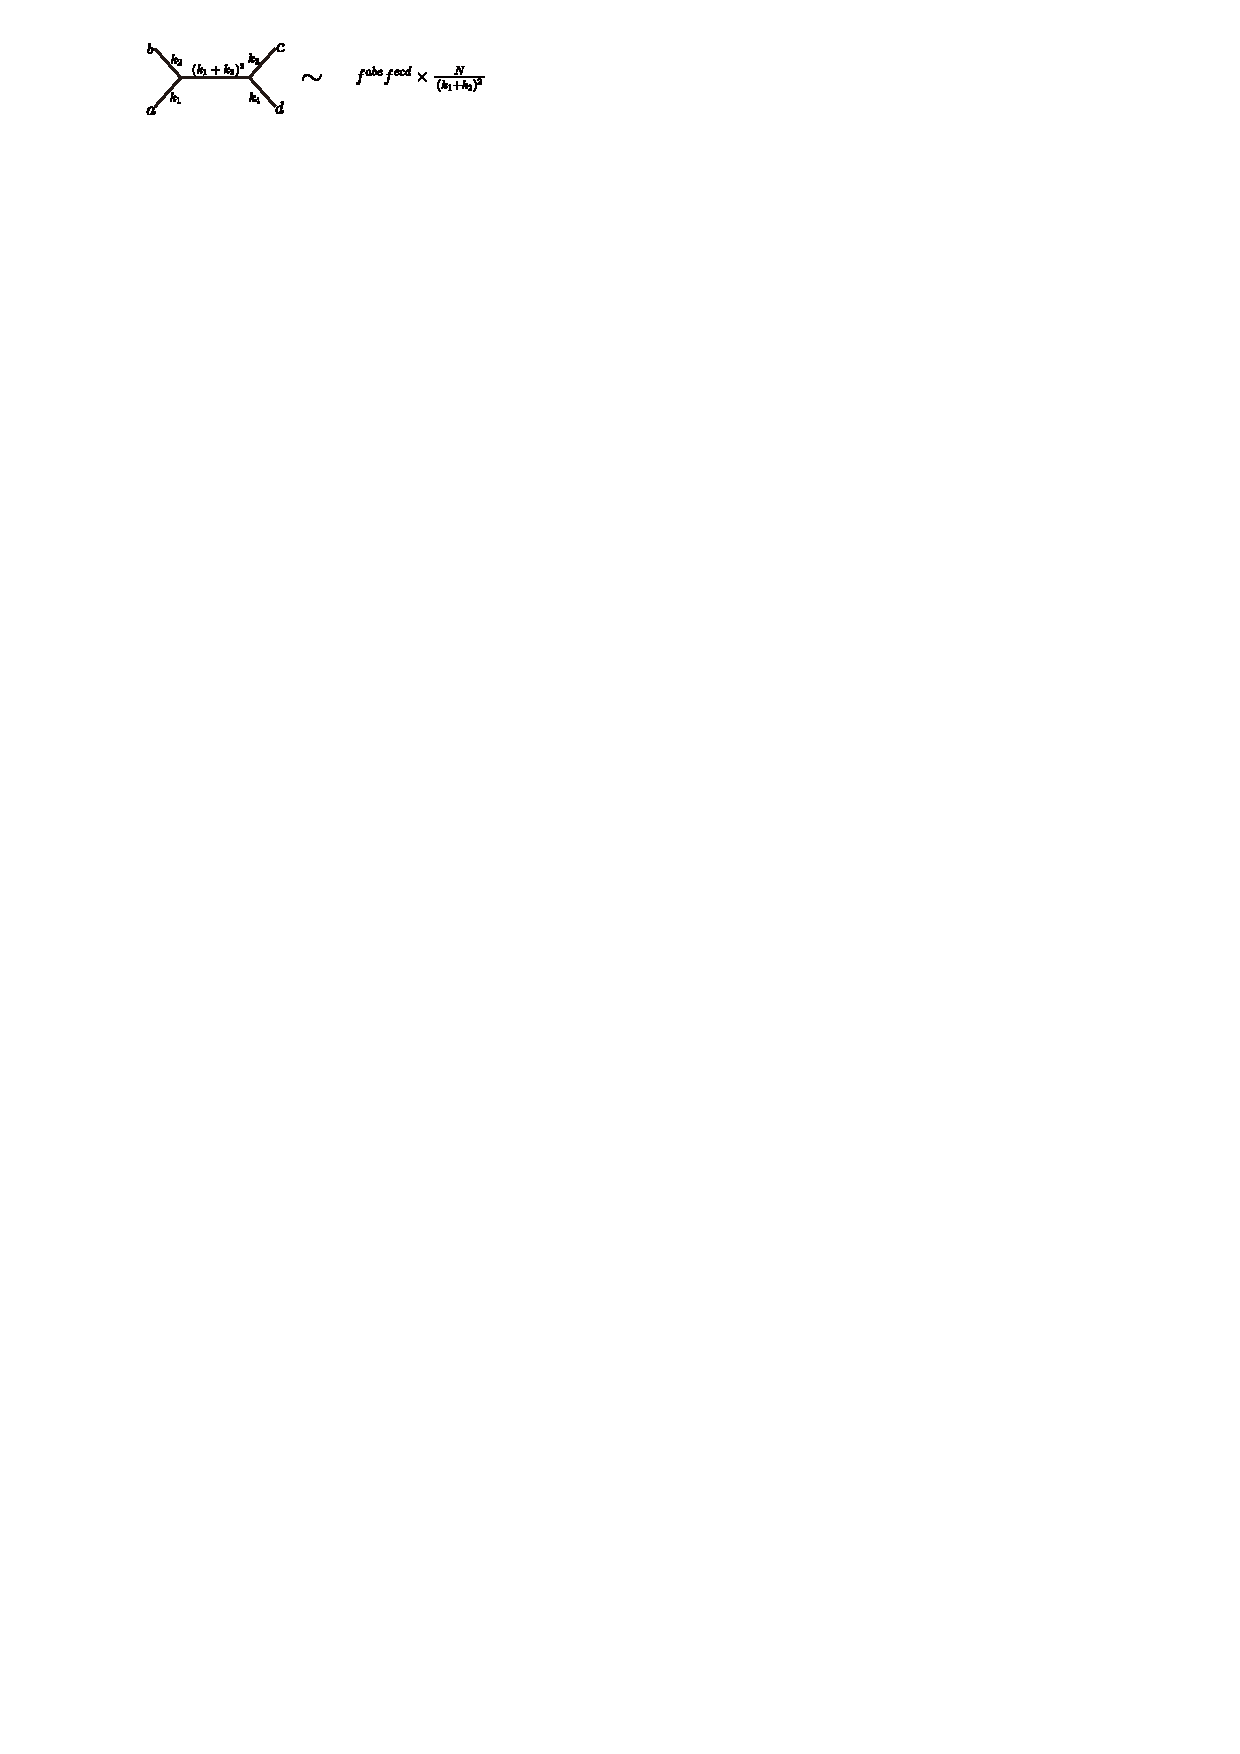
\includegraphics[width=0.8\linewidth]{figs/fig8.pdf}
	\caption{三顶点图“费曼”规则}
	\label{fig:6.1}
\end{figure}

众所周知,Yang-Mills理论费曼规则中不只有三顶角,还有四顶角,乍看之下似乎\ref{eq:6.1}有很大的漏洞。但实际上$\Gamma_n$不应该理解为费曼图,而只是组合学上对振幅的一种编码。但是这种编码的存在性又可以从费曼图本身看出来,比如费曼图四顶角可以用下面的一种方式约化为三顶角:
\begin{equation}
	\parbox[c]{\linewidth}{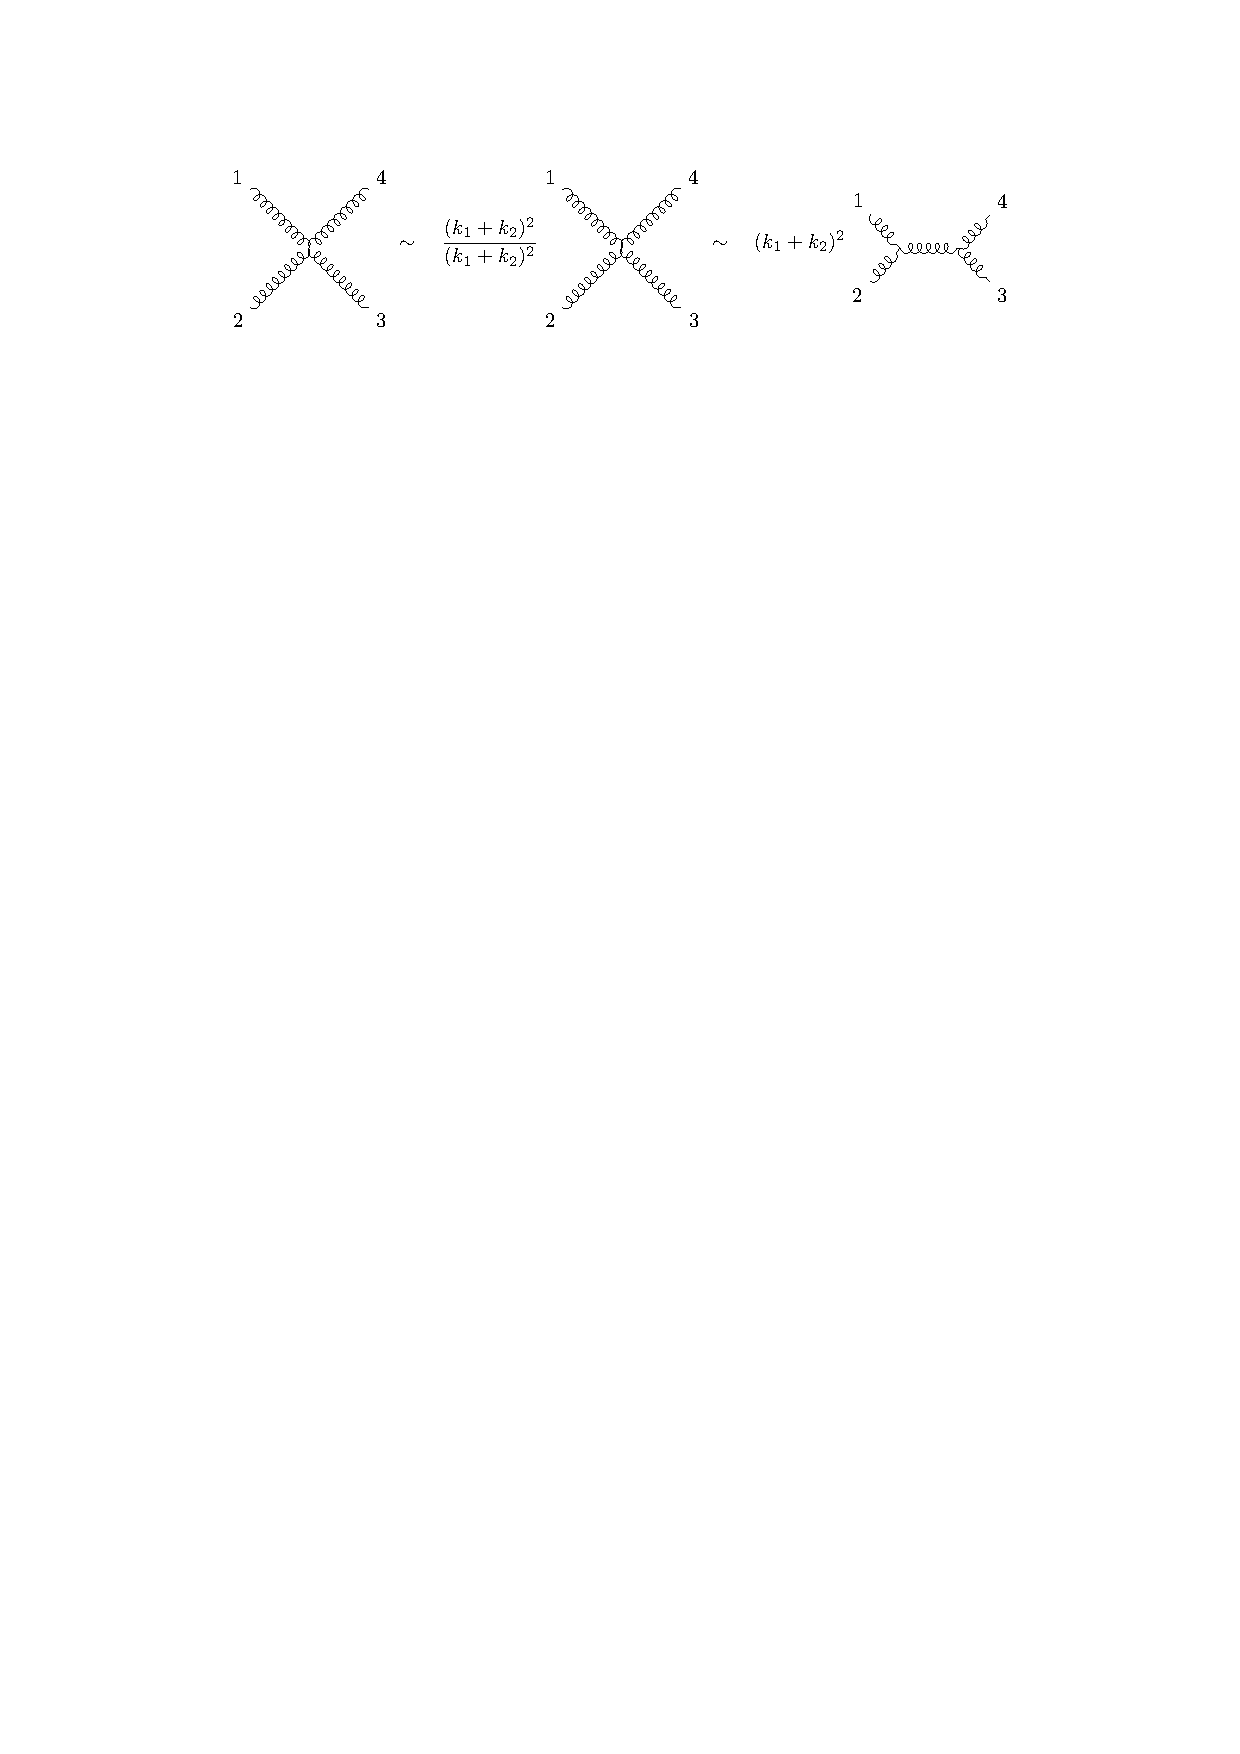
\includegraphics[width=\linewidth]{figs/eq_feyn.pdf}}
\end{equation}
显然,这种编码不是唯一的,但至少存在。结构常数满足如下的Jacobi恒等式:
\begin{equation}
	f^{abe}f^{ecd}+f^{bce}f^{ead}+f^{cae}f^{ebd}=0
\end{equation}
\begin{figure}[htbp]
	\centering
	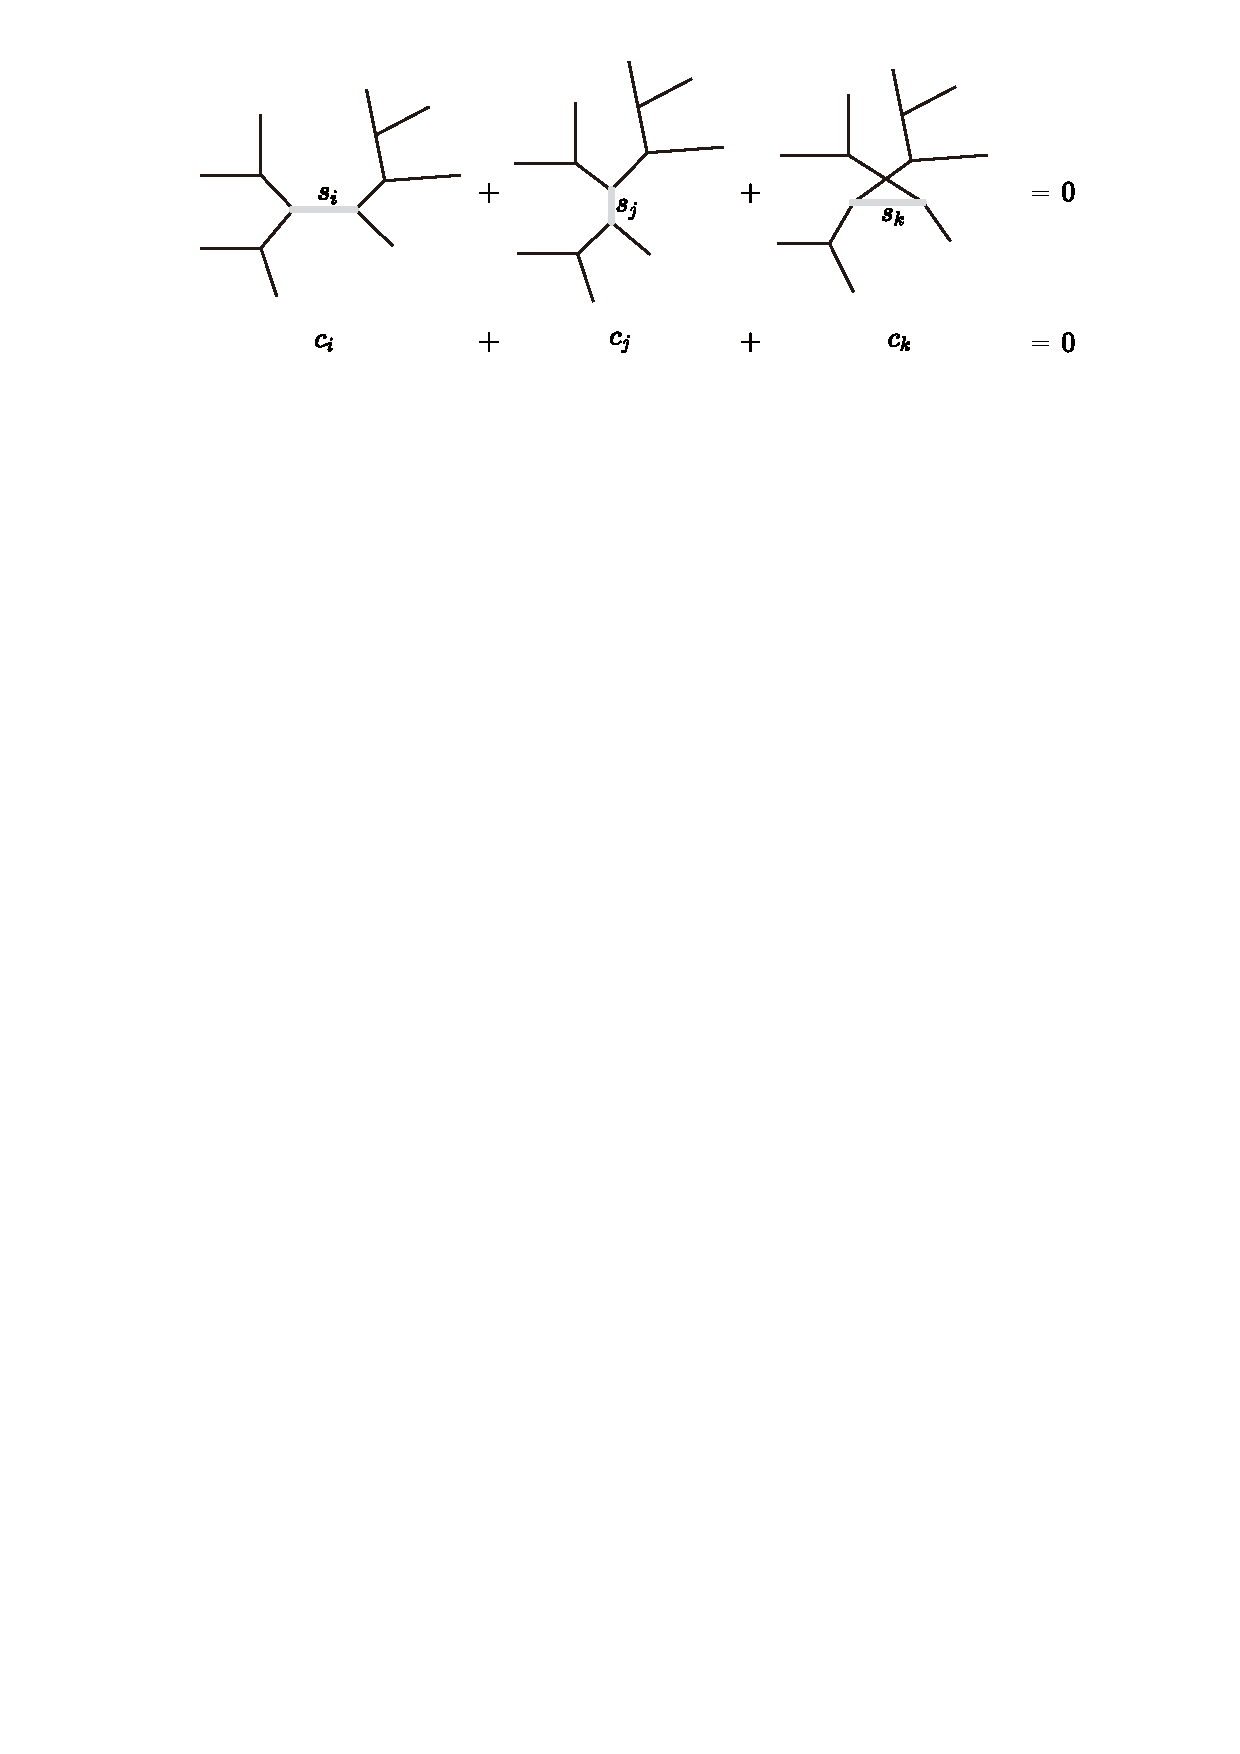
\includegraphics[width=0.95\linewidth]{figs/fig9.pdf}
	\caption{Jacobi恒等式}
	\label{fig:6.2}
\end{figure}
如图\ref{fig:6.2},这意味着三类图的色因子$c$之间的关系。同理$f^{abc}=-f^{acb}$也给出图上的关系。Bern-Carrasco-Johanson猜想存在$\{N_i\}$满足\ref{eq:6.1}而且满足和$\{c_i\}$同样的李代数结构\cite{Bern:2008qj}。也就是说对于任意$i,j,k\in\Gamma_n$:
\begin{equation}
\begin{aligned}
		c_i=-c_j\quad&\Leftrightarrow\quad N_i=-N_j\\
	c_i+c_j+c_k=0\quad&\Leftrightarrow\quad N_i+N_j+N_k=0
\end{aligned}
\end{equation}
这样的$\{N_i\}$称为BCJ分子,这个猜想也被称为色-运动学对偶。而且不难发现BCJ分子的选取不是唯一的,我们总是可以选取任意一个函数$\Delta$做如下变换得到新的BCJ分子:
\begin{equation}
	\label{eq:6.5}
	N_i\to N_i+s_i\Delta,\quad N_j\to N_j+s_j\Delta,\quad N_k\to N_k+s_k\Delta
\end{equation}
这里$s_i$,$s_j$和$s_k$是三幅图各自特有的传播子极点。对于后面要讨论的树图选取$[\lambda^a,\lambda^b] = f^{abc}\lambda^c$以及$\tr [\lambda^a,\lambda^b]=\delta^{ab}$的归一化约定,色基和迹基有如下关系:
\begin{equation}
	\label{eq:6.6}
	f^{a_1a_2x_1}f^{x_1a_3x_2}\cdots f^{x_{n-3}a_{n-1}a_n}=\operatorname{tr}\left(\lambda^{a_1}\left[\lambda^{a_2},[\lambda^{a_3},\ldots,[\lambda^{a_{n-1}},\lambda^{a_n}]\ldots]\right]\right)
\end{equation}
显然$\ref{eq:6.1}$给出如下的色序振幅:
\begin{equation}
	A_n(P)=\sum_{i\in\Gamma_n}\frac{N_i}{D_i}c_i\mid_{\tr (\lambda^P)}
\end{equation}
其中$c_i\mid_{\tr (\lambda^P)}\in\{0,\pm1\}$表示$c_i$中$\tr (\lambda^P)$前的符号。在后面对树图的讨论中,Del Duca–Dixon–Maltoni 基底是十分有用的\footnote{DelDuca:1999rs}:
\begin{equation}
	\label{eq:6.9}
	\mathcal{A}_n = \sum_{\sigma \in S_{n-2}} f^{a_1 a_{\sigma_1} b_1} f^{b_1 a_{\sigma_2} b_2} \cdots f^{b_{n-3} a_{\sigma_{n-2}} a_n} A_n(1, \sigma_1, \sigma_2, \ldots, \sigma_{n-2}, n)
\end{equation}
原本色运动学分离给出迹基底下的展开:
\begin{equation}
	\label{eq:6.10}
	\mathcal{A}_n=\sum_{\sigma\in S_{n-1}}\tr (\lambda^{a_{\sigma_1}}\lambda^{a_{\sigma_2}}\cdots \lambda^{a_{\sigma_{n-1}}}\lambda^{a_n})A_n(\sigma_1,\sigma_2,\ldots,\sigma_{n-1},n)
\end{equation}
但这些色序振幅之间仍有K-K关系\ref{KK},另外色基和迹基之间有关系\ref{eq:6.6},联合起来便可以从\ref{eq:6.10}转换到\ref{eq:6.9}。DDM基底的那些色因子之间是雅可比恒等式意义下独立的,他们对应半梯子图\ref{fig:6.3},后面记其色因子为$c_{1|\sigma|n}$。由于Jacobi恒等式,总可以将\ref{eq:6.1}利用图\ref{fig:6.4}的过程转换成\ref{eq:6.9}的形式。也就是说半梯子图是$\Gamma_n$中的一组独立基底,在构造BCJ分子是我们并不需要半梯子图的$\{N_i\}$之间满足Jacobi恒等式,利用半梯子图用Jacobi恒等式构造剩下的BCJ分子,然后要求求和后刚好得到规范理论振幅。
\begin{figure}[htbp]
	\centering
	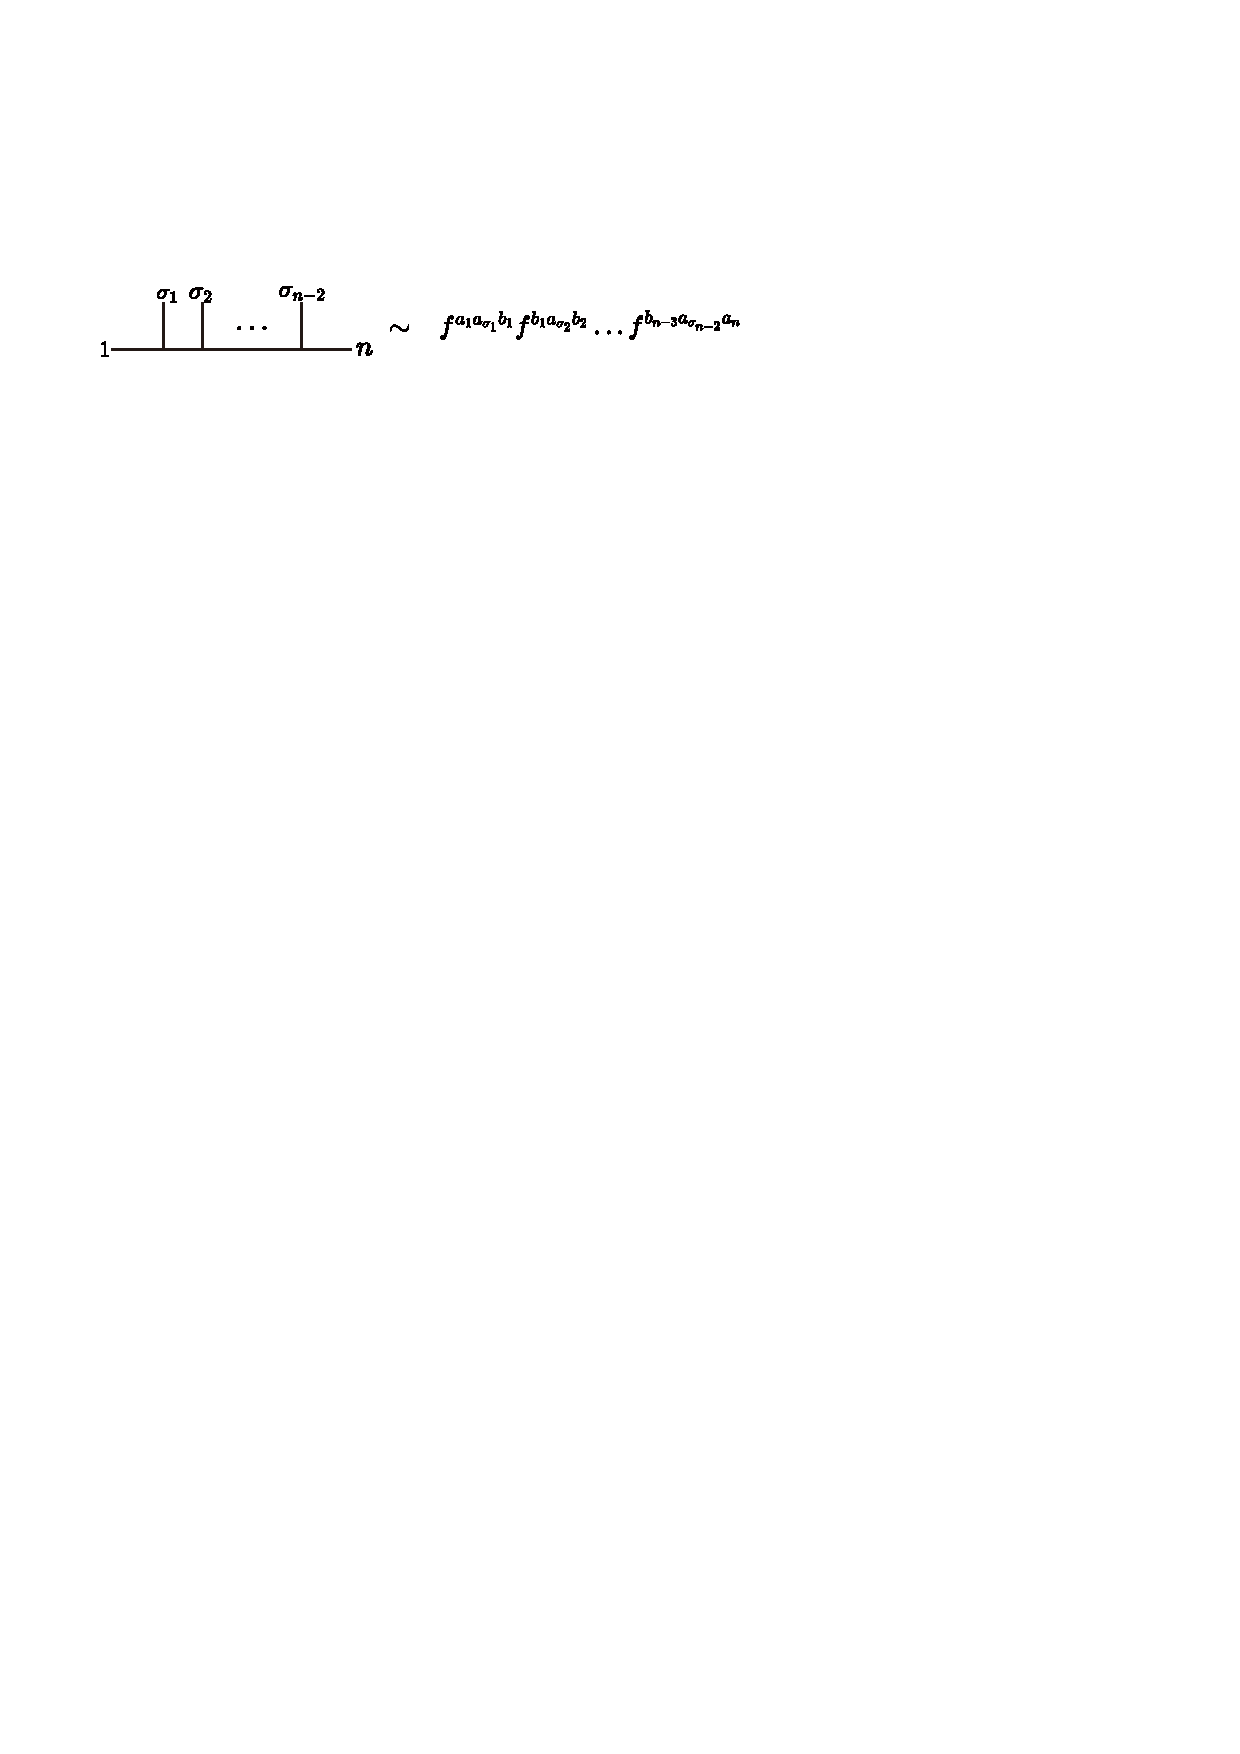
\includegraphics[width=0.95\linewidth]{figs/fig10.pdf}
	\caption{半梯子图}
	\label{fig:6.3}
\end{figure}

\begin{figure}[htbp]
	\centering
	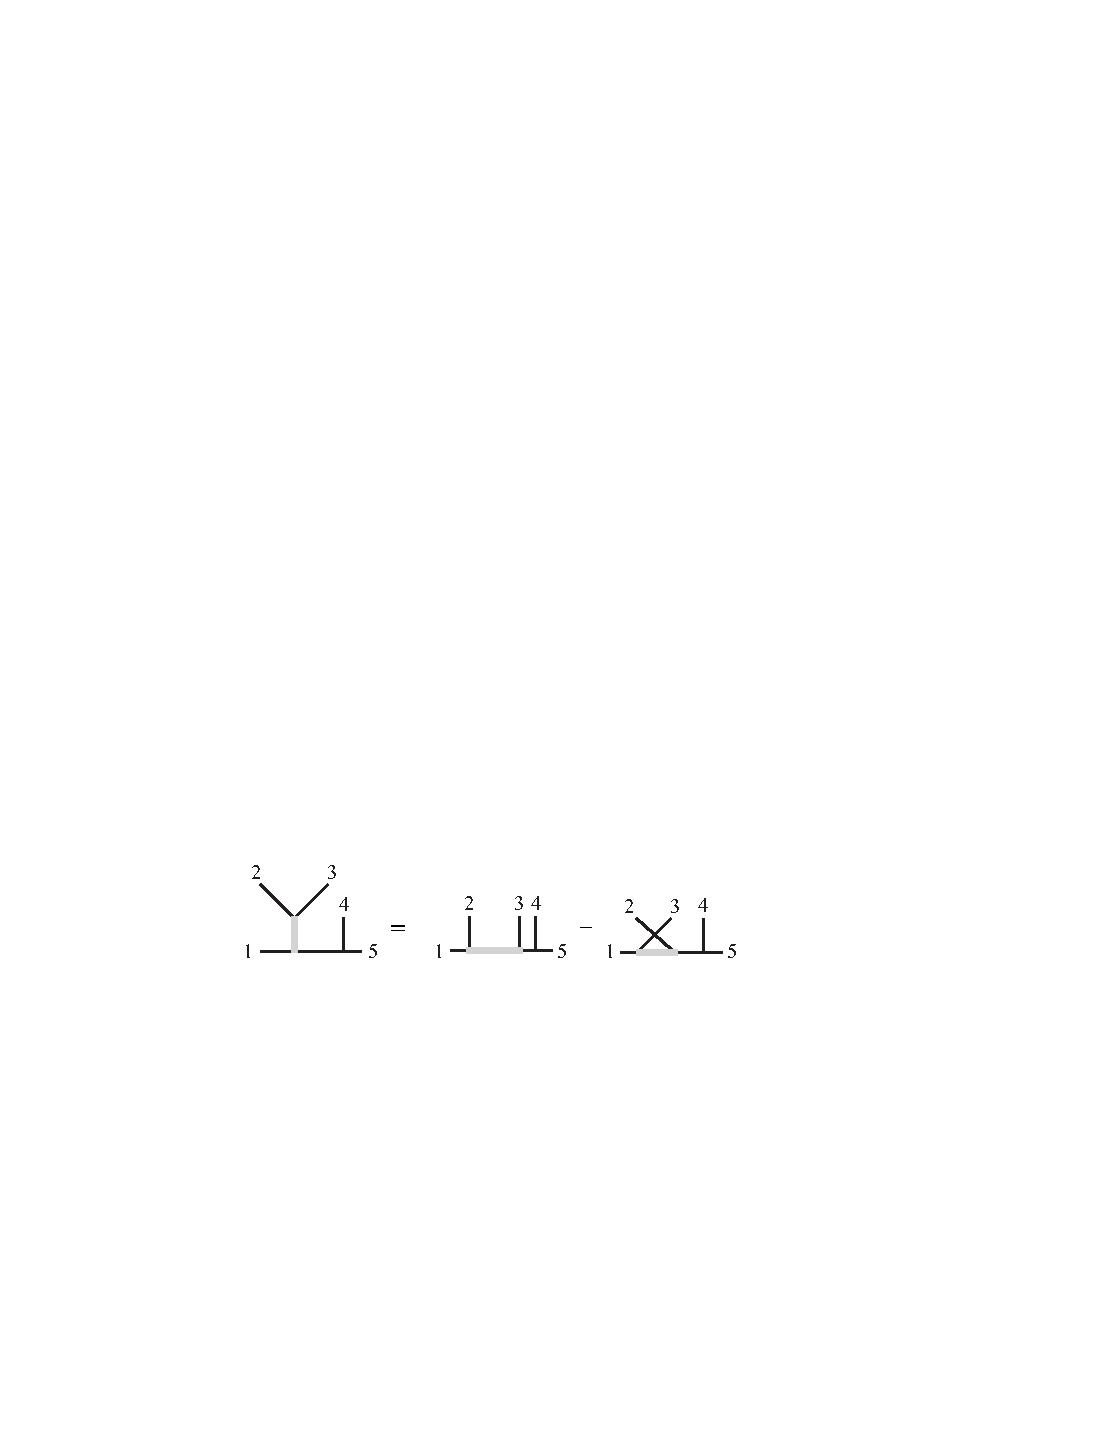
\includegraphics[width=0.90\linewidth]{figs/fig11.pdf}
	\caption{利用Jacobi恒等式转换到半梯子图}
	\label{fig:6.4}
\end{figure}

\begin{figure}[htbp]
	\centering
	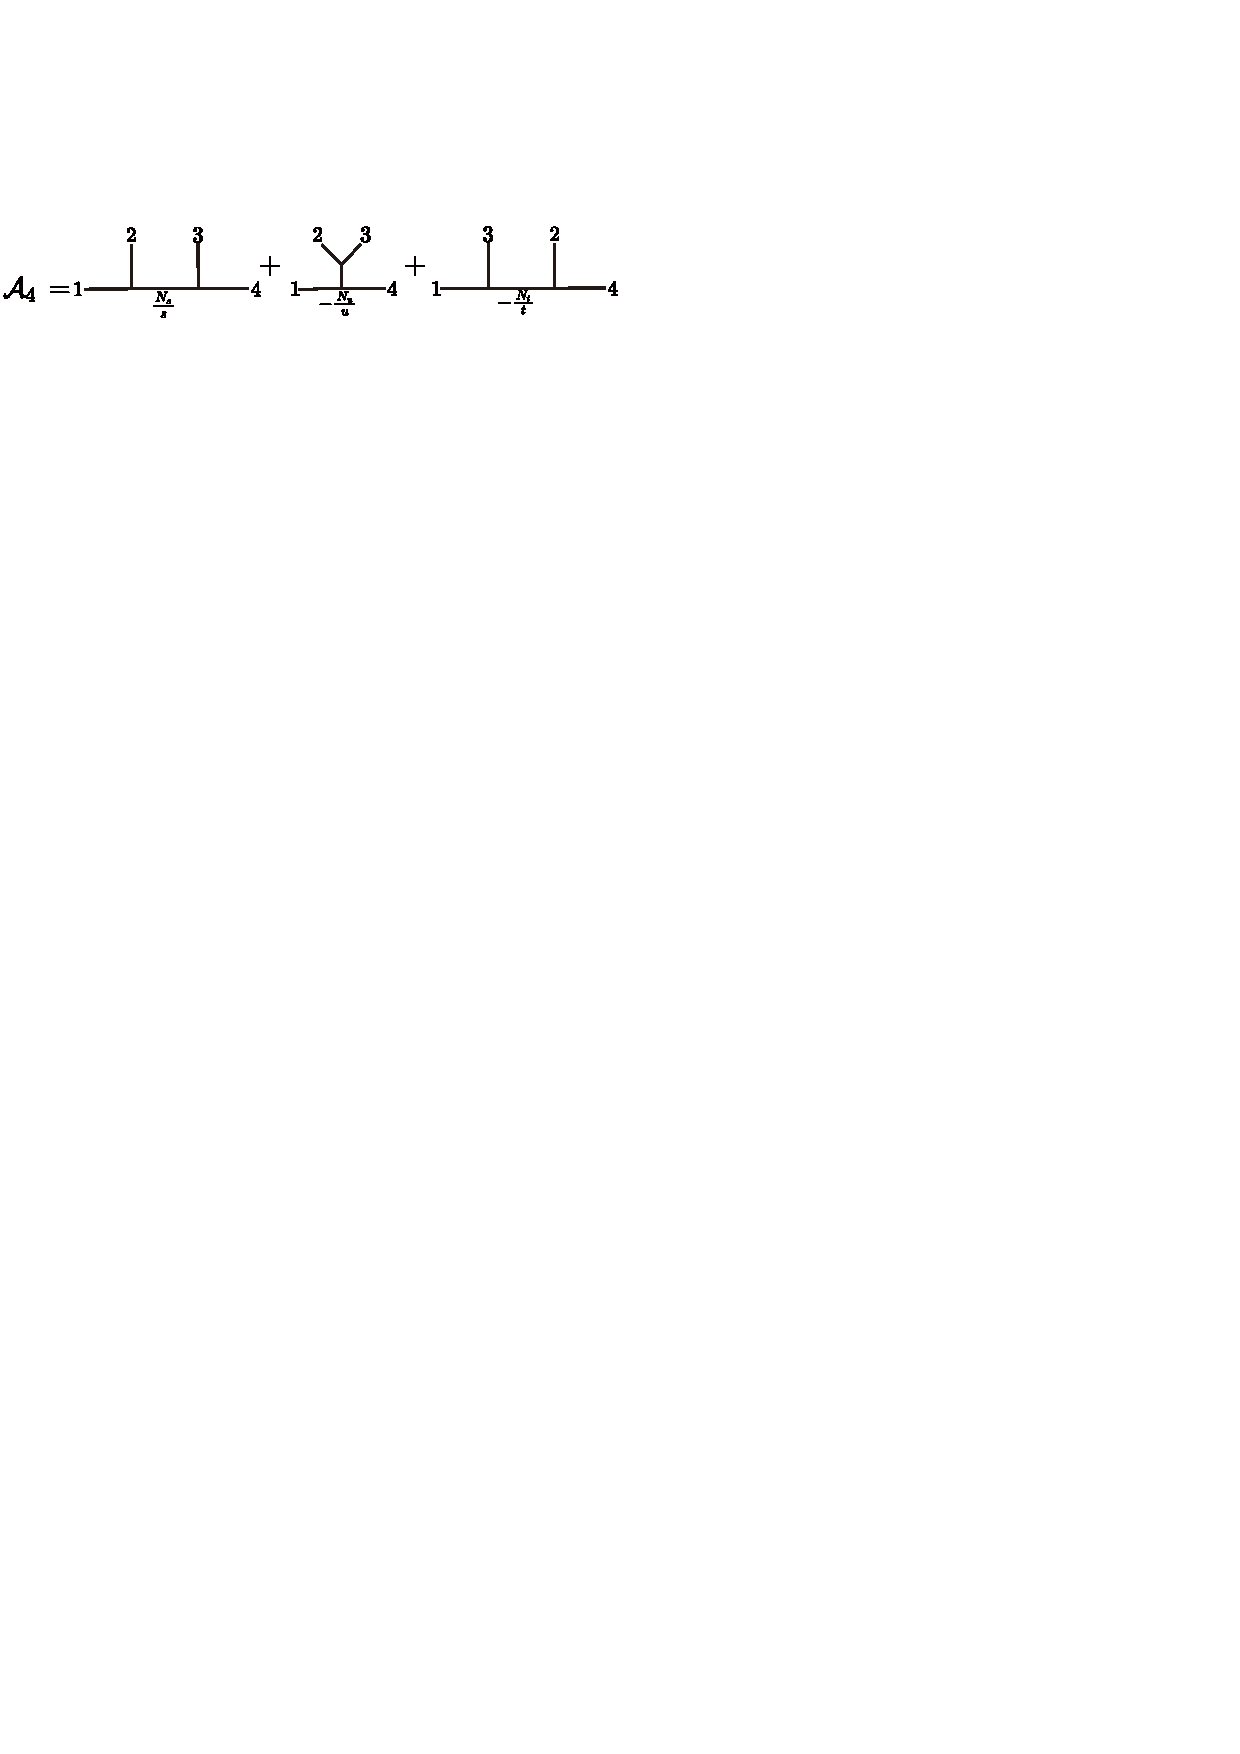
\includegraphics[width=0.90\linewidth]{figs/fig12.pdf}
	\caption{$\Gamma_4$的三幅图}
	\label{fig:6.5}
\end{figure}
比如四点Yang-Mills理论振幅有\ref{fig:6.5}三幅三顶角图有贡献。这里选取正负号约定是为了让$N_s+N_u+N_t=0$,对于树图$m$点情况$|\Gamma_m|=(2m-5)!!$。四点情况下只有两个偏振幅在Jacobi等式的意义下线性独立\footnote{当然如果加入BCJ恒等式两者也线性相关。},选取固定$1$和$4$。将\ref{fig:6.5}中第二个图利用Jacobi恒等式展开到半梯子图得到:
\begin{equation}
	A(1234) = \frac{N_s}{s}-\frac{N_u}{u},\quad A_4(1324)=-\frac{N_t}{t}+\frac{N_u}{u}
\end{equation}
不难看出上面偏振幅在\ref{eq:6.5}的变换下是规范不变的,其实就是在说单个三顶角图不是可观测量,但组合在一起得到的偏振幅规范不变。而且从$N_s+N_t+N_u=0$导出他们满足BCJ恒等式$sA_4(1,2,3,4)=tA_4(1,3,2,4)$。注意,如果$\{N_i\}$是BCJ分子,那么BCJ恒等式自然被满足,但BCJ恒等式本身是和\ref{eq:6.1}的参数化选取无关的,也就是说不管$\{N_i\}$如何选取,最终的振幅之间都满足BCJ恒等式。选取$N_s$和$N_u$为独立变量:
\begin{equation}
	\begin{pmatrix}A_4(1234)\\A_4(1324)\end{pmatrix}=\begin{pmatrix}\frac{1}{s}&-\frac{1}{u}\\\frac{1}{t}&\frac{1}{u}+\frac{1}{t}\end{pmatrix}\begin{pmatrix}N_s\\N_u\end{pmatrix}
\end{equation}
但是由于偏振幅之间满足BCJ恒等式,他们之间不是线性无关的,所以上面的矩阵其实不可逆。而这又恰恰说明了BCJ分子的不唯一性。

上面说的这些都仅仅只是色-运动学之间代数结构上的对偶,而这种对偶和规范理论与微扰引力理论振幅之间又密切关系。进一步有猜想,如果找到了一组BCJ分子,那么引力振幅可以直接由\ref{eq:6.1}得到:
\begin{equation}
	\mathcal{M}_n=\sum_{i\in\Gamma_n}\frac{N_iN_i}{D_i}=\sum_{i\in\Gamma_n}\frac{N_i\tilde{N}_i}{D_i}
\end{equation}
此式称为BCJ双复制关系。第二个等号是说明双复制的$n_i$可以只有一个是BCJ分子,另外一个可以不满足色运动学对偶,但是最终得到的振幅依然相同。利用半梯子图基底可以写成下式:
\begin{equation}
	\label{eq:6.14}
	M_n=\sum_{\sigma\in S_{n-2}}n_{1|\sigma_1,\sigma_2,\ldots,\sigma_{n-2}|n}A_n(1,\sigma_1,\sigma_2,\ldots,\sigma_{n-2},n)
\end{equation}
所以只需要知道半梯子图的BCJ分子就够了。前面我们讲过KLT关系,也是双复制的形式。实际上KLT关系可以看作是树图的一组特殊的BCJ双复制关系,可以从KLT关系直接构造出半梯子图的BCJ分子从而用Jacobi恒等式得到三顶点图的全部BCJ分子,比如四点五点KLT关系为:
\begin{equation}
\begin{aligned}
	M_4(1234)&=-s_{12}A_4(1234)A_4(1243),\\M_5(12345)&=s_{23}s_{45}A_5(12345)A_5(13254)+(3\leftrightarrow4)
\end{aligned}
\end{equation}
与\ref{eq:6.14}对照可以得到BCJ分子:
\begin{equation}
	\begin{aligned}
		n=4:\quad & n_{12,34} = -s_{12}\,A^{\text{tree}}_{4}[1243], \quad n_{13,24} = 0; \\
		n=5:\quad & n_{12,3,45} = s_{23}\,s_{45}\,A^{\text{tree}}_{5}[13254], \quad n_{12,4,35} = s_{24}\,s_{35}\,A^{\text{tree}}_{5}[14253]; \\
		& n_{13,4,25} = n_{14,2,35} = n_{14,3,215} = n_{12,3,415} = 0.
	\end{aligned}
\end{equation}
树图的BCJ双复制关系已经得到证明\cite{Bern:2010yg},但目前对于圈图BCJ分子的构造仍是一个未解之谜,不过已经构造出了不少例子\cite{Bern:2010ue,Bern:2012uf},这也让我们相信色-运动学对偶猜想的正确性。近年来,双复制关系也被用在引力波求解等问题上,详见综述\cite{Bern:2019prr,Adamo:2022dcm,Bern:2022wqg}。

\section{纯旋量超弦关联函数计算}
纯旋量形式计算涉及到OPE计算以及展开超场后计算鬼场零模,本章我们不去关注后面一部分,而关注如何计算OPE。从$\S$\ref{sec:5.4}可以看出如果直接使用$\partial\theta$,$\Pi$,$d$,$N$的OPE计算会非常复杂,我们试图把顶角算符本身作为一个整体来计算OPE,比如:
\begin{equation}
	V_1(z_1)V_2(z_2)\sim 0
\end{equation}
\begin{equation}
	\label{eq:6.17}
	V_1(z_1)U_2(z_2)\sim z_{12}^{-k_1\cdot k_2}\frac{L_{12}(z_2)}{z_{12}},\quad L_{12}:=-A_2^m(\lambda\gamma_mW_1)-V_2(k_2\cdot A_1)+Q(A_2W_1)
\end{equation}
\begin{equation}
	\label{eq:6.18}
	\begin{aligned}
		U_1(z_1)U_2&(z_2)\sim z_{12}^{-k_1\cdot k_2-1}\left(\partial\theta^\alpha\Big[(k_1\cdot A_2)A_\alpha^1-(k_2\cdot A_1)A_\alpha^2+D_\alpha A_\beta^2W_1^\beta-D_\alpha A_\beta^1W_2^\beta\Big]\right.\\&+\Pi^m\Big[(k_1\cdot A_2)A_m^1-(k_2\cdot A_1)A_m^2+k_m^2(A_2W_1)-k_m^1(A_1W_2)-(W_1\gamma_mW_2)\\&+d_\alpha\left[(k_1\cdot A_2)W_1^\alpha-(k_2\cdot A_1)W_2^\alpha+\frac14(\gamma^{mn}W_1)^\alpha F_{mn}^2-\frac14(\gamma^{mn}W_2)^\alpha F_{mn}^1\right]\\&+\frac12N^{mn}\Big[(k_1\cdot A_2)F_{mn}^1-(k_2\cdot A_1)F_{mn}^2-2k_m^{12}(W_1\gamma_nW_2)+2F_{ma}^1F_{na}^2\Big]\Big)\\&+(1+k_1\cdot k_2)z_{12}^{-k_1\cdot k_2-2}\left[(A_1W_2)+(A_2W_1)-(A_1\cdot A_2)\right]
	\end{aligned}
\end{equation}
其中$Q$是BRST荷,利用$d_\alpha$和超场的OPE,后面的计算可以将$Q$看作是$\lambda^\alpha D_\alpha$。计算中涉及到对超场求导,而平面波求导会出现$ik$因子,为了避免频繁出现虚数单位,我们选取约定$ik\to k$,从而Mandelstam变量与惯用的也相差$-1$。另外,我们隐藏$A^\mu$和$A_\alpha$指标,用$\cdot$表示矢量指标求和,旋量指标求和则不加任何标记。而且假设所有的超场都是$K(\theta)$,已经分离平面波。乍看之下似乎看不出规律,但倘若定义:
\begin{equation}
	\label{eq:6.19}
	\begin{aligned}
		&A_\alpha^{12}=\frac{1}{2}\left[A_\alpha^2(k_2\cdot A_1)+A_2^m(\gamma_mW_1)_\alpha-(1\leftrightarrow2)\right]
		\\&A_{12}^m=\frac{1}{2}\left[A_2^m(k_2\cdot A_1)+A_p^1F_2^{pm}+(W_1\gamma^mW_2)-(1\leftrightarrow2)\right]
		\\&W_{12}^{\alpha}=\frac{1}{4}(\gamma_{mn}W_2)^\alpha F_1^{mn}+W_2^\alpha(k_2\cdot A_1)-(1\leftrightarrow2)
		\\&F_{12}^{mn}=F_2^{mn}(k_2\cdot A_1)+\frac{1}{2}F_2^{[m}F_1^{n]p}+k_1^{[m}(W_1\gamma^{n]}W_2)-(1\leftrightarrow2)
	\end{aligned}
\end{equation}
\ref{eq:6.18}变成:
\begin{equation}
	\label{eq:6.20}
	\begin{aligned}
		&U_1(z_1)U_2(z_2)\sim-z_{12}^{-k_1\cdot k_2-1}\left(\partial\theta^\alpha A_\alpha^{12}+\Pi^mA_m^{12}+d_\alpha W_{12}^\alpha+\frac{1}{2}N^{mn}F_{mn}^{12}\right)\\&+\partial_1\left(z_{12}^{-k_1\cdot k_2-1}\left[\frac{1}{2}(A_1\cdot A_2)-(A_1W_2)\right]\right)-\partial_2\left(z_{12}^{-k_1\cdot k_2-1}\left[\frac{1}{2}(A_1\cdot A_2)-(A_2W_1)\right]\right)
	\end{aligned}
\end{equation}
注意到$U$是积分顶角算符,可以预料到这些全导数项应当能够忽略,得到下面的等效OPE:\footnote{\ref{eq:6.20}中的$z_{12}^{-k_1\cdot k_2}$因子来源于平面波给出的Koba-Nielsen因子,注意这里我们已经假设所有的超场都是不带平面波因子的,这从运动方程就能看出来这一约定。最后计算振幅只需要补上Koba-Nielsen因子即可。}\footnote{似乎在OPE之后还会剩下$\partial\theta,\Pi,\ldots$,并非超场零模积分,但注意到盘面振幅始终存在无积分顶角算符插入,所以最终振幅一定可以用$\langle V_P\rangle$表示。}
\begin{equation}
	U_1(z_1)U_2(z_2)\cong \frac{U_{12}(z_2)}{z_{12}}, \quad U_{12}:=\partial\theta^\alpha A_\alpha^{12}+\Pi^mA_m^{12}+d_\alpha W_{12}^\alpha+\frac{1}{2}N^{mn}F_{mn}^{12}
\end{equation}
同理,注意到下式BRST恰当:
\begin{equation}
	L_{21}+L_{12}=Q\left[(A_1W_2)+(A_2W_1)-(A_1\cdot A_2)\right]
\end{equation}
所以$L_{12}$的对称部分应当和体系解耦,利用\ref{eq:6.17}以及\ref{eq:6.19}不难验算在去除掉所有BRST恰当的项之后有如下等效OPE:
\begin{equation}
	V_1(z_1)U_2(z_2)\cong \frac{V_{12}(z_2)}{z_{12}},\quad
	V_{12} := \lambda^\alpha A_\alpha^{12}
\end{equation}
代入\ref{eq:5.45}得到新定义的包含多个指标的超场(多粒子超场)满足:
\begin{equation}
	\begin{aligned}
		D_\alpha A_\beta^{12}+D_\beta A_\alpha^{12}&=\gamma_{\alpha\beta}^mA_m^{12}{\color{blue}+(k_1\cdot k_2)(A_\alpha^1A_\beta^2+A_\beta^1A_\alpha^2)}
		\\D_\alpha A_{12}^m&=\gamma_{\alpha\beta}^mW_{12}^\beta{+\color{blue}k_{12}^mA_\alpha^{12}+(k_1\cdot k_2)(A_\alpha^1A_2^m-A_\alpha^2A_1^m)}
		\\D_\alpha W_{12}^\beta&=\frac{1}{4}(\gamma_{mn})_\alpha^\beta F_{12}^{mn}{\color{blue}+(k_1\cdot k_2)(A_\alpha^1W_2^\beta-A_\alpha^2W_1^\beta)}
		\\D_\alpha F_{12}^{mn}&=k_{12}^{[m}(\gamma^{n]}W_{12})_\alpha{\color{blue}+(k_1\cdot k_2)\left[A_\alpha^1F_2^{mn}+A_1^{[n}(\gamma^{m]})W_2)_\alpha-(1\leftrightarrow2)\right]}
	\end{aligned}
\end{equation}
\begin{equation}
	F_{12}^{mn}=k_{12}^mA_{12}^n-k_{12}^nA_{12}^m{\color{blue}-(k_1\cdot k_2)(A_1^mA_2^n-A_1^nA_2^m)}
\end{equation}
不难发现相比于\ref{eq:5.45}多了蓝色标出的“接触项”,同样的,多粒子顶角算符也会多出一些接触项,而不是简单的BRST闭:
\begin{equation}
	\label{eq:6.26}
	\begin{aligned}
		QV_{12}&={\color{blue}(k_1\cdot k_2)V_1V_2}\\
		QU_{12}&=\partial V_{12}{\color{blue}+(k_1\cdot k_2)(V_1U_2-V_2U_1)}
	\end{aligned}
\end{equation}
但倘若我们能找到接触项的一般表达式,解相应的场方程找到多粒子超场类似单粒子超场的$\theta$展开,那么我们就能利用OPE的规律很快解决振幅计算问题。Mafra和Schlotterer正是利用这一点得到了超弦无质量态$n$点盘面振幅的一般公式\cite{Mafra:2011nv,Mafra:2011nw},接下来我们先来研究一般的多粒子超场。
\subsection{多粒子超场}
前面两个顶角算符的缩并我们改为使用$V_{[1,2]}$表示,不难发现$V_{12} = -V_{21}$确实有李括号带来的反对易性。类似的,还会有多个缩并,比如$U_1(z_1)U_2(z_2)U_3(z_3)$:
\begin{equation}
	U_{[[1,2],3]}(z_3),\quad U_{[1,[2,3]]}(z_3),\quad U_{[1,[2,3]]}(z_3)
\end{equation}
这种下标称为李多项式\footnote{之后大写字母$P,Q,\ldots$表示李多项式或者字词,从上下文不至于混淆。},数学方面的介绍可见\cite{REUTENAUER2003887, free_lie,lothaire1997combinatorics},更偏向物理的介绍可见\cite{Frost:2020eoa}。使用这种下标的好处是显现出了最终我们得到的多粒子超场/顶角算符关于指标的对称性,后面我们会尽可能构造超场使得其拥有李多项式所满足的对称性,这是本文后面用于构建BCJ分子的核心。现在我们期望多个顶角算符缩并得到的$U_\Gamma$和$V_{\Gamma}$仍像上一节一样可以通过定义对应的$A^\Gamma$,$W^\Gamma$和$F^\Gamma$得到类似顶角算符的形式。后面定义多粒子超场都是在李多项式的意义下定义的,对下指标做线性扩张便可得到对字词定义的多粒子超场。比如$V_{12}$\footnote{不要与上一小节中的$V_{12}$弄混。}就是$V_{[1,2]}$的对称部分。

由于多粒子超场本身来源于单粒子超场,而单粒子超场本身是离壳的,也就是说存在规范对称性。比如展开单粒子超场时就使用的是Harnad–Shnider规范。所以多粒子场本身也应当有这种规范选取带来的不唯一性,下面逐一讨论。
\subsubsection{Lorenz规范}
最早在Lorenz规范$\partial\cdot A^P = 0 $下找到了多粒子超场满足的递推公式:
\begin{equation}
	\begin{aligned}
	\hat{A}_\alpha^{[P,Q]}&=\frac{1}{2}\left[\hat{A}_\alpha^Q(k_Q\cdot\hat{A}_P)+\hat{A}Q^m(\gamma_m\hat{W}_P)\alpha-(P\leftrightarrow Q)\right]\\
	\hat{A}_{[P,Q]}^m&=\frac{1}{2}\left[\hat{A}_Q^m(k_Q\cdot\hat{A}_P)+\hat{A}_n^P\hat{F}_Q^{nm}+(\hat{W}_P\gamma^m\hat{W}_Q)-(P\leftrightarrow Q)\right]\\
	\hat{W}_{[P,Q]}^{\alpha}&=\frac{1}{4}\hat{F}_P^{rs}(\gamma_{rs}\hat{W}_Q)^\alpha+\frac{1}{2}(k_Q\cdot\hat{A}_P)\hat{W}_Q^\alpha+\frac{1}{2}\hat{W}_Q^{m\alpha}\hat{A}_m^P-(P\leftrightarrow Q)\\
	\hat{F}_{[P,Q]}^{mn}&=\frac{1}{2}{\left[\hat{F}_Q^{mn}(k_Q\cdot\hat{A}_P)+\hat{F}_Q^{p|mn}\hat{A}_p^p+\hat{F}_Q^{[m}\hat{F}_P^{n]r}-2\gamma_{\alpha\beta}^{[m}\hat{W}_P^{n]\alpha}\hat{W}_Q^\beta-(P\leftrightarrow Q)\right]}
\end{aligned}
\end{equation}
递推初始项来源于$\hat K_i = K_i$,动量应当理解为无视李括号,比如$k_{[1,[2,3]]}:=k_{123}:=\sum_{i=1}^3k_i$。其中:
\begin{equation}
\begin{aligned}
		\hat{W}_{[P,Q]}^{m\alpha} &= k_{PQ}^m \hat{W}_{[P,Q]}^\alpha - (\hat{A}^m \otimes \hat{W}^\alpha)_{C([P,Q])} \\
	\hat{F}_{[P,Q]}^{m|pq} &= k_{PQ}^m \hat{F}_{[P,Q]}^{pq} - (\hat{A}^m \otimes \hat{F}^{pq})_{C([P,Q])}
\end{aligned}
\end{equation}
这里我们引入了接触项算符$C$,递归定义为,$C(i):= 0 $:
\begin{equation}
	C([P,Q]):=[C(P),Q]+[P,C(Q)]+(k_P\cdot k_Q)(P\otimes Q-Q\otimes P)
\end{equation}
张量积满足莱布尼茨律:
\begin{equation}
\begin{aligned}
		[A\otimes B,Q]:=[A,Q]\otimes B+A\otimes[B,Q]\\
	[P,A\otimes B]:=[P,A]\otimes B+A\otimes[P,B]
\end{aligned}
\end{equation}
后面还会用到反对易楔积的定义:
\begin{equation}
	P\wedge Q:=P\otimes Q-Q\otimes P
\end{equation}
且依照线性扩张定义:
\begin{equation}
	(K\otimes T)_{P\otimes Q}:=K_PT_Q,\quad(K\wedge T)_{P\wedge Q}:=K_PT_Q
\end{equation}
把$C$称为接触项算符是有原因的,超场运动方程的接触项恰好是由$C[P,Q]$生成的:
\begin{equation}
\begin{aligned}
	D_{(\alpha}\hat{A}_{\beta)}^{[P,Q]}&=\gamma_{\alpha\beta}^m\hat{A}_m^{[P, {Q}]}{\color{blue}+(\hat{A}_\alpha\otimes\hat{A}_\beta)_{ {C}([P, {Q}])}}
	\\D_\alpha\hat{A}_m^{[P,Q]}&=(\gamma_m\hat{W}^{[P, {Q}]})_\alpha+k_m^{ {PQ}}\hat{A}_\alpha^{[P, {Q}]}{\color{blue}+(\hat{A}_\alpha\otimes\hat{A}^m)_{ {C}([P, {Q}])}}
	\\D_\alpha\hat{W}_{[P, {Q}]}^\beta&=\frac{1}{4}(\gamma^{mn})_\alpha^\beta\hat{F}_{mn}^{[P,Q]}{\color{blue}+(\hat{A}_\alpha\otimes\hat{W}^\beta)_{C([P,Q])}}
	\\D_\alpha\hat{F}_{[P,Q]}&=\left(\hat{W}_{[P,Q]}^{[m}\gamma^{n]}\right)_\alpha{\color{blue}+(\hat{A}_\alpha\otimes\hat{F}^{mn})_{ {C}([P,Q])}}
\end{aligned}
\end{equation}
\begin{equation}
	\label{eq:6.35}
	\hat{F}_{[P,Q]}^{mn}=k_{PQ}^m\hat{A}_{[P,Q]}^n-k_{PQ}^m\hat{A}_{[P,Q]}^m{\color{blue}-(\hat{A}^m\otimes\hat{A}^n)_{C([P,Q])}}
\end{equation}
\subsubsection{混合(hybrid)规范}
Dynkin括号递归定义为:
\begin{equation}
	\ell(123\ldots n):=[\ell(123\ldots n-1),n]
\end{equation}
其满足下面的Baker恒等式:
\begin{equation}
	\ell(P\ell(Q))=[\ell(P),\ell(Q)]
\end{equation}
显然$A\ell(B)+B\ell(A)\in\ker\ell$,而且由$\ell$的递归定义知$\forall Q$,$\ell(P) = 0\Rightarrow \ell(PQ)=0$。前面说过我们希望多粒子超场的定义尽可能展现出李多项式本身的对称性,那么如果$K\approx \ell$,也就是说满足下面的广义BCJ恒等式:
\begin{equation}
	\label{eq:6.38}
	K_{A\ell(B)C}+K_{B\ell(A)C}=0,\quad A,B\neq\varnothing,\quad\forall C
\end{equation}
这样的超场被称作处在BCJ规范的超场,不加任何符号以区分Lorenz等规范下超场。本节要介绍的混合规范本身并不是计算上会用到的规范,更应该看作是为了构造BCJ规范超场的一种定义:
\begin{equation}
	\begin{aligned}
		\check{A}_\alpha^{[P,  {Q}]}&=\frac{1}{2}[A_\alpha^  {Q}(k_Q\cdot A_P)+A_Q^m(\gamma_mW_P)_\alpha-(P\leftrightarrow Q)]
		\\\check{A}_{[P,  {Q}]}^m&=\frac{1}{2}[A_Q^m(k_Q\cdot A_P)+A_n^PF_Q^{nm}+(W_P\gamma^mW_Q)-(P\leftrightarrow Q)]\\
		\check{W}_{[P,  {Q}]}^\alpha&=\frac{1}{4}F_P^{rs}(\gamma_{rs}W_Q)^\alpha+\frac{1}{2}(k_Q\cdot A_P)W_Q^\alpha+\frac{1}{2}W_Q^{m\alpha}A_P^m-(P\leftrightarrow Q)\\
		\check{F}_{[P,  {Q}]}^m&=\frac{1}{2}{\left[F_Q^{mn}(k_Q\cdot A_P)+F_Q^{r|mn}A_r^P+F_Q^{[m}{}_rF_P^{n]r}-2\gamma_{\alpha\beta}^{[m}W_P^{n]\alpha}W_Q^\beta-(P\leftrightarrow Q)\right]}\\
		W_{[P,Q]}^{m\alpha}&:=k_{PQ}^mW_{[P,Q]}^\alpha-(A^m\otimes W^\alpha)_{C([P,Q])}\\
		F_{[P,Q]}^{m|pq}&:=k_{PQ}^mF_{[P,Q]}^{pq}-(A^m\otimes F^{pq})_{C([P,Q])}
	\end{aligned}
\end{equation}
这并非递归的定义,因为等式右边不是$\check K$,而是BCJ规范下的超场。
\subsubsection{BCJ规范}
利用上一小节给出的混合规范,可以构造BCJ规范下的超场:
\begin{equation}
	\begin{aligned}
		K_{[P,Q]}&:=\check{K}_{[P,Q]}-\sum_{\delta(Y)=R\otimes S}(k_X\cdot k_j)\left[H_{[XR,Q]}K_{jS}-(X\leftrightarrow j)\right]\\&+\sum_{\substack{  {Q}=  {X}j  {Y}\\{{\delta(Y)=R\otimes S}}}}(k_X\cdot k_j)\left[H_{[XR,P]}K_{jS}-(X\leftrightarrow j)\right]-\begin{cases}D_\alpha H_{[P,  {Q}]}&:K=A_\alpha\\k_{{  {P}  {Q}}}^mH_{[P,  {Q}]}&:K=A^m\\0&:K=W^\alpha\end{cases}
	\end{aligned}
\end{equation}
其中:
\begin{equation}
	H_{[i,j]}=0,\quad H_{[A,B]}=(-1)^{|B|}\frac{|A|}{|A|+|B|}\sum_{XjY=\dot{a}\tilde{B}}(-1)^{|Y|}H_{\tilde{Y},j,X}^{\prime}-(A\leftrightarrow B)
\end{equation}
\begin{equation}
	\begin{aligned}
		H_{A,B,C}^{\prime}:=&H_{A,B,C}+\left[\frac{1}{2}H_{[A,B]}(k_{AB}\cdot A_C)+\operatorname{cyc}(A,B,C)\right]\\&-\left[\sum_{\substack{XjY=A\\{\delta(Y)=R\otimes S}}}(k_X\cdot k_j)[H_{[XR,B]}H_{[jS,C]}-(X\leftrightarrow j)\right]+\operatorname{cyc}(A,B,C)
		\\H_{A,B,C}:=&-\frac{1}{4}A_A^mA_B^nF_C^{mn}+\frac{1}{2}(W_A\gamma_mW_B)A_C^m+\operatorname{cyc}(A,B,C).\end{aligned}
\end{equation}
然后是一些组合学上的记号,洗牌序$\shuffle$对应的反运算$\delta$定义为:
\begin{equation}
	\delta(P)=\sum_{X,Y}\langle P,X\shuffle Y\rangle X\otimes Y
\end{equation}
其中内积定义为:
\begin{equation}
	\langle{A,B}\rangle:=\delta_{A,B}
\end{equation}
$\tilde B$意思为反序,$\dot a$表示$A$的字符化,比如$12\mapsto (12)$,在后面的计算中$(12)$作为一个整体不能分开,比如$XY=(12)$是无解的,而不像$XY=12$有一个解为$X=1$,$Y=2$。

现在回到最初对两个顶角算符OPE的研究,那里我们将$V_{[1,2]}=V_{\ell(12)}$记为$V_{12}$,这是有原因的。由于BCJ规范下超场的构造在数学上相当于$\ell\leftrightarrow K$,注意到$\ell\circ\ell(P) = |P|\ell (P)$,对应到超场有$K_{\ell(P)} = |P|K_P$仅仅只相差一个常数,而且由于最终的目的是计算OPE缩并,所以我们不会使用到单个单词对应的超场,都是李多项式对应的超场,所以我们干脆取符号约定$K_{\ell(P)} := K_P$,这个意思是把所有超场下标中连续的单词都看作嵌套括号,比如$K_{123}:=K_{\ell(123)}$,$K_{[12,34]}:=K_{[\ell(12),\ell(34)]}$。在这一符号约定下,依然满足广义BCJ恒等式\ref{eq:6.38}。再注意利用Baker恒等式总可以将任意的$K_\Gamma$写成$K_{1P}$的线性组合,比如:
\begin{equation}
	\begin{aligned}
		[[12,34],[5,67]]:=&[[\ell(12),\ell(34)],[\ell(5),\ell(67)]]=[\ell(12\ell(34)),\ell(5\ell(67))]\\
		=&\ell([12\ell(34)\ell(5\ell(67))]):=[12\ell(34)\ell(5\ell(67))]\\
		=&1234567-1234576-1234675+1234765-1243567\\
		&+1243576+1243675-1243765
	\end{aligned}
\end{equation}
翻译成超场满足方程:
\begin{align*}
	K_{[[12,34],[5,67]]}=&K_{1234567}-K_{1234576}-K_{1234675}+K_{1234765}-K_{1243567}\\
	&+K_{1243576}+K_{1243675}-K_{1243765}
\end{align*}
后面涉及到BCJ规范下的超场我们都选取$P\cong\ell(P)$的符号约定。所以本节最开始我们便记$V_{[1,2]}$为$V_{12}$。

BCJ规范下的超场满足下面的场方程,这里我们利用$Q=\lambda D$以及$V=\lambda A$去写场方程,这样还能顺便给出\ref{eq:6.26}的推广:
\begin{equation}
	\label{eq:6.46}
	\begin{aligned}
		QU_{[P,Q]}&=\partial V_{[P,Q]}{\color{blue}+(V\otimes U)_{C([P,Q])}}\\
		QV_{[R,S]}&={\color{blue}\frac{1}{2}(V\otimes V)_{  {C}([R,S])}}
		\\QA_{[R,S]}^m&=(\lambda\gamma^mW_{[R,S]})+k_{RS}^mV_{[R,S]}{\color{blue}+(V\otimes A^m)_{C([R,S])}}
		\\QW_{[R,S]}^{\beta}&=\frac{1}{4}(\lambda\gamma_{mn})^\beta F_{[R,S]}^{mn}{\color{blue}+(V\otimes W^\beta)_{C([R,S])}}
		\\QF_{[R,S]}^{mn}&=\left(\lambda W_{[R,S]}^{[m}\gamma^{n]}\right){\color{blue}+(V\otimes F^{mn})_{  {C}([R,S])}}
	\end{aligned}
\end{equation}
同样,接触项完全由$C$算符控制,BCJ规范下场强满足和Lorenz规范相同的关系\ref{eq:6.35}。虽然从混合规范出发构造BCJ规范已经如此复杂,但是直接从Lorenz规范出发更加复杂\cite{Bridges:2019siz}。由于BCJ规范下超场有非常丰富的对称性,所以后续计算都在BCJ规范下进行。
\subsection{Berends–Giele流}
不同于现代散射振幅理论使用在壳BCFW递推高效计算振幅,最早的振幅递推计算,即所谓离壳递推是基于Berends-Giele流技术\cite{Berends:1987me}。这一思想十分简单,如图\ref{fig:6.6}所示将$n+1$条外腿的散射振幅$\mathcal{A}_{n+1}$变成离壳传播子,这样就定义了$n$点BG流。显然其可以用更少点BG流递推构造,如图\ref{fig6.7}。
\begin{figure}[htbp]
	\centering
	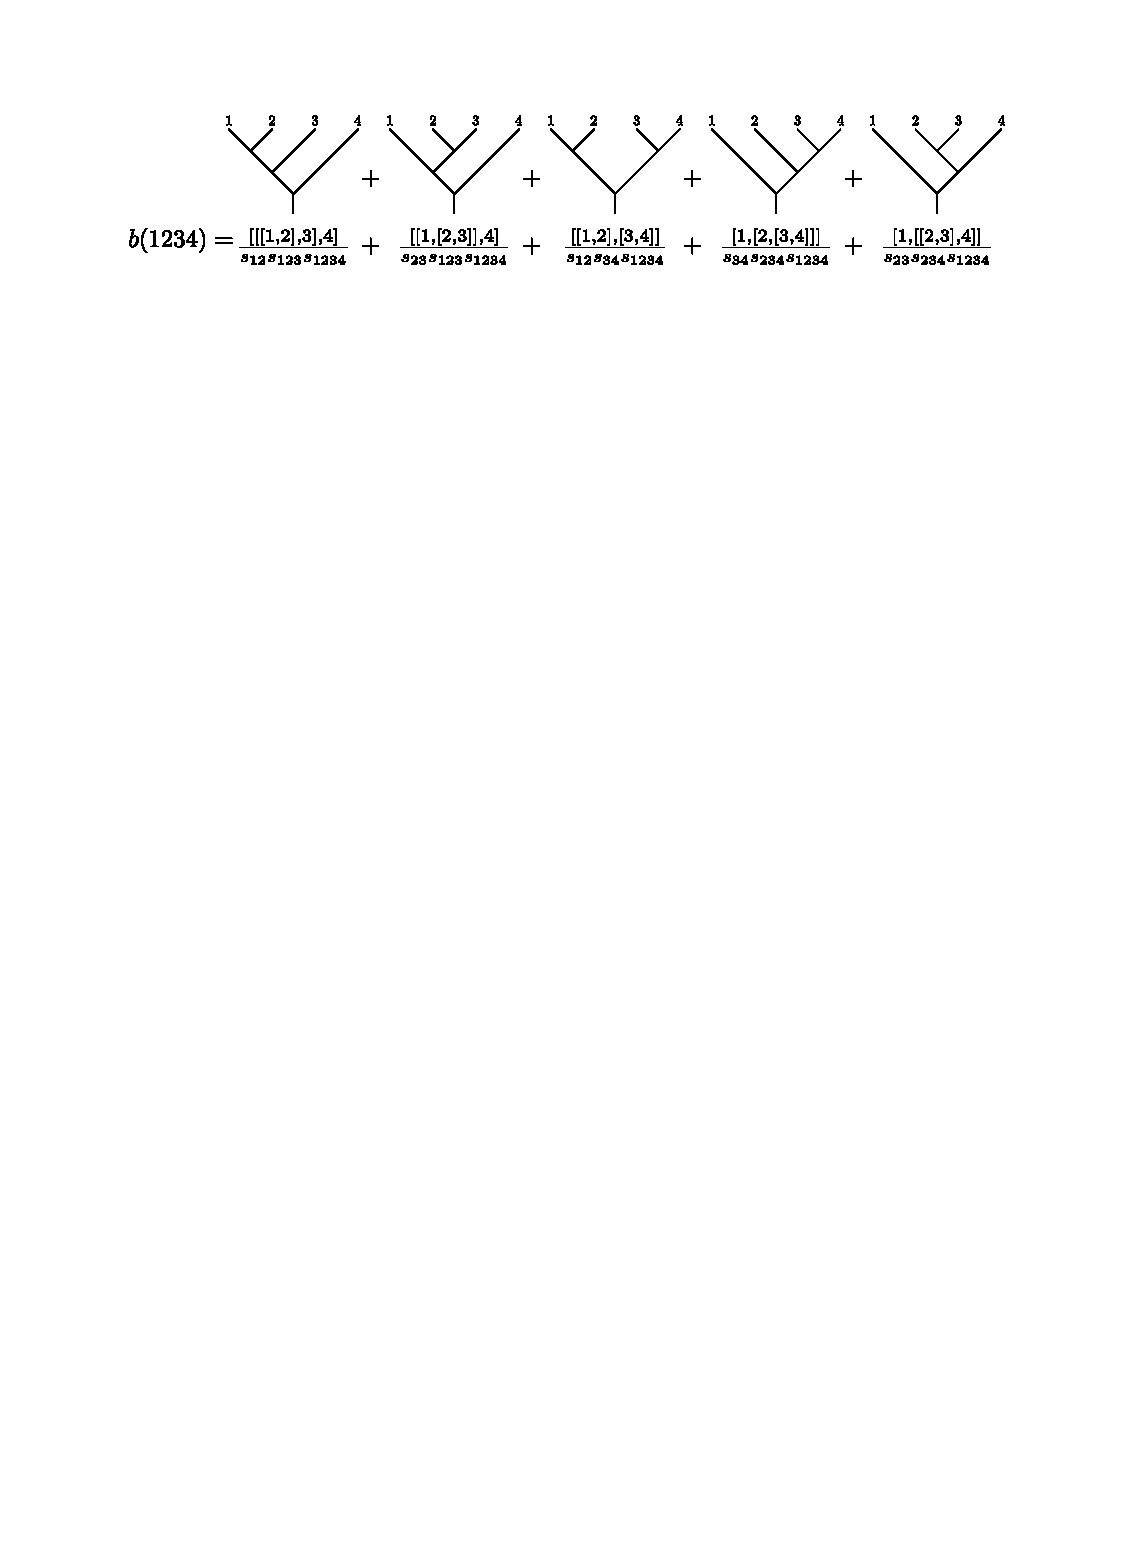
\includegraphics{figs/fig15.pdf}
	\caption{BG流的定义}
	\label{fig:6.6}
\end{figure}
\begin{figure}[htbp]
	\centering
	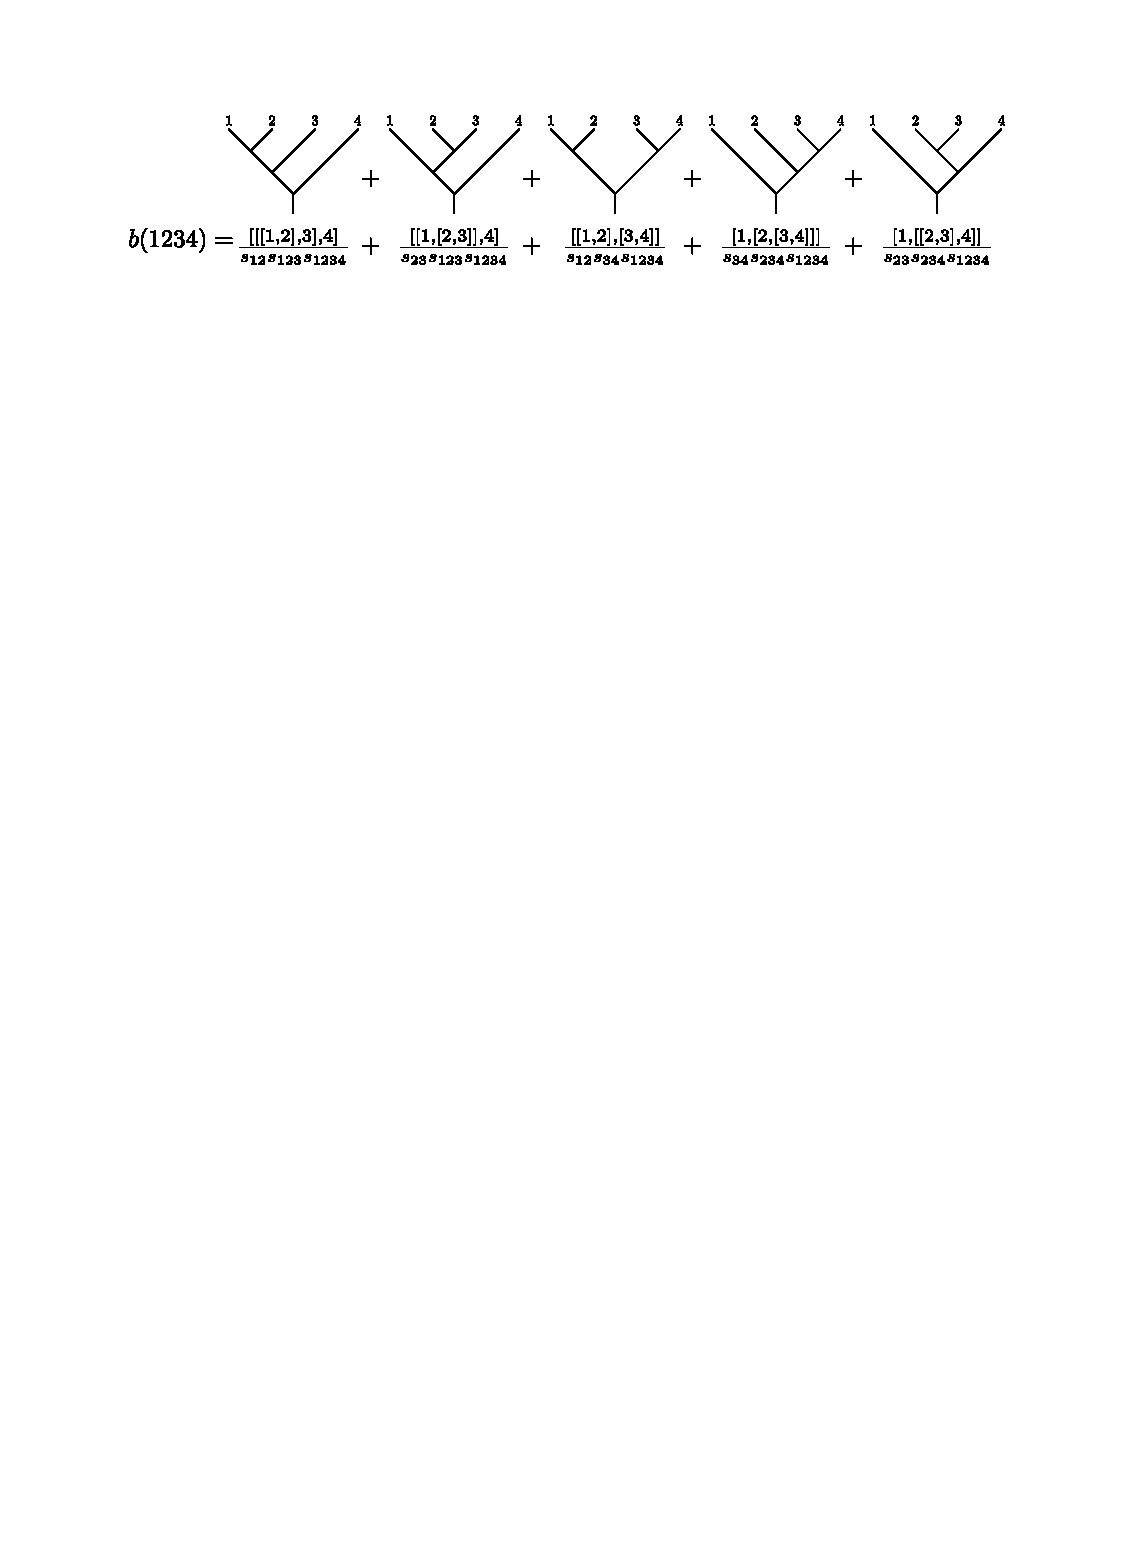
\includegraphics{figs/fig15.pdf}
	\caption{BG流的递推关系}
	\label{fig:6.7}
\end{figure}
从BG流的定义可以直接得到:
\begin{equation}
	\mathcal{A}_{n+1} =\lim_{k^2_{n+1}=0} \epsilon^\mu_{n+1}s_{1\cdots n}J_n
\end{equation}

所以只要通过离壳递推的方式计算出BG流,就能计算出振幅本身,类似的也可以定义色序振幅BG流。显然,这种递推是极其低效的,尽管如此这种方法还是率先用于计算得到了$n$点胶子MHV振幅的Park-Taylor公式\cite{Dixon:1996wi,Mangano:1990by}。场论树级振幅本质上是在求解经典运动方程,所以BG流应当也可以从经典运动方程求解得到,这发展成了Perturbiner方法,文献\cite{Mizera:2018jbh}中有不错的介绍。

比如对于Yang-Mills理论,考虑色序振幅BG流,Yang-Mills方程为:
\begin{equation}
	\square\mathbb{A}^{\mu}=[\mathbb{A}_{\nu},\partial^{\nu}\mathbb{A}^{\mu}+\mathbb{F}^{\nu\mu}]
\end{equation}
然后取拟设:
\begin{equation}
	\mathbb{A}^\mu(x):=\sum_PA_P^\mu T^Pe^{k_P\cdot x}=\sum_iA_i^\mu T^{a_i}e^{k_i\cdot x}+\sum_{i,j}A_{ij}^\mu T^{a_i}T^{a_j}e^{k_{ij}\cdot x}+\ldots
\end{equation}
从物理上看无非就是在壳粒子取平面波拟设,$T$是在壳粒子带的色因子,而前面的$A$便是一条外腿离壳得来的平面波。所以可以通过平面波拟设解方程的方式得到BG流。

用同样的方法解(非线性)超场方程\ref{eq:5.43}可以得到SYM的BG流:\cite{Lee:2015upy}
\begin{equation}
	\begin{aligned}
		&\mathcal{A}_{\alpha}^{[P,Q]}=\frac{1}{2}\left[\mathcal{A}_\alpha^  {Q}(k_Q\cdot\mathcal{A}_P)+\mathcal{A}_  {Q}^m(\gamma_m\mathcal{W}_P)_\alpha-(P\leftrightarrow  {Q})\right],\\&\mathcal{A}_{[P,  {Q}]}^m=\frac{1}{2}\left[\mathcal{A}_Q^m(k_Q\cdot\mathcal{A}_P)+\mathcal{A}_n^Q\mathcal{F}_P^{mn}+(\mathcal{W}_P\gamma^m\mathcal{W}_  {Q})-(P\leftrightarrow  Q)\right],\\&\mathcal{W}_{[P,  {Q}]}^{\alpha}=\frac{1}{2}\left[\mathcal{W}_Q^\alpha(k_Q\cdot\mathcal{A}_P)+\mathcal{W}_Q^{m\alpha}\mathcal{A}_P^m+\frac{1}{2}\mathcal{F}_P^{rs}(\gamma_{rs}\mathcal{W}_Q)^\alpha-(P\leftrightarrow  Q)\right],\\&\mathcal{F}_{[  {P},  {Q}]}^{mn}=\frac{1}{2}\left[\mathcal{F}_{  {Q}}^{mn}(k_{  {Q}}\cdot\mathcal{A}_{  {P}})+\mathcal{F}_{  {Q}}^{p|mn}\mathcal{A}_{p}^{p}+\mathcal{F}_{  {Q}}^{[m}{}_{r}\mathcal{F}_{P}^{n]r}+2(\mathcal{W}_{  {Q}}\gamma^{[m}\mathcal{W}_{P}^{n]})-(P\leftrightarrow  Q)\right]
	\end{aligned}
\end{equation}
递推起点为$\mathcal{K}_i = K_i$,同样BG流由于是离壳的,所以也涉及到规范的选取,如果递推起点改为$\mathcal{K}_i = \hat{K}_i$就是在Lorenz规范下的BG流。而且可以自然退化到YM理论的BG流$\mathcal{A}_{P}^{m}(\theta=0)|_{\chi_{i}=0}=J_{P}^{m}$。利用上面的递推式计算前三个BG流得到:\footnote{注意我们只是对BCJ超场取了$\ell(P):= P$的符号约定,这里BG流的下标只是单独的一个字词。}
\begin{equation}
	\begin{aligned}
		\mathcal{ K}_{12}^{m}&=\frac{ K_{[1,2]}^m}{s_{12}}\\
		\mathcal{ K}_{123}^{m}&=\frac{ K_{[[1,2],3]}^m}{s_{12}s_{123}}+\frac{ K_{[1,[2,3]]}^m}{s_{123}s_{23}}\\
		\mathcal{ K}_{1234}^m&=\frac{ K_{[[[1,2],3],4]}^m}{s_{12}s_{123}s_{1234}}+\frac{ K_{[[1,[2,3]],4]}^m}{s_{123}s_{1234}s_{23}}+\frac{ K_{[[1,2],[3,4]]}^m}{s_{12}s_{1234}s_{34}}+\frac{ K_{[1,[[2,3],4]]}^m}{s_{1234}s_{23}s_{234}}+\frac{ K_{[1,[2,[3,4]]]}^m}{s_{1234}s_{234}s_{34}}
	\end{aligned}
\end{equation}
递归定义平面二叉树求和\cite{Mafra:2020qst},示例见图\ref{fig:6.8}:\footnote{$s_P:=\frac12 k_P^2$,注意我们本章选取了$ik\to k$的符号约定,所以后面计算结果中$s_P\to -s_P$才得到保留虚数单位时的符号约定。}
%% 在后面也要写一下
\begin{equation}
	b(P):=\frac{1}{s_P}\sum_{XY=P}[b(X),b(Y)],\quad b(i):=i,\quad b(\varnothing):=0
\end{equation}
\begin{figure}[htbp]
	\centering
	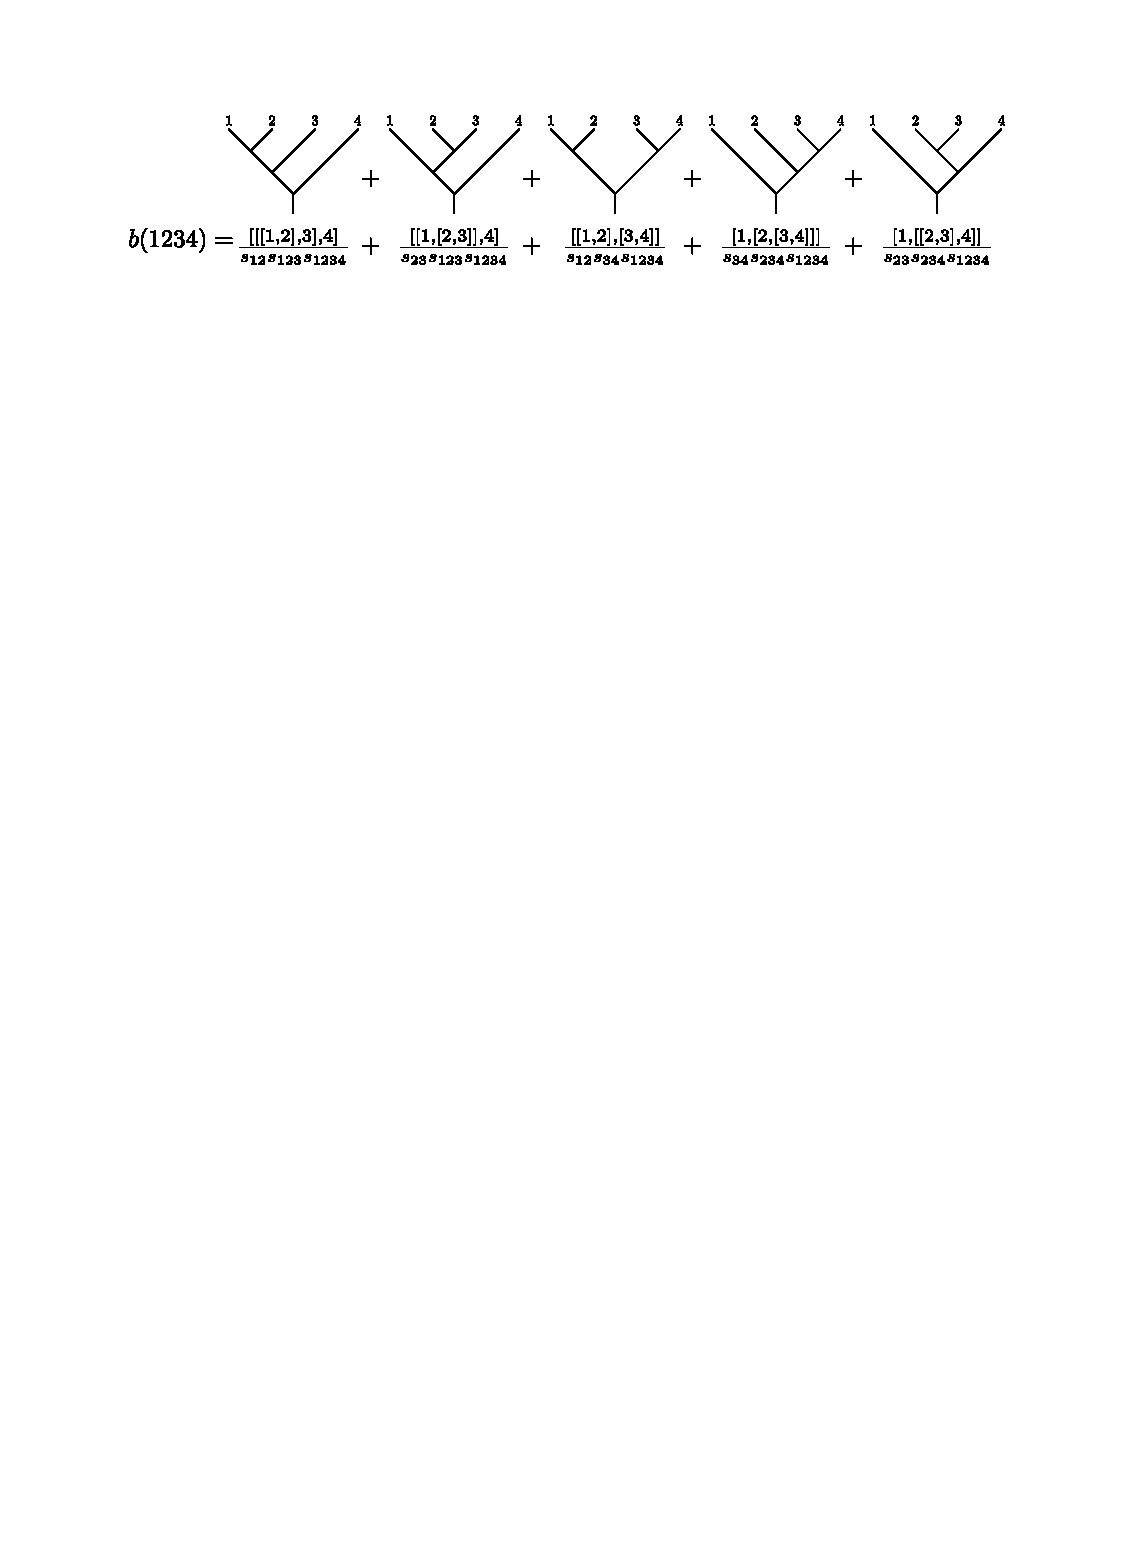
\includegraphics[width=\linewidth]{figs/fig15.pdf}
	\caption{平面二叉树求和}
	\label{fig:6.8}
\end{figure}
所以BG流和超场之间可以用下面的等式联系:
\begin{equation}
	\boxed{
		\mathcal{K}_P=K_{b(P)}
	}
\end{equation}
同理对Lorenz规范有$\mathcal{K}_P=K_{b(P)}$,这不仅能简化计算,后面会看到BG流的对称性可以从$b$算符本身的对称性很快得出。

但是后面构造SYM振幅并不用超场对应的这个BG流$\mathcal{K}$构造,而是利用纯旋量空间的类似物:
\begin{equation}
	M_P=\lambda^\alpha\mathcal{A}_\alpha^P
\end{equation}
这个是后面递推会用到的BG流。同理有$M_P=V_{b(P)}$。
\subsection{自由李代数对称性}
平面二叉树映射有个很重要的性质是自伴性:
\begin{equation}
	\label{eq:6.55}
	\langle b(P),Q\rangle=\langle P,b(Q)\rangle
\end{equation}
其证明只要注意到:
\begin{equation}
\begin{gathered}
		\langle b(P),Q\rangle=\frac{1}{s_P}\sum_{XY=P}\langle b(X)b(Y),Q\rangle-(X\leftrightarrow Y)\\
	\langle AB,RS\rangle=\langle A,R\rangle\langle B,S\rangle,\quad|A|=|R|,\quad|B|=|S|
\end{gathered}
\end{equation}
然后对$|P|$进行数学归纳便可得证,洗牌序有下面的重要定理:
\begin{boxedtext}[Ree定理]
	任取非空字词$\Gamma$,$R$和$S$,满足下式:
	\begin{equation}
		\langle\Gamma,R\shuffle S\rangle=0,\quad R,S\neq\varnothing
	\end{equation}
\end{boxedtext}
利用\ref{eq:6.55}以及Ree定理立刻得到:
\begin{equation}
\begin{aligned}
	\label{eq:6.58}
		&0=\langle b(P),R\shuffle S\rangle=\langle P,b(R\shuffle S)\rangle,\quad R,S\neq\emptyset,\quad\forall P\\
	\Rightarrow &b(A\shuffle B)=0,\quad\forall A,B\neq\emptyset
\end{aligned}
\end{equation}
这意味着BG流有下面的对称性:
\begin{equation}
	\mathcal{K}_{A\shuffle B}=0,\quad\forall A,B\neq\varnothing
\end{equation}
这是BG流非常重要的对称性,从这里看来只是自由李代数的简单应用,文献\cite{Frost:2020eoa}中有更多类似的讨论,其中$S$括号$\{\bullet,\bullet\}$的定义比较有用:
\begin{equation}
	\{P,Q\}=\sum_{\substack{XiY=P\\{ { {RjS=Q}}}}}k_i\cdot k_j(X \shuffle\tilde{Y})ij(\tilde{R} \shuffle S)(-1)^{|Y|+|R|}
\end{equation}
注意$S$括号定义在$\mathcal{L}^*\times \mathcal{L}^*\to\mathcal{L}^*$,$\mathcal{L}$是李多项式所在的线性空间$\mathcal{L}^*$是其对偶空间,在这里我们可以理解为商空间$\mathcal{L}/\sim$,其中:
\begin{equation}
	A\sim B\Leftrightarrow A=B+\sum R\shuffle  S,R,S\neq\varnothing
\end{equation}
$S$括号有下面的性质:
\begin{equation}
	\{A\shuffle B,C\}=0,\quad b(\{P,Q\})=[b(P),b(Q)],\quad \sum_{XY=P}\{X,Y\}\sim s_PP
\end{equation}
而且$S$括号实际上是$C$映射的伴随算子:
\begin{equation}
	\langle P\otimes Q,C(\Gamma)\rangle=\langle\{P,Q\},\Gamma\rangle
\end{equation}
$C$映射有下面重要的恒等式:
\begin{align}
	C(\ell(P))&=\sum_{\substack{XjY=P\\\delta(Y)=R\otimes S}}(k_X\cdot k_j)\left[\ell(XR)\otimes\ell(jS)-\ell(jR)\otimes\ell(XS)\right]\notag\\
	&=\sum_{\substack{XjY=P\\\delta(Y)=R\otimes S}}(k_X\cdot k_j)\ell(XR)\wedge\ell(jS)\\
	C(P\wedge Q)&=C(P)\wedge Q-P\wedge C(Q)\\
	\label{eq:6.66}
	C\left(b(P)\right)&=\sum_{XY=P}\left(b(X)\otimes b(Y)-b(Y)\otimes b(X)\right):=\sum_{XY=P}b(X)\wedge b(Y)
\end{align}
利用第上面第一个等式:
\begin{equation}
	C(\ell(123))=(k_1\cdot k_2)\left(\ell(1)\wedge\ell(23)+\ell(13)\wedge\ell(2)\right)+(k_{12}\cdot k_3)\ell(12)\wedge\ell(3)
\end{equation}
再利用\ref{eq:6.46},并且注意到$V_P:=V_{\ell(P)}$:
\begin{equation}
	QV_{123}=(k_1\cdot k_2)\left(V_1V_{23}+V_{13}V_2\right)+(k_{12}\cdot k_3)V_{12}V_3
\end{equation}
可以看到两式数学结构完全一致!$VV$之间的OPE乘法在自由李代数中被替换为了反对易的$\wedge$,而$V$恰好是费米算符!而且从组合学上可以证明$C^2=0$。结合前面所有的讨论,我们可以断言超场之于下标的作用正如$C$,$\ell$和$b$之于字词的作用:
\begin{equation}
	\label{eq:6.69}
	\boxed{
		C\leftrightarrow Q_{\mathrm{BRST}},\quad\ell(P)\leftrightarrow V_P/K_P,\quad b(P)\leftrightarrow M_P/\mathcal{K}_P
	}
\end{equation}
这就是BG流/多粒子超场和自由李代数之间的深刻关联。对于$\ell(P)$形式的多粒子顶角算符,\ref{eq:6.46}其实可以改写为:
\begin{equation}
	QV_\Gamma:=QV_\ell(\Gamma)=(V\wedge V)_{\mathbb{C}(\Gamma)}
\end{equation}
现在利用\ref{eq:6.66}得到:
\begin{equation}
	\label{eq:6.71}
\begin{aligned}
		QM_P&=QV_{b(P)}=(V\wedge V)_{C(b(P))}=\sum_{XY=P}(V\wedge V)_{b(X)\wedge b(Y)}=\sum_{XY=P}V_{b(X)}V_{b(Y)}\\
	&=\sum_{XY=P}M_XM_Y
\end{aligned}
\end{equation}
还有一个比较重要的KLT映射,我们用$\mathcal{S}:\mathcal{L}\to\mathcal{L}^*$表示,他的定义是将所有$\Gamma$中的李括号$[\bullet,\bullet]$改为$S$括号$\{\bullet,\bullet\}$,变换后的李多项式记作$\{\Gamma\}$。由此定义广义KLT核:
\begin{equation}
	\mathcal{S}^\ell(P| Q)=\langle\{\ell(P)\},\ell( Q)\rangle
\end{equation}
KLT关系中的固定$i,n-1,n$三条外腿的KLT核是上面的特殊形式:
\begin{equation}
	S(P|Q)_i=S^\ell(iP|iQ)
\end{equation}
其满足下面的递推式:\cite{Carrasco:2016ldy}
\begin{equation}
	S(Aj|BjC)_i=k_j\cdot k_{iB}S(A|BC)_i,\quad S(\varnothing|\varnothing)_i:=1
\end{equation}
KLT映射和$b$映射之间互逆,也就是说
\begin{equation}
	\label{eq:6.75}
	\mathcal{S}\circ b = \mathrm{id}_{\mathcal{L}^*},\quad b\circ \mathcal{S} = \mathrm{id}_{\mathcal{L}}
\end{equation}
一个词$P$称为是Lyndon的当且仅当在所有的$\mathrm{cyc}(P)$中$P$在字典序的意义下最小。Lyndon词可以作为$\mathcal{L}^*$的一组基底,$\ell(P)$则是$\mathcal{L}$的一组自然基底。所以$\{\ell(P)\}$可以在Lyndon基底下展开:\footnote{严格来说因为$\mathcal{L}^*$是在商空间的意义下定义的,下面的$=$应当替换为$\sim$。}
\begin{equation}
	\label{eq:6.76}
	\{\ell( {P})\}=\sum_{ {Q}\in \mathrm{Lyndon}}\langle\{\ell( {P})\},\ell( {Q})\rangle {Q}
\end{equation}
等式两边作用$b$映射并利用\ref{eq:6.75}得到:
\begin{equation}
	\ell(P)=b(\{\ell(  {P})\})=\sum_{  {Q}\in\mathrm{Lyndon}}\langle\{\ell(  {P})\},\ell(  {Q})\rangle b(  {Q})=\sum_QS^\ell(P|iQ)b(iQ)
\end{equation}
这里最后一个等号利用KLT核只有在$P$和$Q$中元素相同时不为零简化了求和计算,$i$是$P$中最小的字,$Q$表示$P/\{i\}$的字组成的词。把$P$也改写为$iP$ Lyndon词的形式,并利用\ref{eq:6.69}给出的对应得到:
\begin{equation}
	\label{eq:6.78}
	V_{iP}=\sum_{Q}S(P|Q)_iM_{iQ},\quad K_{iP}=\sum_{Q}S(P|Q)_i\mathcal{K}_{iQ}
\end{equation}
同样利用\ref{eq:6.76}类似的基底展开式可以证明下面的Schocker恒等式:
\begin{equation}
	B i A \sim (-1)^{|B|} i A \shuffle\tilde{B}
\end{equation}
再利用\ref{eq:6.69}的对应,只有$b$才能除去等价模掉的$R\shuffle S$的影响(\ref{eq:6.58}),给出:
\begin{equation}
	\label{schocker}
	\mathcal{K}_{B1A}=(-1)^{|B|}\mathcal{K}_{1(A\shuffle\tilde{B})}
\end{equation}
对$M$也同样成立。

回到一开始为了简化OPE的想法,我们研究了这么多多粒子超场的性质,都是为了顶角算符OPE变得有规律些:
\begin{equation}
	\label{eq:6.79}
	V_A(z_a)U_B(z_b)\to\frac{V_{[A,B]}(z_b)}{z_{ab}},\quad U_A(z_a)U_B(z_b)\to\frac{U_{[A,B]}(z_b)}{z_{ab}}
\end{equation}
这种简化后的OPE使得超弦$n$点盘面振幅计算变得可能。

\section{超弦无质量态$n$点盘面振幅}
取$z_n=\infty$的约定,现在利用\ref{eq:6.79}进行类似$\S$\ref{sec:5.4}的计算,只是顶角算符被看作了一个整体,比如四点OPE:
\begin{equation}
	\label{eq:6.80}
	\begin{aligned}
		V_1(z_1)U_2(z_2)V_3(z_3)V_4(\infty)&=\wick{\c V_1\c U_2V_3V_4}+\wick{ V_1\c U_2\c V_3V_4}+\wick{V_1\c U_2V_3\c V_4}\\
		&\cong\frac{V_{[1,2]}(z_1)}{z_{12}}V_3(z_3)V_4(\infty)+V_1(z_1)\frac{V_{[2,3]}(z_3)}{z_{23}}V_4(\infty)\\&\cong\frac{V_{12}V_3V_4}{z_{12}}+\frac{V_1V_{32}V_4}{z_{32}}
	\end{aligned}
\end{equation}
第二步利用了$z_4\to\infty$,所以任何与$V_4$的OPE均会被压低,第三步利用了$VV$之间OPE平凡。类似的对$n$点情况计算得到OPE:
\begin{equation}
	V_1\cdots U_i\cdots V_{n-1}V_n\cong\sum_{AB=23...n-2}(V_{1A}\mathcal{Z}_{1A})(V_{n-1,\tilde{B}}\mathcal{Z}_{n-1,\tilde{B}})V_n+\mathrm{perm}(2,3,...,n-2)
\end{equation}
其中Park-Taylor因子定义为:
\begin{equation}
	\mathcal{Z}_{123...p}:=\frac{1}{z_{12}z_{23}\ldots z_{p-1,p}}
\end{equation}
类似在RNS超弦振幅计算中所做的,对关联函数取不同盘面顺序积分得到相应的色序振幅,只不过我们这里还需要额外对零模积分:
\begin{equation}
	\label{eq:6.85}
\boxed{
		\mathcal{A}_n(P)=(2\alpha^{\prime})^{n-3}\int d\mu_P^n\sum_{AB=23...n-2}\langle\left(V_{1A}\mathcal{Z}_{1A}\right)(V_{n-1,\tilde{B}}\mathcal{Z}_{n-1,\tilde{B}})V_n\rangle+\mathrm{perm}(23\ldots n-2)
}
\end{equation}
这里积分测度为带Koba-Nielsen因子的$SL(2,\mathbb{C})$不变测度:\footnote{似乎和前面$\S$4计算出来的KN因子不同,这是因为我们选取了$ik\to k$的符号约定,所以$s\to -s$。}
\begin{equation}
	\int d\mu_P^n:=\int_{D(P)}dz_2dz_3\cdots dz_{n-2}\prod_{1\leq i<j}^{n-1}|z_{ij}|^{-2\alpha^{\prime}s_{ij}}
\end{equation}
同样$z_1$和$z_{n-1}$的坐标约定选取$\{0,1\}$或$\{1,0\}$应当与排序$P$相容。比如利用\ref{eq:6.80},四点振幅为:
\begin{equation}
	\begin{aligned}
		\mathcal{A}(1,2,3,4)&=2\alpha^{\prime}\int_0^1dz_2\left(\frac{\langle V_{12}V_3V_4\rangle}{z_{12}}+\frac{\langle V_1V_{32}V_4\rangle}{z_{32}}\right)|z_{12}|^{-2\alpha^{\prime}s_{12}}|z_{23}|^{-2\alpha^{\prime}s_{23}}\\&=\left(\frac{\langle V_{12}V_3V_4\rangle}{s_{12}}+\frac{\langle V_1V_{23}V_4\rangle}{s_{23}}\right)\frac{\Gamma(1-2\alpha^{\prime}s_{12})\Gamma(1-2\alpha^{\prime}s_{23})}{\Gamma(1-2\alpha^{\prime}s_{12}-2\alpha^{\prime}s_{23})}
	\end{aligned}
\end{equation}
定义一个同样对下标满足广义BCJ恒等式\ref{eq:6.38}的变量:
\begin{equation}
	X_{P}:=\frac{1}{|P|}\sum_{ {Q}}S^{\ell}(P| {Q})\mathcal{Z}_{ {Q}}=\prod_{j=2}^{|P|}\sum_{i=1}^{j-1}\frac{s_{p_ip_j}}{z_{p_ip_j}}
\end{equation}
其满足下面的积分恒等式:
\begin{equation}
	\label{eq:6.87}
	\int d\mu_P^nX_{1A}X_{(n-1)\tilde{B}}=(-1)^{|B|}\int d\mu_P^nX_{1AB}
\end{equation}
我们举五点的例子来说明,首先注意到由于KN因子包含每两个点坐标之差,所以有:
\begin{equation}
	\int_{z_a}^{z_b}dz_k\frac{\partial}{\partial z_k}\frac{\prod_{1\leq i<j}^{n-1}|z_{ij}|^{-2\alpha^{\prime}s_{ij}}}{z_{i_1j_1}\cdots z_{i_{n-4}j_{n-4}}}=0
\end{equation}
考虑$z_k$不在分母中出现的特殊情况,比如五点情况作用$\partial_{z_3}$得到:
\begin{equation}
	\int_{D(P)}dz_2dz_3\prod_{1\leq i<j}^4|z_{ij}|^{-2\alpha^{\prime}s_{ij}}
	\eqnmarkbox[blue]{node1}{\frac{s_{12}}{z_{12}}\left(\frac{s_{13}}{z_{13}}+\frac{s_{23}}{z_{23}}\right)}
	=\int_{D(P)}dz_2dz_3\prod_{1\leq i<j}^4|z_{ij}|^{-2\alpha^{\prime}s_{ij}}
	\eqnmarkbox[red]{node2}{\frac{s_{12}}{z_{12}}\frac{s_{34}}{z_{34}}}
\end{equation}
\annotate[yshift=0em]{below,left}{node1}{$X_{123}$}
\annotate[yshift=+0.5em]{above,left}{node2}{$X_{12}\cdot X_{34}$}
将\ref{eq:6.87}与\ref{schocker}结合得到:
\begin{equation}
	\int d\mu_P^n(M_{1A}X_{1A})(M_{n-1\tilde{B}}X_{(n-1)\tilde{B}})=\int d\mu_P^nX_{1AB}M_{1A}M_{B(n-1)}
\end{equation}
另外从\ref{eq:6.78}可以看到:
\begin{equation}
	\sum_AV_{iA}Z_{iA}=\sum_AM_{iA}X_{iA}
\end{equation}
利用这两个式子就能将\ref{eq:6.85}改用$M_P$表达,比如四点情况:
\begin{equation}
\begin{aligned}
		\mathcal{A}_4(P)&=2\alpha^{\prime}\int d\mu_P^4\left\langle V_{12}\mathcal{Z}_{12}V_3V_4+V_1V_{32}\mathcal{Z}_{32}V_4\right\rangle\\
	&=2\alpha^{\prime}\int d\mu_{P}^{4}\left\langle X_{12}M_{12}M_{3}M_{4}+X_{32}M_{1}M_{32}M_{4}\right\rangle\\
	&=2\alpha^{\prime}\int d\mu_P^4X_{12}\langle M_{12}M_3M_4+M_1M_{23}M_4\rangle
\end{aligned}
\end{equation}
对于任意点有:
\begin{equation}
\boxed{
		\mathcal{A}_n(P)=(2\alpha^{\prime})^{n-3}\int d\mu_P^n\left[\prod_{k=2}^{n-2}\sum_{m=1}^{k-1}\frac{s_{mk}}{z_{mk}}A_n(1,2,\ldots,n)+\mathrm{perm}(2,3,\ldots,n-2)\right]
}
\end{equation}
其中:
\begin{equation}
	\label{eq:6.96}
\boxed{
		A_n(P,n):=\sum_{XY=P}\langle M_XM_YM_n\rangle
}
\end{equation}
考虑固定三个外腿顺序的情况:
\begin{equation}
	\mathcal{A}_n(1,R,n-1,n;\alpha^{\prime})=\sum_{{Q}\in S_{n-3}}{{F}_R}^{Q}(\alpha^{\prime})A_n(1,{Q},n-1,n)
\end{equation}
其中:
\begin{equation}
\begin{aligned}
	\label{eq:6.98}
		{F_R}^Q(\alpha^{\prime}):=&(2\alpha^{\prime})^{n-3}\int d\mu_R^n\frac{s_{1q_2}}{z_{1q_2}}\left(\frac{s_{1q_3}}{z_{1q_3}}+\frac{s_{q_2q_3}}{z_{q_2q_3}}\right)
	\times\left(\frac{s_{1q_4}}{z_{1q_4}}+\frac{s_{q_2q_4}}{z_{q_2q_4}}+\frac{s_{q_3q_4}}{z_{q_3q_4}}\right)\cdots\\
	&\times\left(\frac{s_{1q_{n-2}}}{z_{1q_{n-2}}}+\frac{s_{q_2q_{n-2}}}{z_{q_2q_{n-2}}}+\cdots+\frac{s_{q_{n-3}q_{n-2}}}{z_{q_{n-3}q_{n-2}}}\right)
\end{aligned}
\end{equation}
\section{SYM振幅的纯旋量超空间上同调表述}
利用下面$\alpha'\to 0$的展开式:
\begin{equation}
	\log\Gamma(1-z)=\gamma z+\sum_{n=2}^\infty\frac{z^n}{n}\zeta_n
\end{equation}
$\gamma$是Euler常数,$\zeta$是黎曼$\zeta$函数,对四点情况展开\ref{eq:6.98}:
\begin{equation}
\begin{aligned}
		{F_2}^2&=\frac{\Gamma(1-2\alpha^{\prime}s_{12})\Gamma(1-2\alpha^{\prime}s_{23})}{\Gamma(1-2\alpha^{\prime}s_{12}-2\alpha^{\prime}s_{23})}=\exp\left(\sum_{n=2}^\infty\frac{\zeta_n}{n}(2\alpha^{\prime})^n\left[s_{12}^n+s_{23}^n-(s_{12}+s_{23})^n\right]\right)\\
	&=1-(2\alpha^{\prime})^2\zeta_2s_{12}s_{23}+\cdots
\end{aligned}
\end{equation}
其实,对于一般情况有:
\begin{equation}
	{F_P}^{Q}(\alpha^{\prime})=\delta_P^{Q}+\mathcal{O}({\alpha'}^2)
\end{equation}
这就说明\ref{eq:6.96}就是弦振幅的低能展开,也就是固定一个外腿$n$的SYM色序振幅!前面我们将$M_P$解释为纯旋量空间BG流的类似物,所以这里对SYM振幅的构造完全可以解释为用BG流拼凑得来,如图\ref{fig:6.9}。
\begin{figure}[htbp]
	\centering
	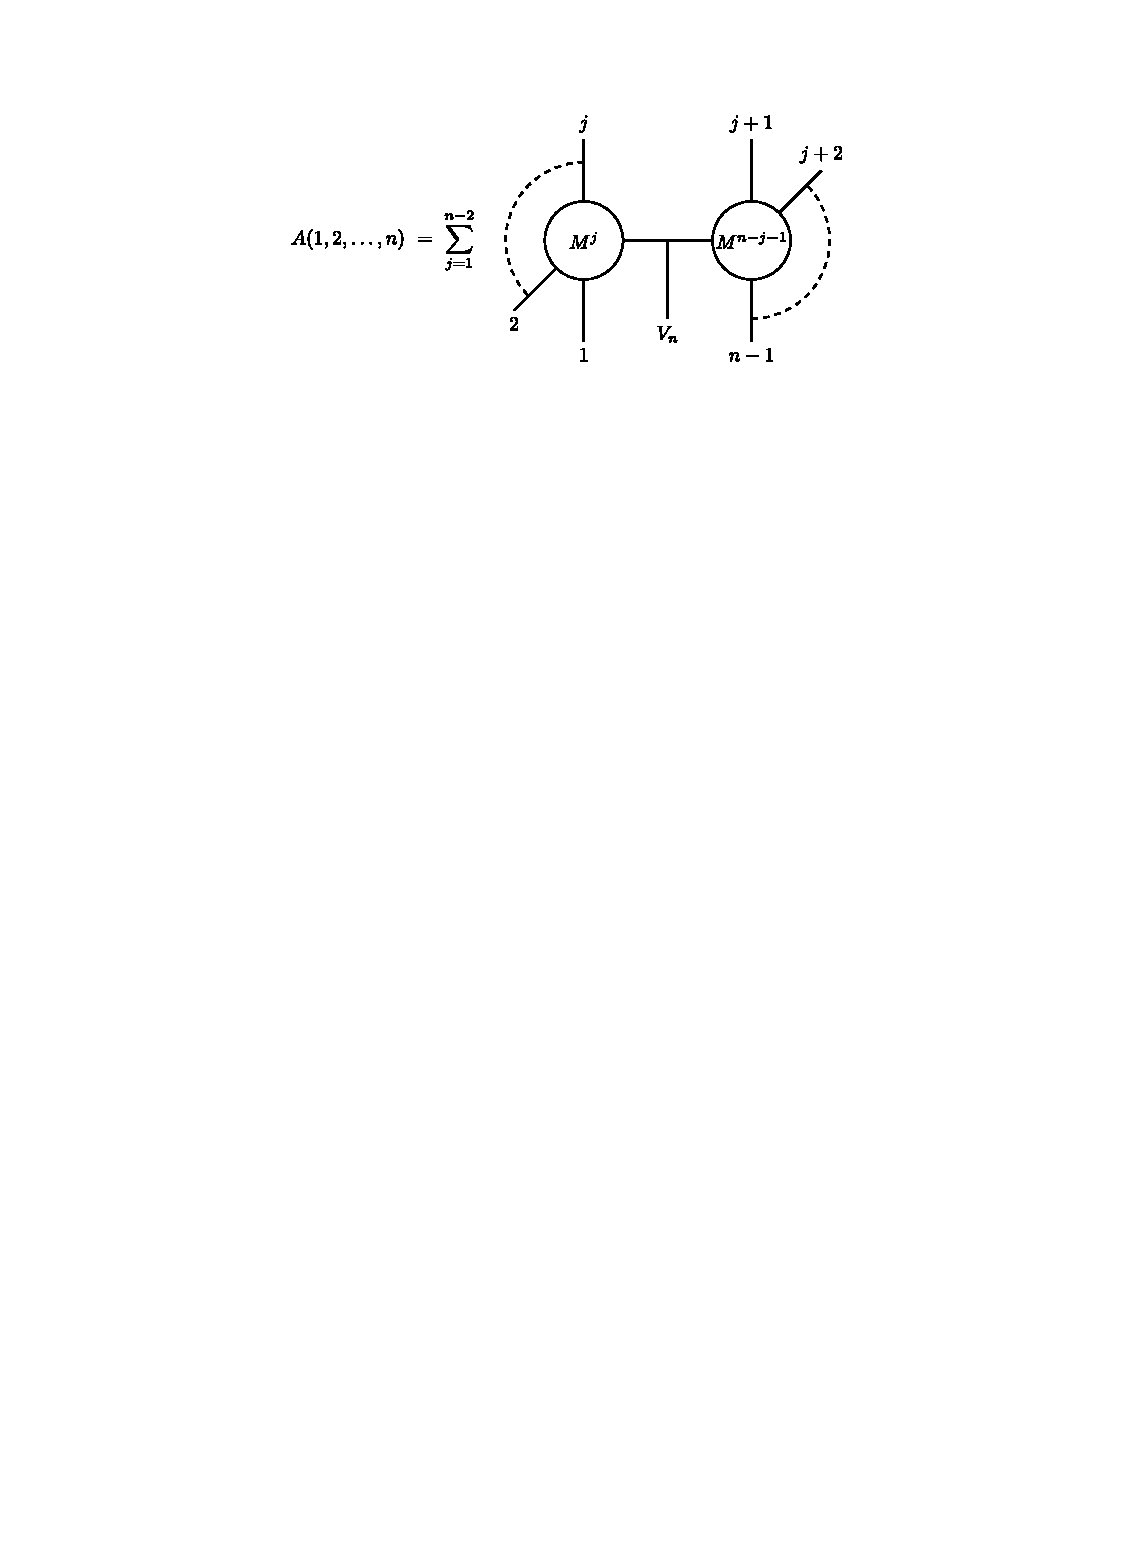
\includegraphics[width=0.8\linewidth]{figs/fig16.pdf}
	\caption{SYM振幅的纯旋量超空间上同调形式}
	\label{fig:6.9}
\end{figure}
注意到$QM_n=QV_n=0$,以及:
\begin{equation}
	\begin{aligned}
		\sum_{XY=P}Q(M_XM_Y)&=\sum_{XY=P}\sum_{RS=X}M_RM_SM_Y-\sum_{XY=P}\sum_{RS=Y}M_XM_RM_S\\&=\sum_{RSY=P}\left(M_RM_SM_Y-M_RM_SM_Y\right)=0
	\end{aligned}
\end{equation}
所以\ref{eq:6.96}是闭的,虽然看似根据\ref{eq:6.71}$\sum_{XY=P}M_XM_Y$是恰当的,但是由于$M_P$本身的定义包含$s_P$因子,所以对于这里$s_P=k_n^2=0$,也就是在壳时\ref{eq:6.71}不是良定义的,所以在壳时无法将$\sum_{XY=P}M_XM_Y$看作是恰当的,但离壳时可以。所以用\ref{eq:6.96}形式写下的算符明显地存在于纯旋量超空间的上同调群中。但是这种表述并没有明显地满足循环对称的要求,现在我们来证明循环变换指标只会导致一个BRST恰当项的差别,在关联函数的意义下为$0$。



任意点振幅都可以通过加上一些BRST恰当的项写成循环对称的形式,比如:
\begin{equation}
	A_7(1,2,\ldots,7)=\langle M_{123}M_{45}M_{67}\rangle+\langle M_1M_{234}M_{567}\rangle+\mathrm{cyc}(12\ldots7)
\end{equation}

原则上,$M_P$可以用$\mathcal{K}_P$表达,而$\mathcal{K}_P$又可以用$K_P$表达,而多粒子超场又可以用单粒子超场表达,单粒子超场$\theta$展开是已知的,所以原则上总可以通过这种方式计算出任意点SYM振幅。上述过程其实可以进一步简化,$\mathcal{K}$的$\theta$展开是可以直接计算的,由于最终只涉及到$M_P$,所以只需要$\mathcal{A}^P_\alpha$的展开:
\begin{equation}
	\mathcal{A}_\alpha^P(\theta)=\frac{1}{2}(\theta\gamma_m)_\alpha\mathfrak{e}_P^m+\frac{1}{3}(\theta\gamma^m)_\alpha(\theta\gamma_m\mathfrak{X}_P)-\frac{1}{32}(\theta\gamma^p)_\alpha(\theta\gamma_{mnp}\theta)\mathfrak{f}_P^{mn}+\cdots
\end{equation}
其中哥特体标注的多粒子极化矢量(波函数)有递推公式:\footnote{形式上很像是“BG流的BG流”。}
\begin{align*}
	&\mathfrak{e}_P^m=\frac{1}{s_P}\sum_{XY=P}\mathfrak{e}_{[X,Y]}^m,\quad\mathfrak{X}_P^\alpha=\frac{1}{s_P}\sum_{XY=P}\mathfrak{X}_{[X,Y]}^\alpha\\
	&\mathfrak{f}_P^{mn}:=k_P^m\mathfrak{e}_P^n-k_P^n\mathfrak{e}_P^m-\sum_{XY=P}\left(\mathfrak{e}_X^m\mathfrak{e}_Y^n-\mathfrak{e}_X^n\mathfrak{e}_Y^m\right)\\
	&\mathfrak{e}_{[X,Y]}^m:=\frac{1}{2}\left[\mathfrak{e}_Y^m(k_Y\cdot\mathfrak{e}_X)+\mathfrak{e}_n^X\mathfrak{f}_Y^{nm}+( X_X\gamma^m X_Y)-(X\leftrightarrow Y)\right]\\
	& \mathfrak{X}_{[X,Y]}^\alpha:=\frac{1}{2}(k_X^p+k_Y^p)\gamma_p^{\alpha\beta}\left[\mathfrak{e}_X^m(\gamma_m \mathfrak{X}_Y)_\beta-\mathfrak{e}_Y^m(\gamma_m \mathfrak{X}_X)_\beta\right]
\end{align*}
递推起点为$\mathfrak{e}_i^m:=e_i^m$,$\mathfrak{X}_i^\alpha:=\chi_i^\alpha$。再利用附录\ref{appendix:B}给出的零模积分公式可以得到:
\begin{equation}
	\langle M_XM_YM_Z\rangle=\frac{1}{2}\mathfrak{e}_X^m\mathfrak{f}_Y^{mn}\mathfrak{e}_Z^n+(\mathfrak{X}_X\gamma_m\mathfrak{X}_Y)e_Z^m+\mathrm{cyc}(XYZ)
\end{equation}
从数值运算的角度从BG流出发的这个公式要快不少。\cite{Badger:2012uz}

由于我们将振幅表述为了多粒子顶角算符,而这又根据\ref{eq:6.69}可以和自由李代数的结构联系起来,所以振幅所满足的性质应当完全可以从组合学的意义上看出。

首先是KK关系,\ref{schocker}

其次是BCJ关系
\section{利用纯旋量超弦构造Super-Yang-Mills理论的树图BCJ分子}
	
	% 参考文献
	\printbibliography
	
	% 致谢
	\begin{acknowledgements}
	大学四年只不过是我人生大尺度结构的量子涨落。感谢女朋友产生算符的不存在性让我能专心完成这篇毕业论文。
\end{acknowledgements}

	
	% 附录
	\appendix
	% 附录

\chapter{本论文主要使用到的算符乘积展开}
\label{appendix:A}
本附录给出一些振幅计算中经常用到的OPE以及能动张量等CFT相关约定,以供查阅。
\section{自由CFT}
本节对应玻色弦世界面CFT。
\subsection{自由玻色CFT}
$XX$包含四项

另外,根据加倍技巧,对于BCFT,左右模之间的OPE不是$0$:
\begin{equation}
	X^\mu(z_1)\tilde X^\nu(\bar z_2)\sim X^\mu(z_1)X^\nu(z'_2)\sim -\frac{\alpha^{\prime}}{2}\ln|z_1-\overline{z}_2|
\end{equation}
不过弦论中开弦BCFT计算只涉及到实轴上插入,所以不必过于在意上式。而在实轴上源点及其镜像重合,所以左右模OPE和纯左模OPE都会贡献:
\begin{equation}
	 X^\mu (y_1) X^\nu(y_2) \sim -2\alpha'\ln |y_1-y_2|
\end{equation}
这从\ref{eq:4.36}也能直接看出来,这也印证了$\alpha'_{\text{cl}}\sim4\alpha'_{\text{op}}$。
\subsection{$bc$鬼场}
\section{$\mathcal{N}=1$ SCFT}
本节对应RNS超弦世界面CFT,玻色场OPE与上一节相同。
\subsection{自由费米CFT}

\subsection{$\beta\gamma$鬼场}

\section{纯旋量形式}
这里只讨论左模,作用量见\ref{eq:5.23},能动张量以及对应的超流(费米Lorentz流):
\begin{equation}
	T_{\mathrm{PS}} = :-\frac{1}{2} \Pi^\mu \Pi_\mu - d_\alpha \partial \theta^\alpha + w_\alpha \partial \lambda^\alpha:, \quad M^{\mu\nu} = \Sigma^{\mu\nu} + N^{\mu\nu} = :-\frac{1}{2} (p \gamma^{\mu\nu} \theta) + \frac{1}{2} (w \gamma^{\mu\nu} \lambda):
\end{equation}
其中$h(\lambda^\alpha) = 0$,$h(w_\alpha) = +1$。由于纯旋量约束,这并不是一个自由CFT:
\begin{equation}
	\begin{aligned}
		X^\mu(z,\overline{z}) X^\nu(w,\overline{w}) 
		&\sim -\eta^{\mu\nu} \ln|z-w|^2, 
		& d_\alpha(z) \theta^\beta(w) 
		&\sim \frac{\delta_\alpha^\beta}{z-w}, \\
		d_\alpha(z) d_\beta(w) 
		&\sim -\frac{\gamma_{\alpha\beta}^\mu \Pi_\mu(w)}{z-w}, 
		& d_\alpha(z) \Pi^\mu(w) 
		&\sim \frac{(\gamma^\mu \partial\theta(w))_\alpha}{z-w}, \\
		\Pi^\mu(z) \Pi^\nu(w) 
		&\sim -\frac{\eta^{\mu\nu}}{(z-w)^2},&
		\partial\theta^\alpha(z) \{ \partial\theta^\beta(w),\Pi^\mu(w),&N^{\mu\nu}(w) \} \sim \mathrm{regular}
	\end{aligned}
\end{equation}
对于任意的不显含$X,\theta$导数项的超场$K(X,\theta)$:\footnote{平面波就是一个最简单的例子。}
\begin{equation}
	\begin{aligned}
		d_\alpha(z) K\left(X(w,\overline{w}), \theta(w)\right) 
		&\sim \frac{D_\alpha K\left(X(w,\overline{w}), \theta(w)\right)}{z-w}, \\
		\Pi^\mu(z) K\left(X(w,\overline{w}), \theta(w)\right) 
		&\sim -\frac{\partial^\mu K\left(X(w,\overline{w}), \theta(w)\right)}{z-w}.
	\end{aligned}
\end{equation}
其中超空间导数为:
\begin{equation}
	D_\alpha=\frac{\partial}{\partial\theta^\alpha}+\frac{1}{2}(\gamma^\mu\theta)_\alpha\partial_\mu
\end{equation}
还有一些有关超流的OPE:
\begin{equation}
	\begin{aligned}
		M^{\mu\nu}(z) M^{\rho\sigma}(w) 
		&\sim \frac{\eta^{\rho[\mu} M^{\nu]\sigma}(w) - \eta^{\sigma[\mu} M^{\nu]\rho}(w)}{z-w} + \frac{\eta^{\mu[\sigma} \eta^{\rho]\nu}}{(z-w)^2}, \\
		N^{\mu\nu}(z) N^{\rho\sigma}(w) 
		&\sim \frac{\eta^{\rho[\mu} N^{\nu]\sigma}(w) - \eta^{\sigma[\mu} N^{\nu]\rho}(w)}{z-w} - 3 \frac{\eta^{\mu[\sigma} \eta^{\rho]\nu}}{(z-w)^2}, \\
		N^{\mu\nu}(z) \lambda^\alpha(w) 
		&\sim \frac{1}{2} \frac{(\gamma^{\mu\nu})^\alpha{}_\beta \lambda^\beta(w)}{z-w}.
	\end{aligned}
\end{equation}
	\chapter{一些常用的$\gamma$矩阵计算恒等式}
本附录默认$D=10$,且所有指标置换操作定义本身不带有$k!$因子。首先是一些符号约定:
\begin{equation}
\begin{aligned}
		\gamma^{\mu_1\mu_2...\mu_n} = \frac{1}{n!} \gamma^{[\mu_1} \gamma^{\mu_2} \cdots \gamma^{\mu_n]}\\
	\delta_{b_1b_2...b_n}^{a_1a_2...a_n}=\frac{1}{n!}\delta_{b_1}^{[a_1}\delta_{b_2}^{a_2}\cdots\delta_{b_n}^{a_n]}\\
	\epsilon_{01...9}=1,\quad\epsilon^{01...9}=-1
\end{aligned}
\end{equation}
Fierz恒等式为:
\begin{align}
		\psi^\alpha \chi^\beta &= \frac{1}{16} \gamma_{\mu_1}^{\alpha\beta} (\psi \gamma^{\mu_1} \chi) + \frac{1}{96} (\gamma_{\mu_1...\mu_3})^{\alpha\beta} (\psi \gamma^{\mu_1...\mu_3} \chi) + \frac{1}{3840} (\gamma_{\mu_1...\mu_5})^{\alpha\beta} (\psi \gamma^{\mu_1...\mu_5} \chi) \\
		\psi_\alpha \chi^\beta &= \frac{1}{16} \delta_\alpha^\beta (\psi \chi) + \frac{1}{32} (\gamma_{\mu_1\mu_2})_\alpha^\beta (\psi \gamma^{\mu_1\mu_2} \chi) + \frac{1}{384} (\gamma_{\mu_1...\mu_4})_\alpha^\beta (\psi \gamma^{\mu_1...\mu_4} \chi)
\end{align}
利用$\theta$的反对易性和$\lambda$的纯旋量性,上式有特殊情况:
\begin{equation}
	\lambda^\alpha \lambda^\beta = \frac{1}{3840} (\lambda \gamma^{\mu\nu\rho\sigma\tau} \lambda) \gamma_{\mu\nu\rho\sigma\tau}^{\alpha\beta}, \quad \theta^\alpha \theta^\beta = \frac{1}{96} (\theta \gamma^{\mu\nu\rho} \theta) \gamma_{\mu\nu\rho}^{\alpha\beta}
\end{equation}
$\gamma$矩阵的迹:
\begin{equation}
	\mathrm{Tr}\left(\gamma^P\gamma_Q\right)=16\delta^{p,q}\left[p!\delta_{Q^T}^P+\delta^{p,5}\epsilon_Q^P\right],\quad|P|:=p,\quad|Q|:=q
\end{equation}
对偶性:
\begin{equation}
	\begin{aligned}
		(\gamma^{\mu_1...\mu_5})_{\alpha\beta} 
		&= \frac{1}{5!} \epsilon^{\mu_1...\mu_5\nu_1...\nu_5} (\gamma_{\nu_1...\nu_5})_{\alpha\beta}, 
		& (\gamma^{\mu_1...\mu_5})^{\alpha\beta} 
		&= -\frac{1}{5!} \epsilon^{\mu_1...\mu_5\nu_1...\nu_5} (\gamma_{\nu_1...\nu_5})^{\alpha\beta}, \\
		(\gamma^{\mu_1...\mu_6})_{\alpha}^{\beta} 
		&= \frac{1}{4!} \epsilon^{\mu_1...\mu_6\nu_1...\nu_4} (\gamma_{\nu_1...\nu_4})_{\alpha}^{\beta}, 
		& (\gamma^{\mu_1...\mu_6})^{\alpha}_{\beta} 
		&= -\frac{1}{4!} \epsilon^{\mu_1...\mu_6\nu_1...\nu_4} (\gamma_{\nu_1...\nu_4})^{\alpha}_{\beta}, \\
		(\gamma^{\mu_1...\mu_7})_{\alpha\beta} 
		&= -\frac{1}{3!} \epsilon^{\mu_1...\mu_7\nu_1...\nu_3} (\gamma_{\nu_1...\nu_3})_{\alpha\beta}, 
		& (\gamma^{\mu_1...\mu_7})^{\alpha\beta} 
		&= \frac{1}{3!} \epsilon^{\mu_1...\mu_7\nu_1...\nu_3} (\gamma_{\nu_1...\nu_3})^{\alpha\beta}, \\
		(\gamma^{\mu_1...\mu_8})_{\alpha}^{\beta} 
		&= -\frac{1}{2!} \epsilon^{\mu_1...\mu_8\nu_1\nu_2} (\gamma_{\nu_1\nu_2})_{\alpha}^{\beta}, 
		& (\gamma^{\mu_1...\mu_8})^{\alpha}_{\beta} 
		&= \frac{1}{2!} \epsilon^{\mu_1...\mu_8\nu_1\nu_2} (\gamma_{\nu_1\nu_2})^{\alpha}_{\beta}, \\
		(\gamma^{\mu_1...\mu_9})_{\alpha\beta} 
		&= \epsilon^{\mu_1...\mu_9\nu_1} (\gamma_{\nu_1})_{\alpha\beta}, 
		& (\gamma^{\mu_1...\mu_9})^{\alpha\beta} 
		&= -\epsilon^{\mu_1...\mu_9\nu_1} (\gamma_{\nu_1})^{\alpha\beta}, \\
		(\gamma^{\mu_1...\mu_{10}})_{\alpha}^{\beta} 
		&= \epsilon^{\mu_1...\mu_{10}} \delta_{\alpha}^{\beta}, 
		& (\gamma^{\mu_1...\mu_{10}})^{\alpha}_{\beta} 
		&= -\epsilon^{\mu_1...\mu_{10}} \delta_{\beta}^{\alpha}.
	\end{aligned}
\end{equation}
$\gamma$矩阵的乘积:
\begin{equation}
	\gamma_{\mu_1\mu_2\ldots\mu_p} \gamma^{\nu_1\nu_2\ldots\nu_q} = \sum_{k=0}^{\min(p,q)} k! \binom{p}{k} \binom{q}{k} \delta_{[\mu_p}^{[\nu_1} \delta_{\mu_{p-1}}^{\nu_2} \cdots \delta_{\mu_{p-k+1}}^{\nu_k} {\gamma_{\mu_1\ldots\mu_{p-k}]}}^{\nu_{k+1}\ldots\nu_q]}
\end{equation}
其它常用等式:
\begin{align}
		\gamma_{\alpha(\beta}^\mu \gamma_{\gamma\delta)}^\mu &= 0, \\
		\gamma_{\alpha[\beta}^{\mu\nu\rho} \gamma_{\gamma\delta]}^{\mu\nu\rho} &= 0, \\
		\gamma_{\mu\nu\rho}^{\alpha\beta} \gamma_{\gamma\delta}^{\mu\nu\rho} &= 48 \left( \delta_\gamma^\alpha \delta_\delta^\beta - \delta_\gamma^\beta \delta_\delta^\alpha \right), \\
		\gamma_{\alpha\beta}^{\mu\nu\rho} \gamma_{\gamma\delta}^{\mu\nu\rho} &= 12 \left( \gamma_{\alpha\delta}^\mu \gamma_{\beta\gamma}^\mu - \gamma_{\alpha\gamma}^\mu \gamma_{\beta\delta}^\mu \right), \\
		\gamma_{\alpha\beta}^\mu \gamma_{\delta\sigma}^\mu &= -\frac{1}{2} \gamma_{\alpha\delta}^\mu \gamma_{\beta\sigma}^\mu - \frac{1}{24} \gamma_{\alpha\delta}^{\mu\nu\rho} \gamma_{\beta\sigma}^{\mu\nu\rho}, \\
		\gamma_{\alpha\beta}^{\mu\nu\rho} \gamma_{\delta\sigma}^{\mu\nu\rho} &= -18 \gamma_{\alpha\delta}^\mu \gamma_{\beta\sigma}^\mu + \frac{1}{2} \gamma_{\alpha\delta}^{\mu\nu\rho} \gamma_{\beta\sigma}^{\mu\nu\rho}, \\
		\gamma_{\alpha\beta}^{\mu\nu\rho} \gamma_{\delta\sigma}^{\mu\nu\rho} &= -12 \gamma_{\alpha\beta}^\mu \gamma_{\delta\sigma}^\mu - 24 \gamma_{\alpha\delta}^\mu \gamma_{\beta\sigma}^\mu, \\
		(\gamma^{\mu\nu})_\alpha^\delta (\gamma_{\mu\nu})_\beta^\sigma &= -8 \delta_\alpha^\sigma \delta_\beta^\delta - 2 \delta_\alpha^\delta \delta_\beta^\sigma + 4 \gamma_{\alpha\beta}^\mu \gamma_\mu^{\delta\sigma}, \\
		(\gamma^{\mu\nu\rho\sigma})_\alpha^\beta (\gamma_{\mu\nu\rho\sigma})_\sigma^\delta &= 315 \delta_{\alpha}^{\delta} \delta_{\sigma}^{\beta} + \frac{21}{2} (\gamma^{\mu\nu})_{\alpha}{}^{\delta} (\gamma_{\mu\nu})_{\sigma}{}^{\beta} + \frac{1}{8} (\gamma^{\mu\nu\rho\sigma})_{\alpha}{}^{\delta} (\gamma_{\mu\nu\rho\sigma})_{\sigma}{}^{\beta}, \\
		(\gamma^{\mu\nu\rho\sigma})_{\alpha}^{\beta} (\gamma_{\mu\nu\rho\sigma})_{\sigma}^{\delta} &= -48 \delta_\alpha^\beta \delta_\sigma^\delta + 288 \delta_\alpha^\delta \delta_\sigma^\beta + 48 \gamma_{\alpha\sigma}^\mu \gamma_\mu^{\beta\delta},\\
		\gamma_{\alpha\beta}^{\mu\nu\rho\sigma\tau} \gamma_{\delta\sigma}^{\mu\nu\rho\sigma\tau} &= 0, \\
		(\lambda \gamma^\mu)_\alpha (\lambda \gamma_\mu)_\beta &= 0, \\
		(\lambda \gamma_\mu)_\alpha (\lambda \gamma^{\mu\nu\rho\sigma\tau} \lambda) &= 0.
\end{align}
\end{document}